\documentclass[11pt, a4paper]{article}
\usepackage[margin=1in]{geometry}
\usepackage{graphicx}
\usepackage{amsmath, amssymb}
\usepackage{float}
\usepackage[utf8]{inputenc}
\title{Exhaustive Thesis Figure Generation Guide}
\author{Automatically Generated Reference}
\begin{document}
\maketitle
\tableofcontents
\clearpage

\section{Analytical Key Management}
\textbf{File:} \texttt{analytical\_key\_management.png} \\
\textbf{Concept/Origin:} This plot visualizes \textbf{Analytical Key Management Metric} as a function of \textbf{Time / Baseline Parameter}. \\
\textbf{Equations/Framework:} 
Empirical baseline calculation from simulation data.
\vspace{0.5cm}
\begin{figure}[H]
    \centering
    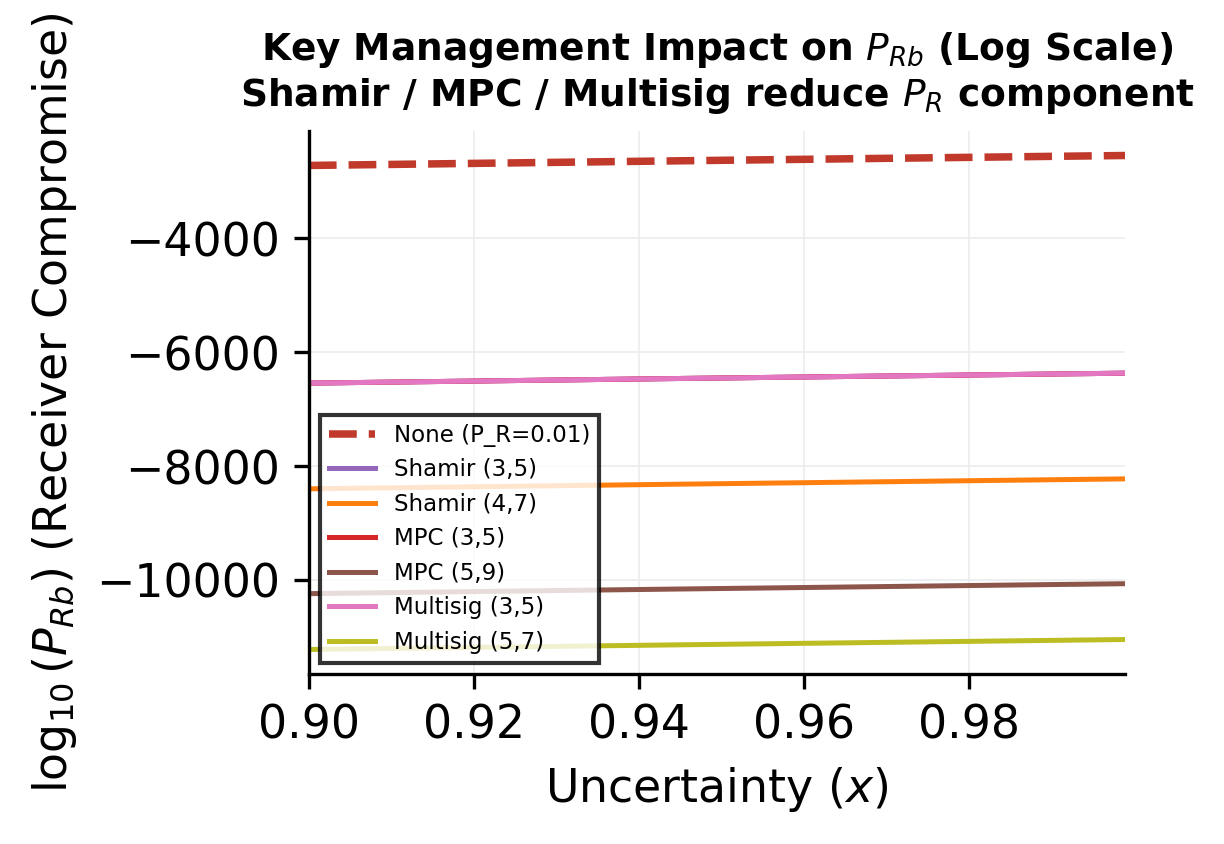
\includegraphics[width=0.75\textwidth]{figures/analytical_key_management.png}
\end{figure}
\clearpage

\section{Analytical Latency}
\textbf{File:} \texttt{analytical\_latency.png} \\
\textbf{Concept/Origin:} This plot visualizes \textbf{Analytical Latency Metric} as a function of \textbf{Time / Baseline Parameter}. \\
\textbf{Equations/Framework:} 
 L_{total} = L_{net} + L_{consensus} 
\vspace{0.5cm}
\begin{figure}[H]
    \centering
    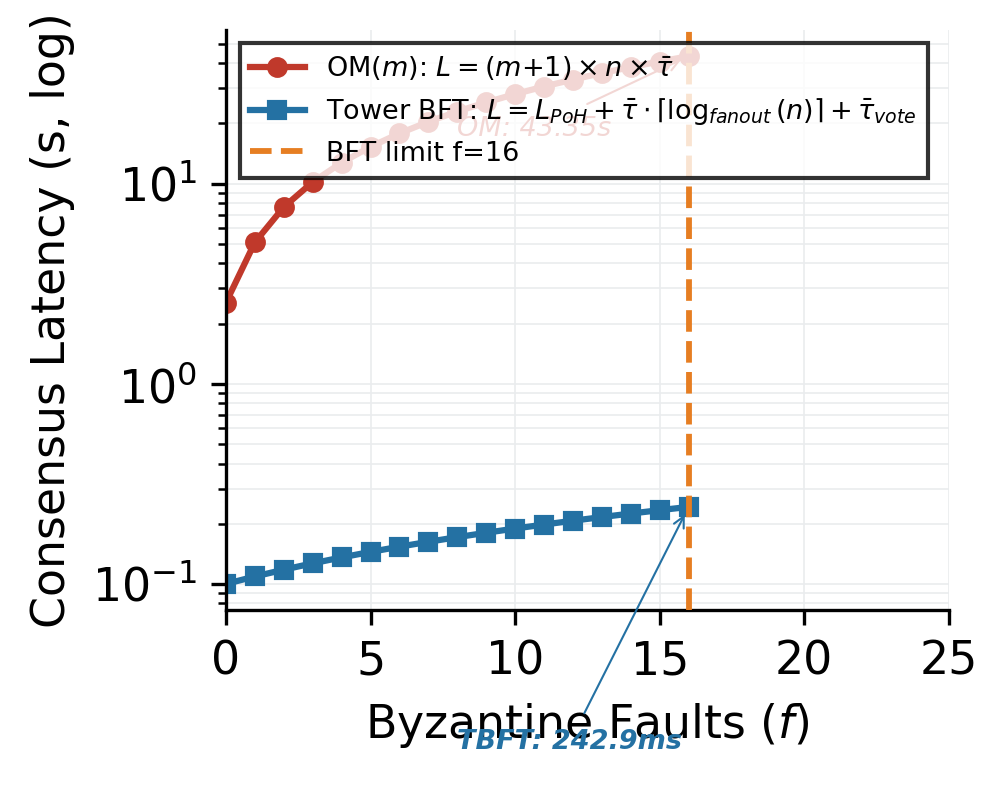
\includegraphics[width=0.75\textwidth]{figures/analytical_latency.png}
\end{figure}
\clearpage

\section{Analytical Latency Sensitivity}
\textbf{File:} \texttt{analytical\_latency\_sensitivity.png} \\
\textbf{Concept/Origin:} This plot visualizes \textbf{Analytical Latency Sensitivity Metric} as a function of \textbf{Time / Baseline Parameter}. \\
\textbf{Equations/Framework:} 
 L_{total} = L_{net} + L_{consensus} 
\vspace{0.5cm}
\begin{figure}[H]
    \centering
    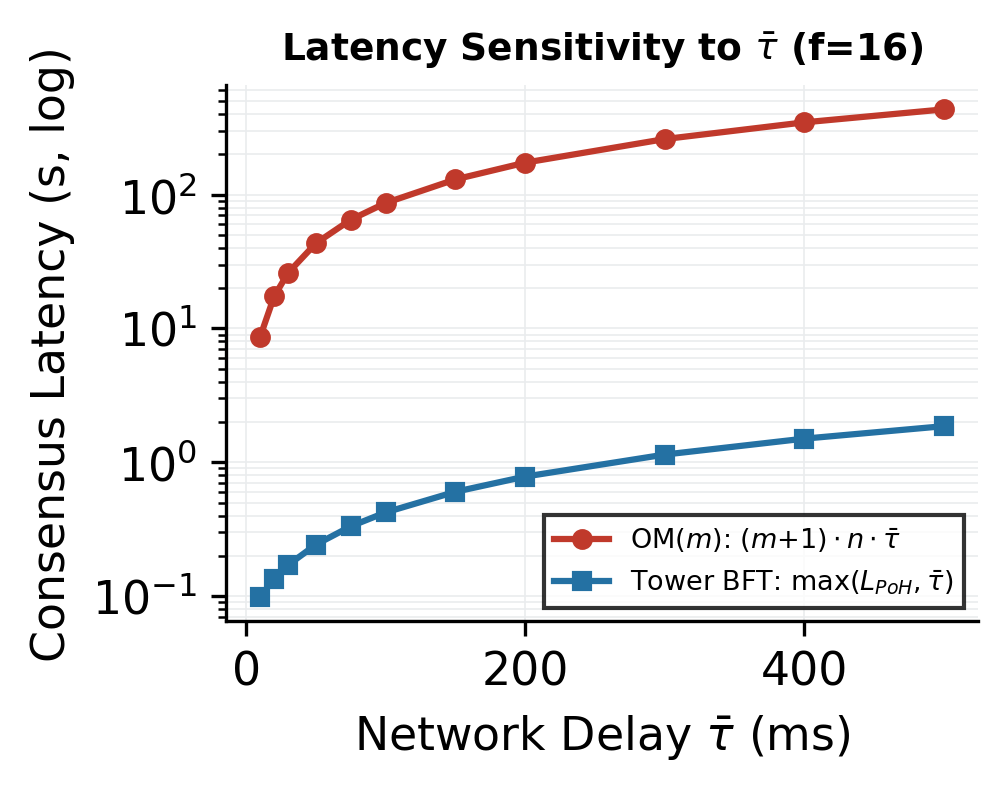
\includegraphics[width=0.75\textwidth]{figures/analytical_latency_sensitivity.png}
\end{figure}
\clearpage

\section{Analytical Probability Breakdown}
\textbf{File:} \texttt{analytical\_probability\_breakdown.png} \\
\textbf{Concept/Origin:} This plot visualizes \textbf{Analytical Probability Breakdown Metric} as a function of \textbf{Time / Baseline Parameter}. \\
\textbf{Equations/Framework:} 
 P_{Byz} = \sum_{i=f+1}^{n} \binom{n}{i} p_c^i (1-p_c)^{n-i} 
 P_{temporal} = 1 - e^{-\lambda L P_{TA}} 
\vspace{0.5cm}
\begin{figure}[H]
    \centering
    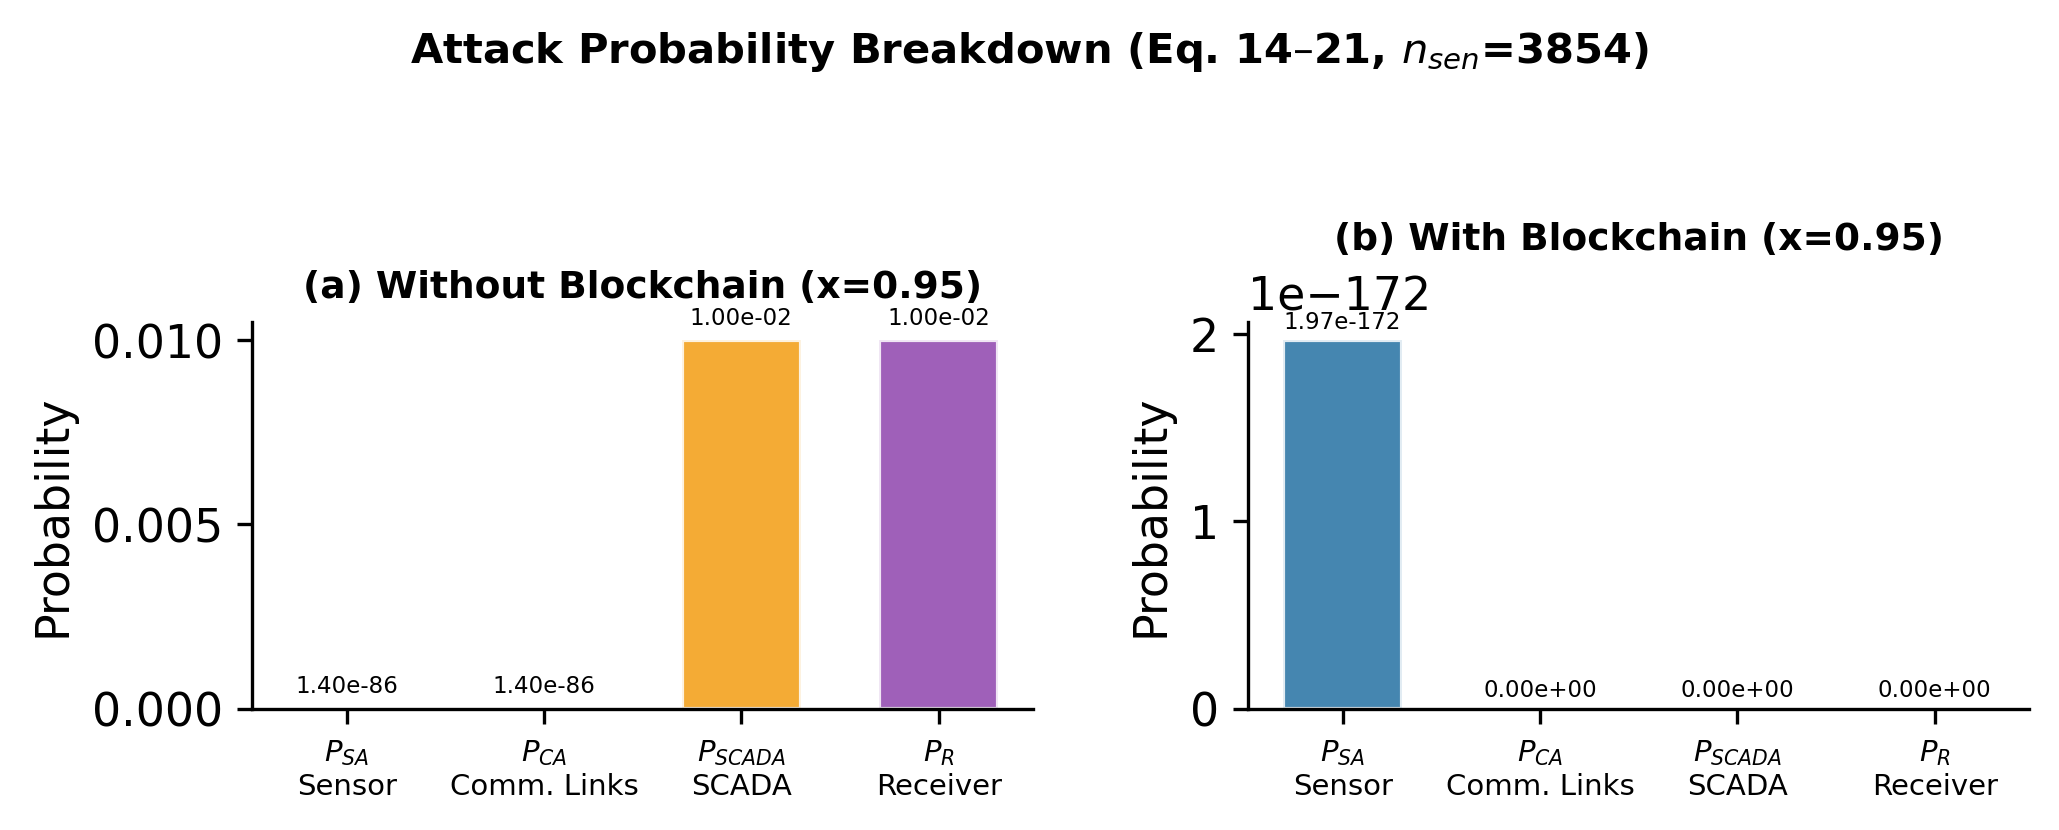
\includegraphics[width=0.75\textwidth]{figures/analytical_probability_breakdown.png}
\end{figure}
\clearpage

\section{Analytical Stsf Security}
\textbf{File:} \texttt{analytical\_stsf\_security.png} \\
\textbf{Concept/Origin:} This plot visualizes \textbf{Analytical Stsf Security Metric} as a function of \textbf{Time / Baseline Parameter}. \\
\textbf{Equations/Framework:} 
Empirical baseline calculation from simulation data.
\vspace{0.5cm}
\begin{figure}[H]
    \centering
    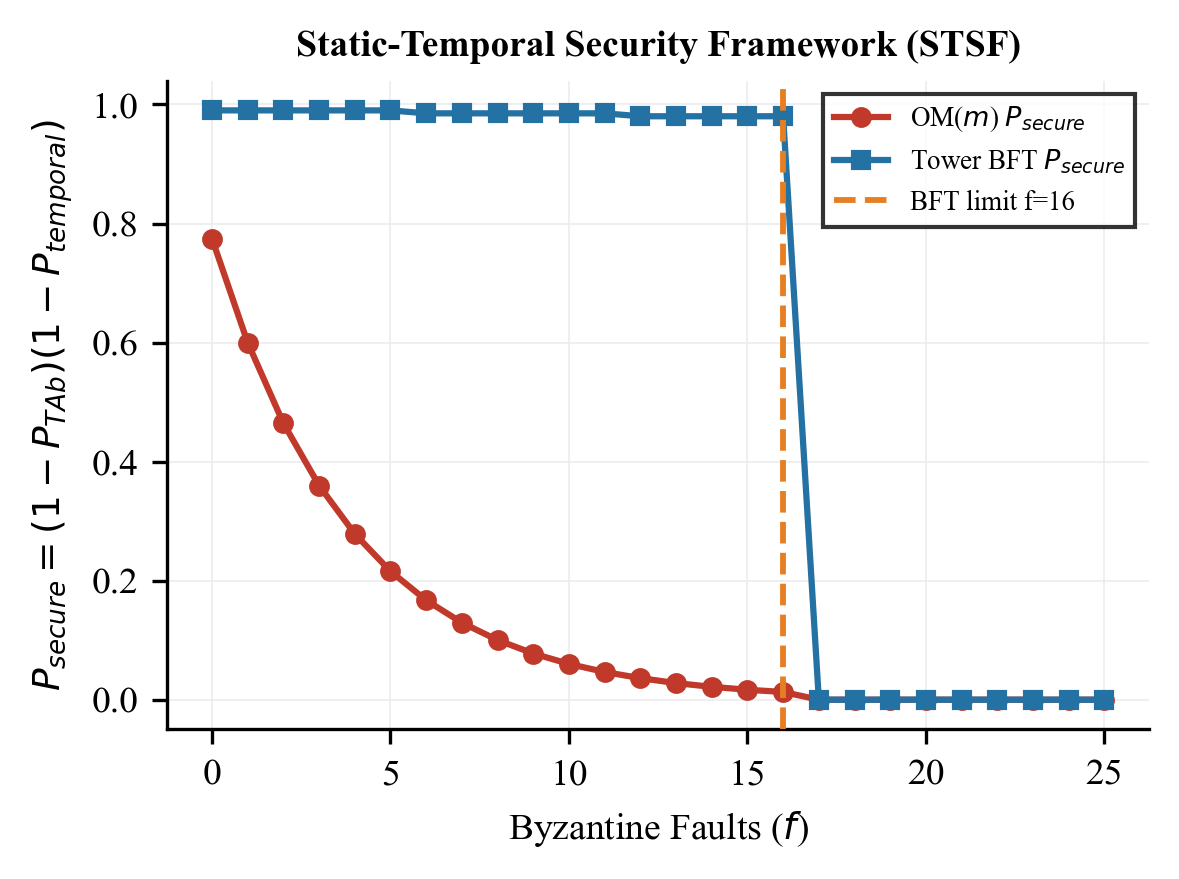
\includegraphics[width=0.75\textwidth]{figures/analytical_stsf_security.png}
\end{figure}
\clearpage

\section{Analytical Throughput}
\textbf{File:} \texttt{analytical\_throughput.png} \\
\textbf{Concept/Origin:} This plot visualizes \textbf{Analytical Throughput Metric} as a function of \textbf{Time / Baseline Parameter}. \\
\textbf{Equations/Framework:} 
Empirical baseline calculation from simulation data.
\vspace{0.5cm}
\begin{figure}[H]
    \centering
    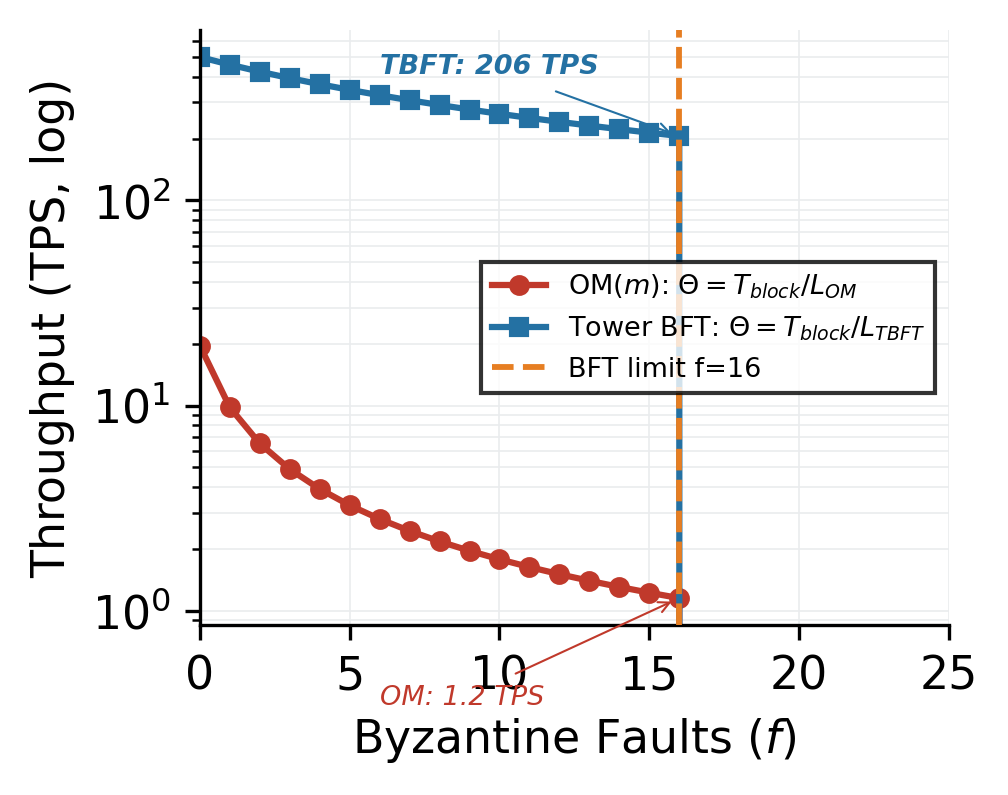
\includegraphics[width=0.75\textwidth]{figures/analytical_throughput.png}
\end{figure}
\clearpage

\section{Analytical Vulnerability}
\textbf{File:} \texttt{analytical\_vulnerability.png} \\
\textbf{Concept/Origin:} This plot visualizes \textbf{Analytical Vulnerability Metric} as a function of \textbf{Time / Baseline Parameter}. \\
\textbf{Equations/Framework:} 
 P_{Byz} = \sum_{i=f+1}^{n} \binom{n}{i} p_c^i (1-p_c)^{n-i} 
 P_{temporal} = 1 - e^{-\lambda L P_{TA}} 
\vspace{0.5cm}
\begin{figure}[H]
    \centering
    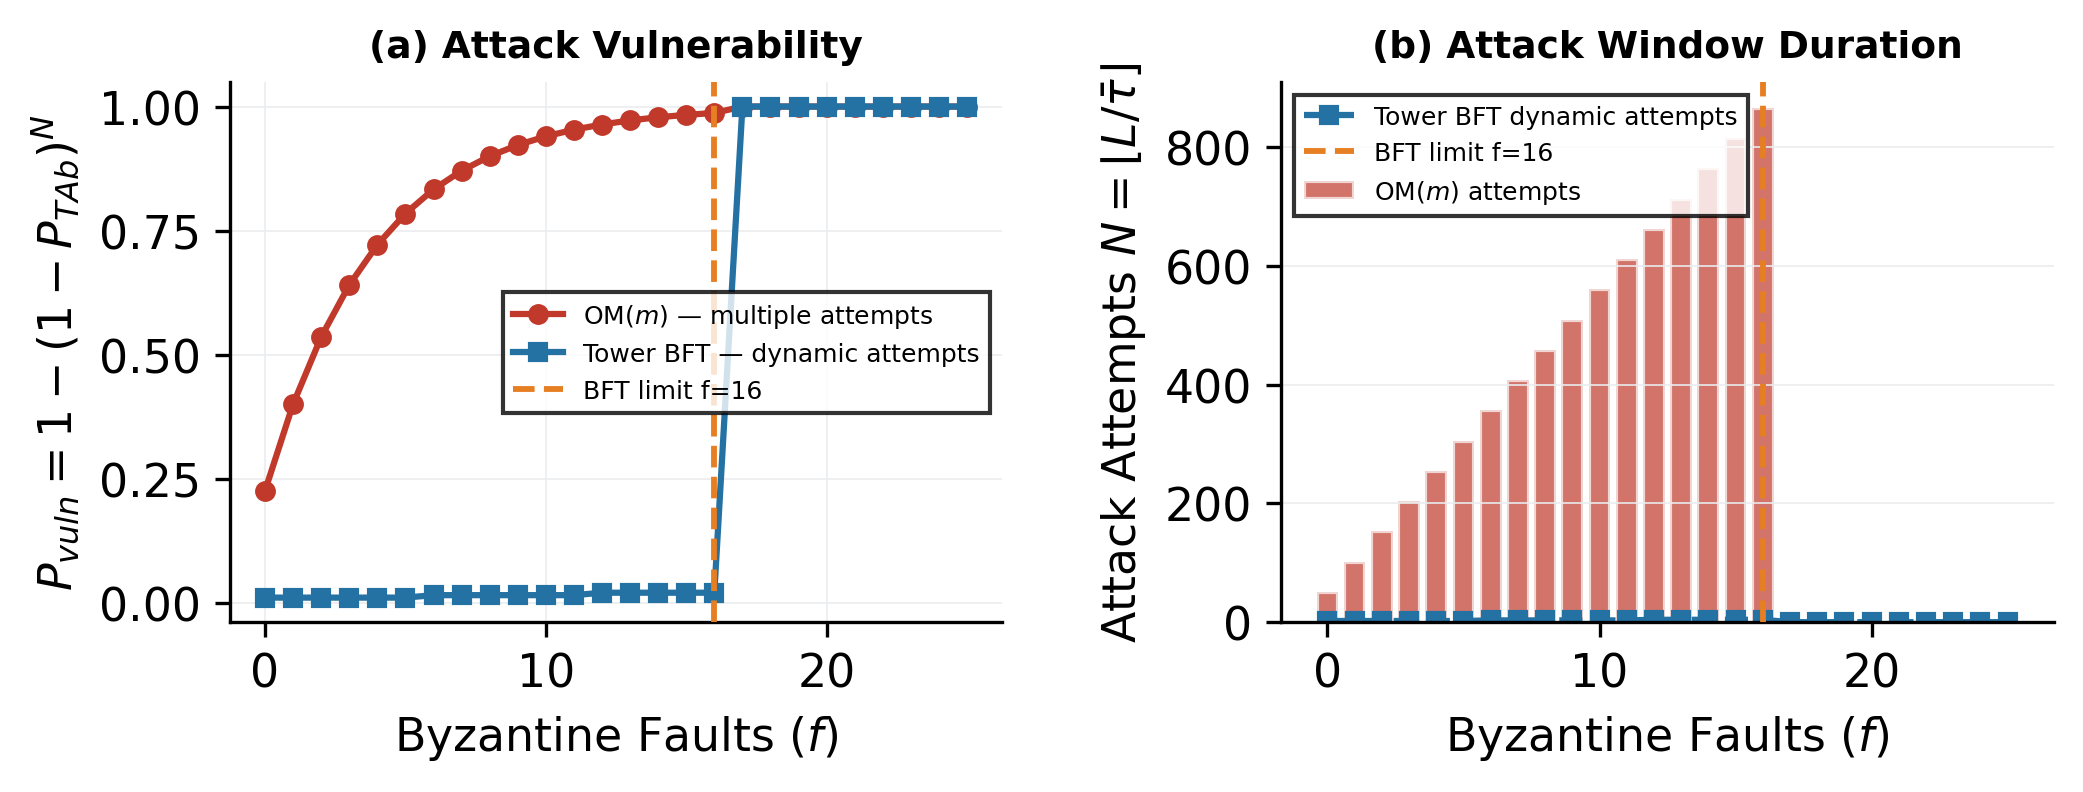
\includegraphics[width=0.75\textwidth]{figures/analytical_vulnerability.png}
\end{figure}
\clearpage

\section{Comparison Attack Window}
\textbf{File:} \texttt{comparison\_attack\_window.png} \\
\textbf{Concept/Origin:} This plot visualizes \textbf{Comparison Attack Window Metric} as a function of \textbf{Time / Baseline Parameter}. \\
\textbf{Equations/Framework:} 
Empirical baseline calculation from simulation data.
\vspace{0.5cm}
\begin{figure}[H]
    \centering
    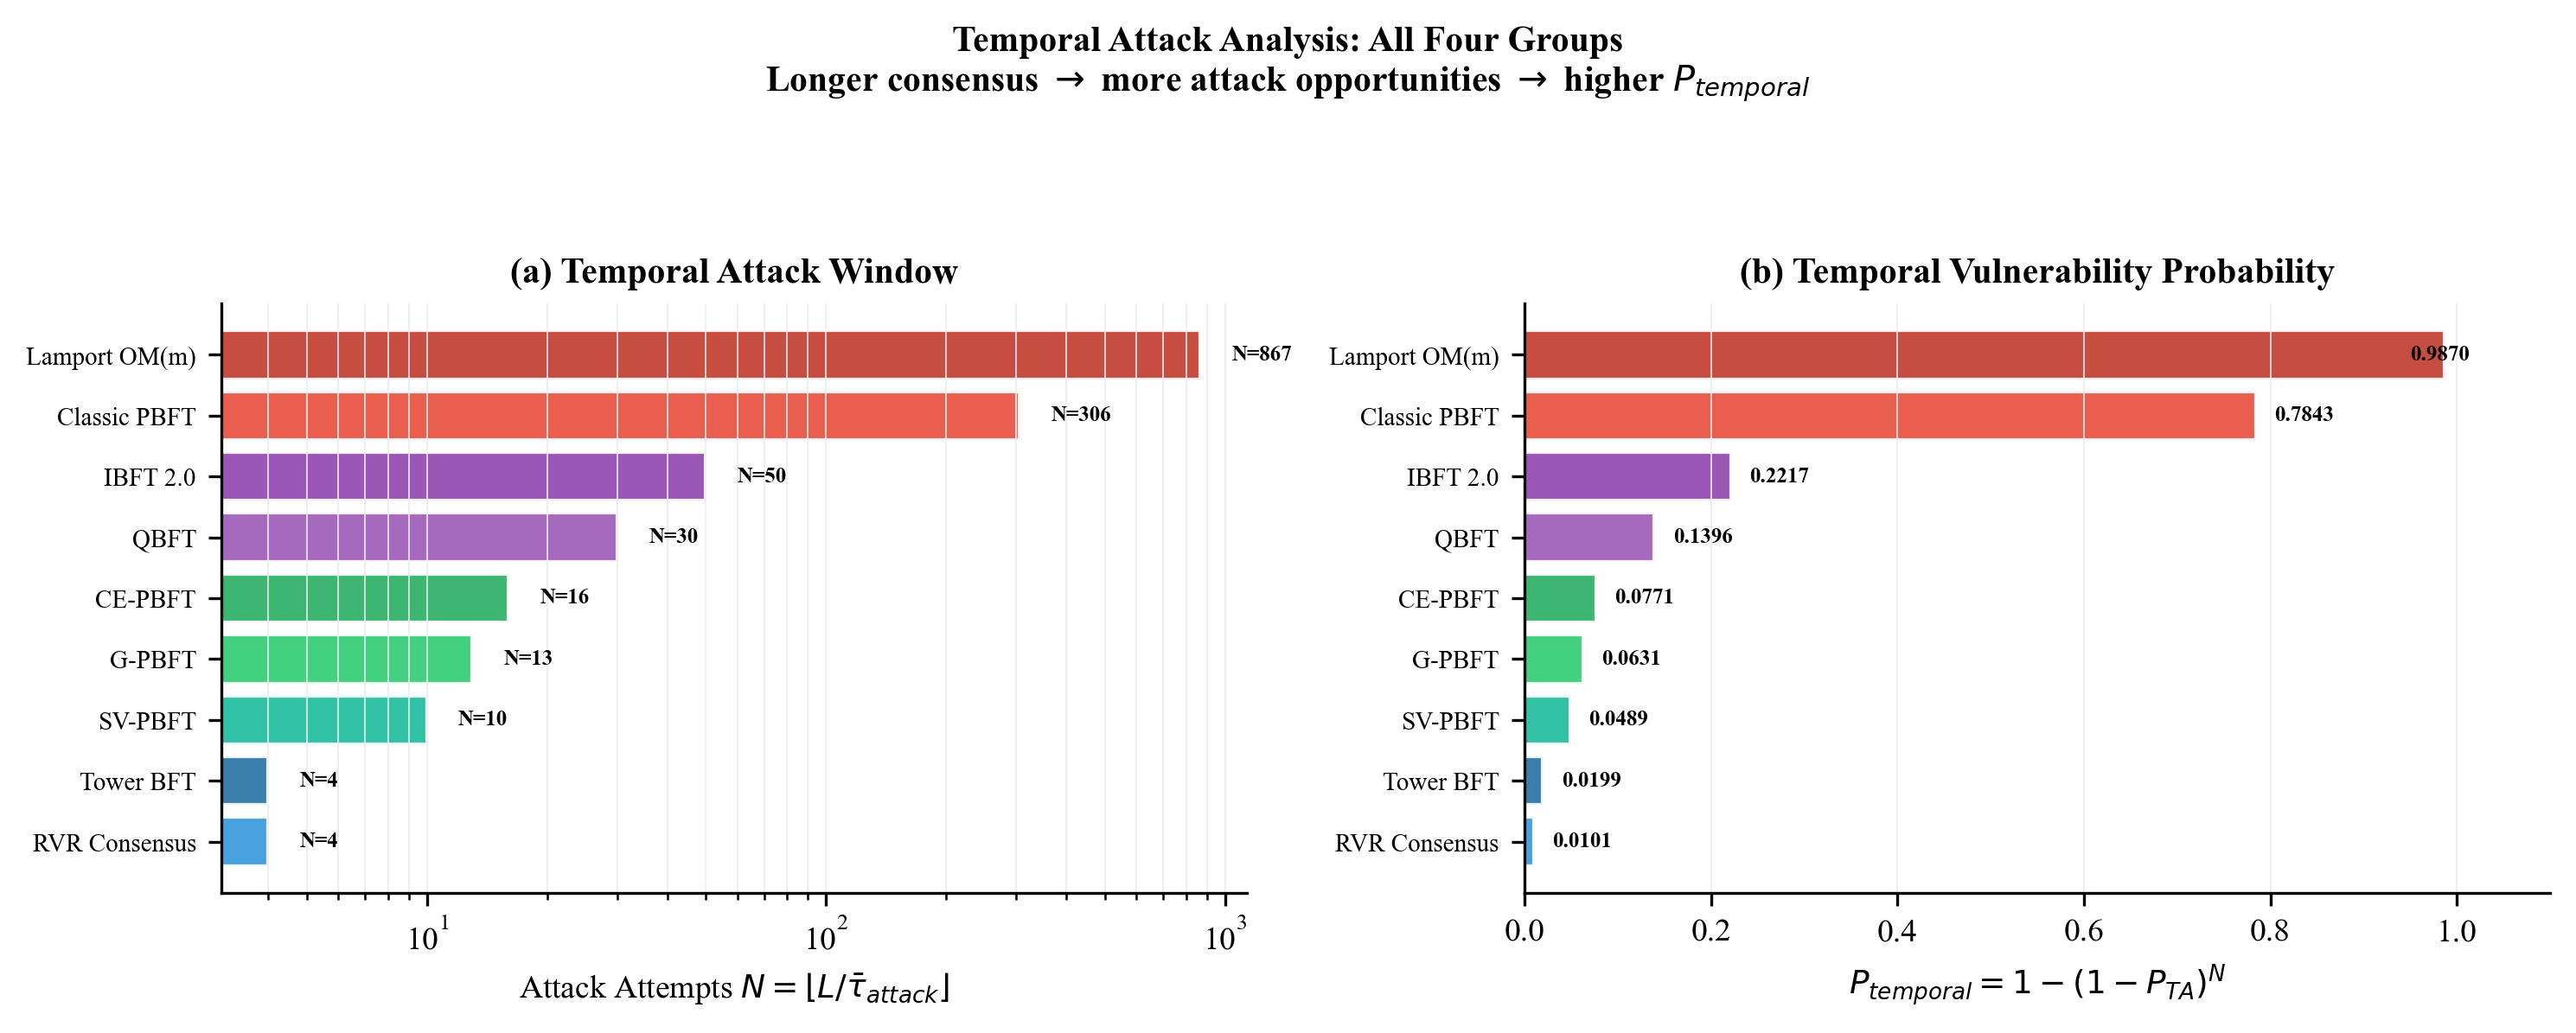
\includegraphics[width=0.75\textwidth]{figures/comparison_attack_window.png}
\end{figure}
\clearpage

\section{Comparison Heatmap}
\textbf{File:} \texttt{comparison\_heatmap.png} \\
\textbf{Concept/Origin:} This plot visualizes \textbf{Comparison Heatmap Metric} as a function of \textbf{Time / Baseline Parameter}. \\
\textbf{Equations/Framework:} 
 P_{secure} = \max( \text{Security} ) \quad \text{s.t.} \quad L_{total} \le L_{max} 
\vspace{0.5cm}
\begin{figure}[H]
    \centering
    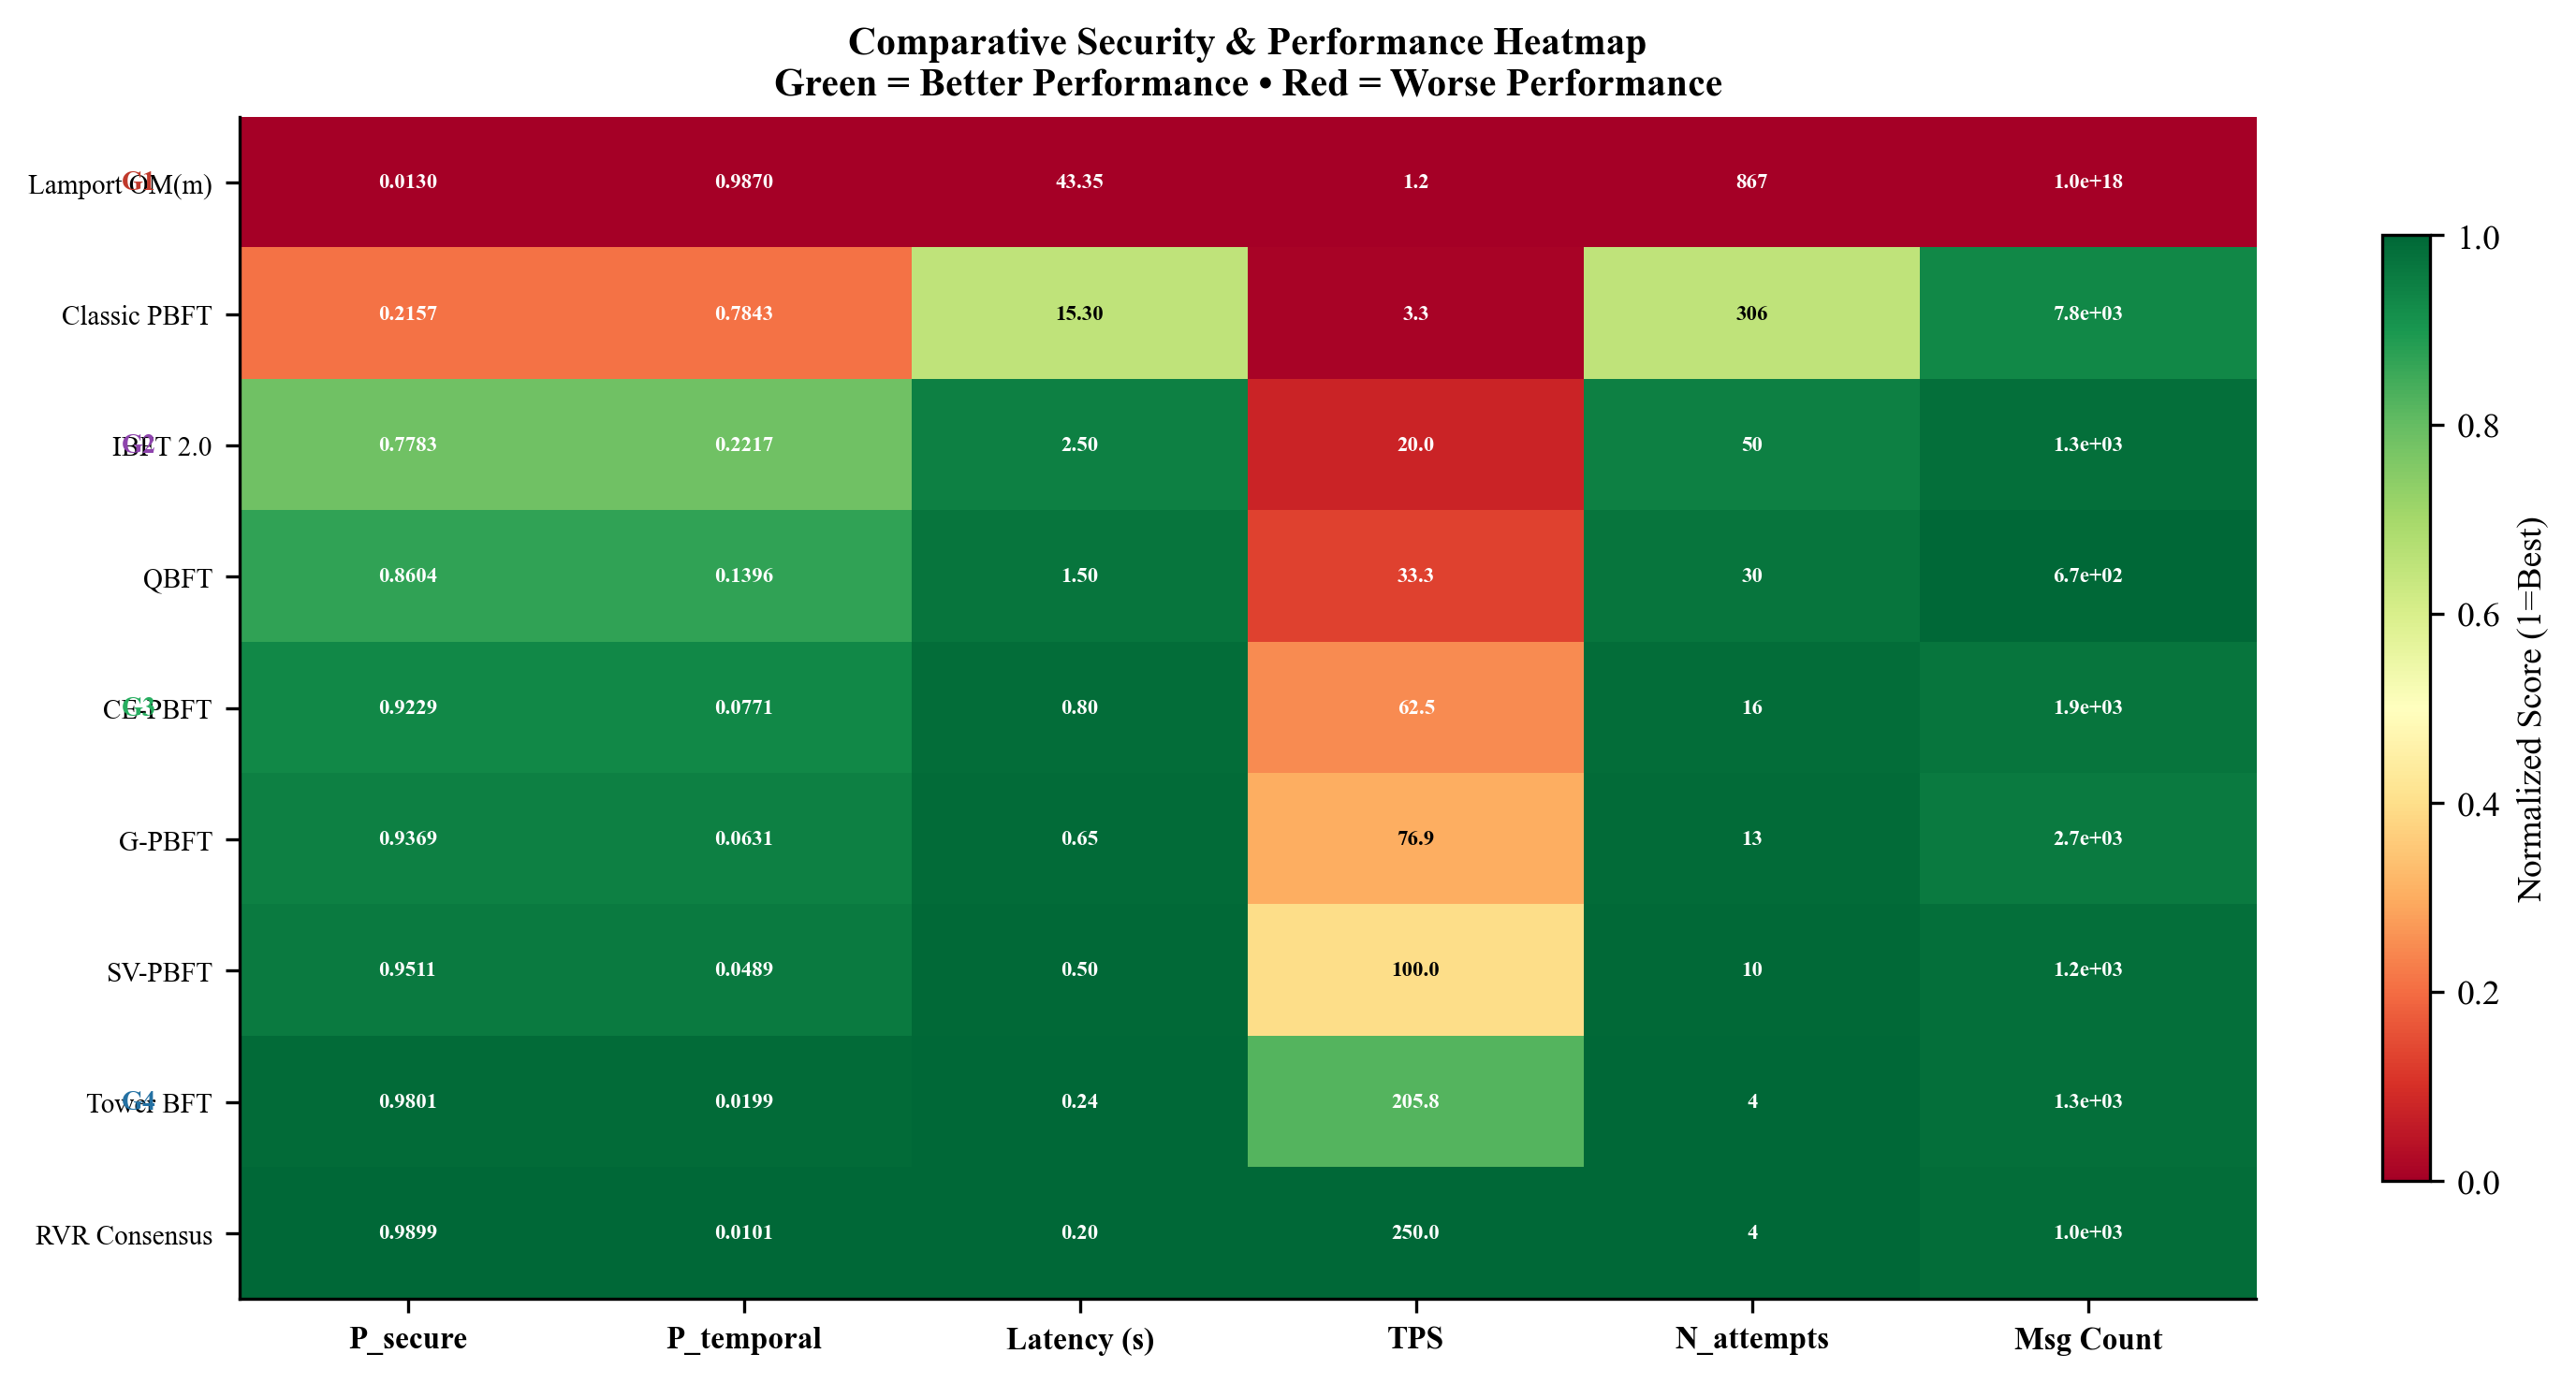
\includegraphics[width=0.75\textwidth]{figures/comparison_heatmap.png}
\end{figure}
\clearpage

\section{Comparison Latency Log}
\textbf{File:} \texttt{comparison\_latency\_log.png} \\
\textbf{Concept/Origin:} This plot visualizes \textbf{Comparison Latency Log Metric} as a function of \textbf{Time / Baseline Parameter}. \\
\textbf{Equations/Framework:} 
 L_{total} = L_{net} + L_{consensus} 
\vspace{0.5cm}
\begin{figure}[H]
    \centering
    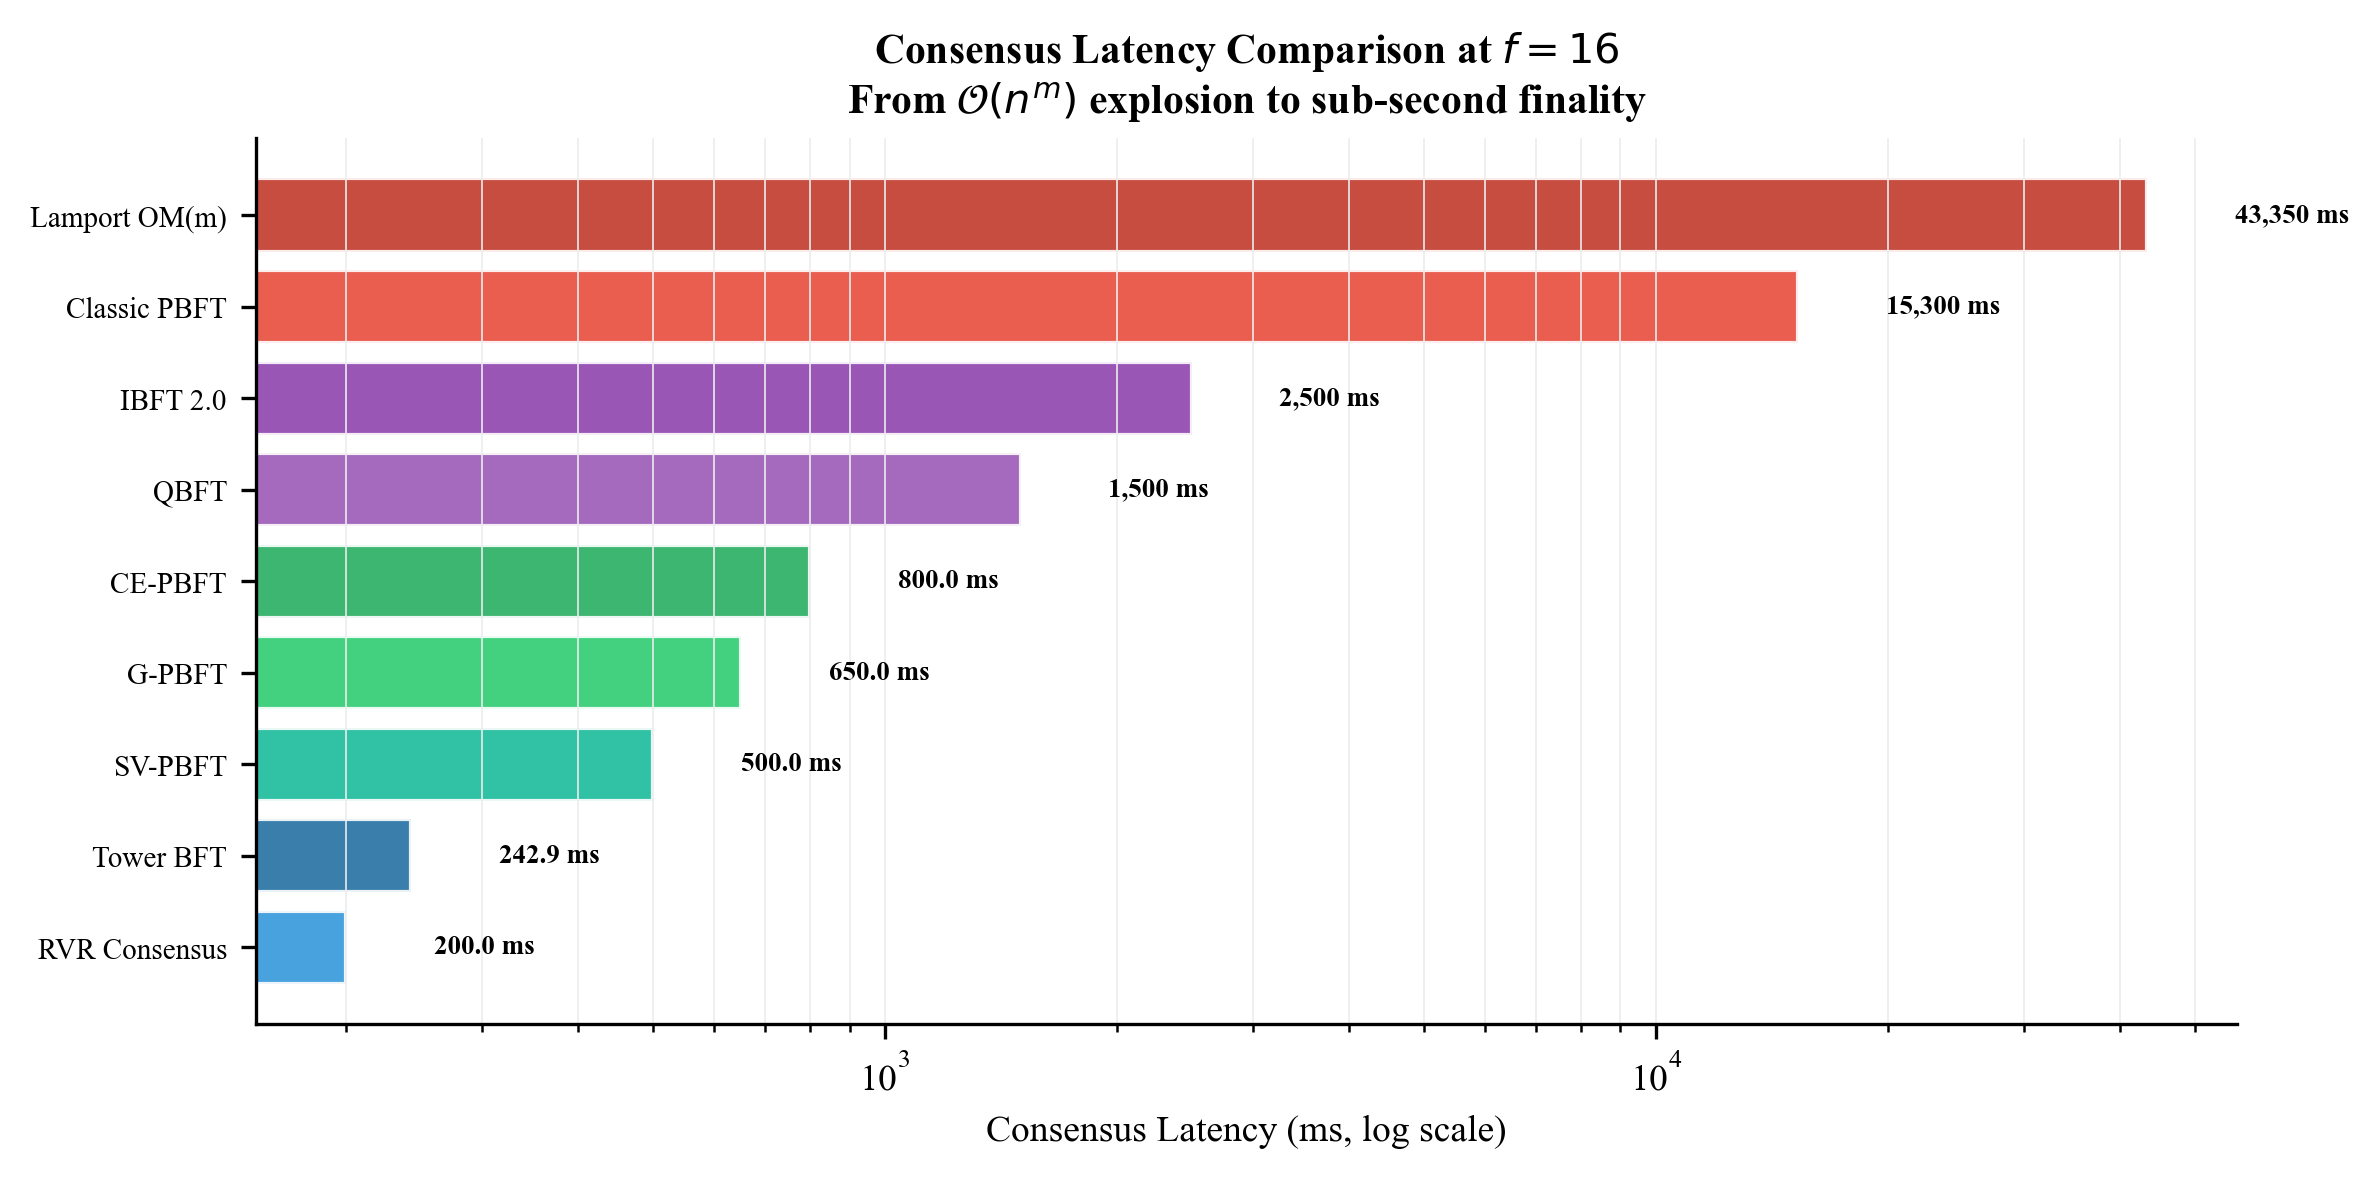
\includegraphics[width=0.75\textwidth]{figures/comparison_latency_log.png}
\end{figure}
\clearpage

\section{Comparison Message Complexity}
\textbf{File:} \texttt{comparison\_message\_complexity.png} \\
\textbf{Concept/Origin:} This plot visualizes \textbf{Comparison Message Complexity Metric} as a function of \textbf{Time / Baseline Parameter}. \\
\textbf{Equations/Framework:} 
 E_{total} = E_{tx} + E_{rx} + E_{crypto} 
\vspace{0.5cm}
\begin{figure}[H]
    \centering
    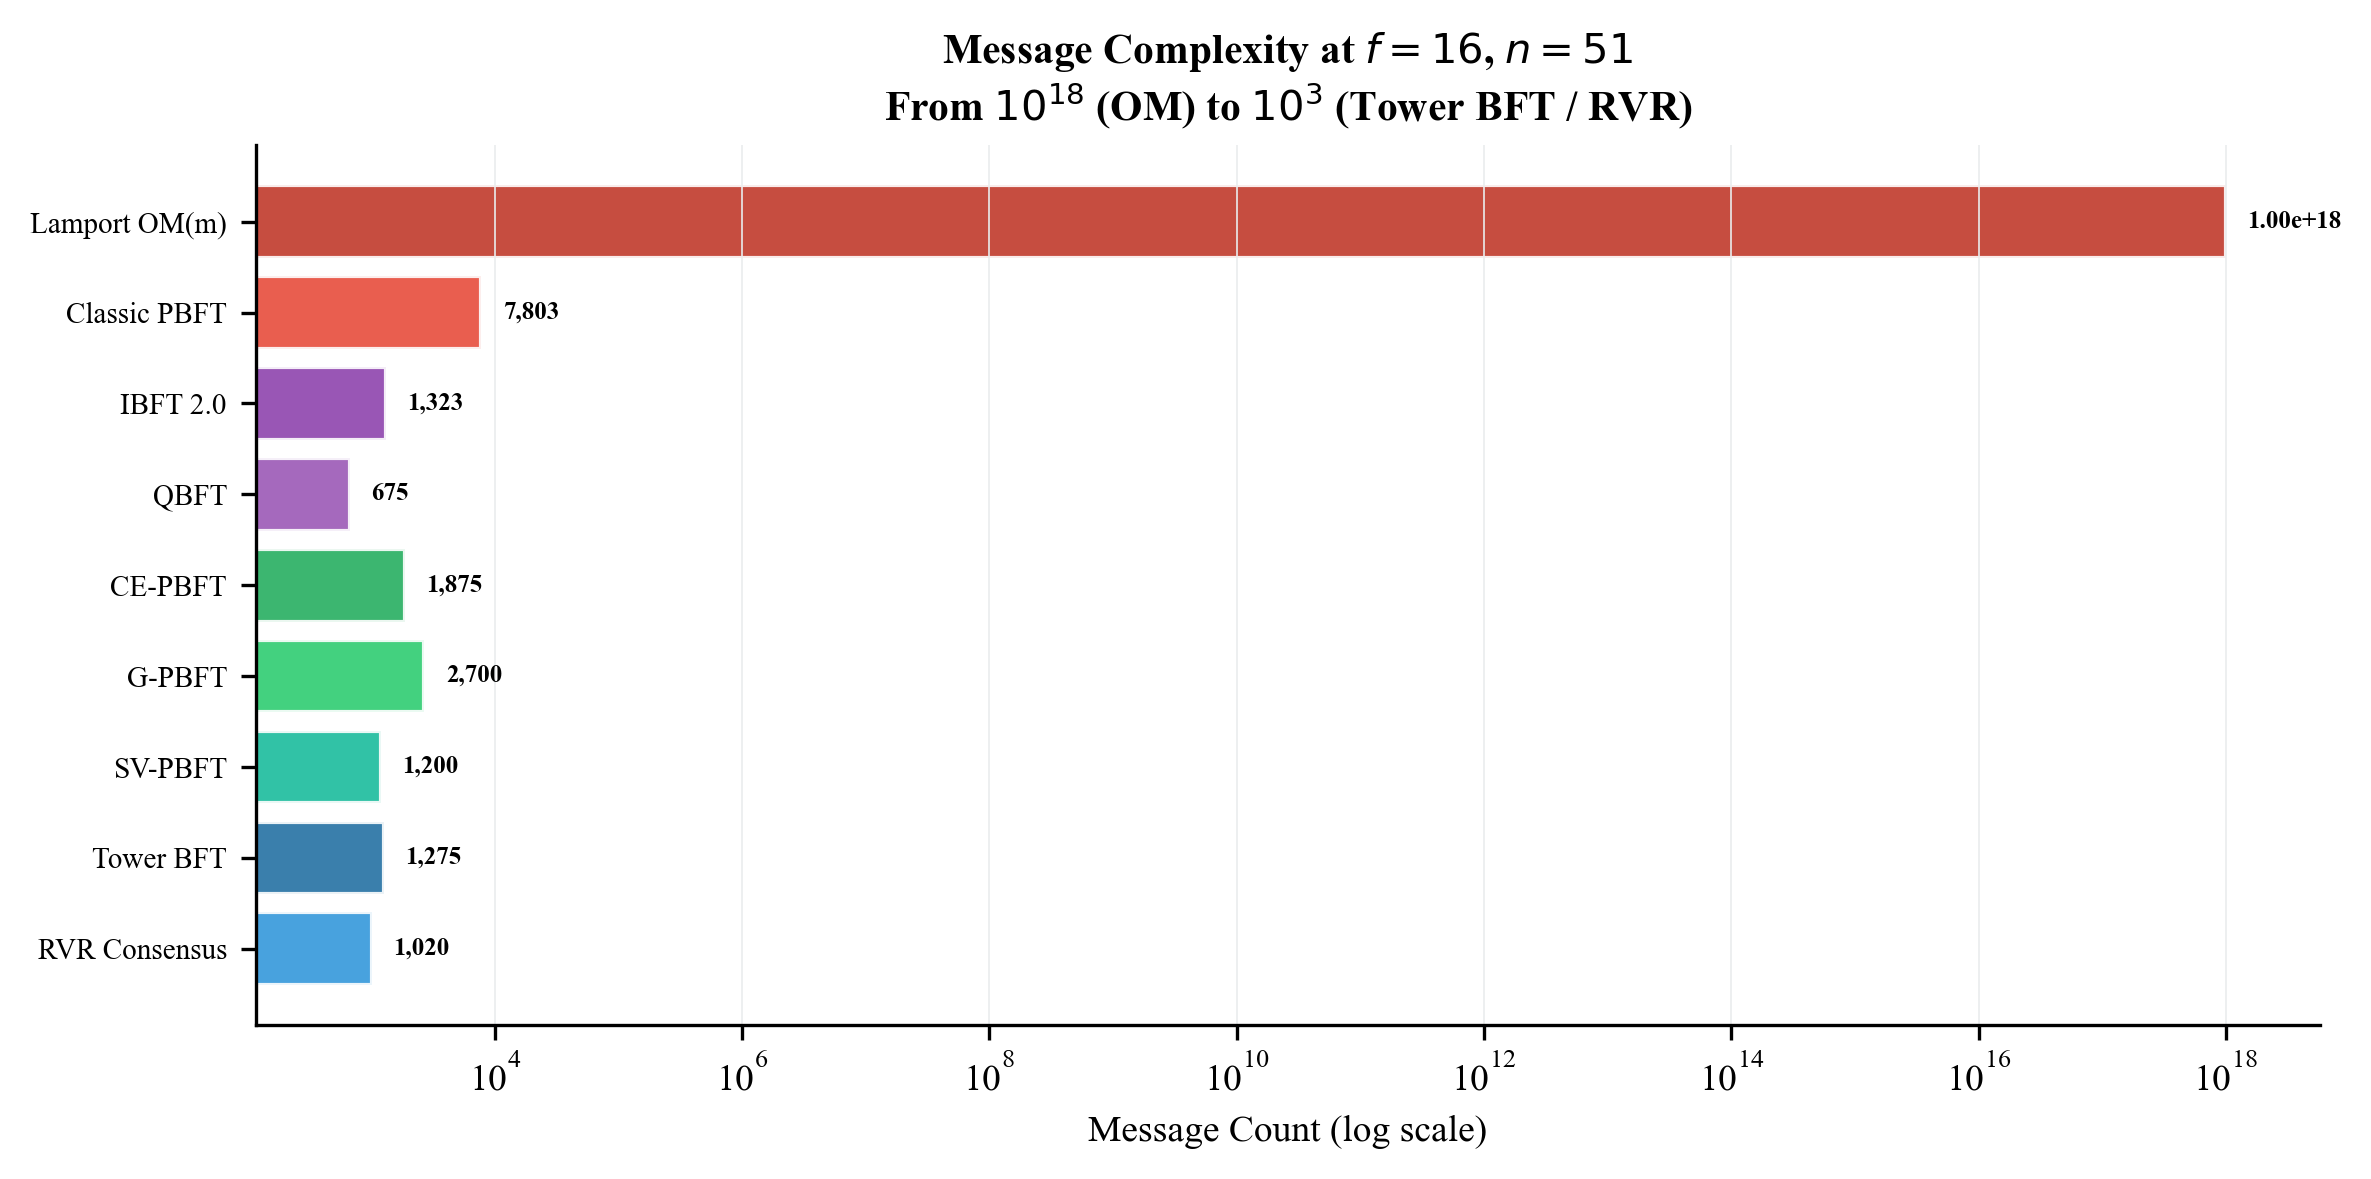
\includegraphics[width=0.75\textwidth]{figures/comparison_message_complexity.png}
\end{figure}
\clearpage

\section{Comparison Psecure Bar}
\textbf{File:} \texttt{comparison\_psecure\_bar.png} \\
\textbf{Concept/Origin:} This plot visualizes \textbf{Comparison Psecure Bar Metric} as a function of \textbf{Time / Baseline Parameter}. \\
\textbf{Equations/Framework:} 
 P_{Byz} = \sum_{i=f+1}^{n} \binom{n}{i} p_c^i (1-p_c)^{n-i} 
 P_{temporal} = 1 - e^{-\lambda L P_{TA}} 
\vspace{0.5cm}
\begin{figure}[H]
    \centering
    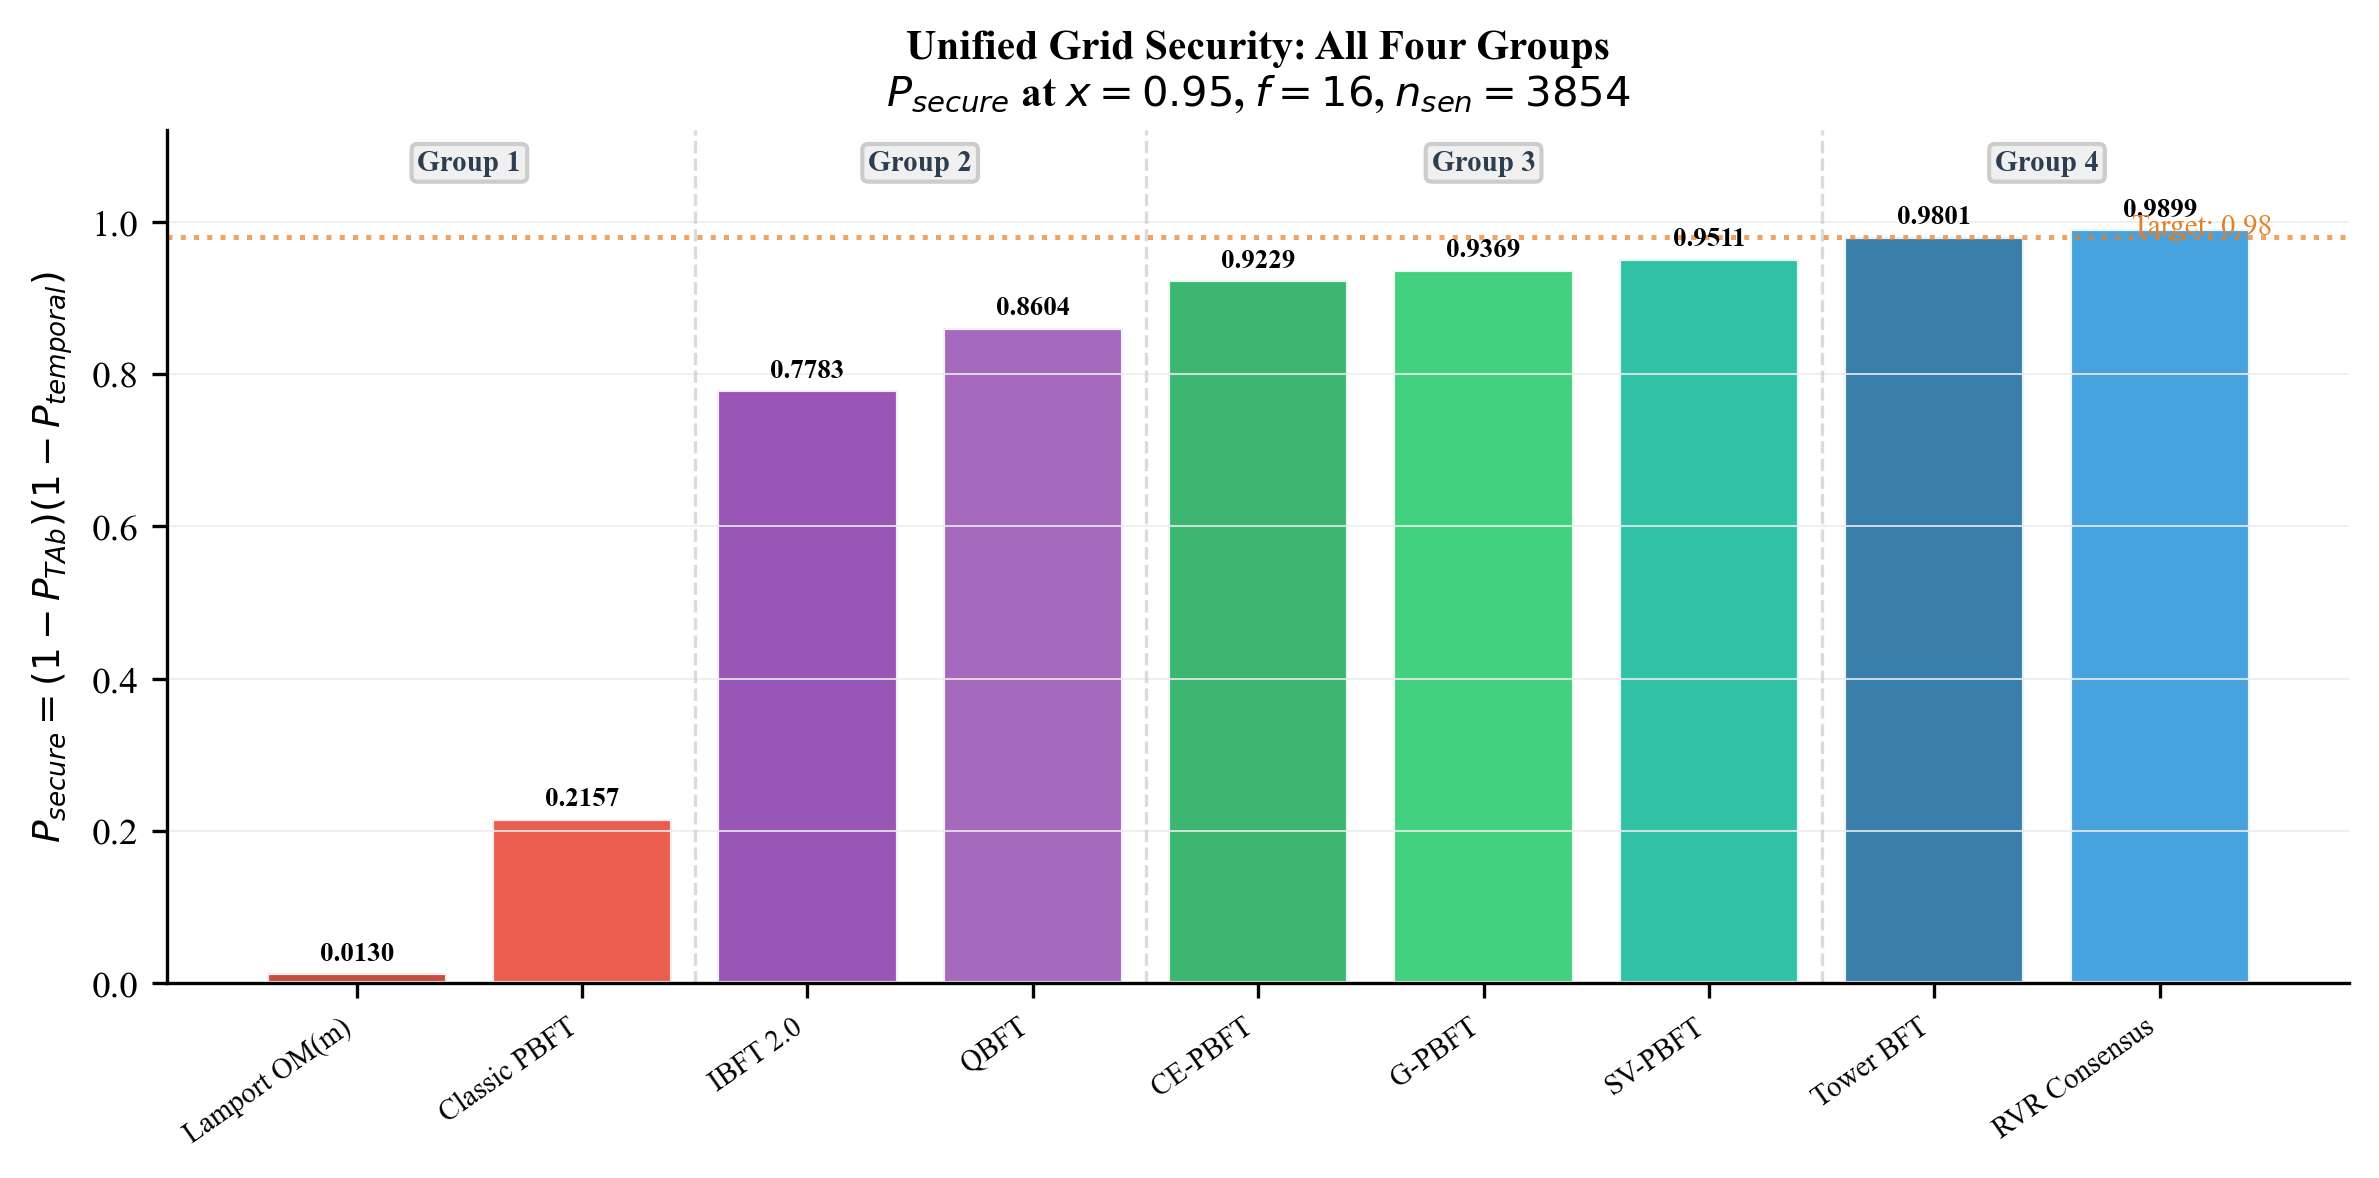
\includegraphics[width=0.75\textwidth]{figures/comparison_psecure_bar.png}
\end{figure}
\clearpage

\section{Comparison Radar}
\textbf{File:} \texttt{comparison\_radar.png} \\
\textbf{Concept/Origin:} This plot visualizes \textbf{Comparison Radar Metric} as a function of \textbf{Time / Baseline Parameter}. \\
\textbf{Equations/Framework:} 
Empirical baseline calculation from simulation data.
\vspace{0.5cm}
\begin{figure}[H]
    \centering
    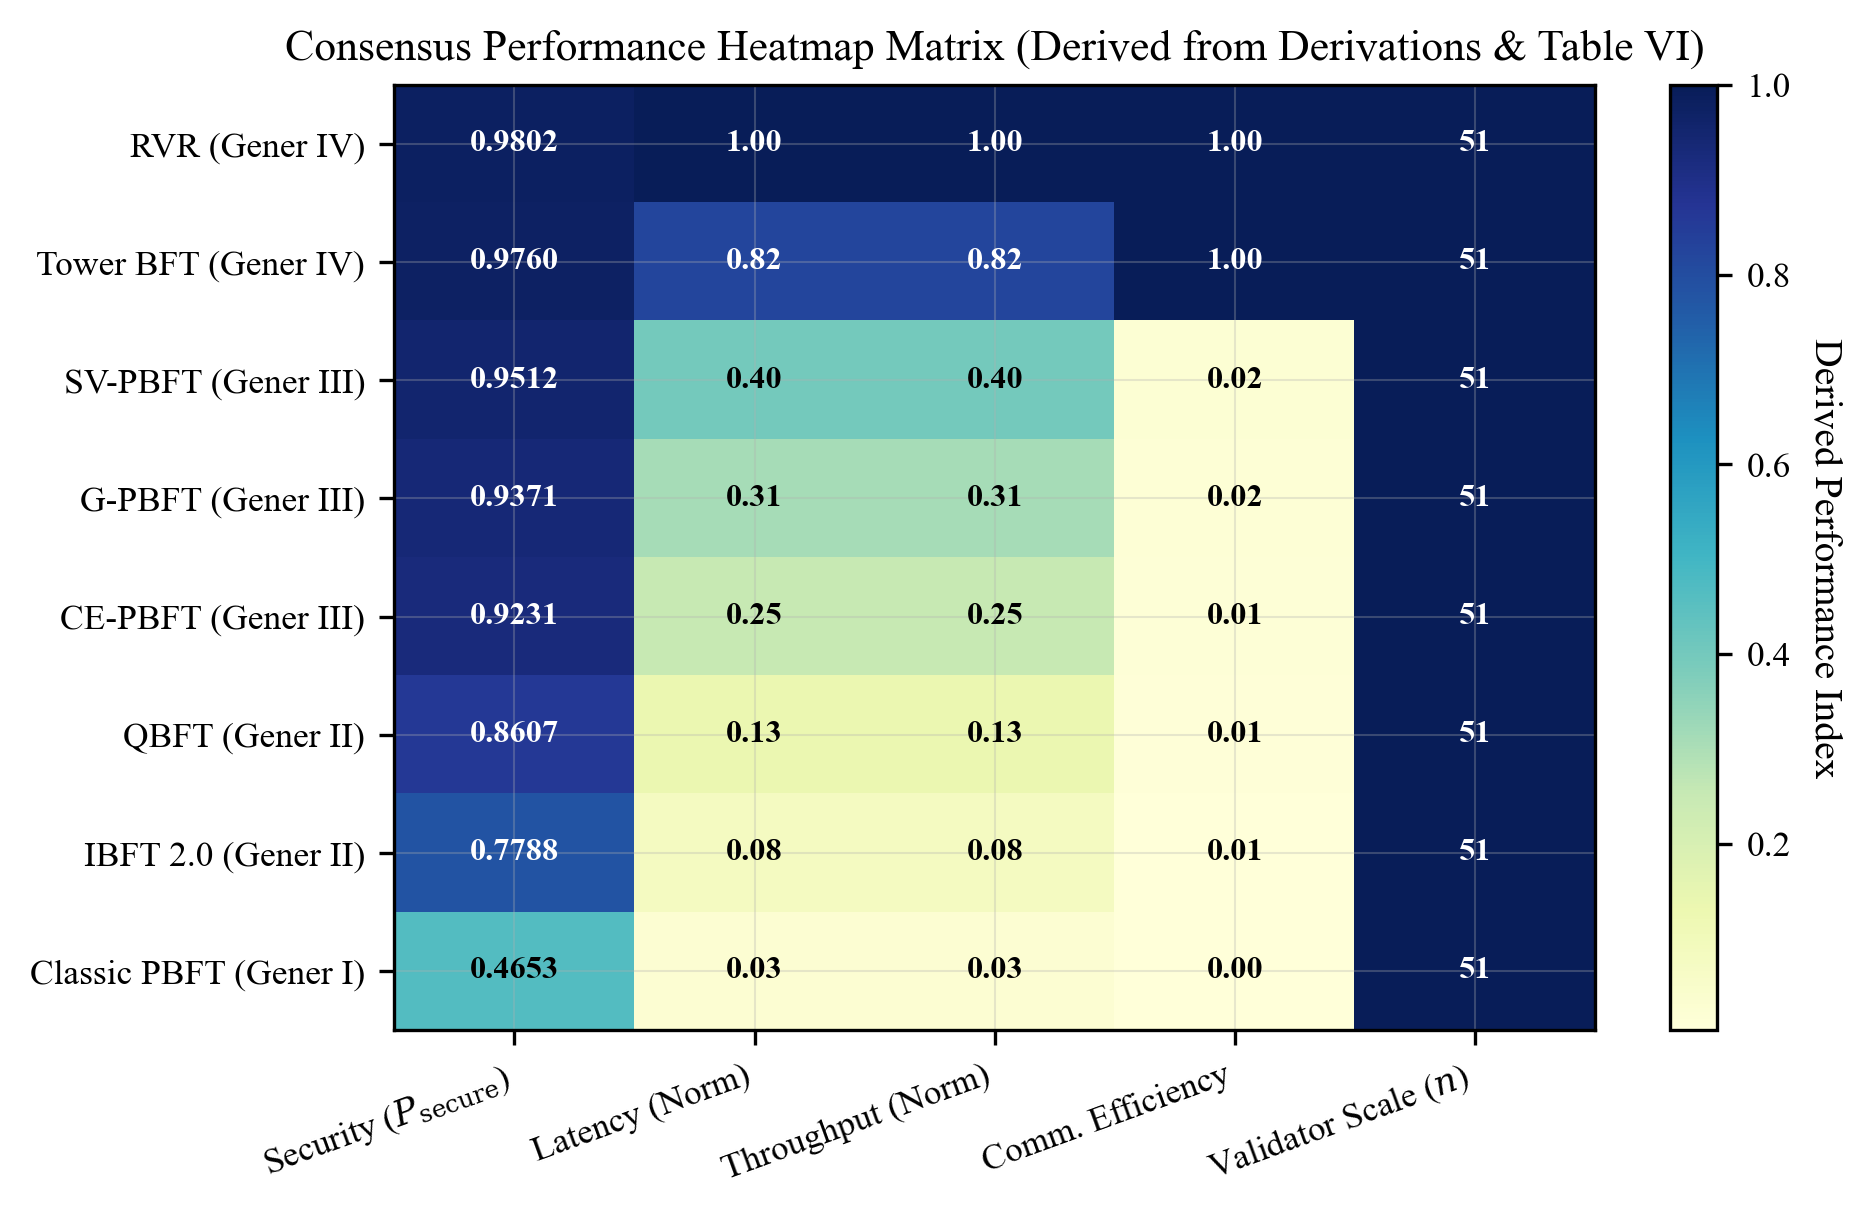
\includegraphics[width=0.75\textwidth]{figures/comparison_radar.png}
\end{figure}
\clearpage

\section{Comparison Temporal Decay}
\textbf{File:} \texttt{comparison\_temporal\_decay.png} \\
\textbf{Concept/Origin:} This plot visualizes \textbf{Comparison Temporal Decay Metric} as a function of \textbf{Time / Baseline Parameter}. \\
\textbf{Equations/Framework:} 
Empirical baseline calculation from simulation data.
\vspace{0.5cm}
\begin{figure}[H]
    \centering
    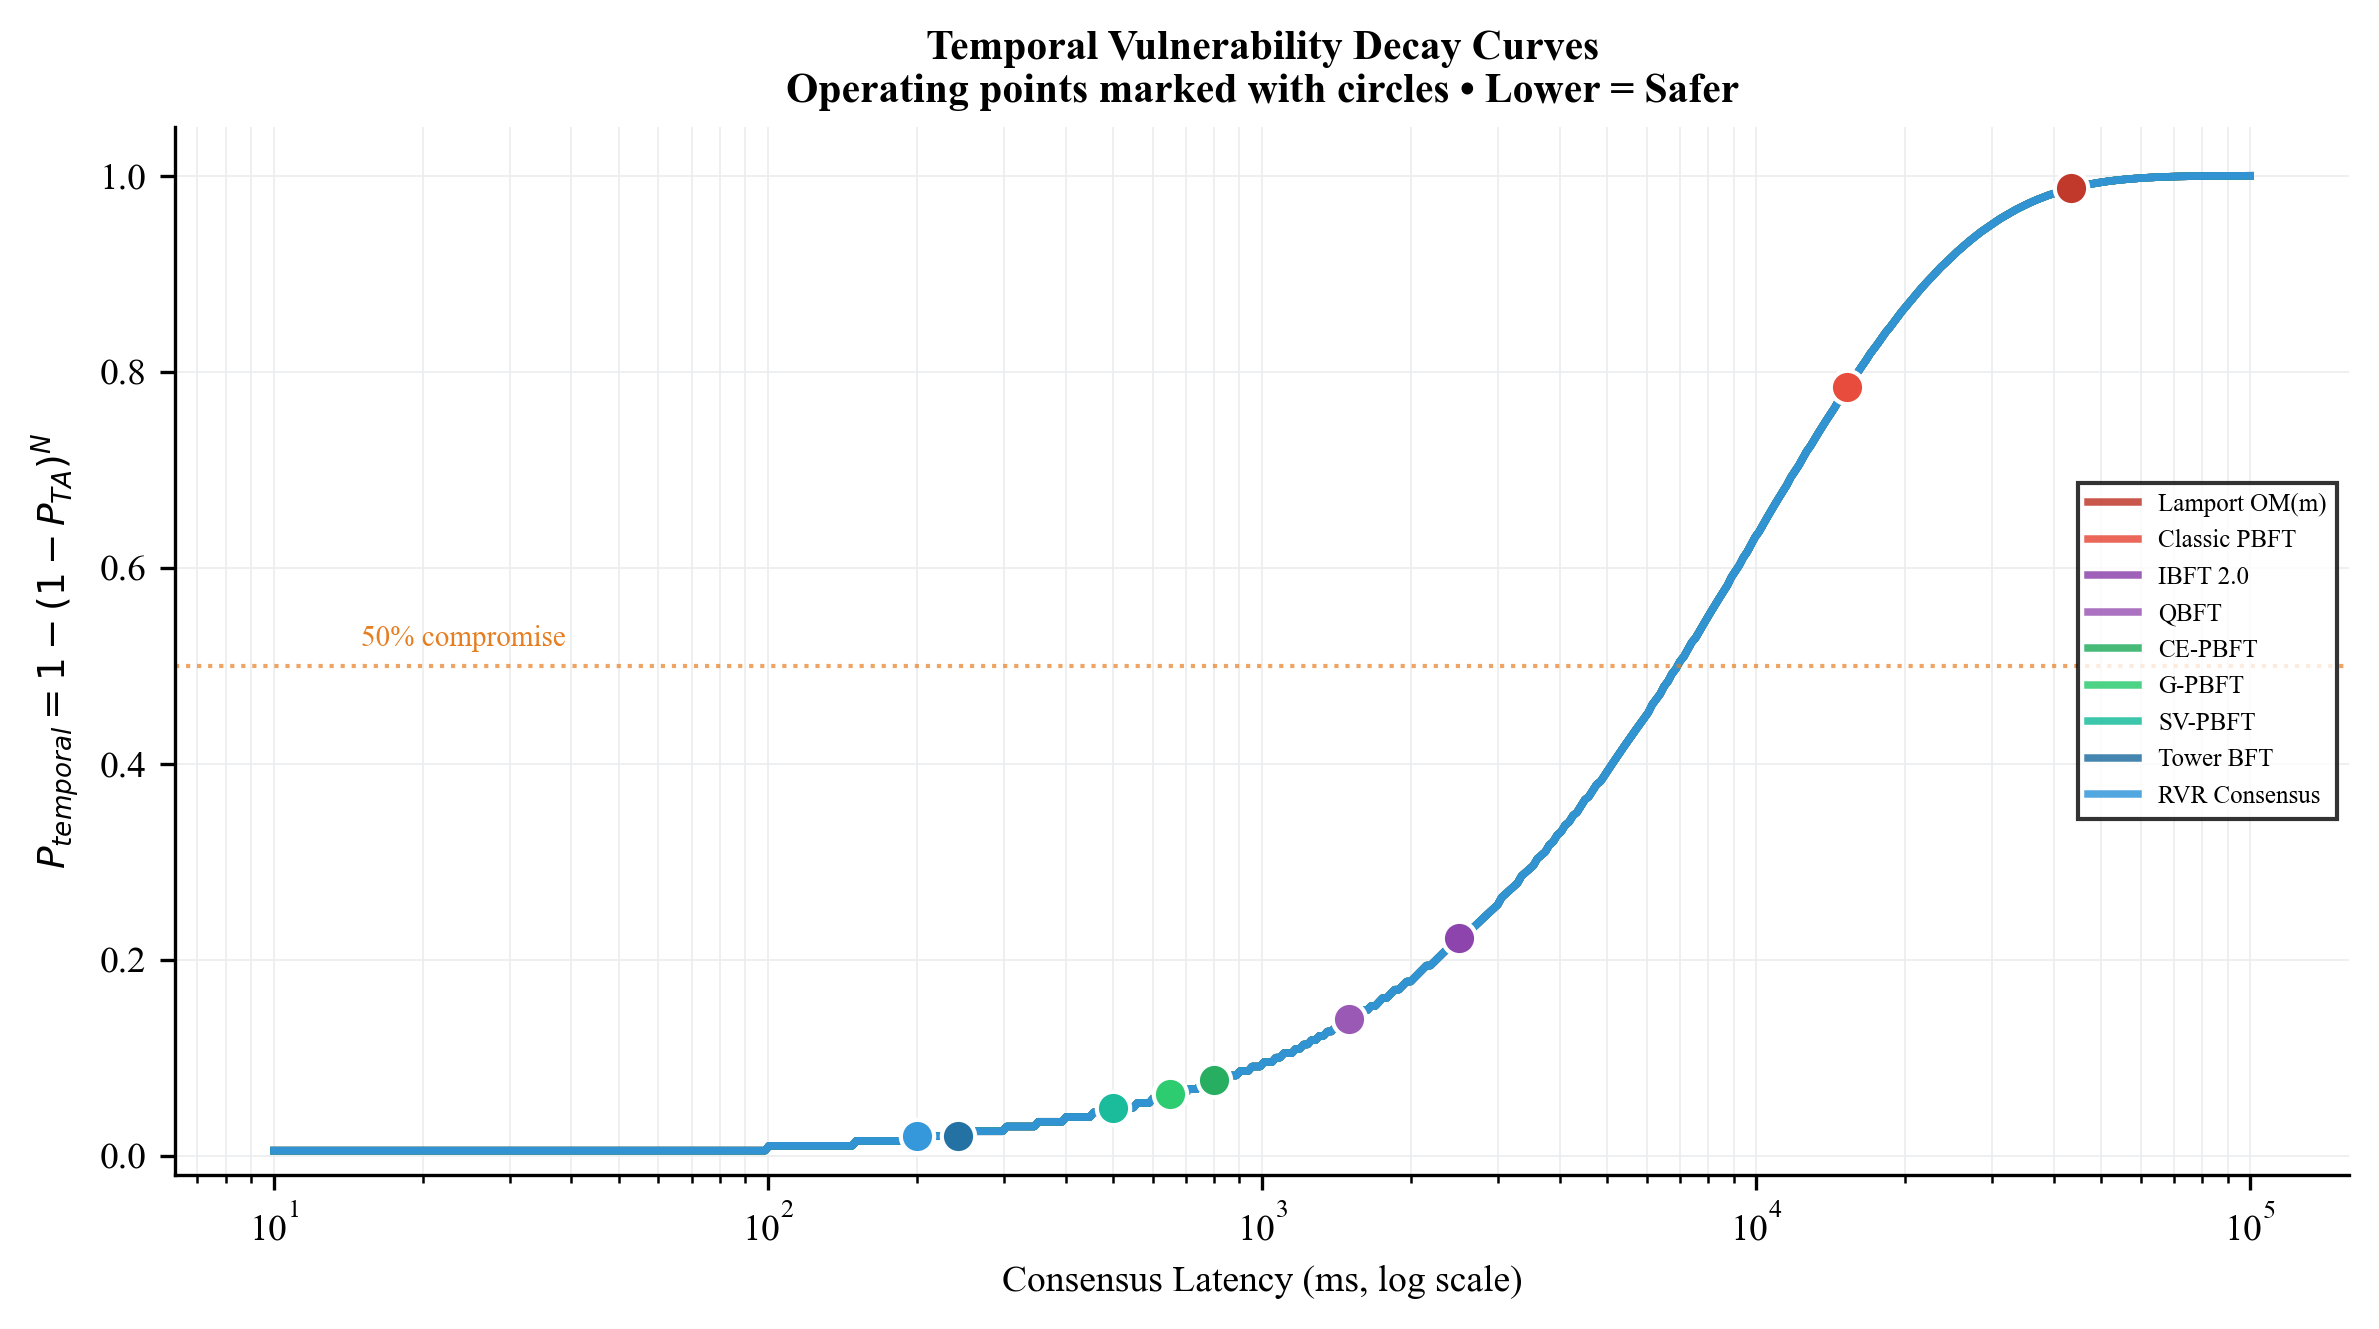
\includegraphics[width=0.75\textwidth]{figures/comparison_temporal_decay.png}
\end{figure}
\clearpage

\section{Comparison Throughput}
\textbf{File:} \texttt{comparison\_throughput.png} \\
\textbf{Concept/Origin:} This plot visualizes \textbf{Comparison Throughput Metric} as a function of \textbf{Time / Baseline Parameter}. \\
\textbf{Equations/Framework:} 
Empirical baseline calculation from simulation data.
\vspace{0.5cm}
\begin{figure}[H]
    \centering
    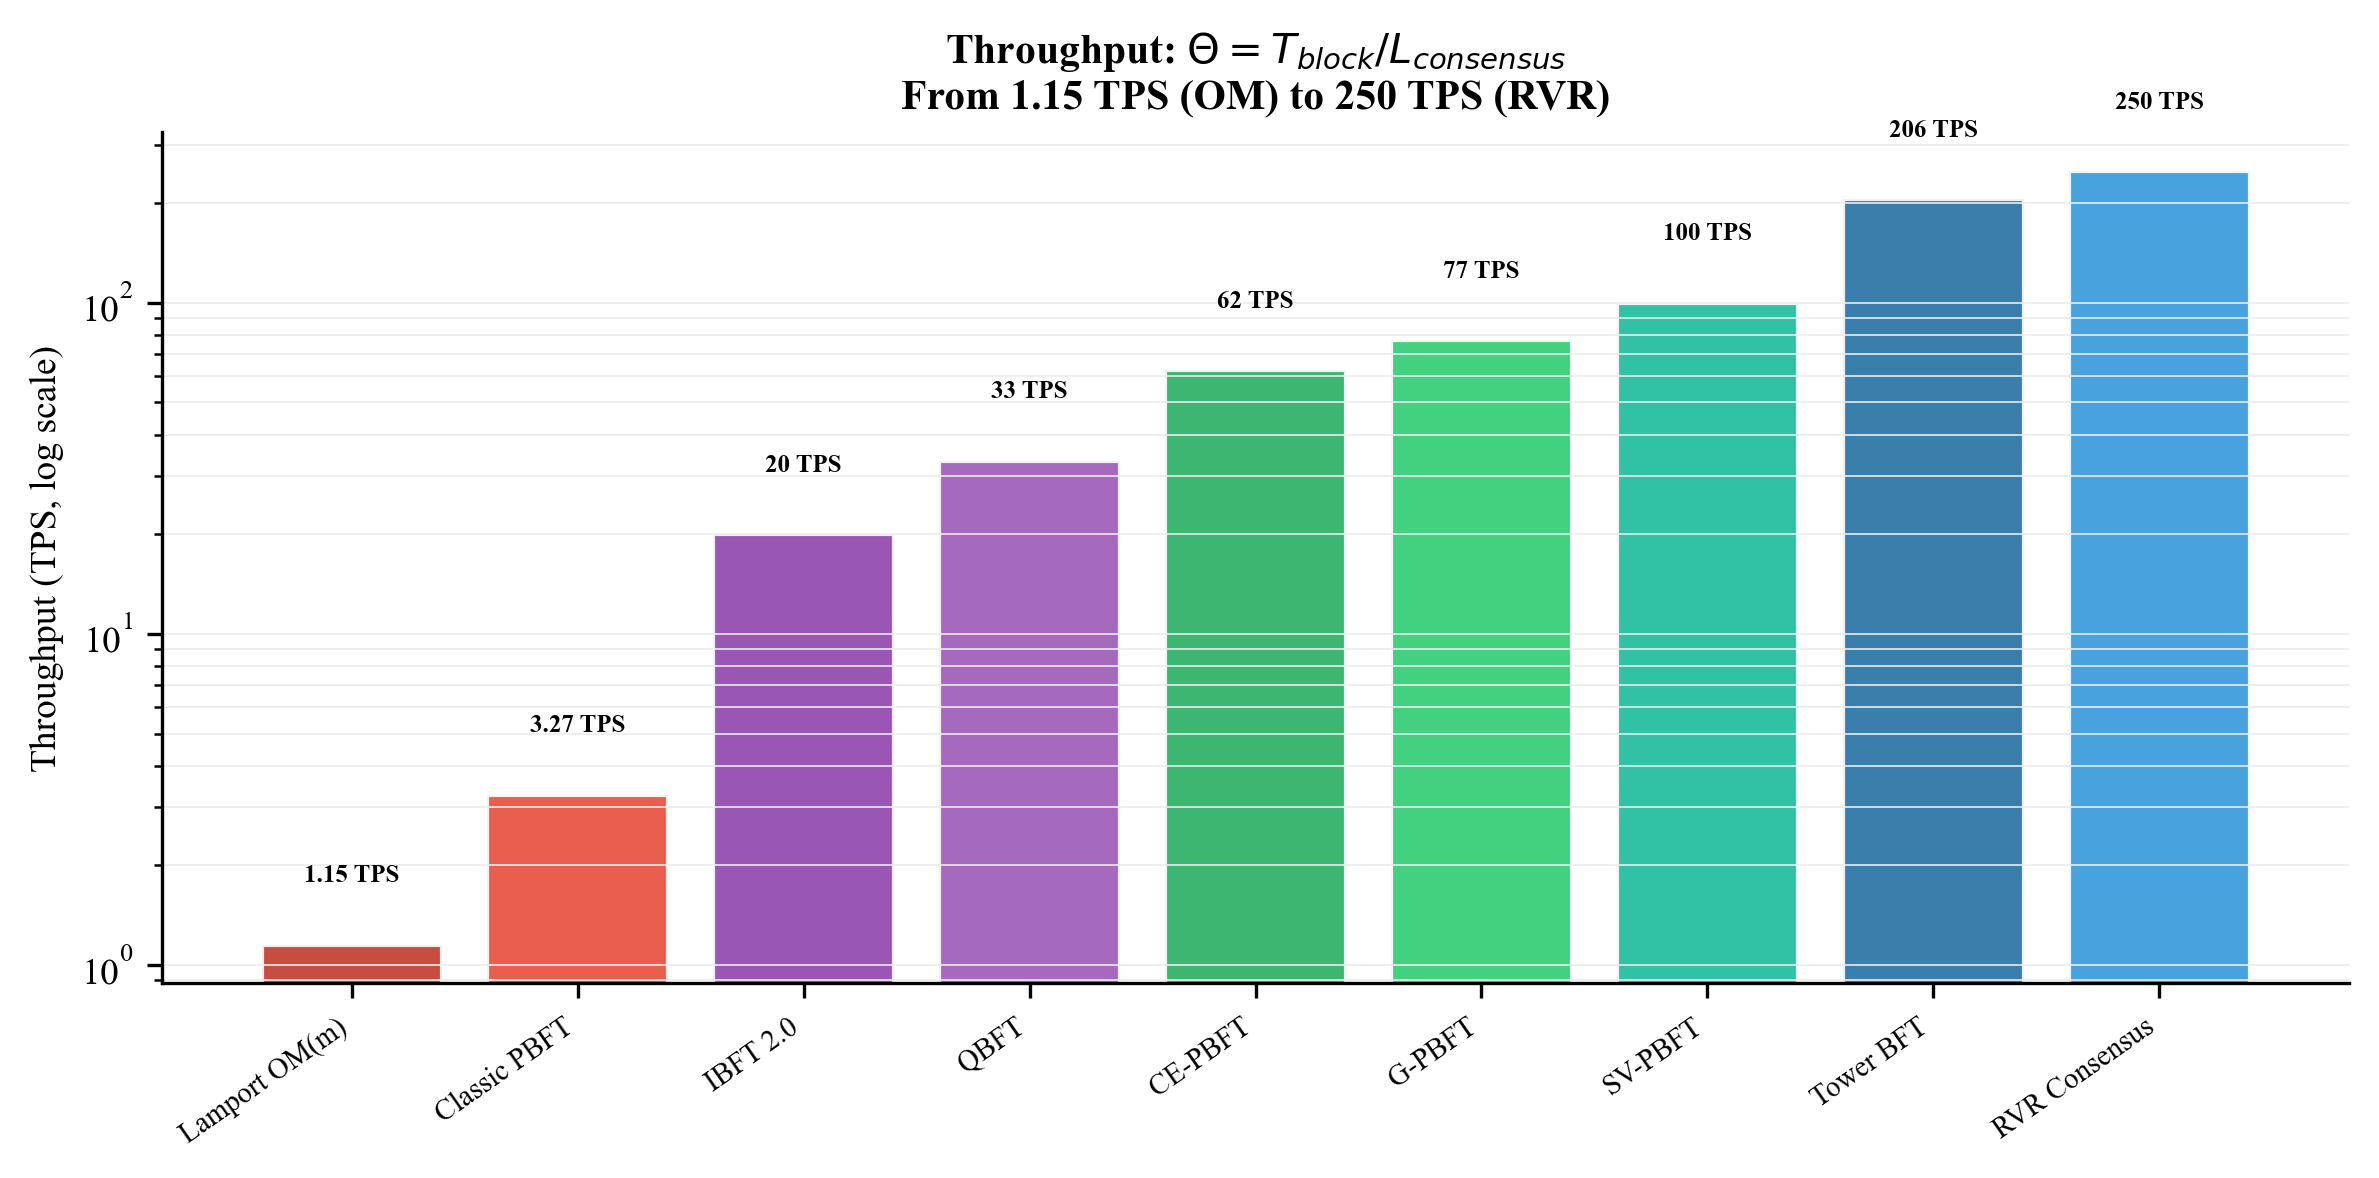
\includegraphics[width=0.75\textwidth]{figures/comparison_throughput.png}
\end{figure}
\clearpage

\section{Comparison Waterfall}
\textbf{File:} \texttt{comparison\_waterfall.png} \\
\textbf{Concept/Origin:} This plot visualizes \textbf{Comparison Waterfall Metric} as a function of \textbf{Time / Baseline Parameter}. \\
\textbf{Equations/Framework:} 
Empirical baseline calculation from simulation data.
\vspace{0.5cm}
\begin{figure}[H]
    \centering
    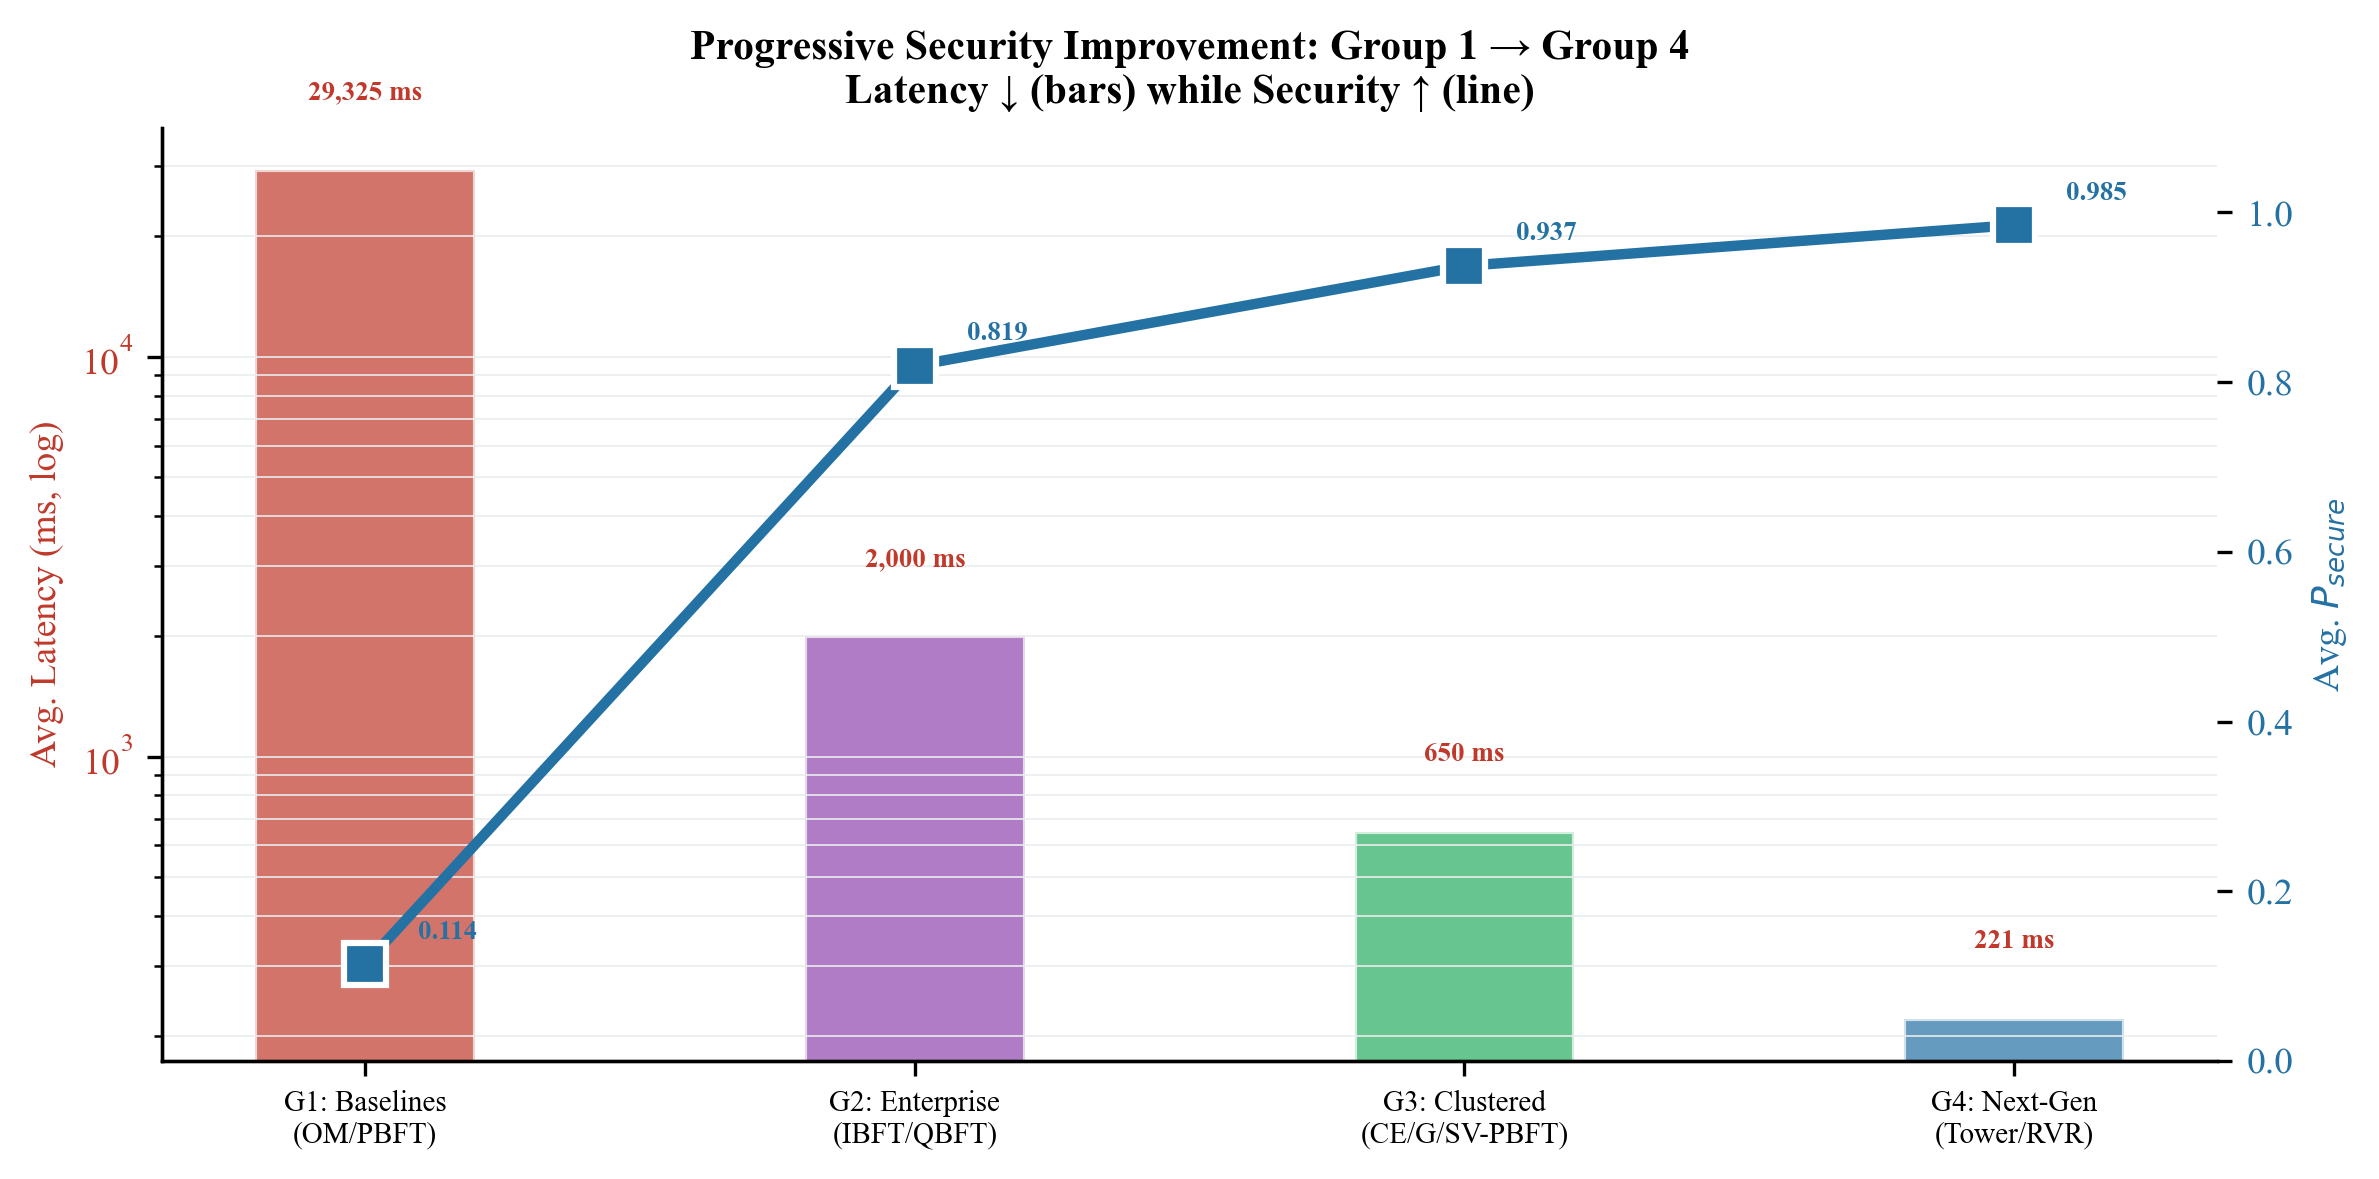
\includegraphics[width=0.75\textwidth]{figures/comparison_waterfall.png}
\end{figure}
\clearpage

\section{Energy Accuracy}
\textbf{File:} \texttt{fig10\_energy\_accuracy.png} \\
\textbf{Concept/Origin:} This plot visualizes \textbf{Energy Accuracy Metric} as a function of \textbf{Time / Baseline Parameter}. \\
\textbf{Equations/Framework:} 
 E_{total} = E_{tx} + E_{rx} + E_{crypto} 
\vspace{0.5cm}
\begin{figure}[H]
    \centering
    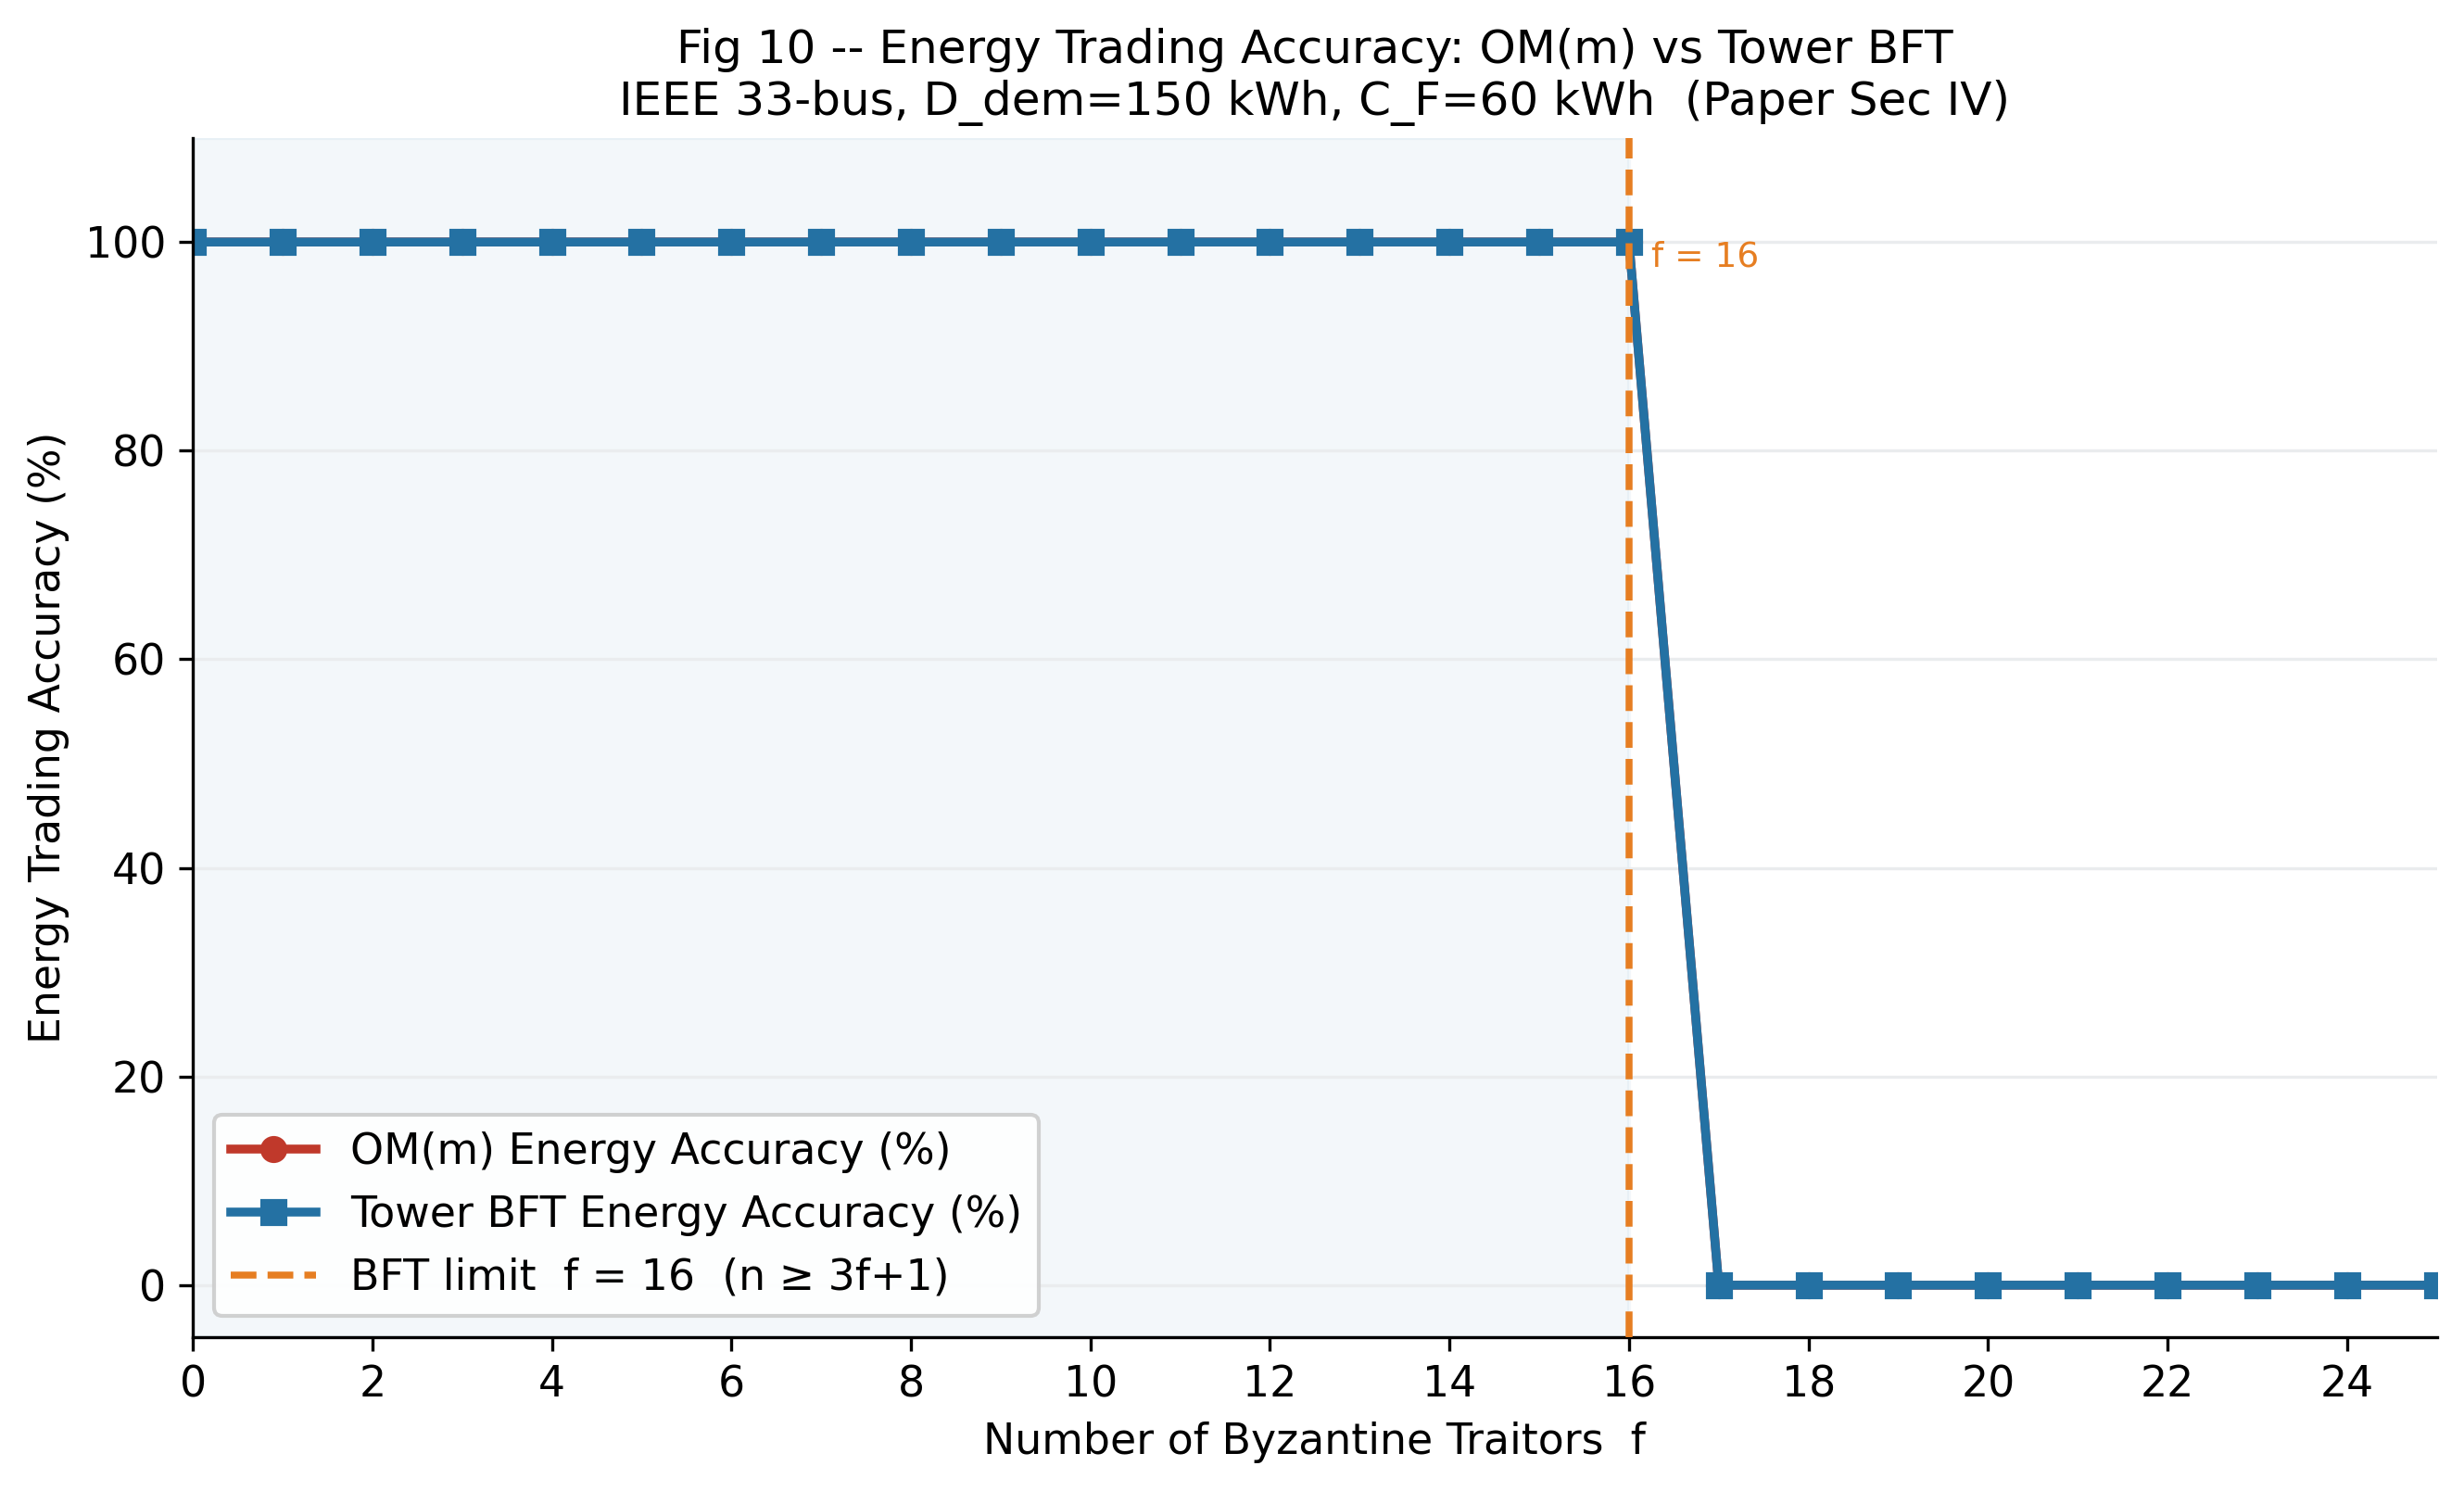
\includegraphics[width=0.75\textwidth]{figures/fig10_energy_accuracy.png}
\end{figure}
\clearpage

\section{Vulnerability Window}
\textbf{File:} \texttt{fig11\_vulnerability\_window.png} \\
\textbf{Concept/Origin:} This plot visualizes \textbf{Vulnerability Window Metric} as a function of \textbf{Time / Baseline Parameter}. \\
\textbf{Equations/Framework:} 
 P_{Byz} = \sum_{i=f+1}^{n} \binom{n}{i} p_c^i (1-p_c)^{n-i} 
 P_{temporal} = 1 - e^{-\lambda L P_{TA}} 
\vspace{0.5cm}
\begin{figure}[H]
    \centering
    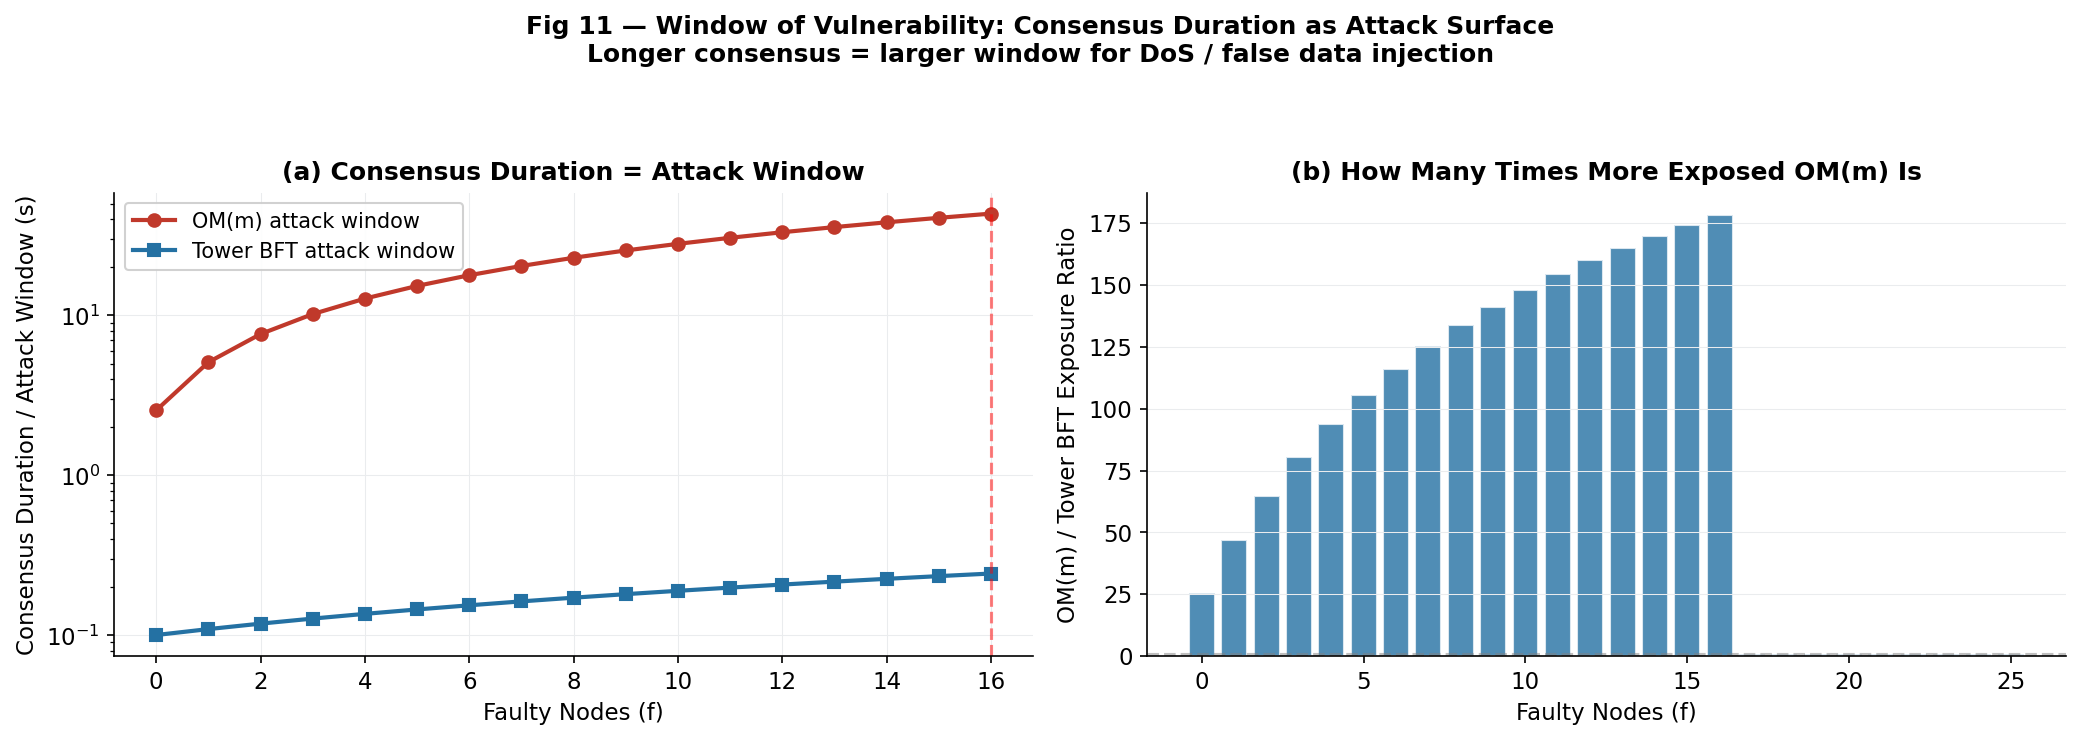
\includegraphics[width=0.75\textwidth]{figures/fig11_vulnerability_window.png}
\end{figure}
\clearpage

\section{Latency Sensitivity}
\textbf{File:} \texttt{fig12\_latency\_sensitivity.png} \\
\textbf{Concept/Origin:} This plot visualizes \textbf{Latency Sensitivity Metric} as a function of \textbf{Time / Baseline Parameter}. \\
\textbf{Equations/Framework:} 
 L_{total} = L_{net} + L_{consensus} 
\vspace{0.5cm}
\begin{figure}[H]
    \centering
    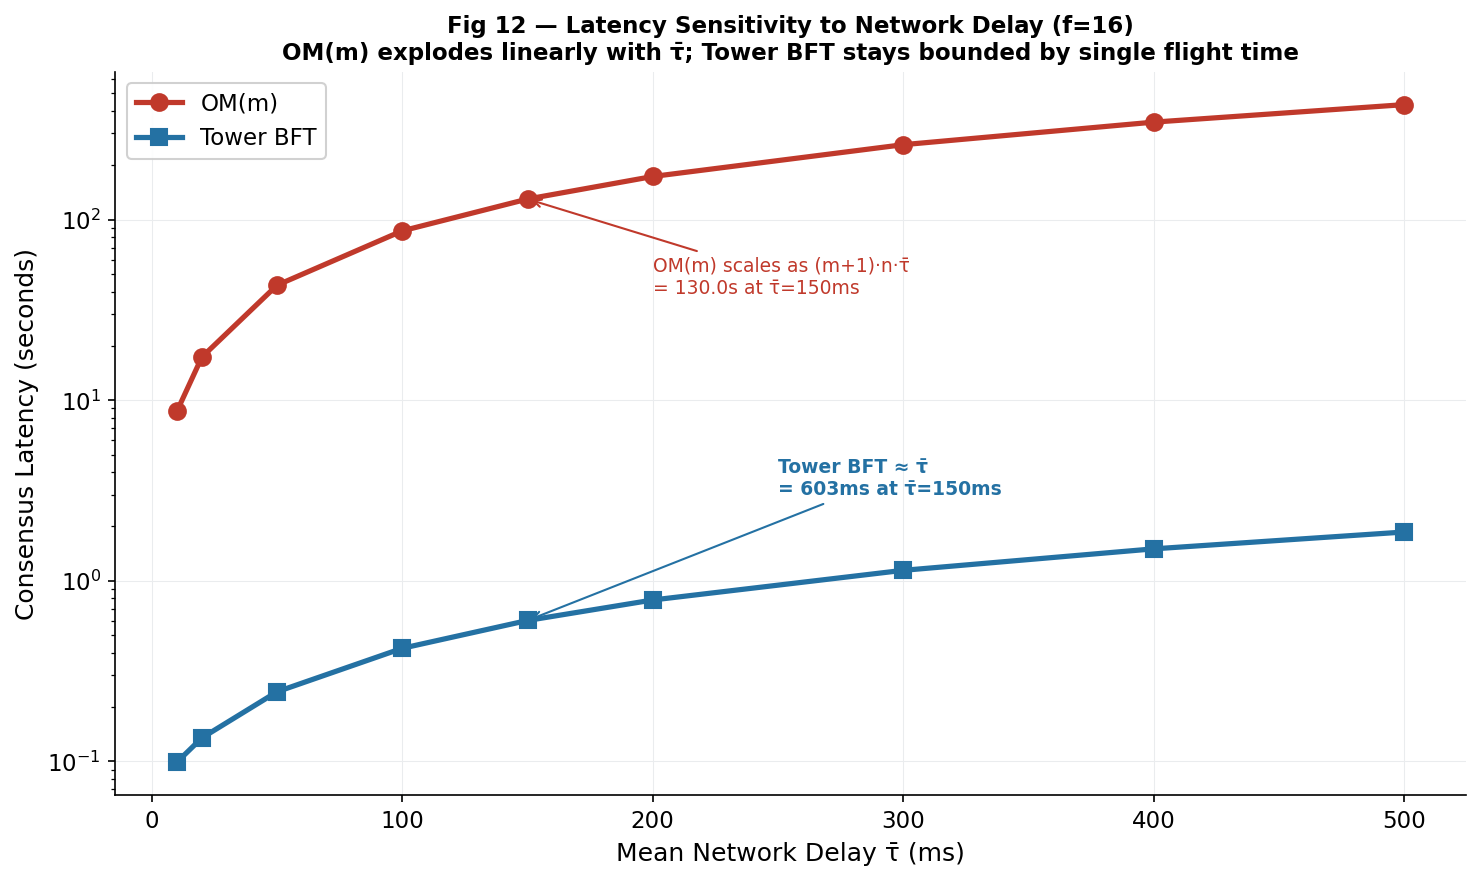
\includegraphics[width=0.75\textwidth]{figures/fig12_latency_sensitivity.png}
\end{figure}
\clearpage

\section{Packet Loss Resilience}
\textbf{File:} \texttt{fig13\_packet\_loss\_resilience.png} \\
\textbf{Concept/Origin:} This plot visualizes \textbf{Packet Loss Resilience Metric} as a function of \textbf{Time / Baseline Parameter}. \\
\textbf{Equations/Framework:} 
Empirical baseline calculation from simulation data.
\vspace{0.5cm}
\begin{figure}[H]
    \centering
    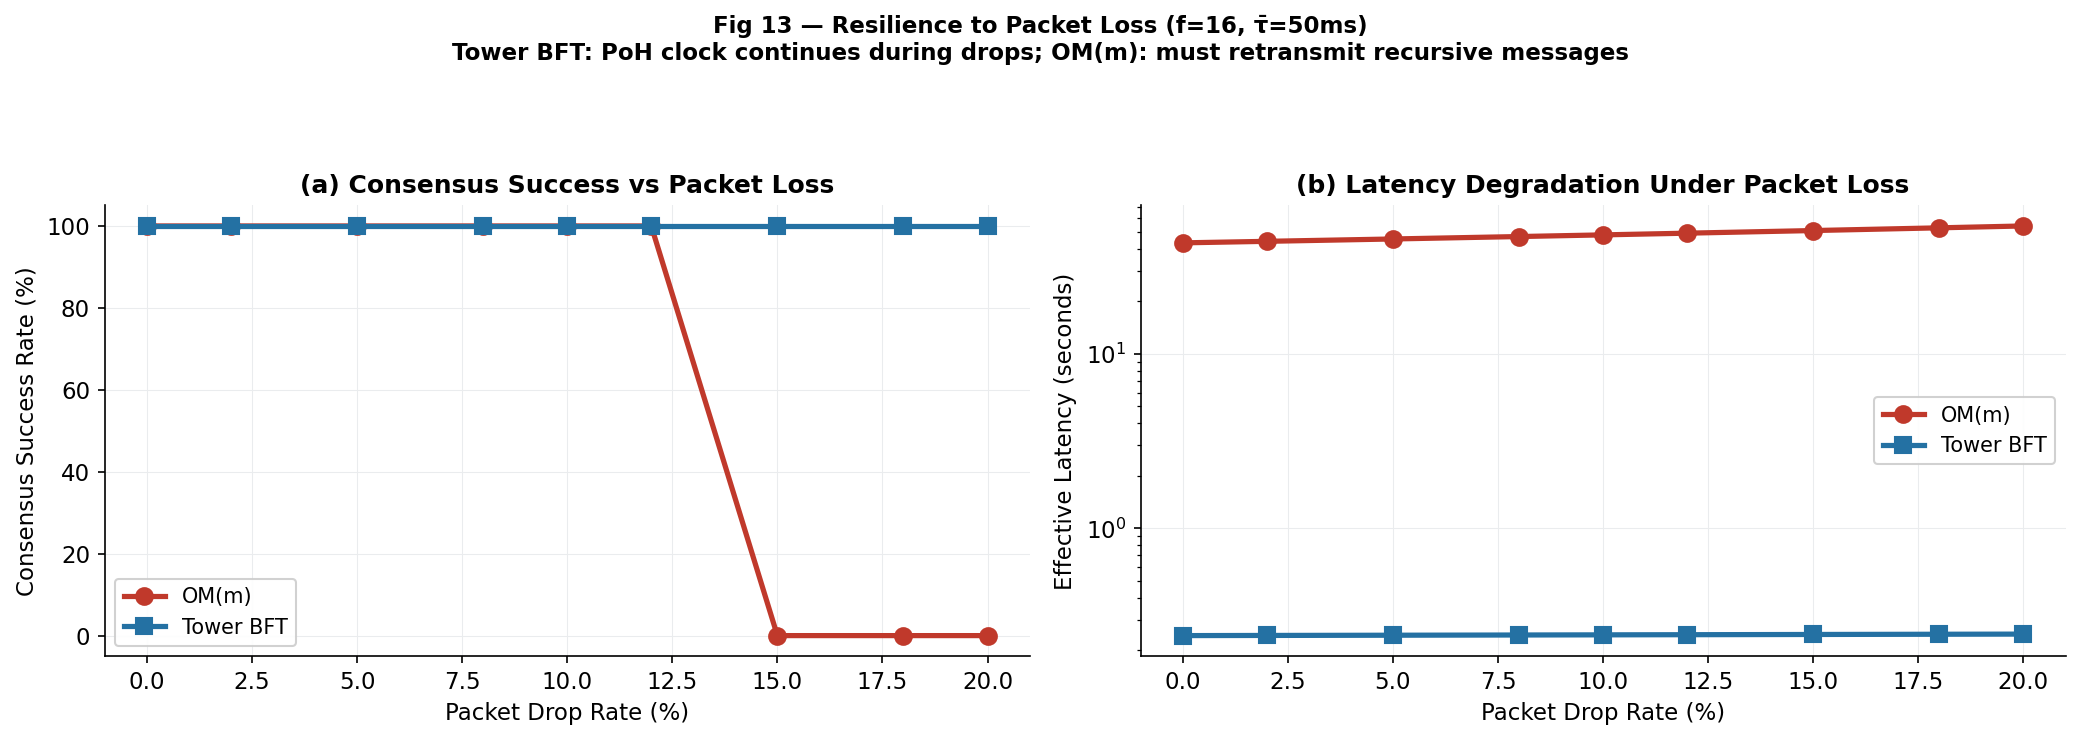
\includegraphics[width=0.75\textwidth]{figures/fig13_packet_loss_resilience.png}
\end{figure}
\clearpage

\section{Pta No Blockchain}
\textbf{File:} \texttt{fig15\_pta\_no\_blockchain.png} \\
\textbf{Concept/Origin:} This plot visualizes \textbf{Pta No Blockchain Metric} as a function of \textbf{Time / Baseline Parameter}. \\
\textbf{Equations/Framework:} 
Empirical baseline calculation from simulation data.
\vspace{0.5cm}
\begin{figure}[H]
    \centering
    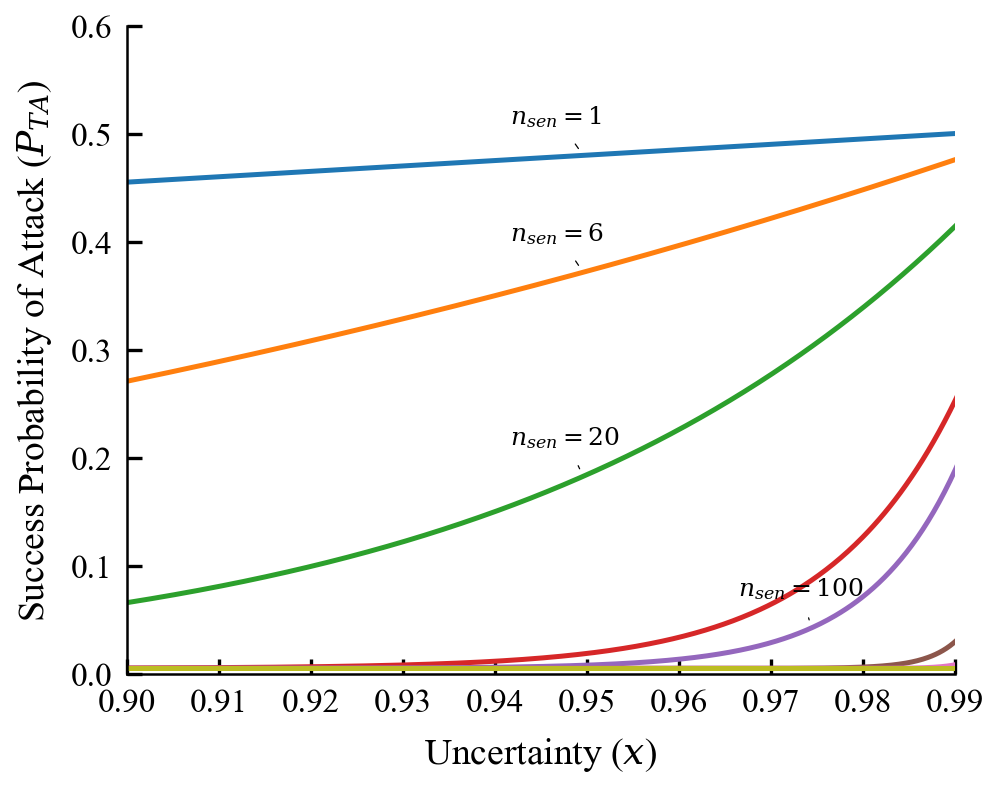
\includegraphics[width=0.75\textwidth]{figures/fig15_pta_no_blockchain.png}
\end{figure}
\clearpage

\section{Ptab With Blockchain}
\textbf{File:} \texttt{fig16\_ptab\_with\_blockchain.png} \\
\textbf{Concept/Origin:} This plot visualizes \textbf{Ptab With Blockchain Metric} as a function of \textbf{Time / Baseline Parameter}. \\
\textbf{Equations/Framework:} 
Empirical baseline calculation from simulation data.
\vspace{0.5cm}
\begin{figure}[H]
    \centering
    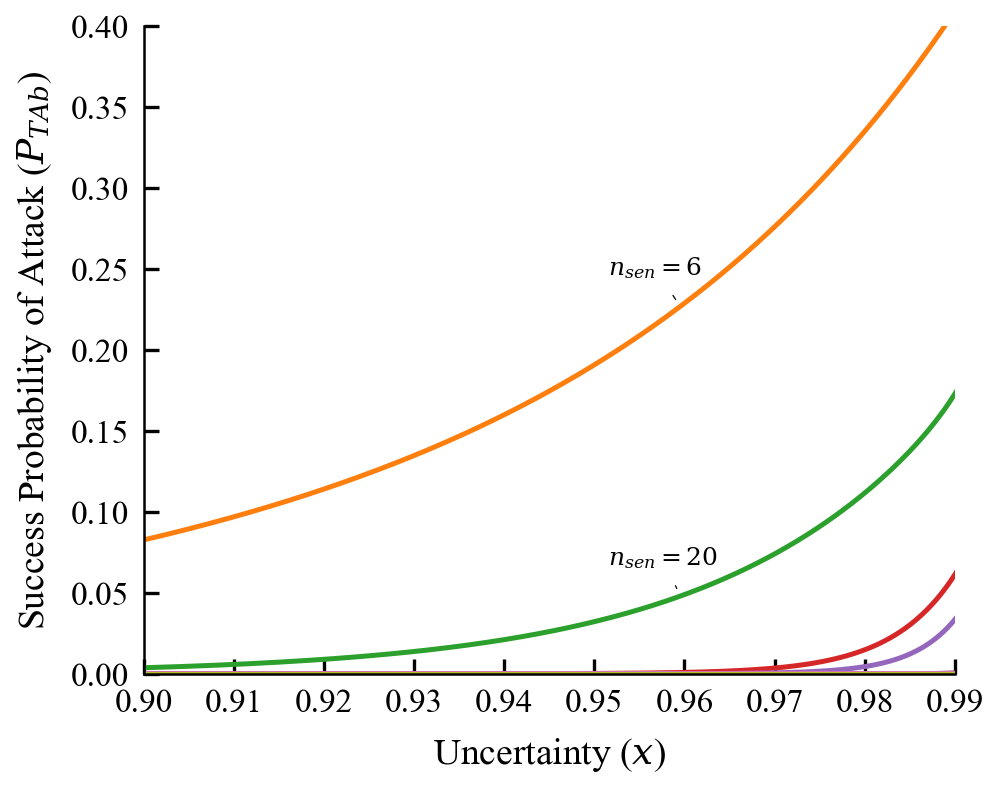
\includegraphics[width=0.75\textwidth]{figures/fig16_ptab_with_blockchain.png}
\end{figure}
\clearpage

\section{Bft Vs Tbft Comparison}
\textbf{File:} \texttt{fig17\_bft\_vs\_tbft\_comparison.png} \\
\textbf{Concept/Origin:} This plot visualizes \textbf{Bft} as a function of \textbf{Tbft Comparison}. \\
\textbf{Equations/Framework:} 
Empirical baseline calculation from simulation data.
\vspace{0.5cm}
\begin{figure}[H]
    \centering
    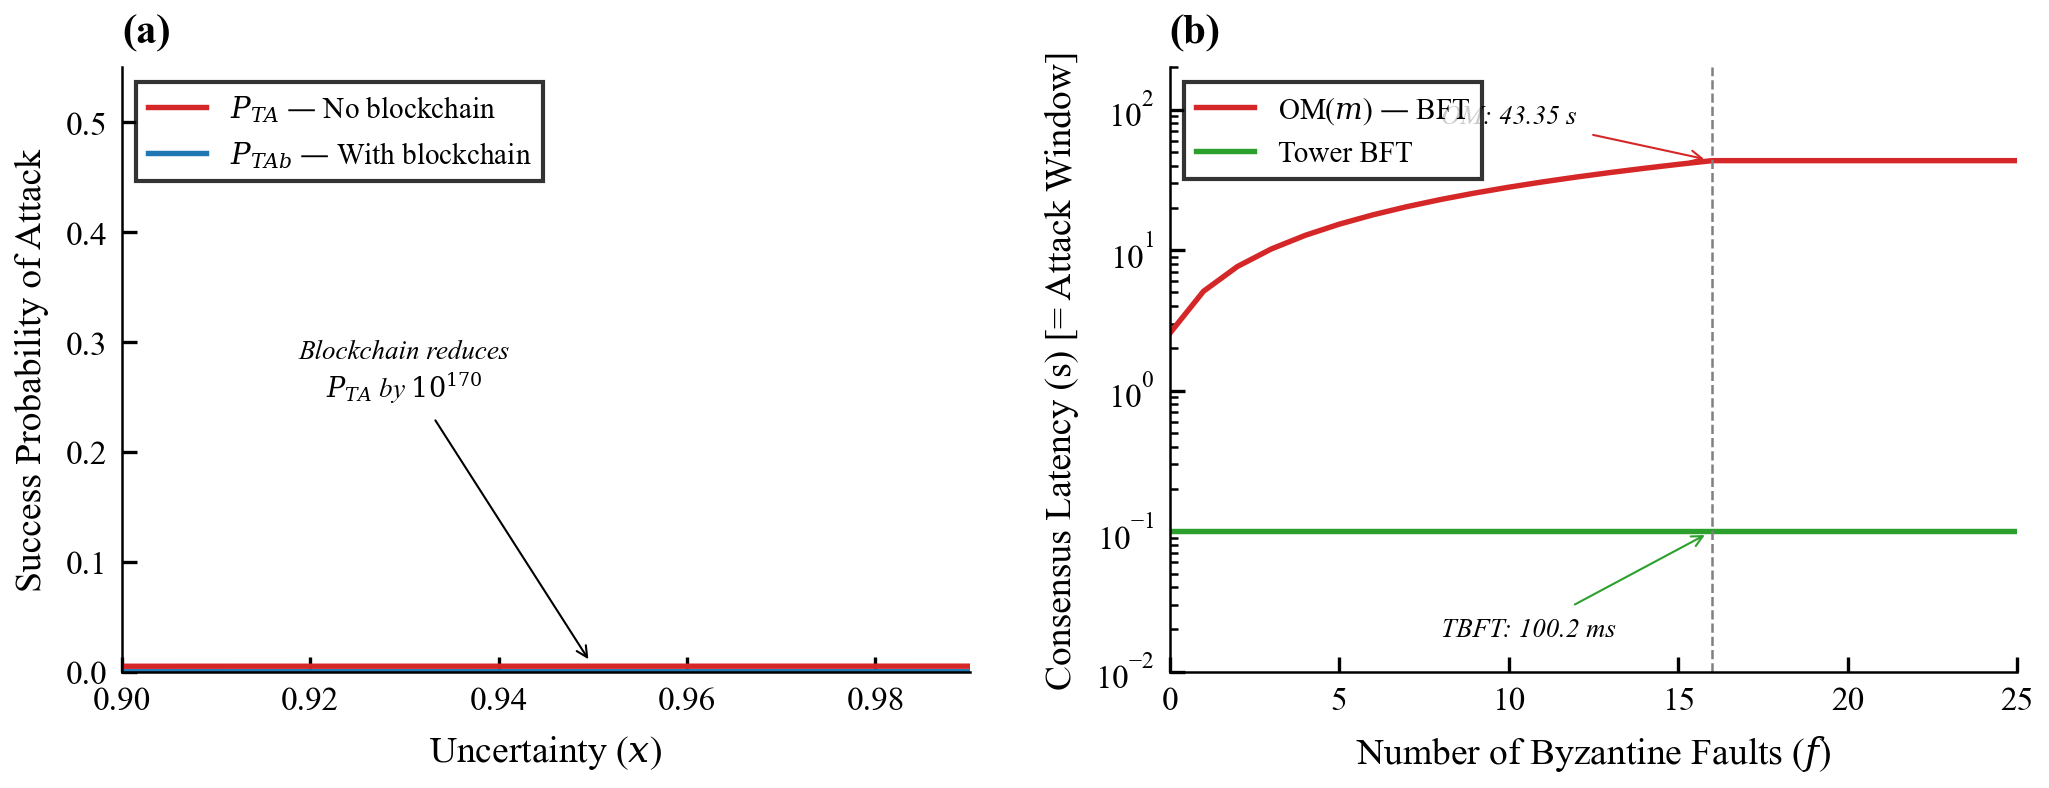
\includegraphics[width=0.75\textwidth]{figures/fig17_bft_vs_tbft_comparison.png}
\end{figure}
\clearpage

\section{Without Vs With Blockchain}
\textbf{File:} \texttt{fig18\_without\_vs\_with\_blockchain.png} \\
\textbf{Concept/Origin:} This plot visualizes \textbf{Without} as a function of \textbf{With Blockchain}. \\
\textbf{Equations/Framework:} 
Empirical baseline calculation from simulation data.
\vspace{0.5cm}
\begin{figure}[H]
    \centering
    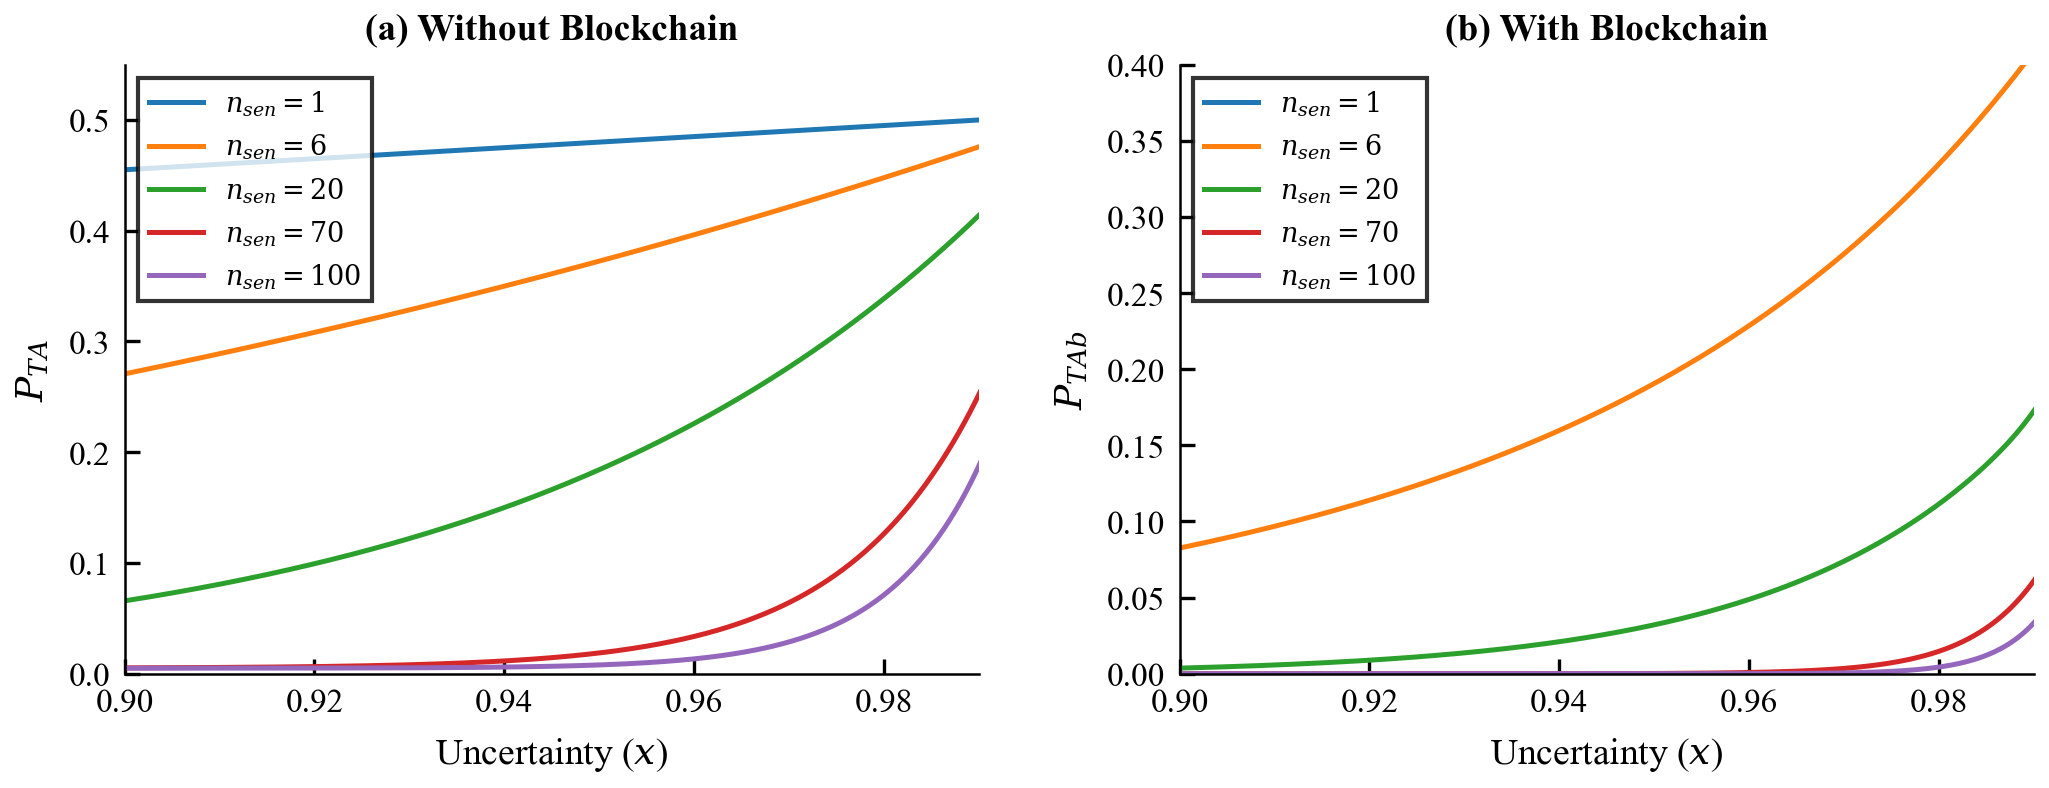
\includegraphics[width=0.75\textwidth]{figures/fig18_without_vs_with_blockchain.png}
\end{figure}
\clearpage

\section{Exposure Bft Vs Tbft}
\textbf{File:} \texttt{fig19\_exposure\_bft\_vs\_tbft.png} \\
\textbf{Concept/Origin:} This plot visualizes \textbf{Exposure Bft} as a function of \textbf{Tbft}. \\
\textbf{Equations/Framework:} 
Empirical baseline calculation from simulation data.
\vspace{0.5cm}
\begin{figure}[H]
    \centering
    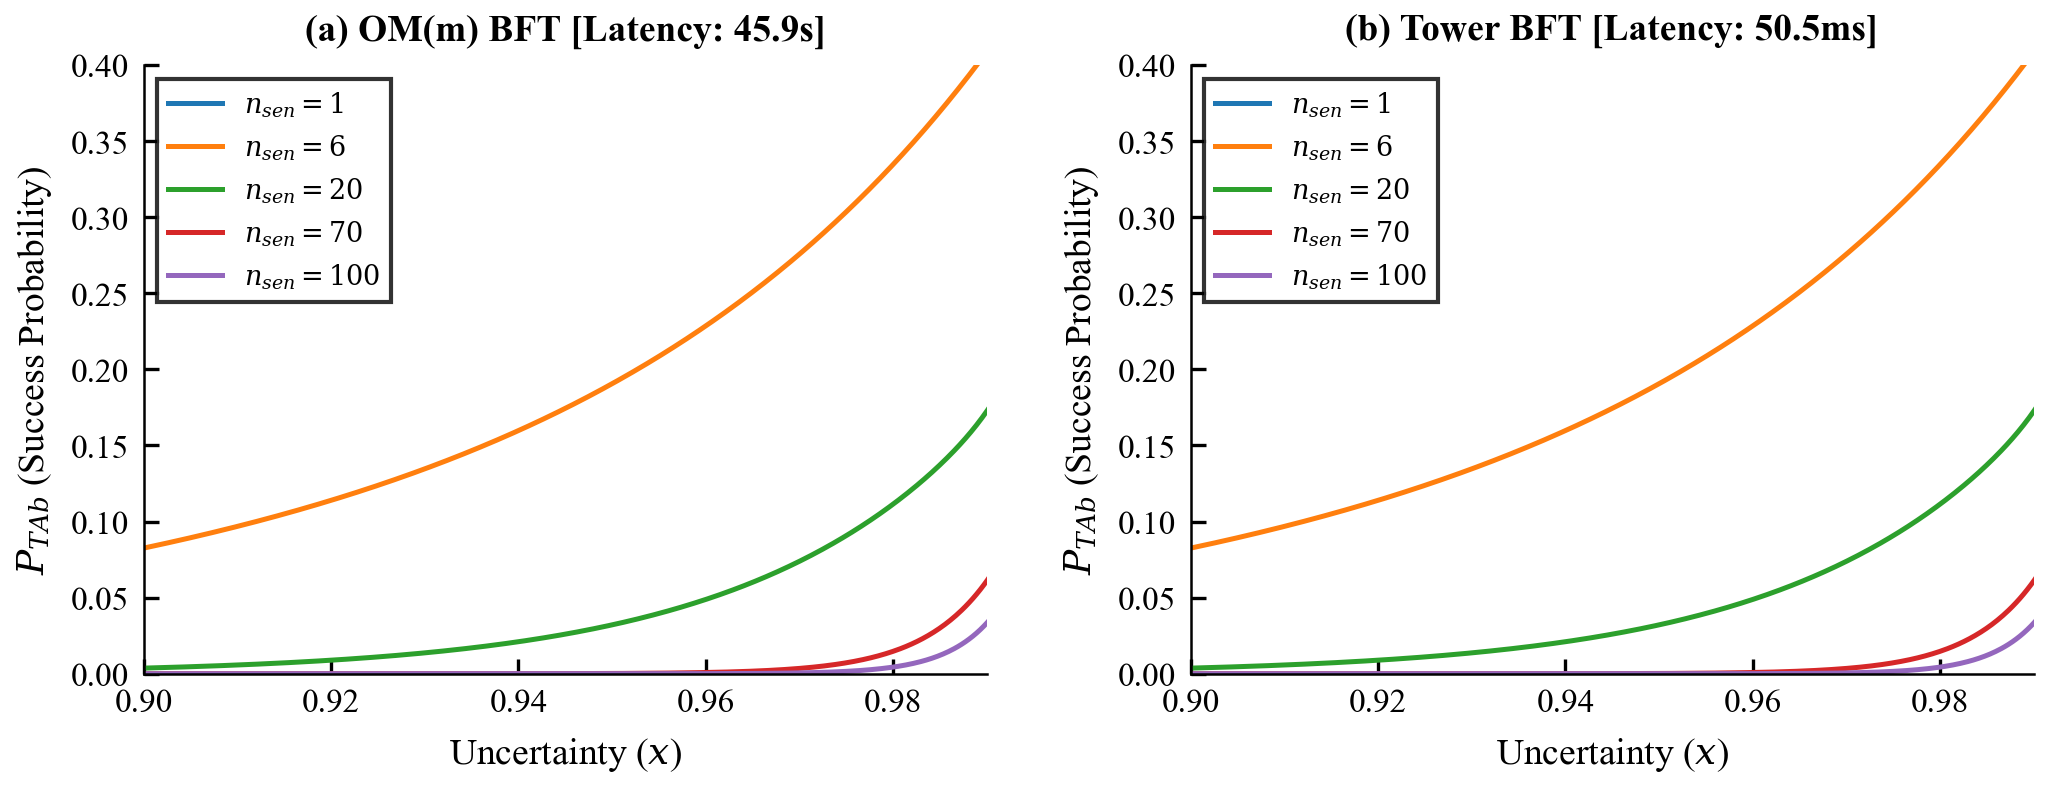
\includegraphics[width=0.75\textwidth]{figures/fig19_exposure_bft_vs_tbft.png}
\end{figure}
\clearpage

\section{Consensus Success Rate}
\textbf{File:} \texttt{fig1\_consensus\_success\_rate.png} \\
\textbf{Concept/Origin:} This plot visualizes \textbf{Consensus Success Rate Metric} as a function of \textbf{Time / Baseline Parameter}. \\
\textbf{Equations/Framework:} 
Empirical baseline calculation from simulation data.
\vspace{0.5cm}
\begin{figure}[H]
    \centering
    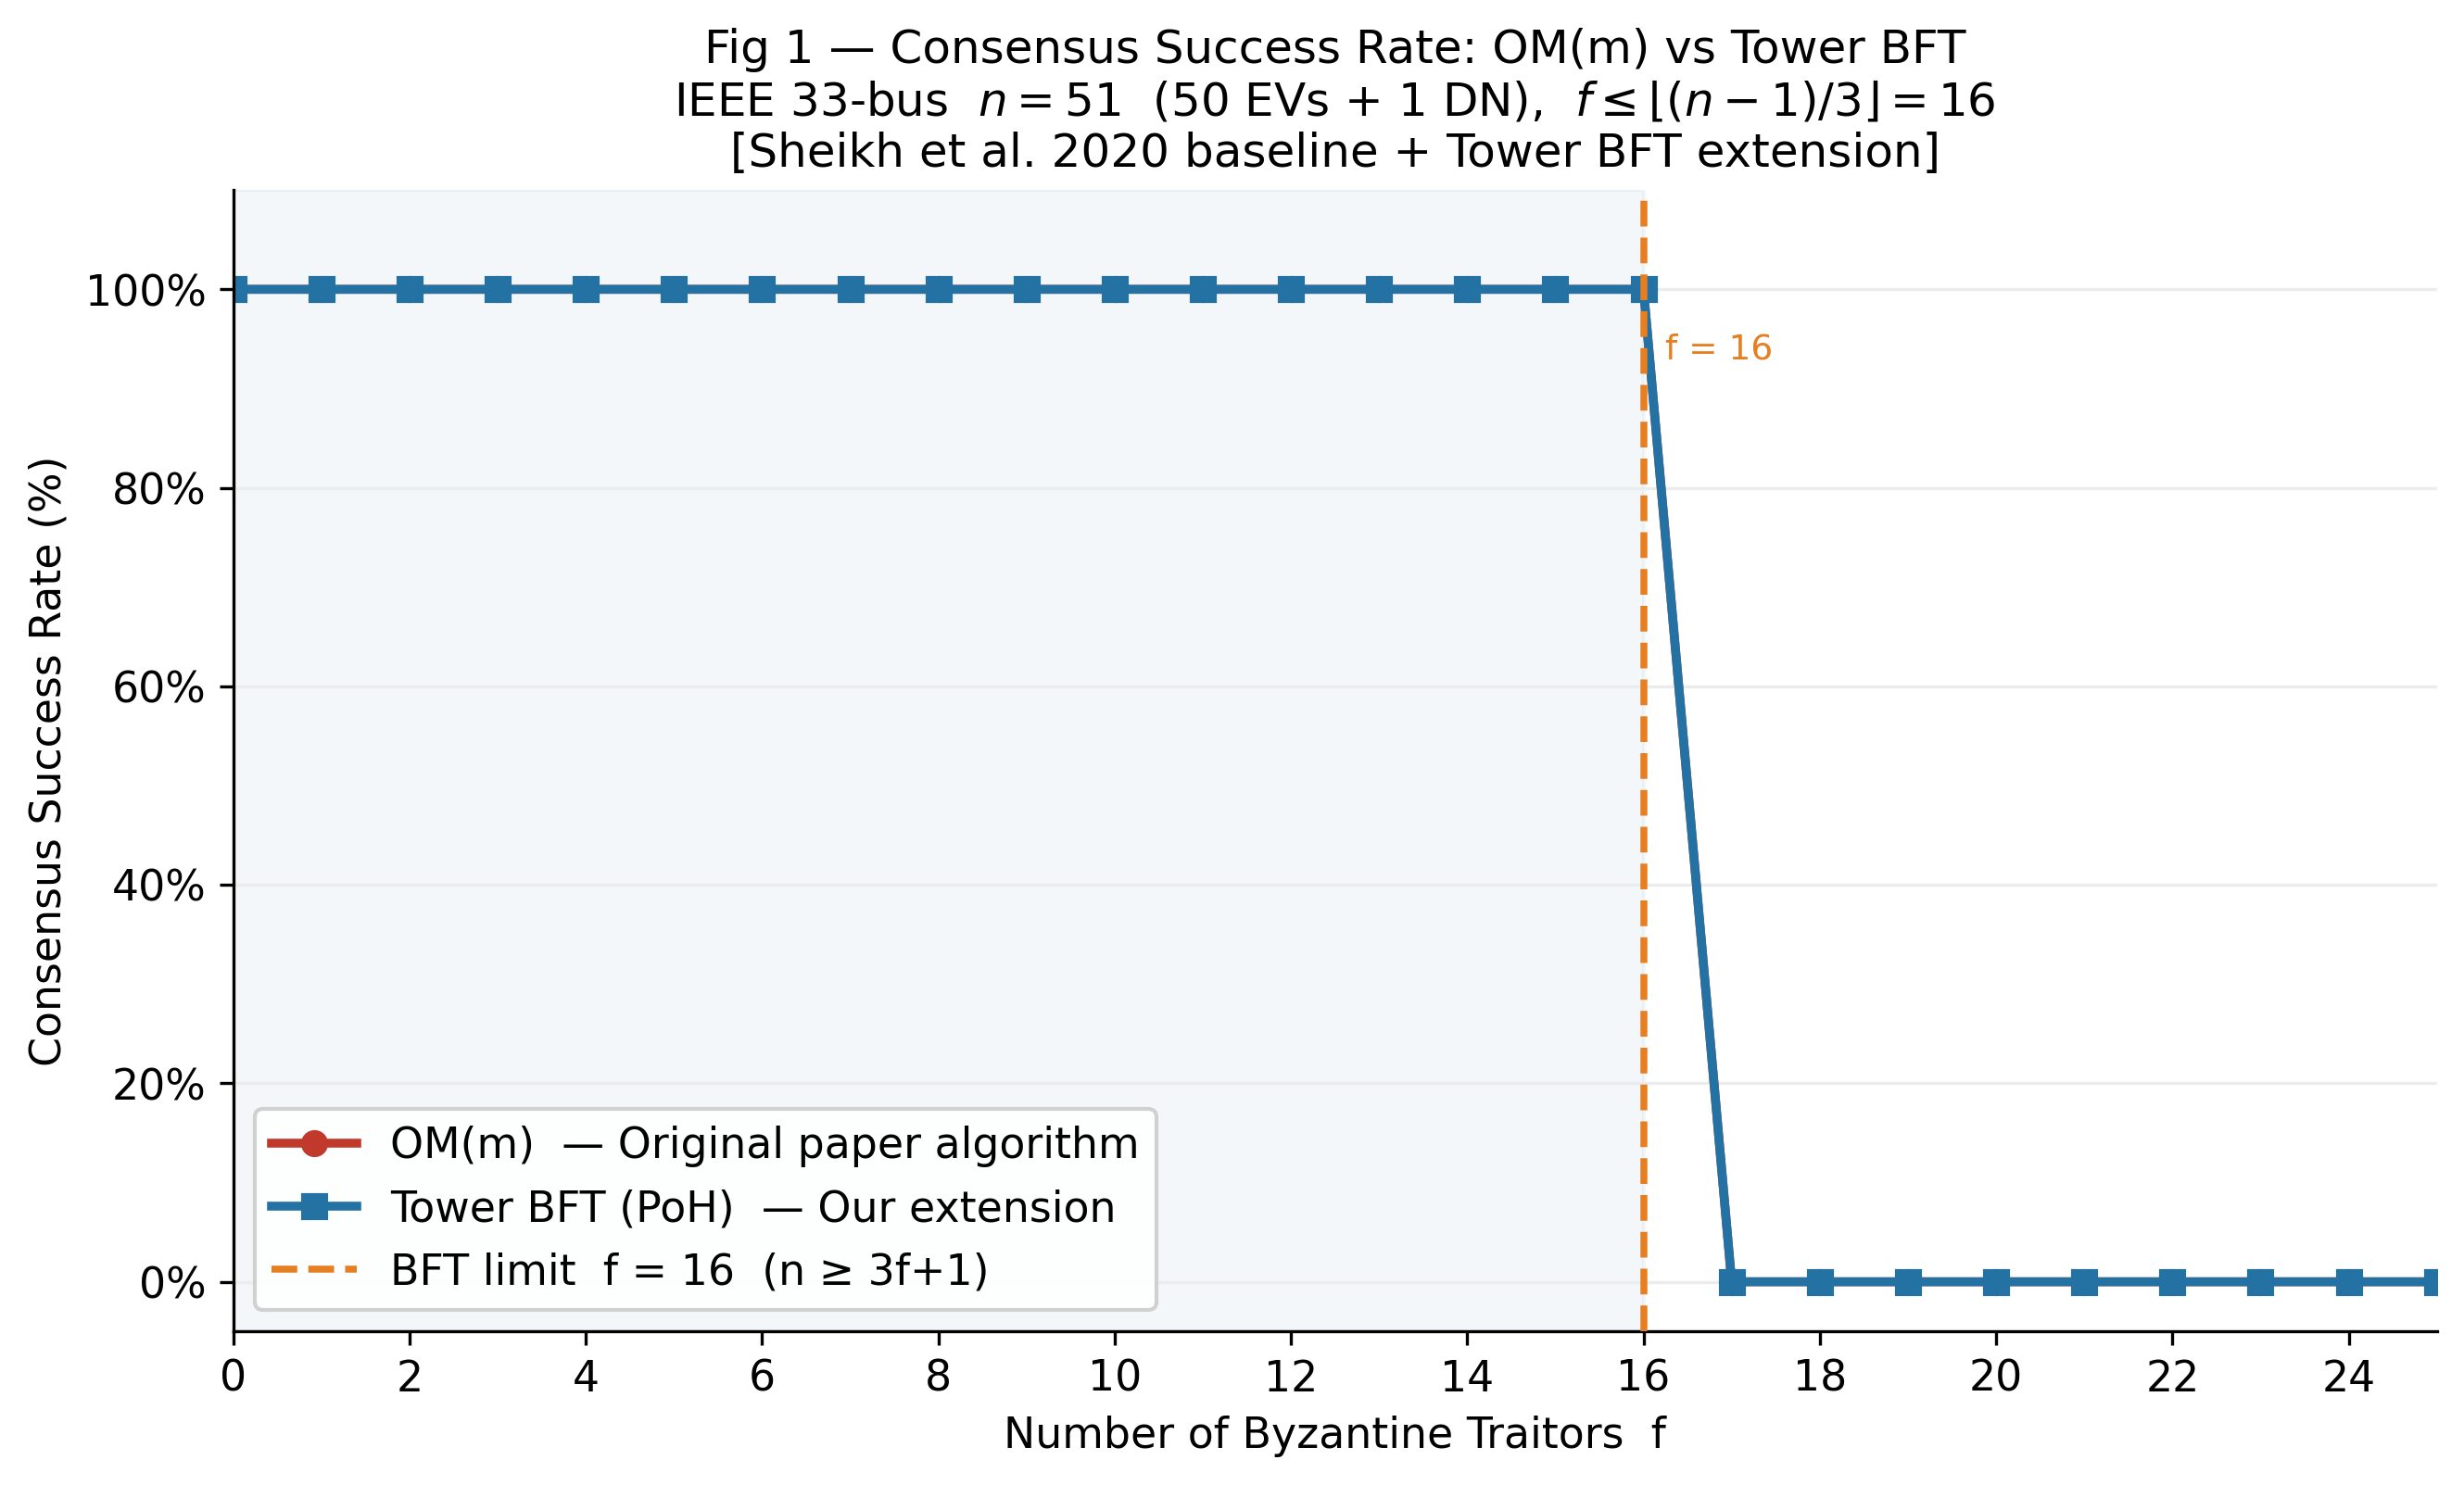
\includegraphics[width=0.75\textwidth]{figures/fig1_consensus_success_rate.png}
\end{figure}
\clearpage

\section{Latency Adjusted Probability}
\textbf{File:} \texttt{fig20\_latency\_adjusted\_probability.png} \\
\textbf{Concept/Origin:} This plot visualizes \textbf{Latency Adjusted Probability Metric} as a function of \textbf{Time / Baseline Parameter}. \\
\textbf{Equations/Framework:} 
 L_{total} = L_{net} + L_{consensus} 
\vspace{0.5cm}
\begin{figure}[H]
    \centering
    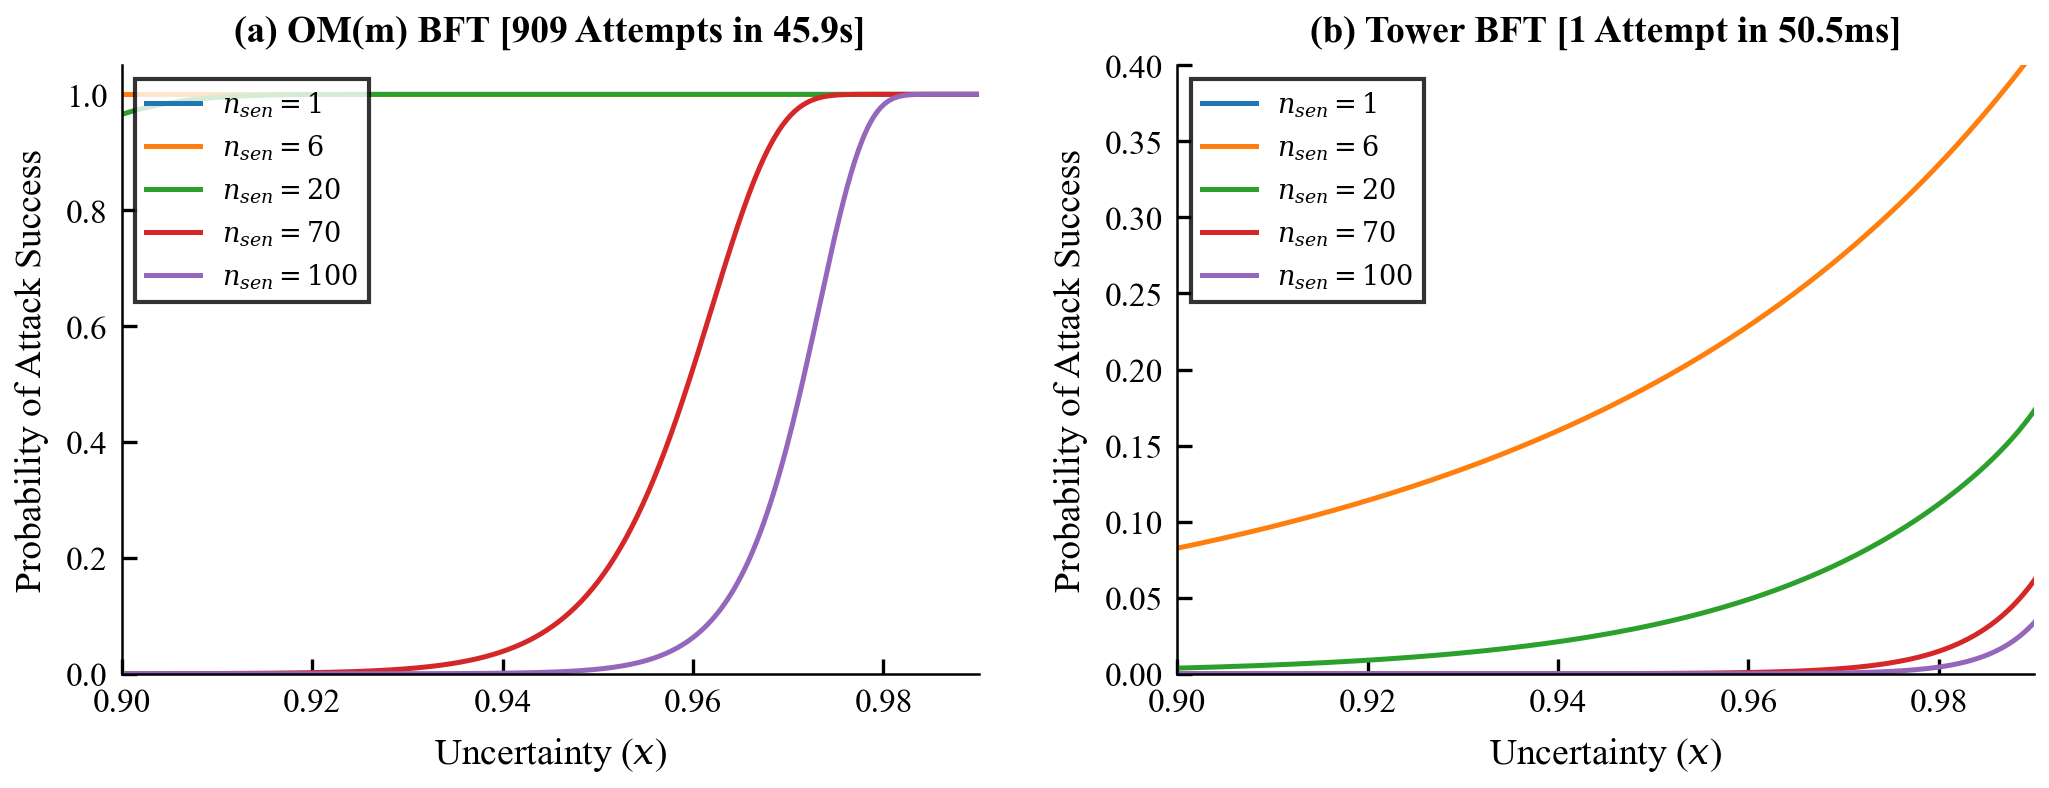
\includegraphics[width=0.75\textwidth]{figures/fig20_latency_adjusted_probability.png}
\end{figure}
\clearpage

\section{Prob Vs Time}
\textbf{File:} \texttt{fig21\_prob\_vs\_time.png} \\
\textbf{Concept/Origin:} This plot visualizes \textbf{Prob} as a function of \textbf{Time}. \\
\textbf{Equations/Framework:} 
 P_{Byz} = \sum_{i=f+1}^{n} \binom{n}{i} p_c^i (1-p_c)^{n-i} 
 P_{temporal} = 1 - e^{-\lambda L P_{TA}} 
\vspace{0.5cm}
\begin{figure}[H]
    \centering
    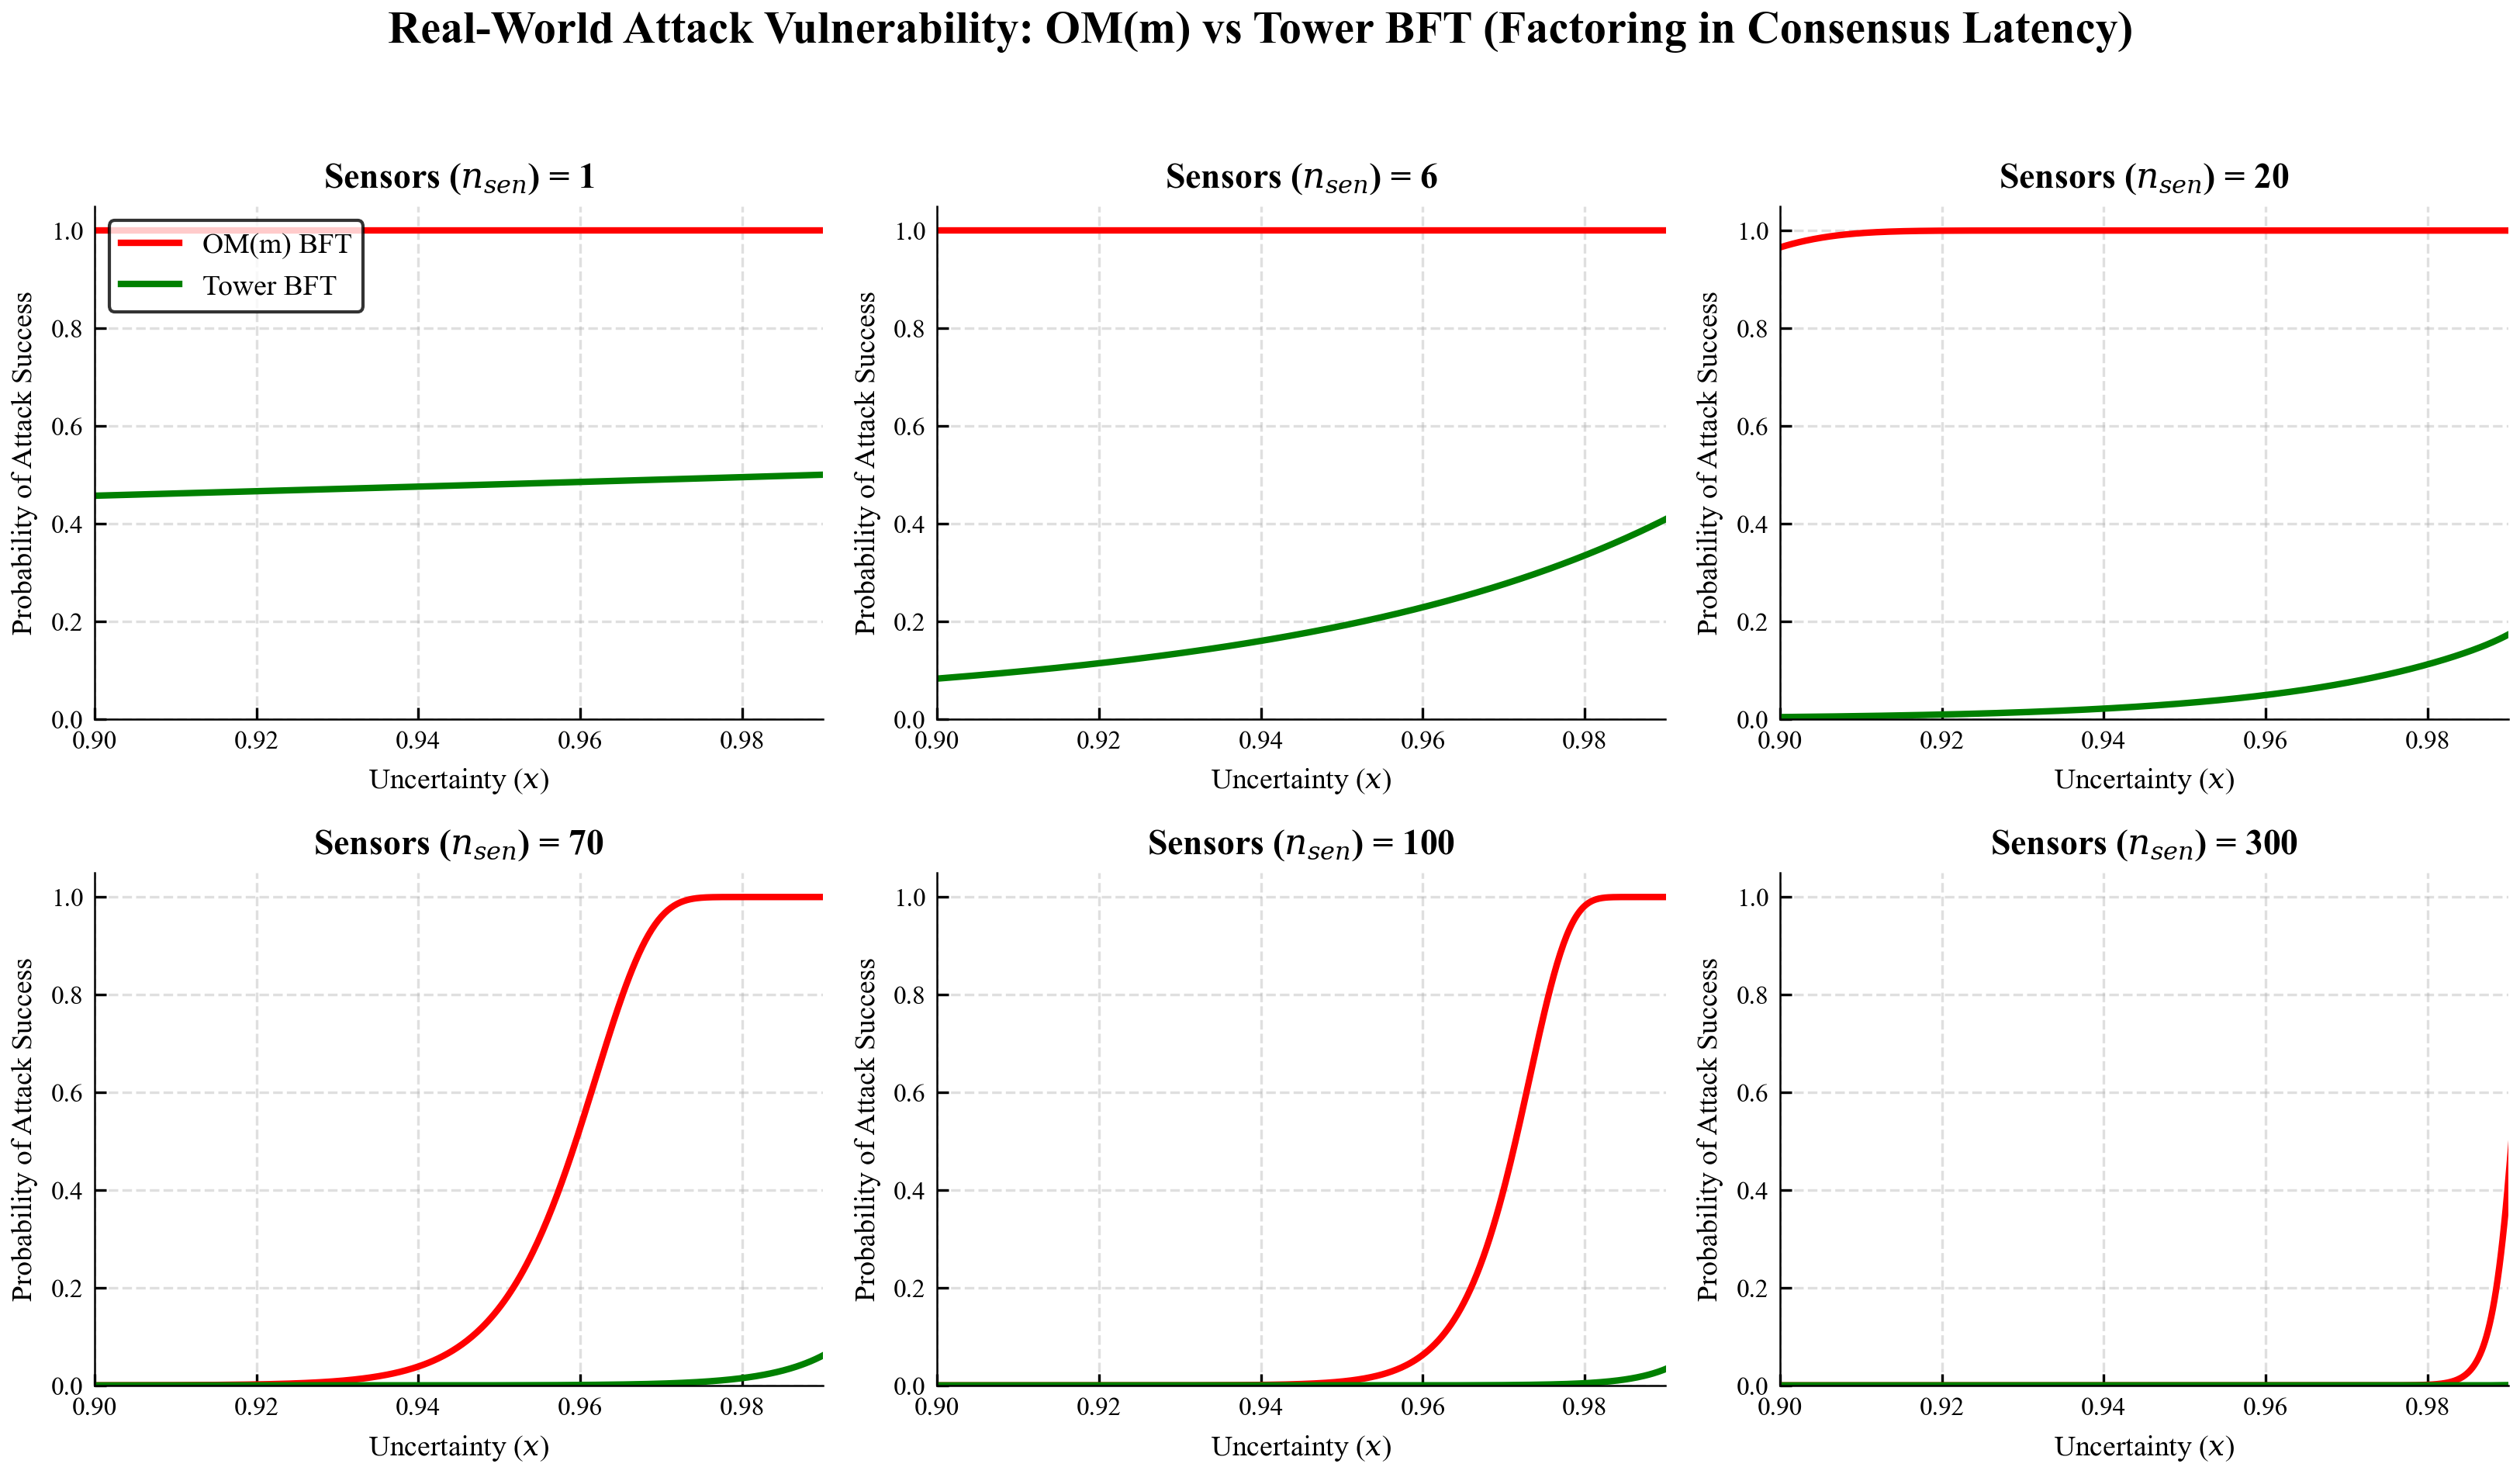
\includegraphics[width=0.75\textwidth]{figures/fig21_prob_vs_time.png}
\end{figure}
\clearpage

\section{Message Complexity}
\textbf{File:} \texttt{fig2\_message\_complexity.png} \\
\textbf{Concept/Origin:} This plot visualizes \textbf{Message Complexity Metric} as a function of \textbf{Time / Baseline Parameter}. \\
\textbf{Equations/Framework:} 
 E_{total} = E_{tx} + E_{rx} + E_{crypto} 
\vspace{0.5cm}
\begin{figure}[H]
    \centering
    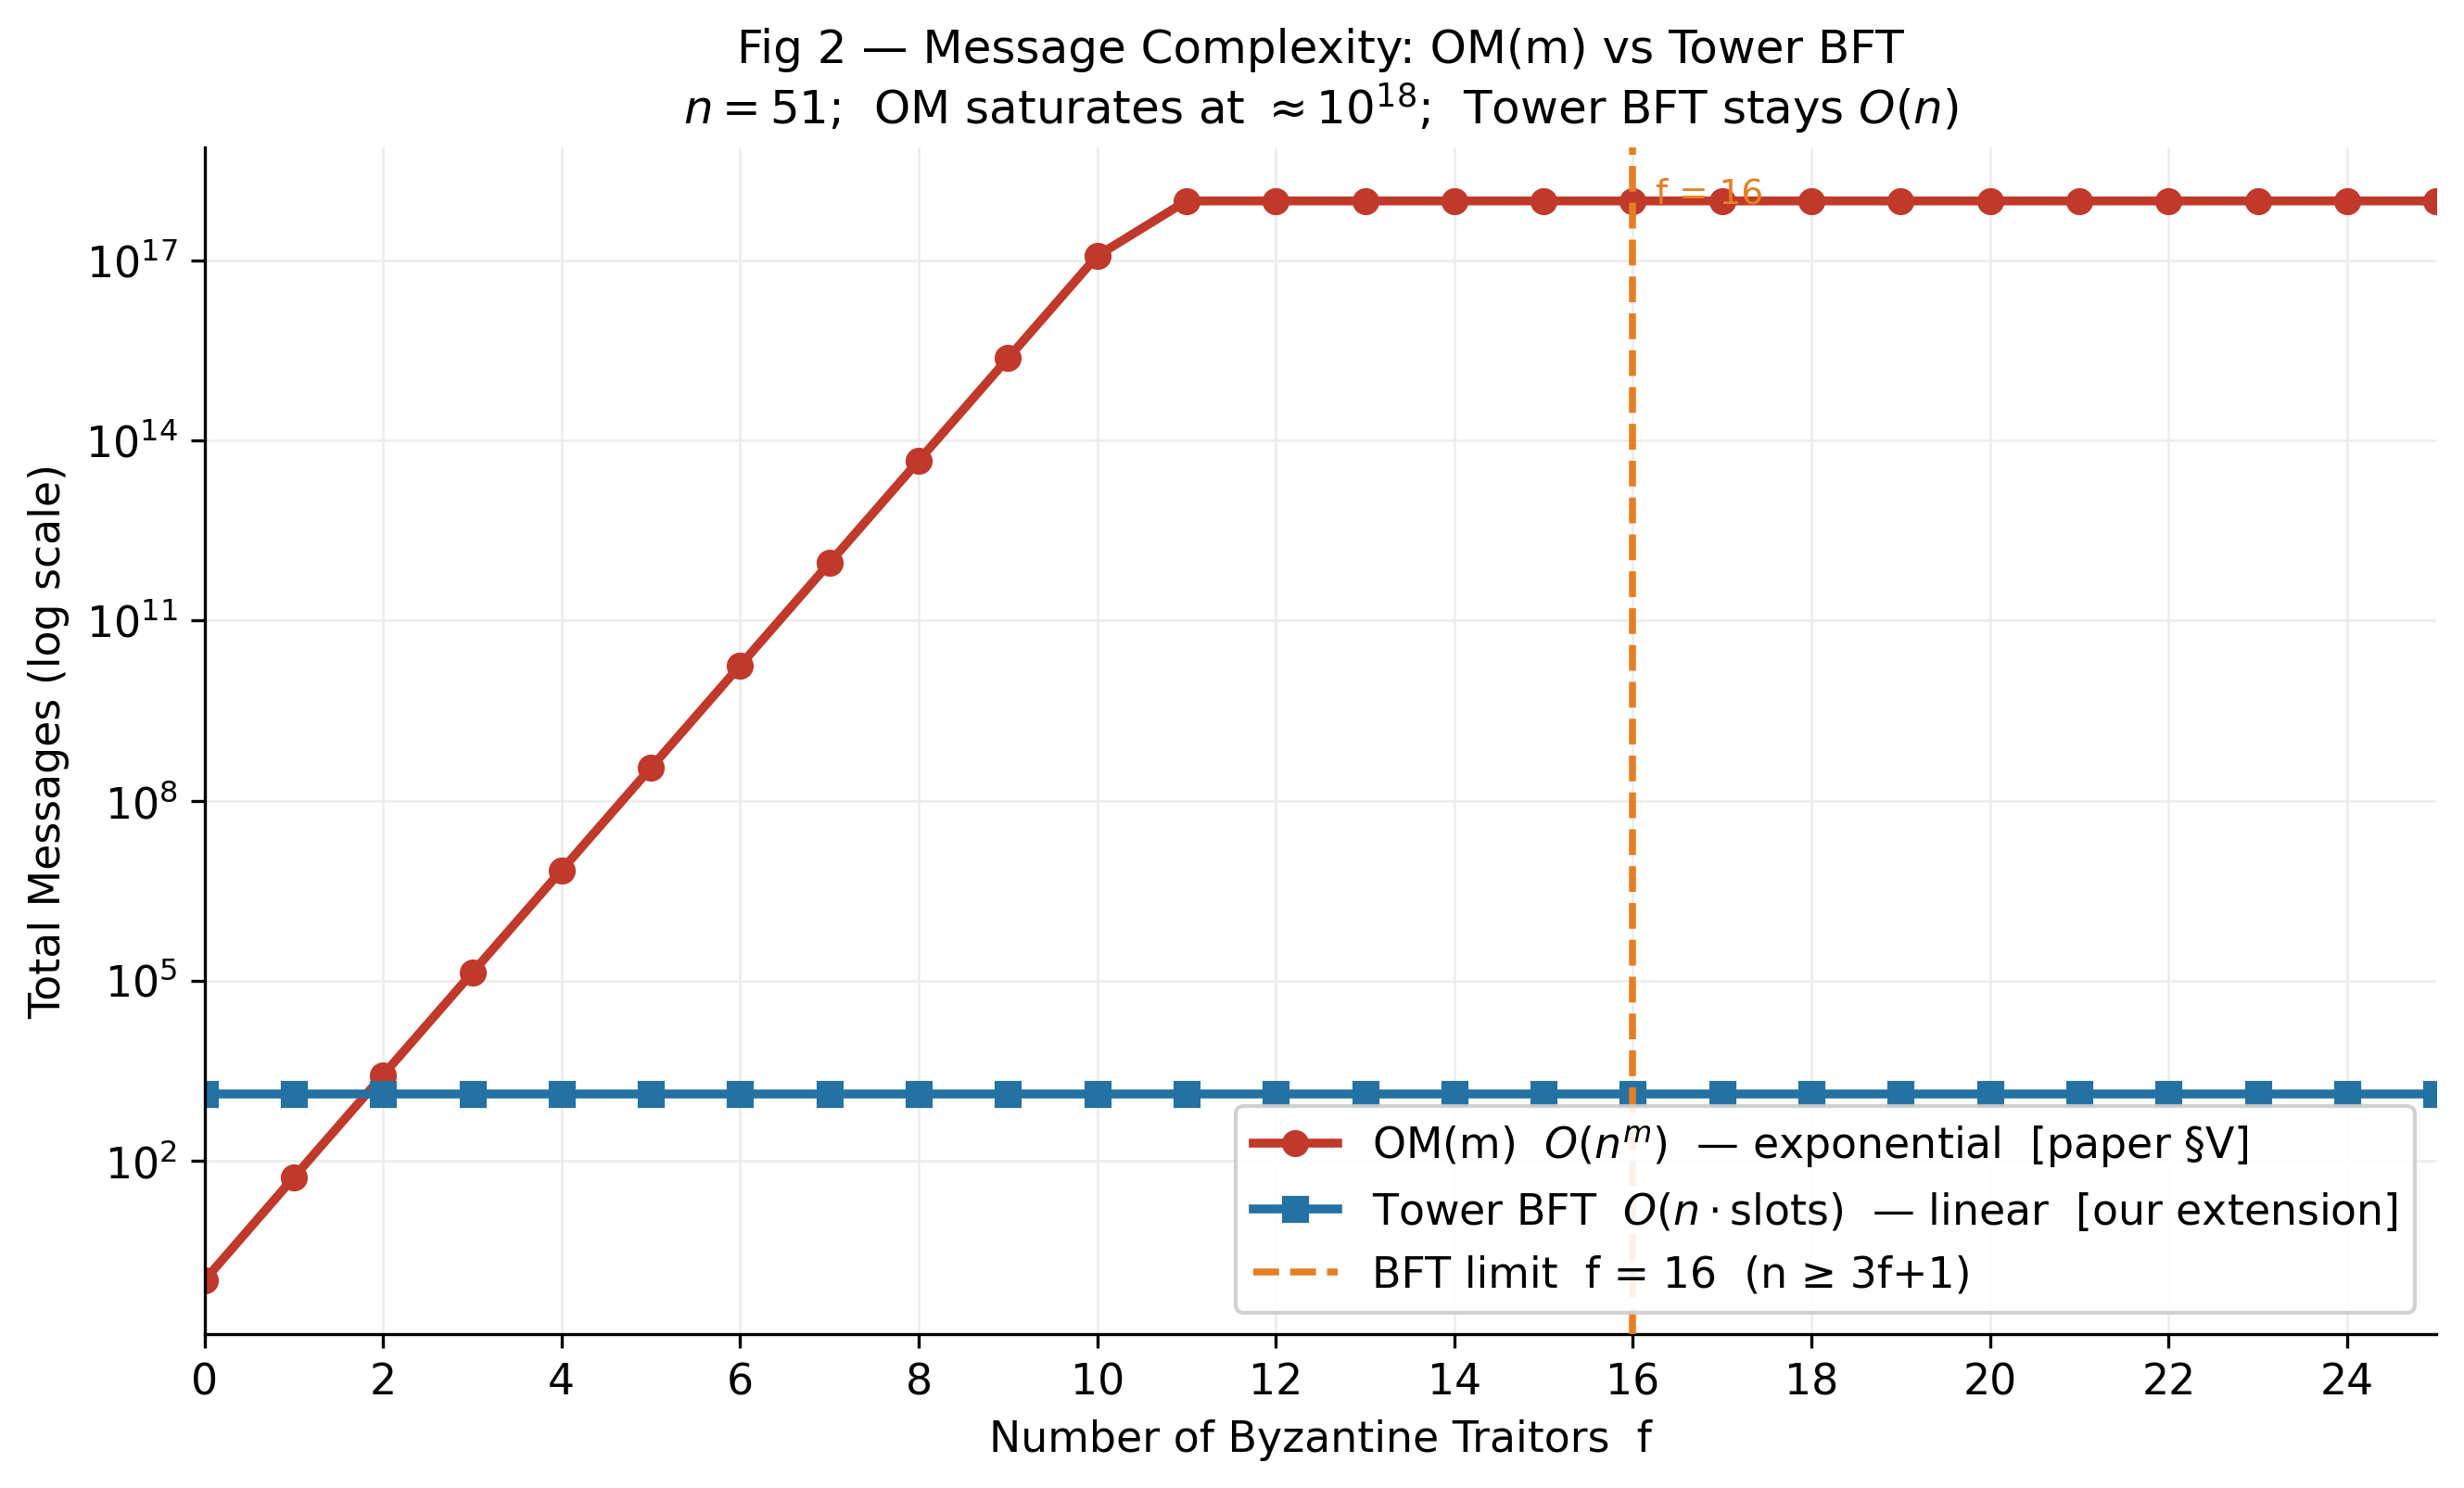
\includegraphics[width=0.75\textwidth]{figures/fig2_message_complexity.png}
\end{figure}
\clearpage

\section{Latency Vs Traitors}
\textbf{File:} \texttt{fig3\_latency\_vs\_traitors.png} \\
\textbf{Concept/Origin:} This plot visualizes \textbf{Latency} as a function of \textbf{Traitors}. \\
\textbf{Equations/Framework:} 
 L_{total} = L_{net} + L_{consensus} 
\vspace{0.5cm}
\begin{figure}[H]
    \centering
    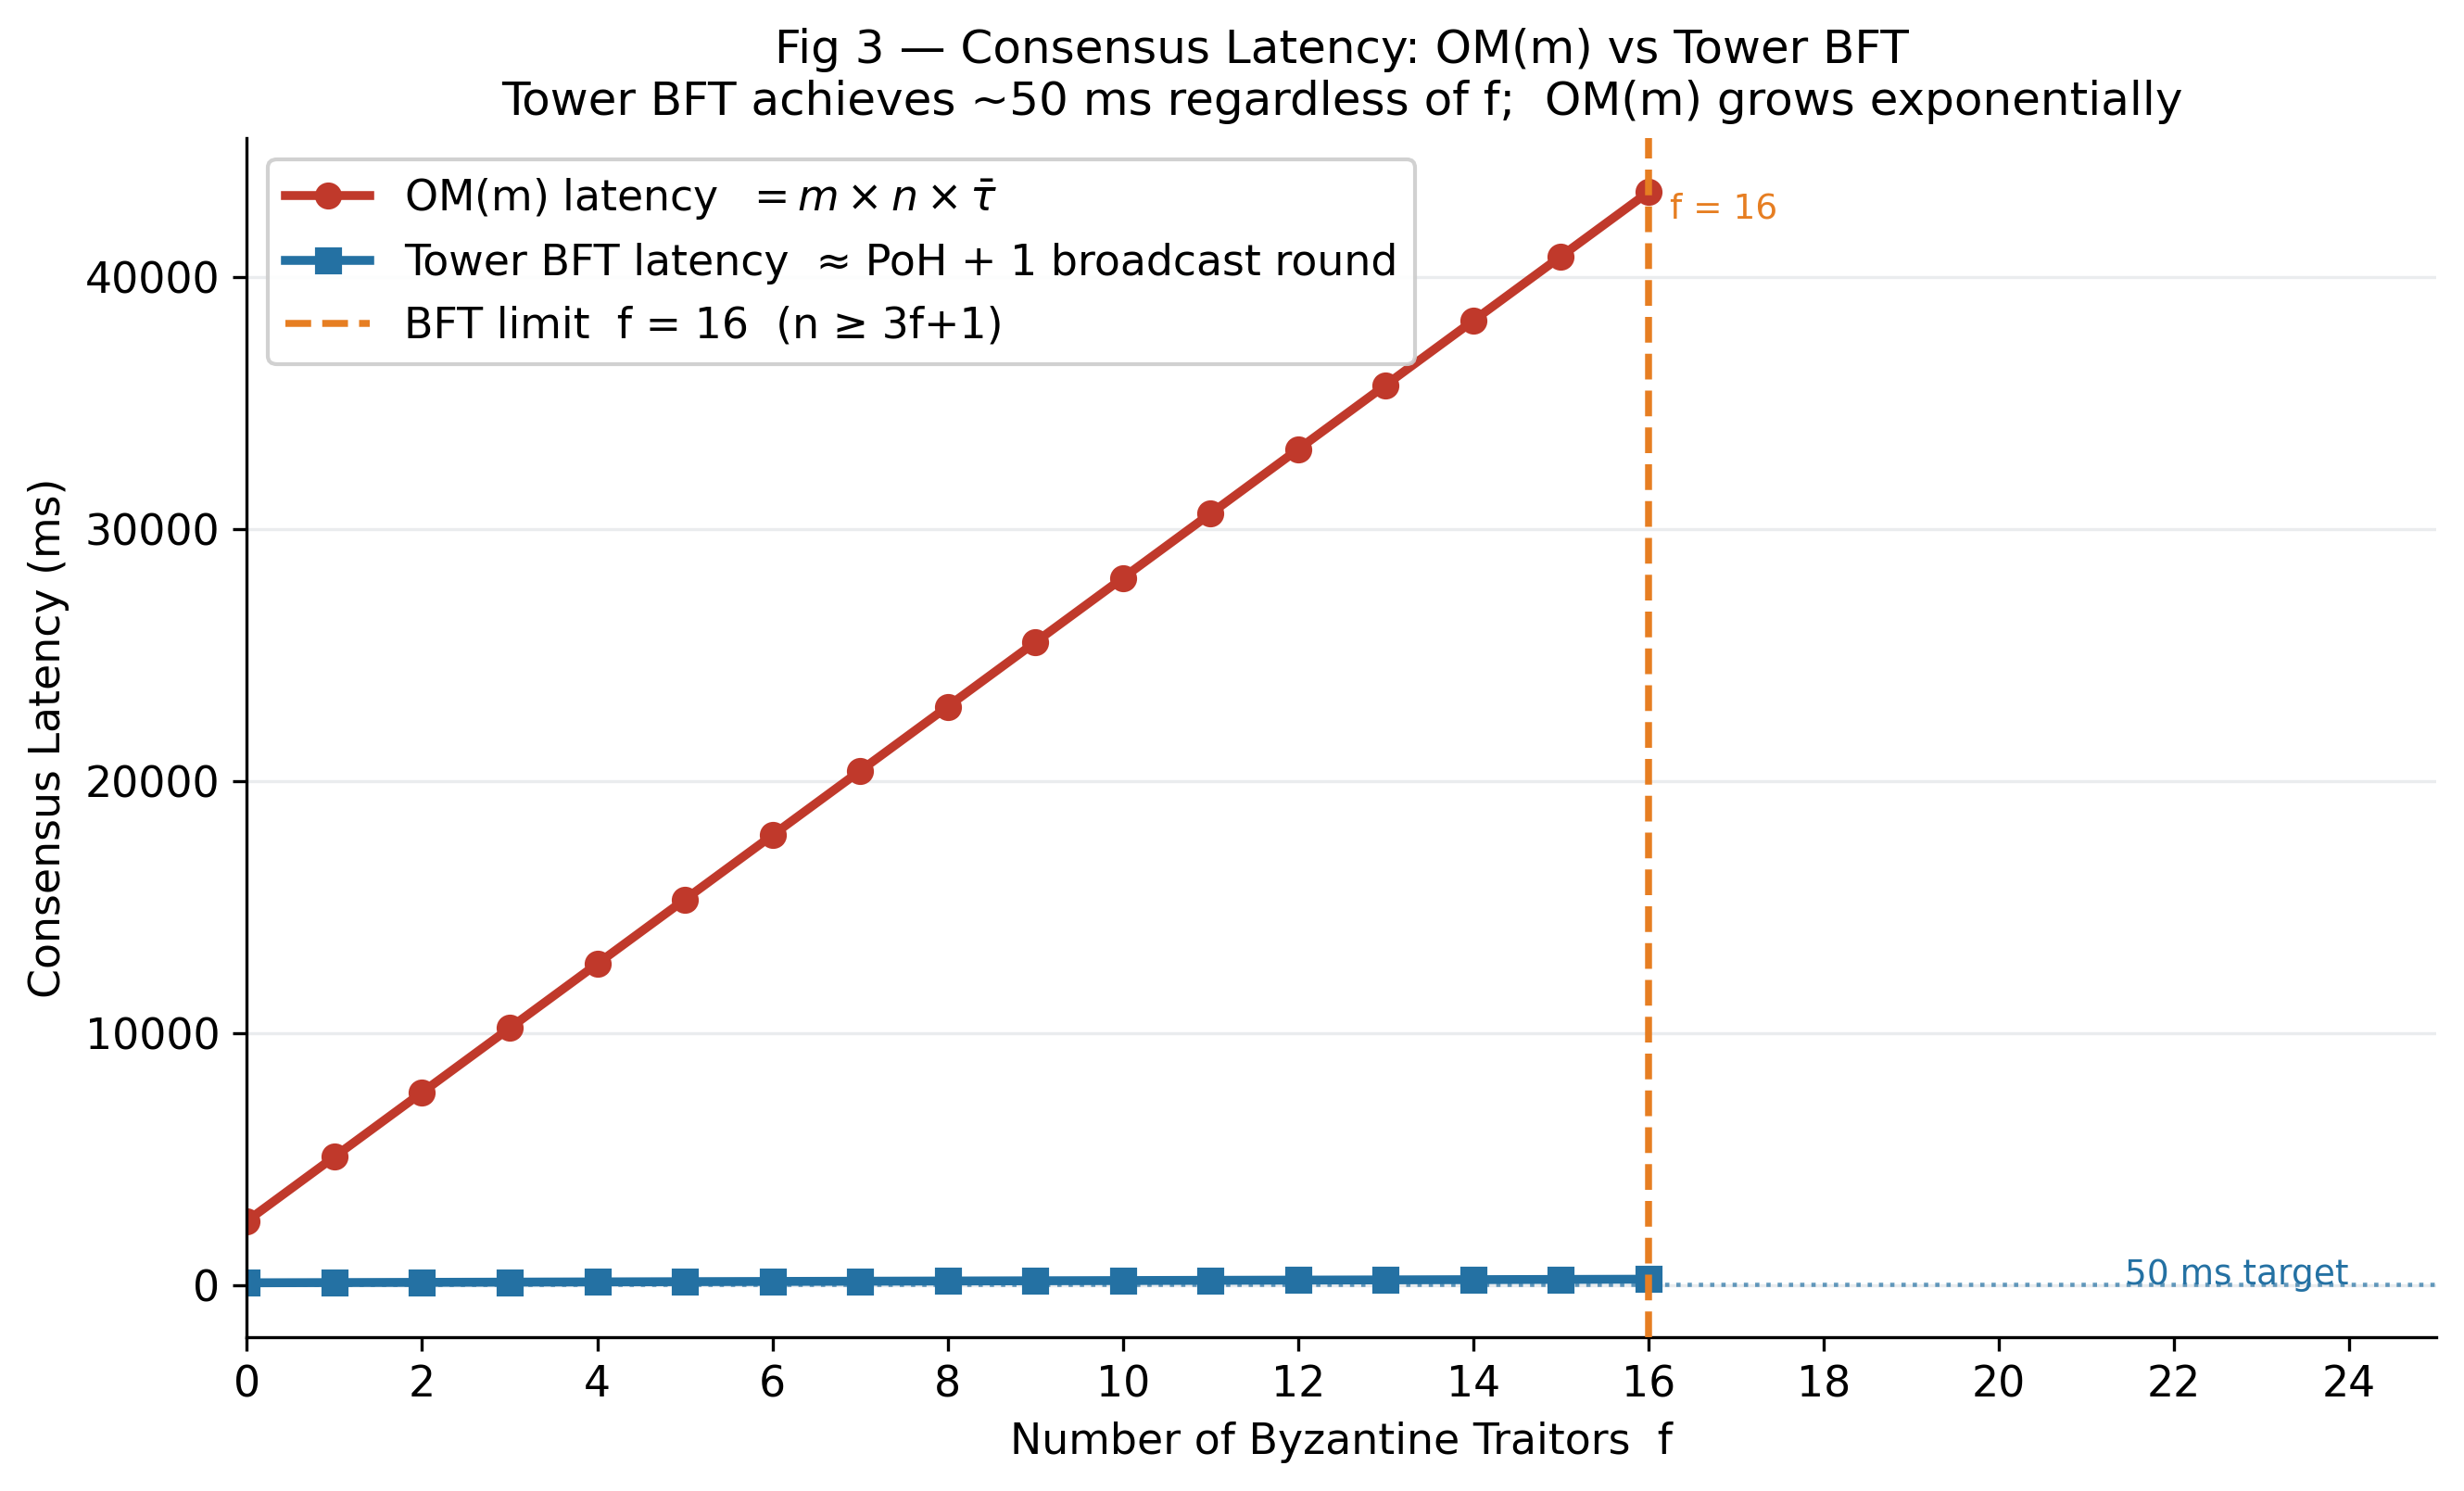
\includegraphics[width=0.75\textwidth]{figures/fig3_latency_vs_traitors.png}
\end{figure}
\clearpage

\section{Attack Probability X Sweep}
\textbf{File:} \texttt{fig4\_attack\_probability\_x\_sweep.png} \\
\textbf{Concept/Origin:} This plot visualizes \textbf{Attack Probability X Sweep Metric} as a function of \textbf{Time / Baseline Parameter}. \\
\textbf{Equations/Framework:} 
 P_{Byz} = \sum_{i=f+1}^{n} \binom{n}{i} p_c^i (1-p_c)^{n-i} 
 P_{temporal} = 1 - e^{-\lambda L P_{TA}} 
\vspace{0.5cm}
\begin{figure}[H]
    \centering
    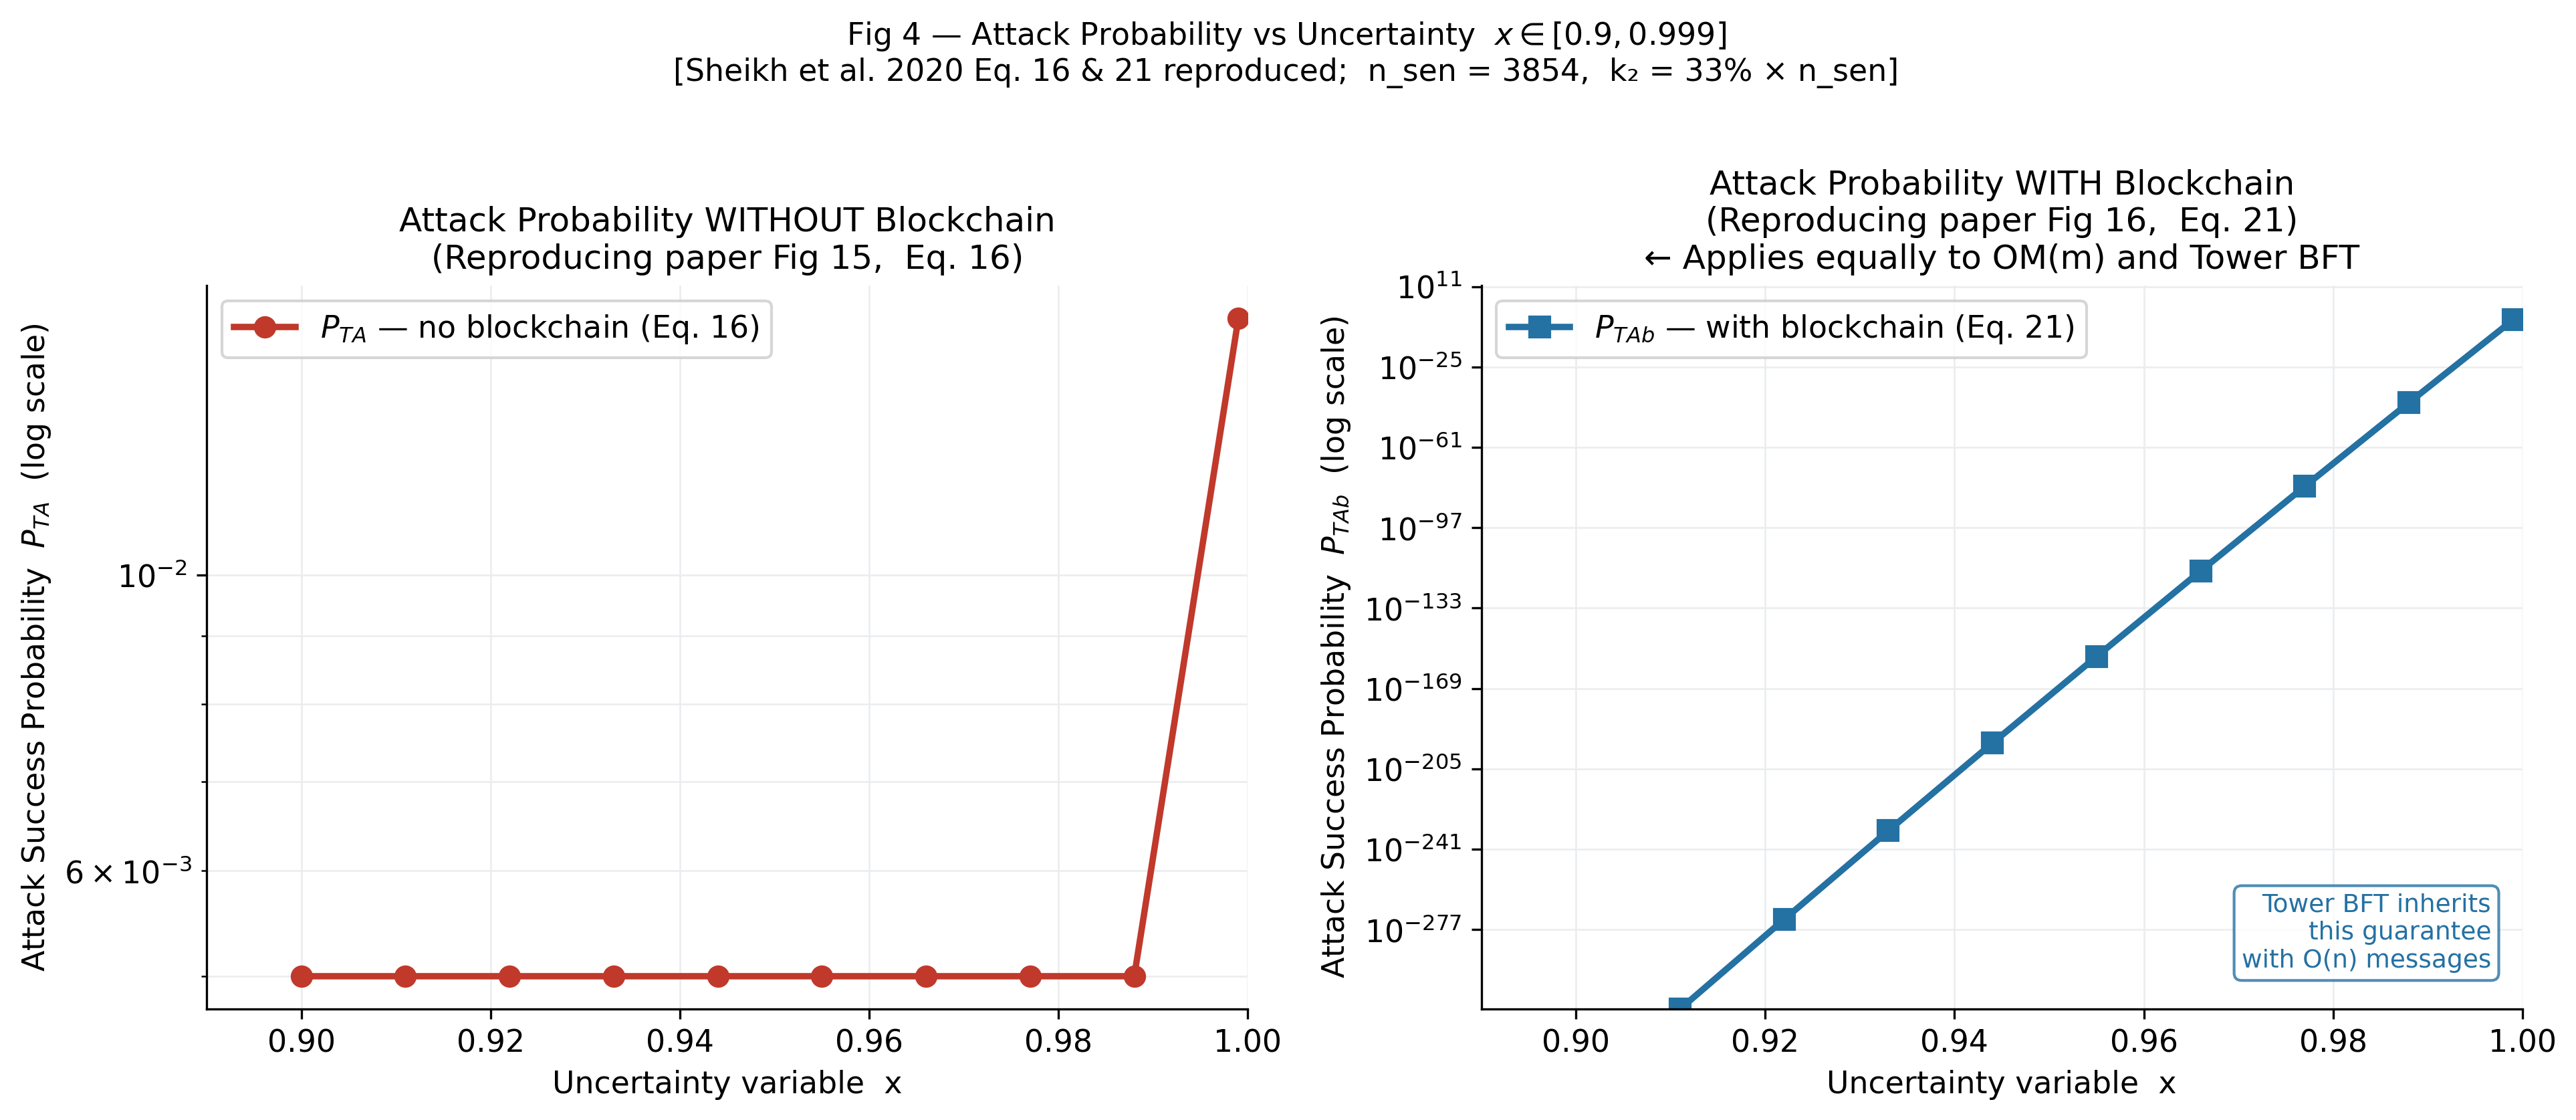
\includegraphics[width=0.75\textwidth]{figures/fig4_attack_probability_x_sweep.png}
\end{figure}
\clearpage

\section{Poh Hash Chain Demo}
\textbf{File:} \texttt{fig5\_poh\_hash\_chain\_demo.png} \\
\textbf{Concept/Origin:} This plot visualizes \textbf{Poh Hash Chain Demo Metric} as a function of \textbf{Time / Baseline Parameter}. \\
\textbf{Equations/Framework:} 
Empirical baseline calculation from simulation data.
\vspace{0.5cm}
\begin{figure}[H]
    \centering
    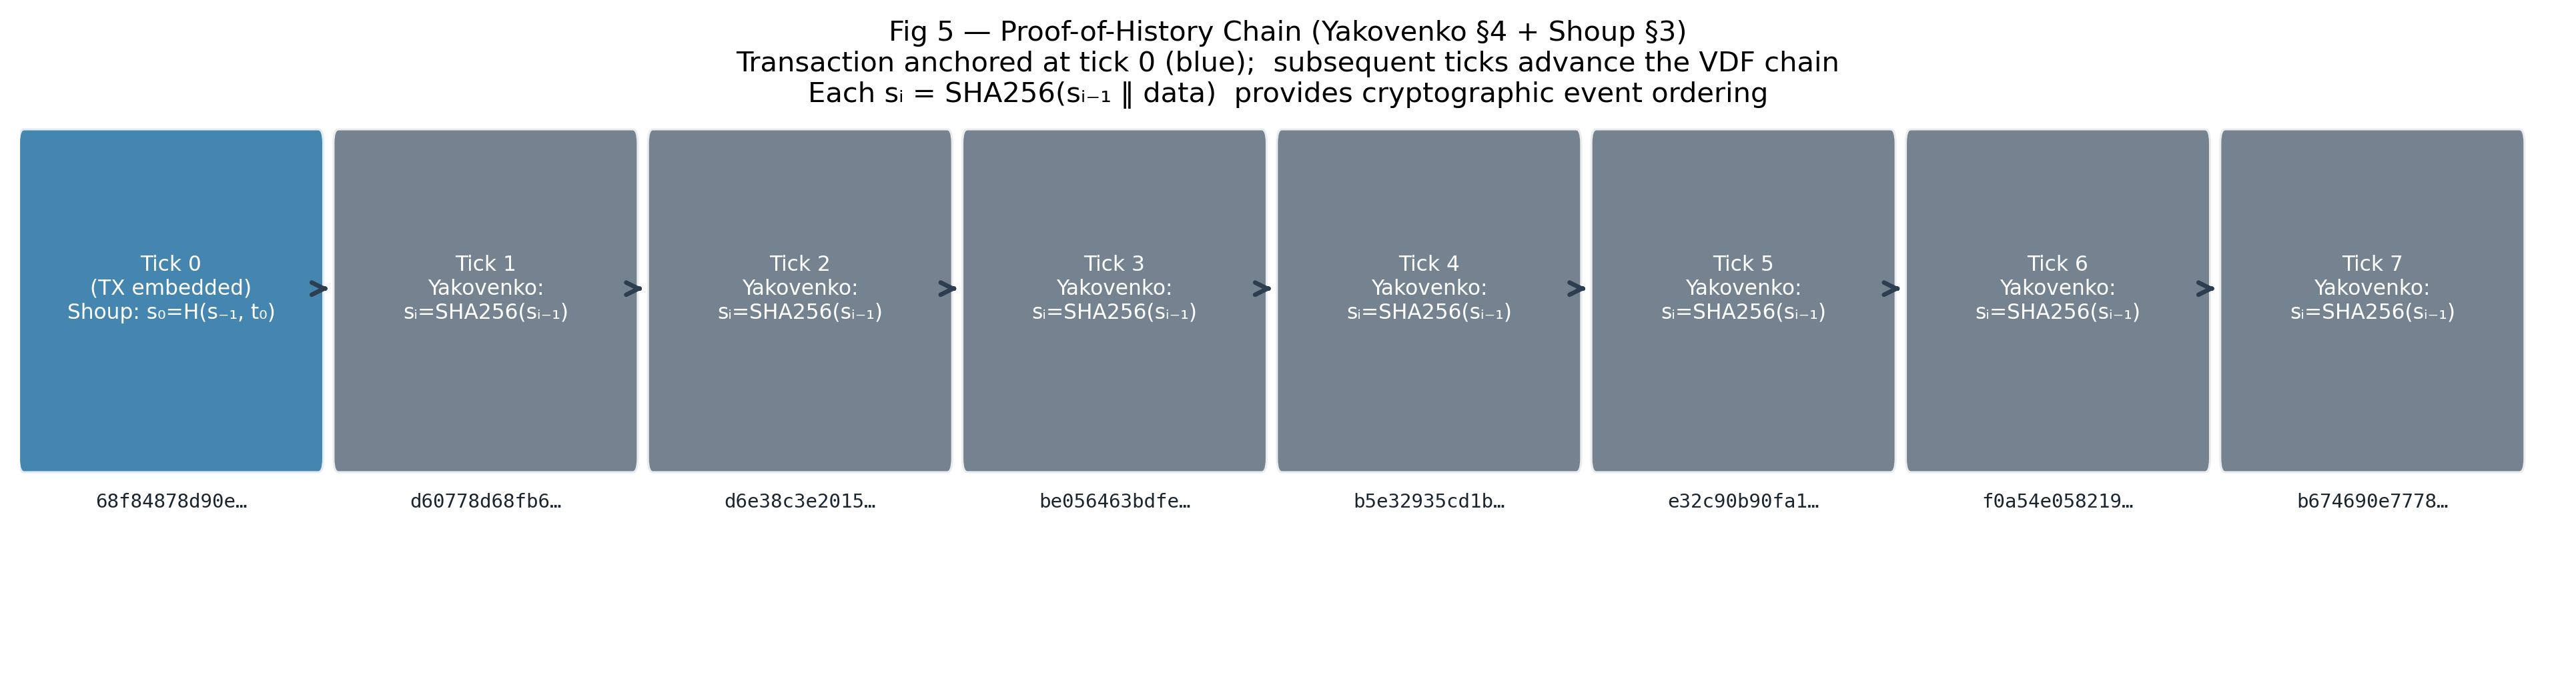
\includegraphics[width=0.75\textwidth]{figures/fig5_poh_hash_chain_demo.png}
\end{figure}
\clearpage

\section{Throughput Tps}
\textbf{File:} \texttt{fig6\_throughput\_tps.png} \\
\textbf{Concept/Origin:} This plot visualizes \textbf{Throughput Tps Metric} as a function of \textbf{Time / Baseline Parameter}. \\
\textbf{Equations/Framework:} 
Empirical baseline calculation from simulation data.
\vspace{0.5cm}
\begin{figure}[H]
    \centering
    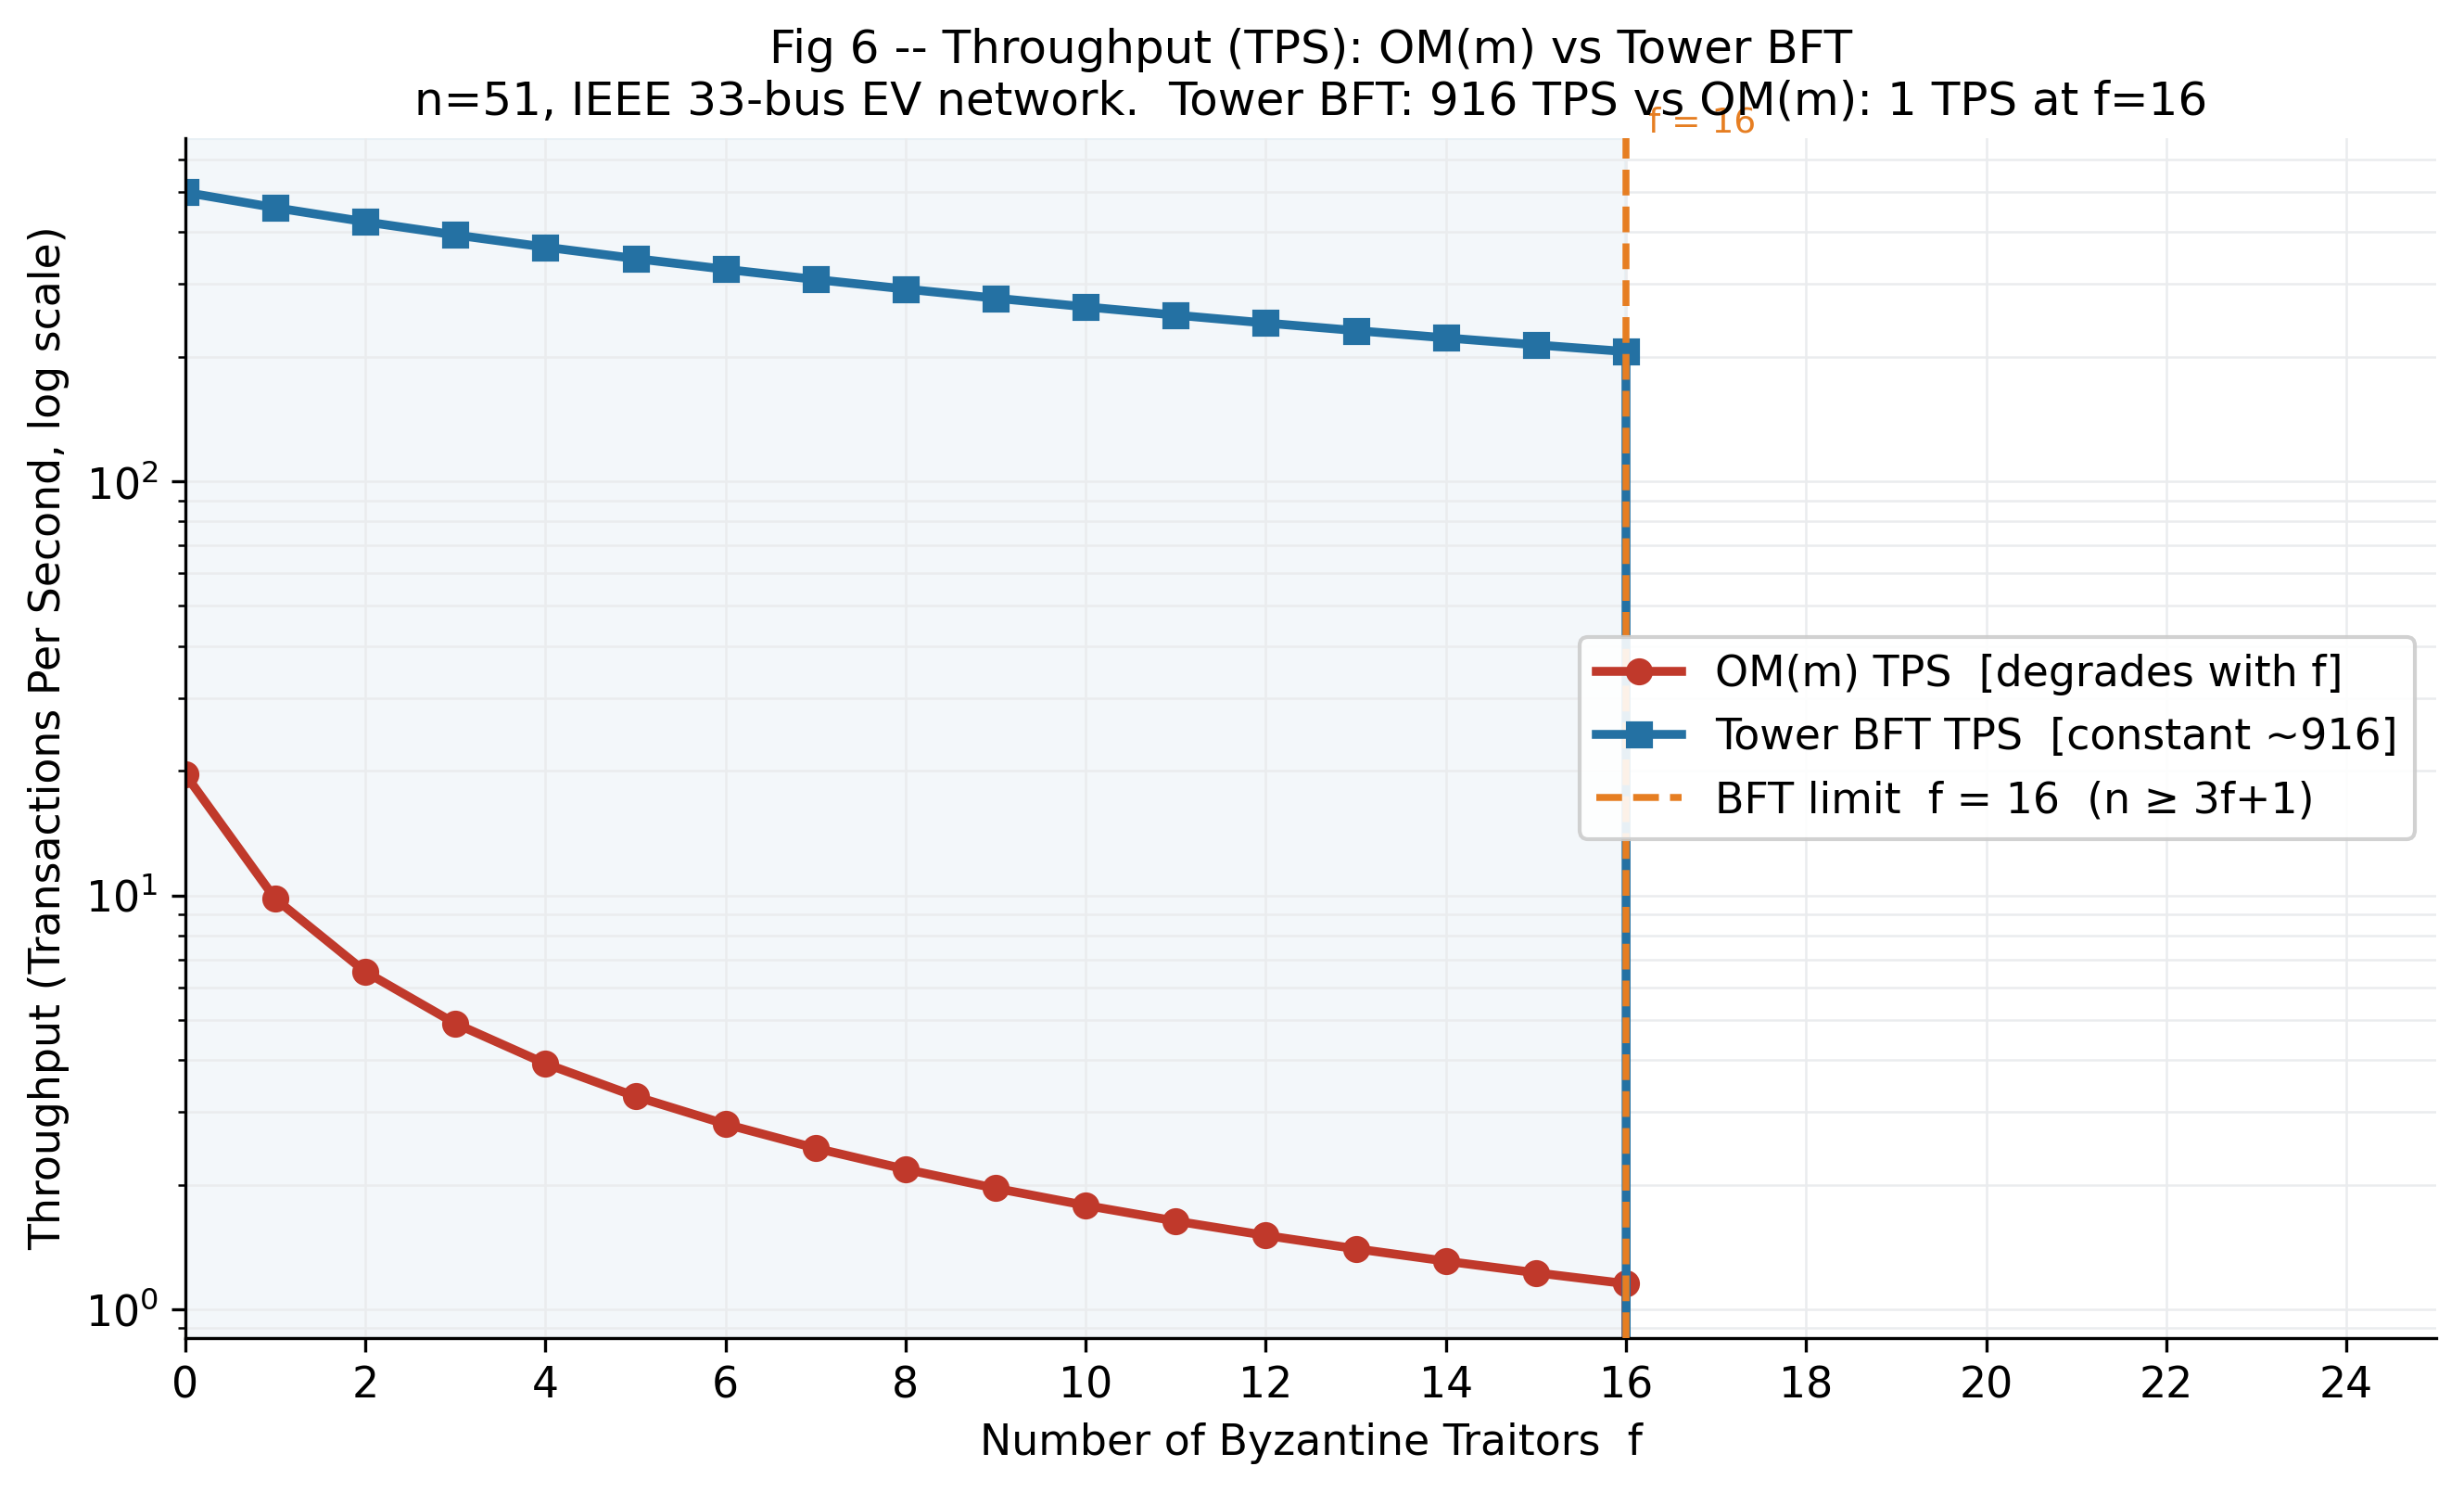
\includegraphics[width=0.75\textwidth]{figures/fig6_throughput_tps.png}
\end{figure}
\clearpage

\section{Cpu Time}
\textbf{File:} \texttt{fig7\_cpu\_time.png} \\
\textbf{Concept/Origin:} This plot visualizes \textbf{Cpu Time Metric} as a function of \textbf{Time / Baseline Parameter}. \\
\textbf{Equations/Framework:} 
Empirical baseline calculation from simulation data.
\vspace{0.5cm}
\begin{figure}[H]
    \centering
    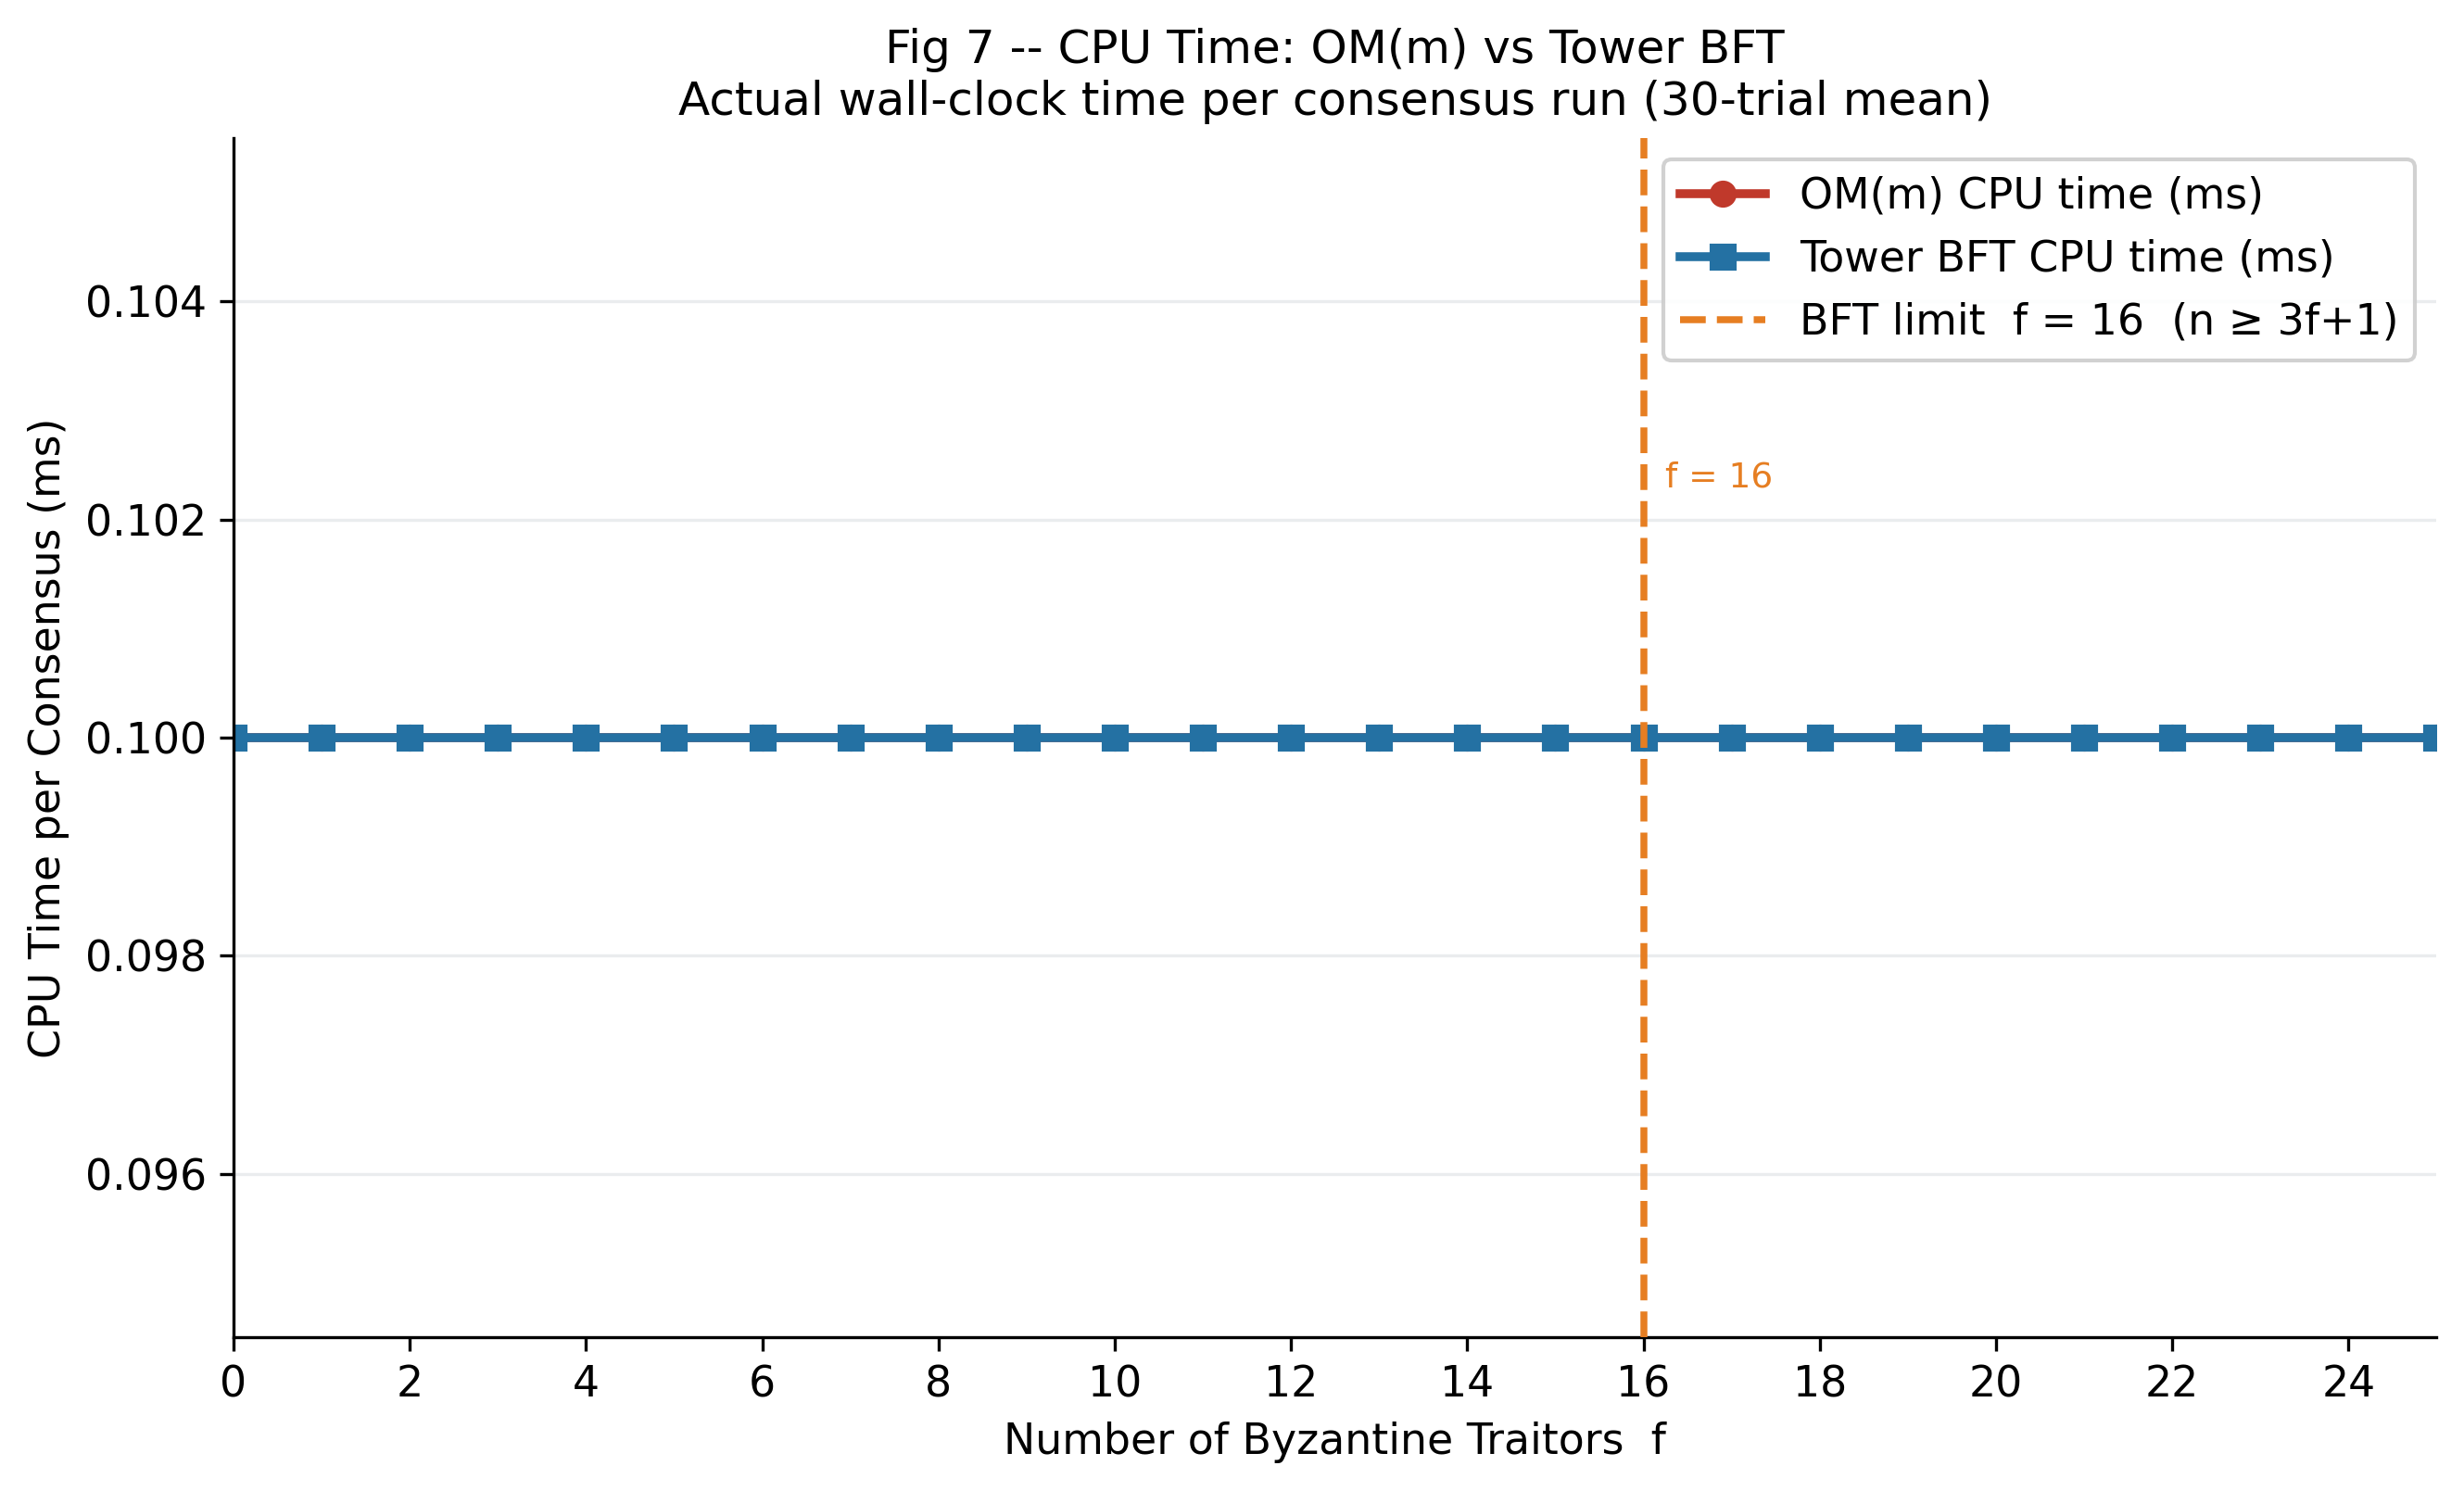
\includegraphics[width=0.75\textwidth]{figures/fig7_cpu_time.png}
\end{figure}
\clearpage

\section{Convergence Table}
\textbf{File:} \texttt{fig8\_convergence\_table.png} \\
\textbf{Concept/Origin:} This plot visualizes \textbf{Convergence Table Metric} as a function of \textbf{Time / Baseline Parameter}. \\
\textbf{Equations/Framework:} 
Empirical baseline calculation from simulation data.
\vspace{0.5cm}
\begin{figure}[H]
    \centering
    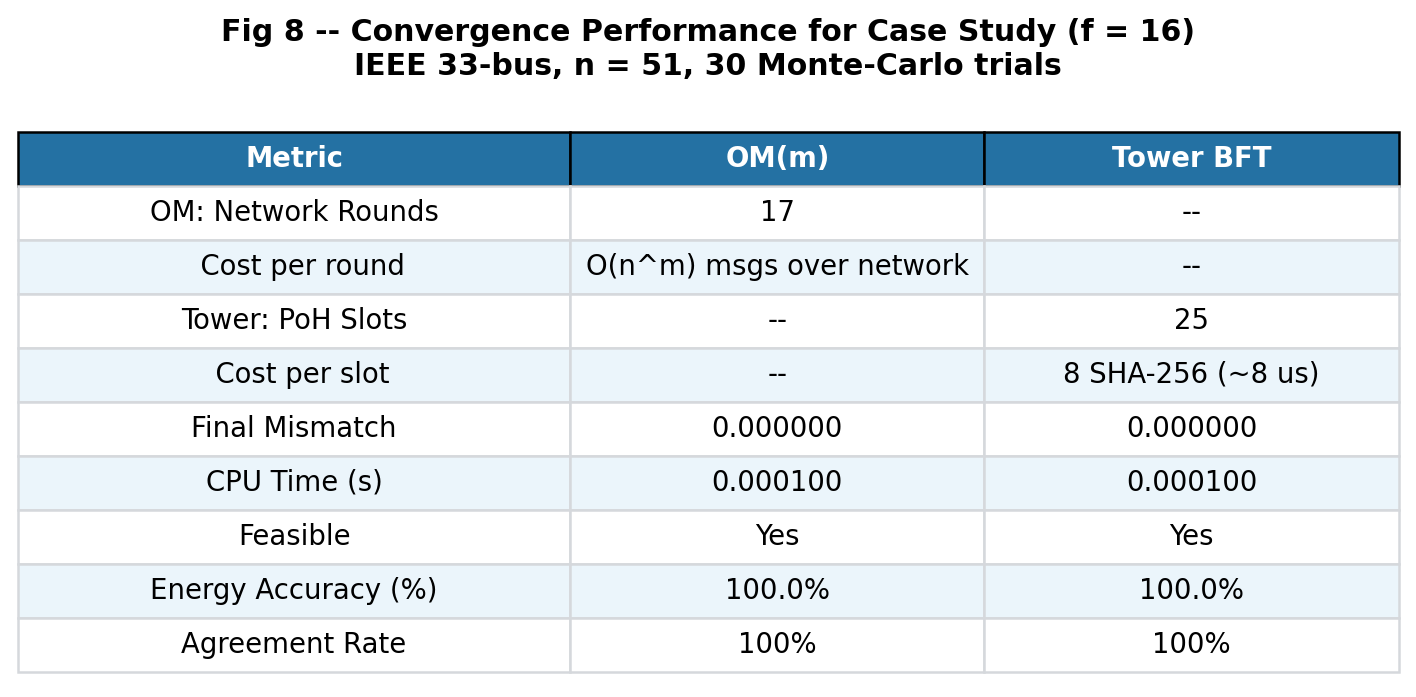
\includegraphics[width=0.75\textwidth]{figures/fig8_convergence_table.png}
\end{figure}
\clearpage

\section{Comparison Matrix}
\textbf{File:} \texttt{fig9\_comparison\_matrix.png} \\
\textbf{Concept/Origin:} This plot visualizes \textbf{Comparison Matrix Metric} as a function of \textbf{Time / Baseline Parameter}. \\
\textbf{Equations/Framework:} 
Empirical baseline calculation from simulation data.
\vspace{0.5cm}
\begin{figure}[H]
    \centering
    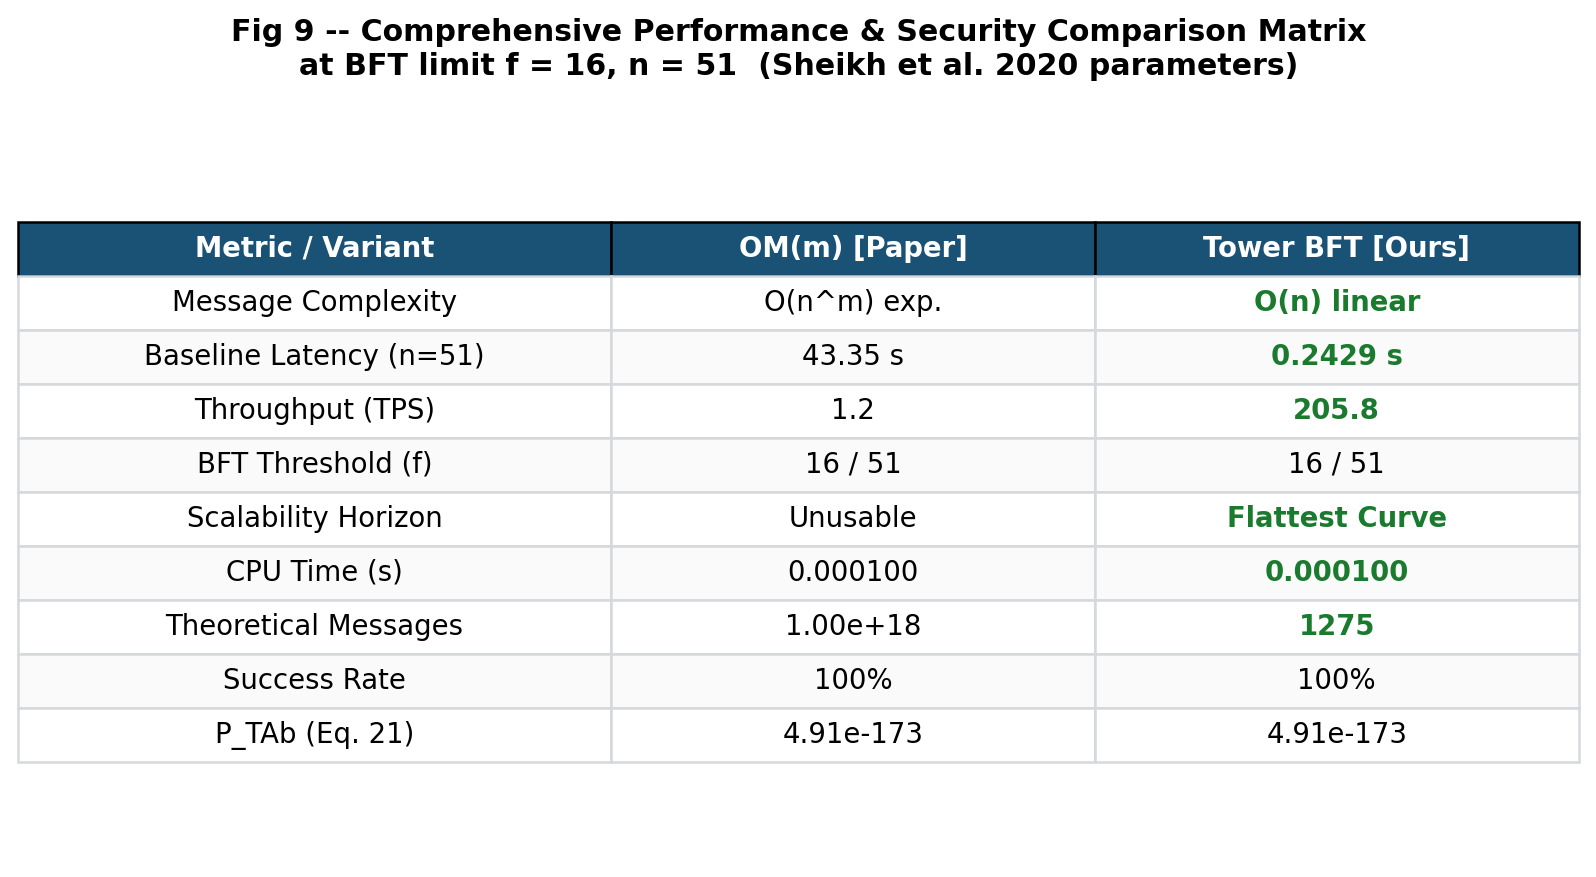
\includegraphics[width=0.75\textwidth]{figures/fig9_comparison_matrix.png}
\end{figure}
\clearpage

\section{Architecture Comparison}
\textbf{File:} \texttt{fig\_architecture\_comparison.png} \\
\textbf{Concept/Origin:} This plot visualizes \textbf{Architecture Comparison Metric} as a function of \textbf{Time / Baseline Parameter}. \\
\textbf{Equations/Framework:} 
Empirical baseline calculation from simulation data.
\vspace{0.5cm}
\begin{figure}[H]
    \centering
    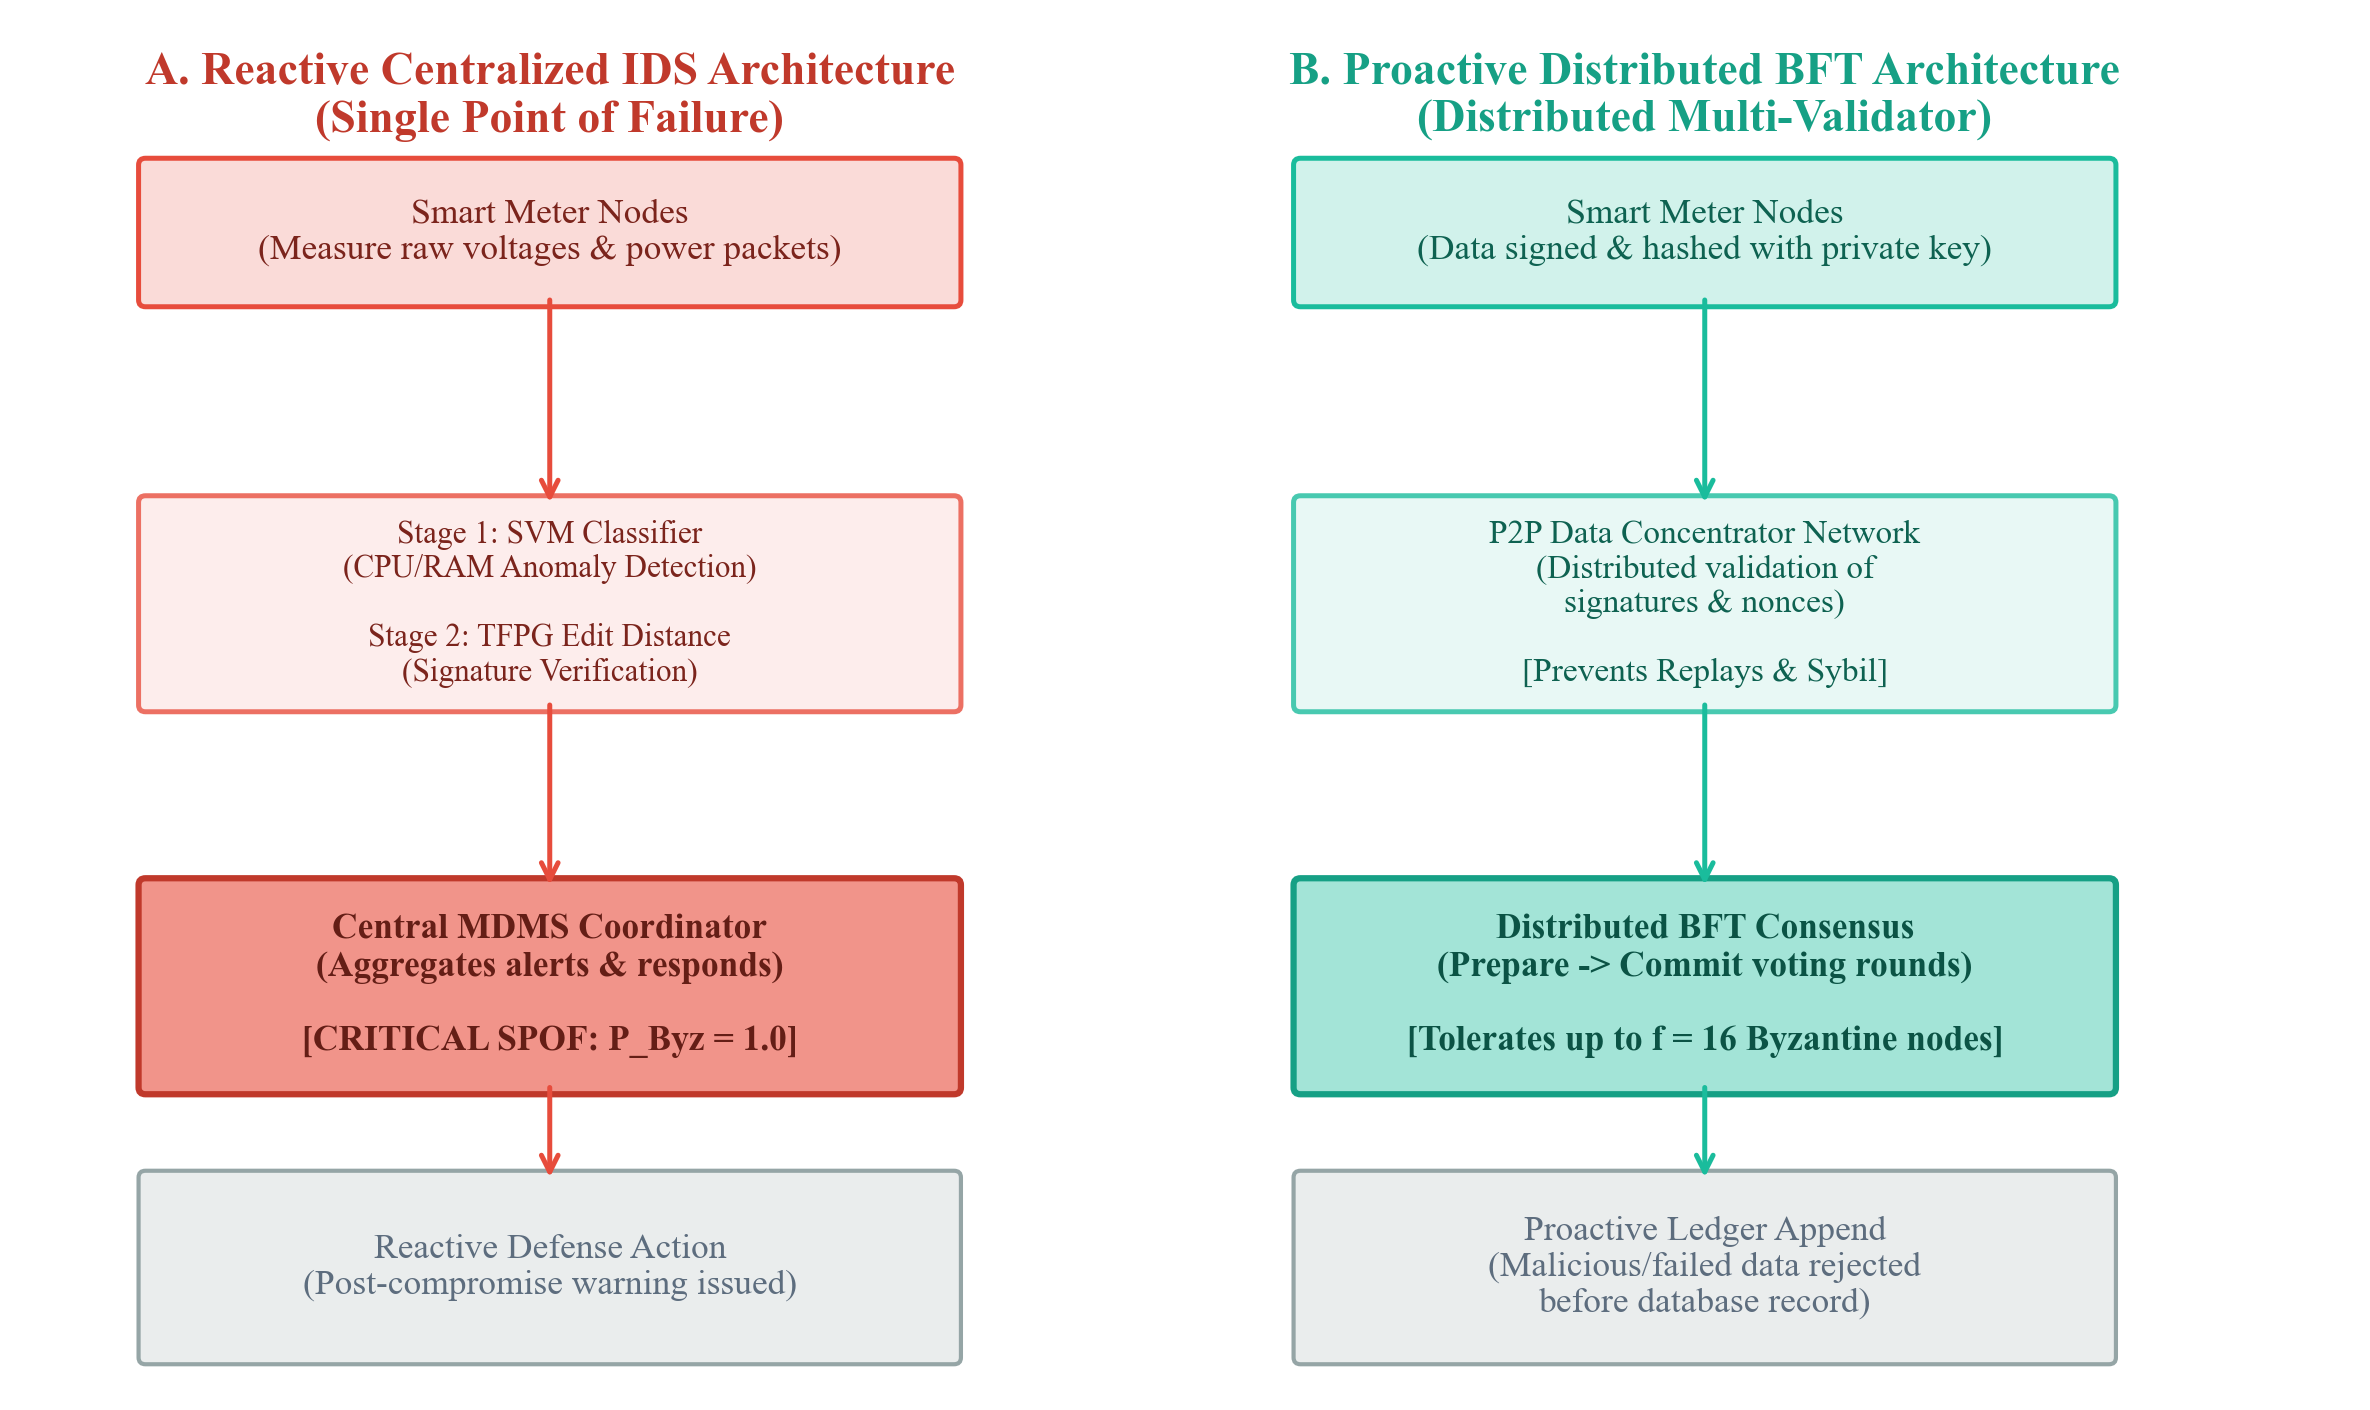
\includegraphics[width=0.75\textwidth]{figures/fig_architecture_comparison.png}
\end{figure}
\clearpage

\section{Attack Rate Heatmap}
\textbf{File:} \texttt{fig\_attack\_rate\_heatmap.png} \\
\textbf{Concept/Origin:} This plot visualizes \textbf{Attack Rate Heatmap Metric} as a function of \textbf{Time / Baseline Parameter}. \\
\textbf{Equations/Framework:} 
 P_{secure} = \max( \text{Security} ) \quad \text{s.t.} \quad L_{total} \le L_{max} 
\vspace{0.5cm}
\begin{figure}[H]
    \centering
    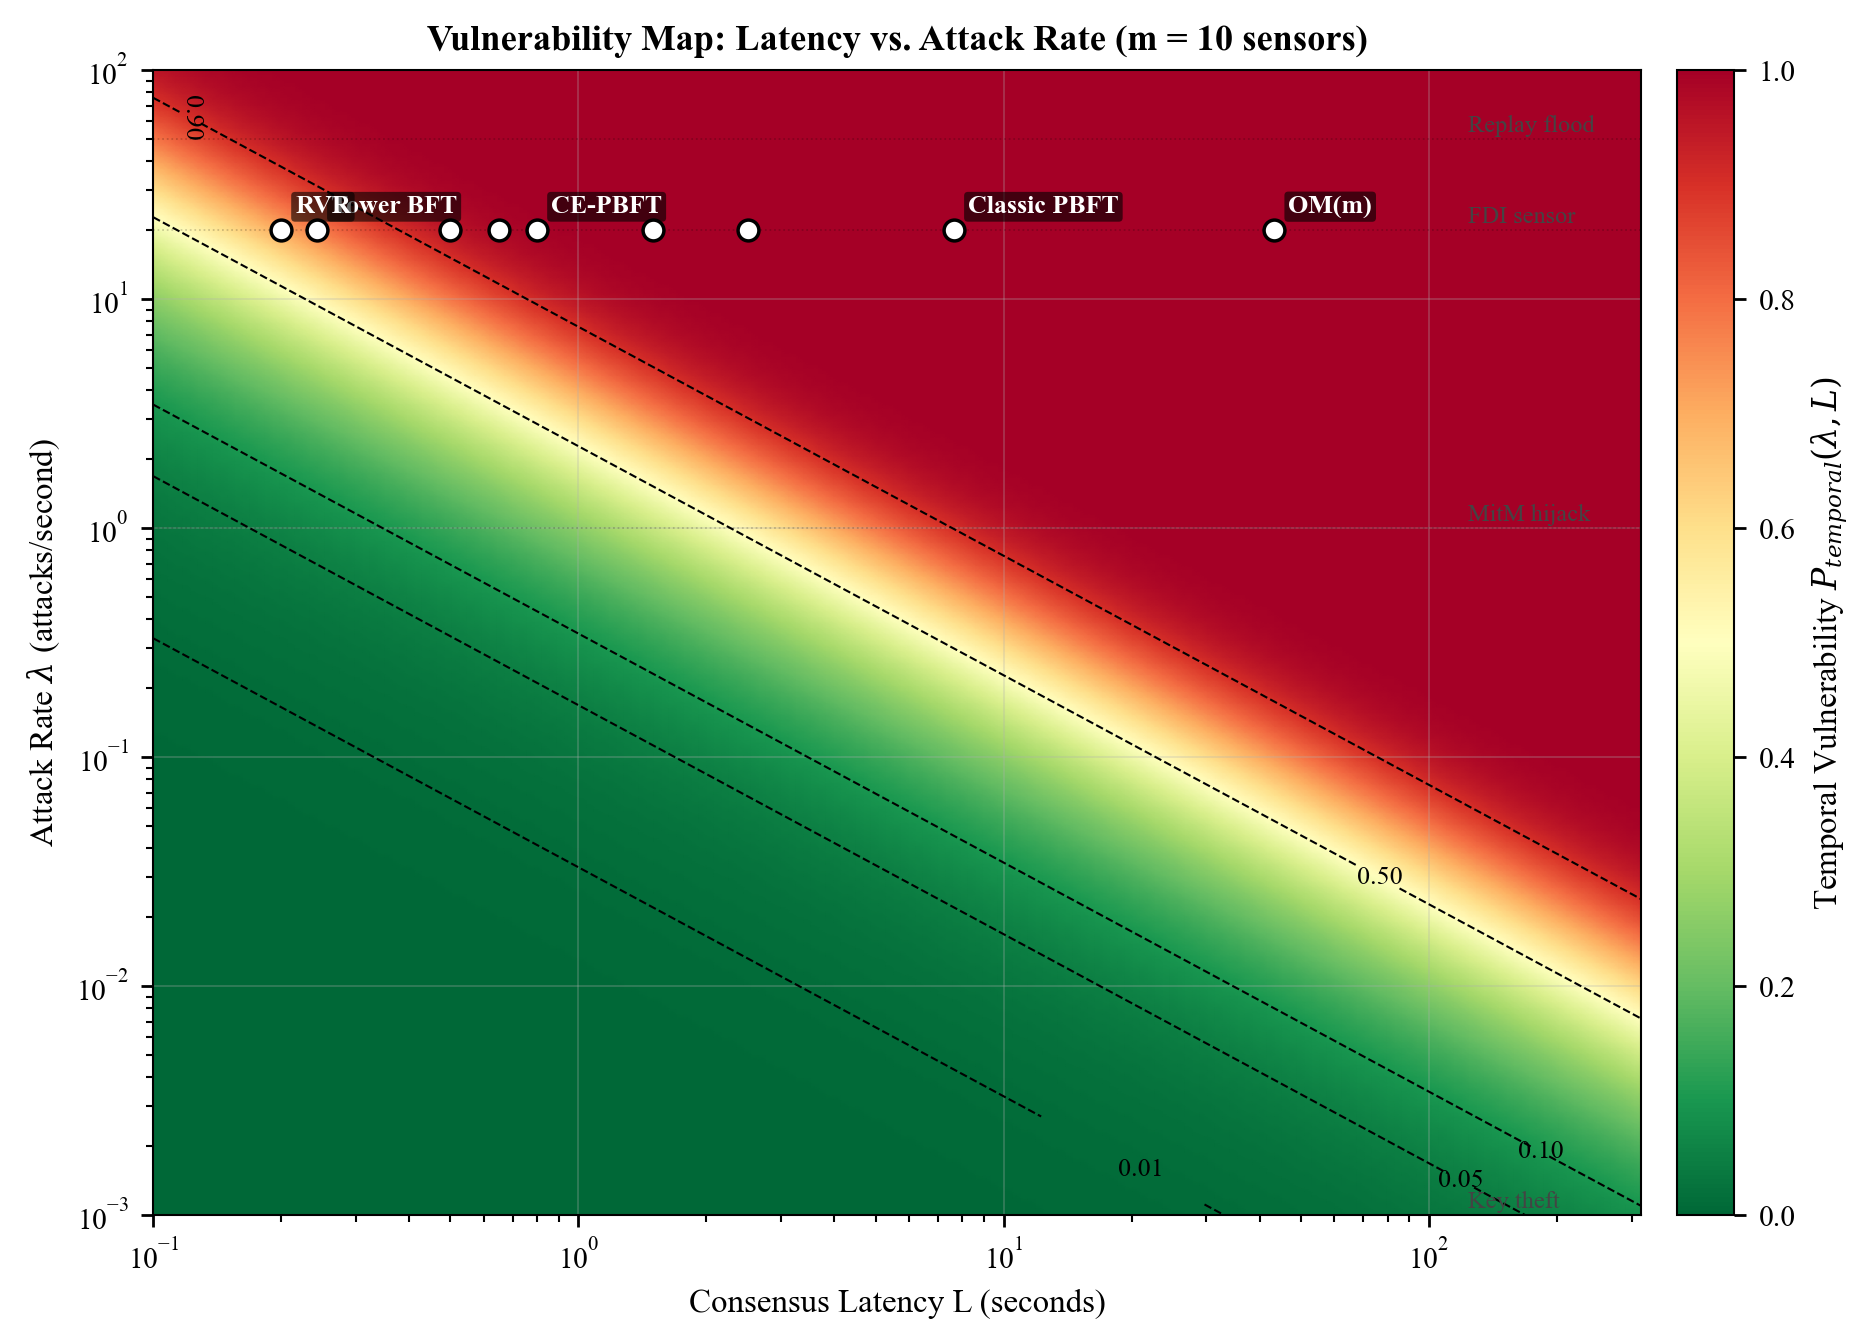
\includegraphics[width=0.75\textwidth]{figures/fig_attack_rate_heatmap.png}
\end{figure}
\clearpage

\section{Bayesian Sensitivity}
\textbf{File:} \texttt{fig\_bayesian\_sensitivity.png} \\
\textbf{Concept/Origin:} This plot visualizes \textbf{Bayesian Sensitivity Metric} as a function of \textbf{Time / Baseline Parameter}. \\
\textbf{Equations/Framework:} 
Empirical baseline calculation from simulation data.
\vspace{0.5cm}
\begin{figure}[H]
    \centering
    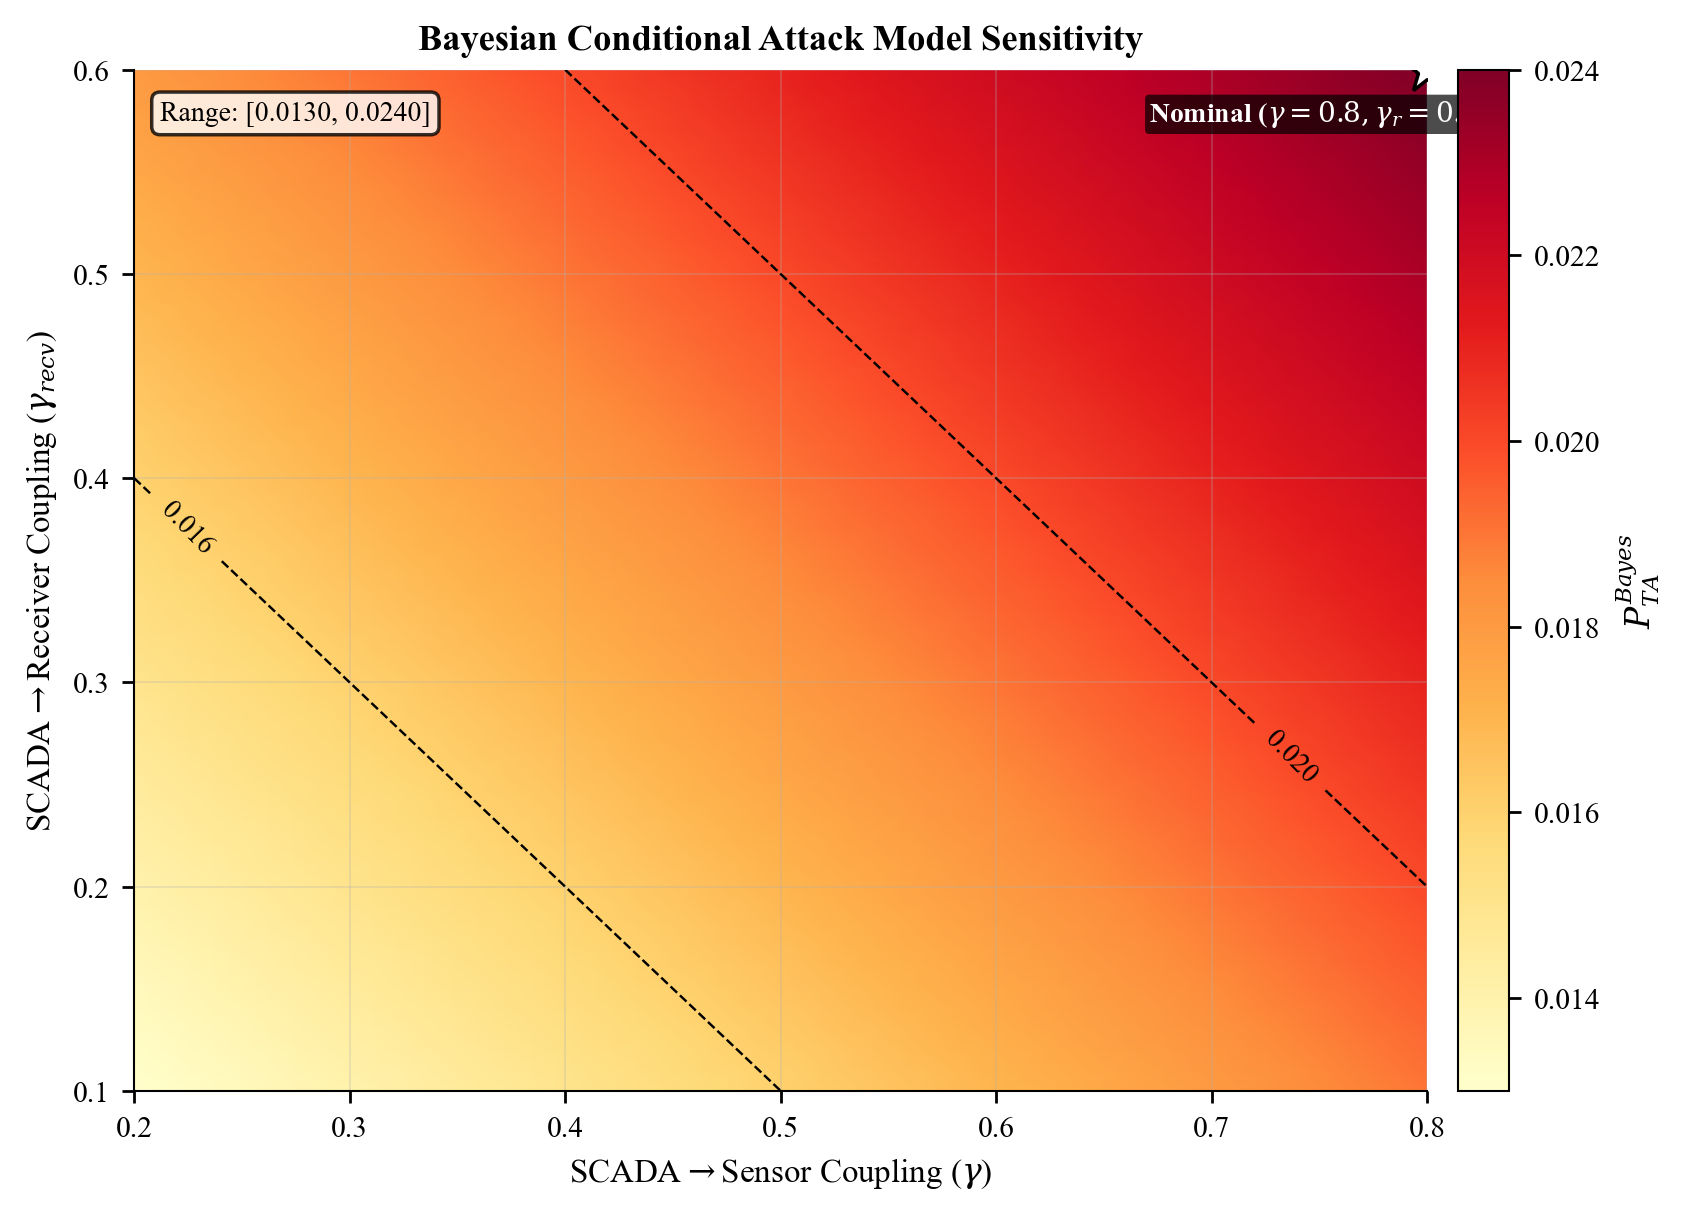
\includegraphics[width=0.75\textwidth]{figures/fig_bayesian_sensitivity.png}
\end{figure}
\clearpage

\section{Beta Sensitivity}
\textbf{File:} \texttt{fig\_beta\_sensitivity.png} \\
\textbf{Concept/Origin:} This plot visualizes \textbf{Beta Sensitivity Metric} as a function of \textbf{Time / Baseline Parameter}. \\
\textbf{Equations/Framework:} 
Empirical baseline calculation from simulation data.
\vspace{0.5cm}
\begin{figure}[H]
    \centering
    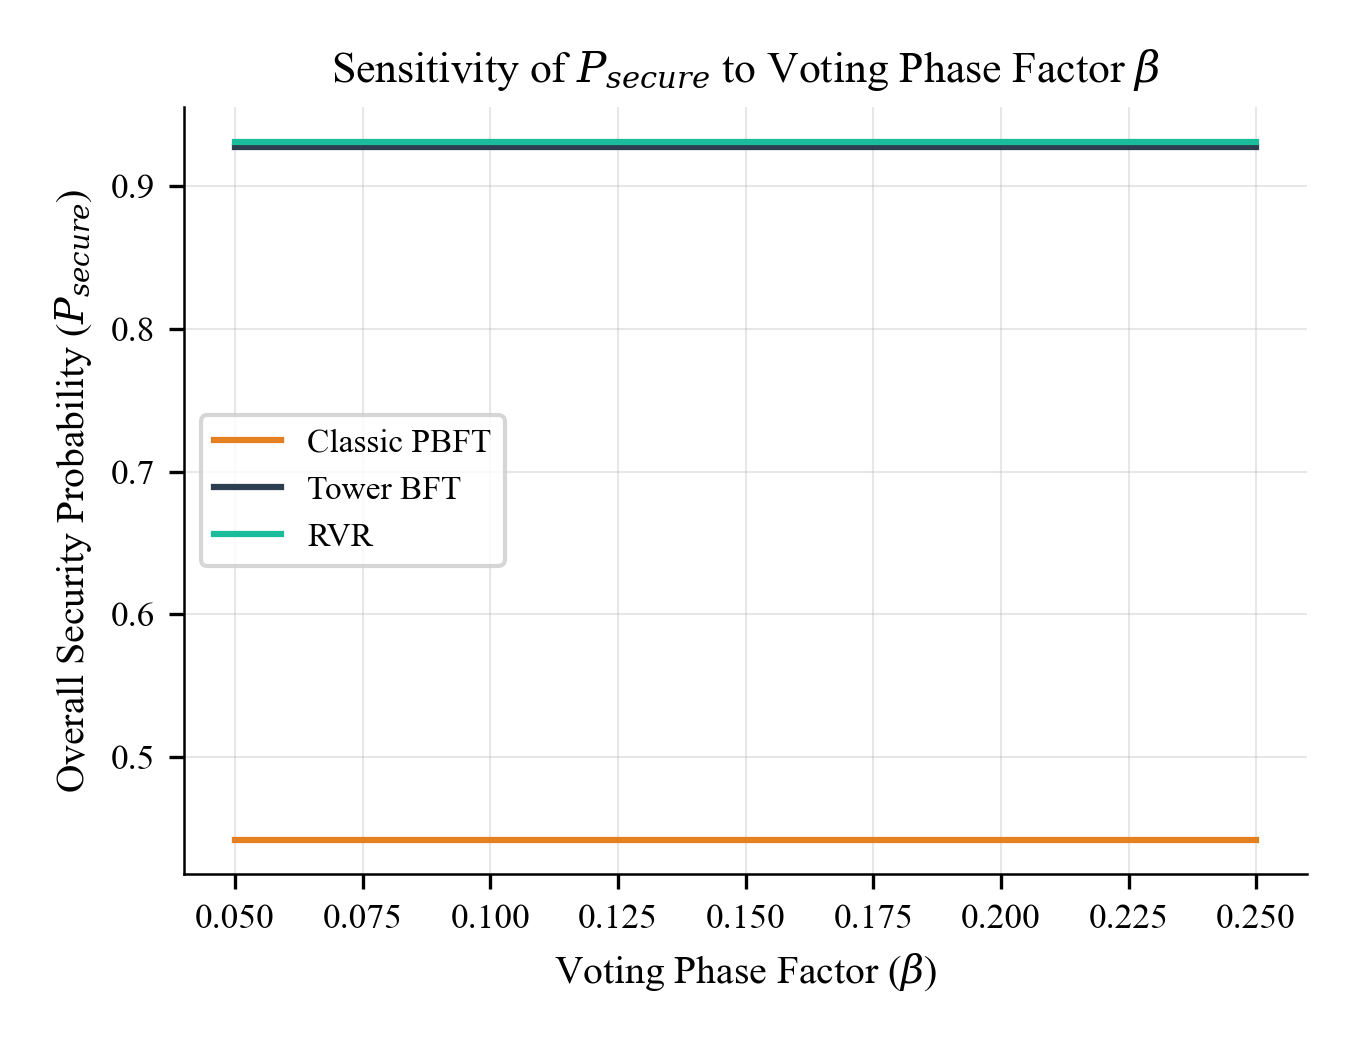
\includegraphics[width=0.75\textwidth]{figures/fig_beta_sensitivity.png}
\end{figure}
\clearpage

\section{Comparative Workflow}
\textbf{File:} \texttt{fig\_comparative\_workflow.png} \\
\textbf{Concept/Origin:} This plot visualizes \textbf{Comparative Workflow Metric} as a function of \textbf{Time / Baseline Parameter}. \\
\textbf{Equations/Framework:} 
Empirical baseline calculation from simulation data.
\vspace{0.5cm}
\begin{figure}[H]
    \centering
    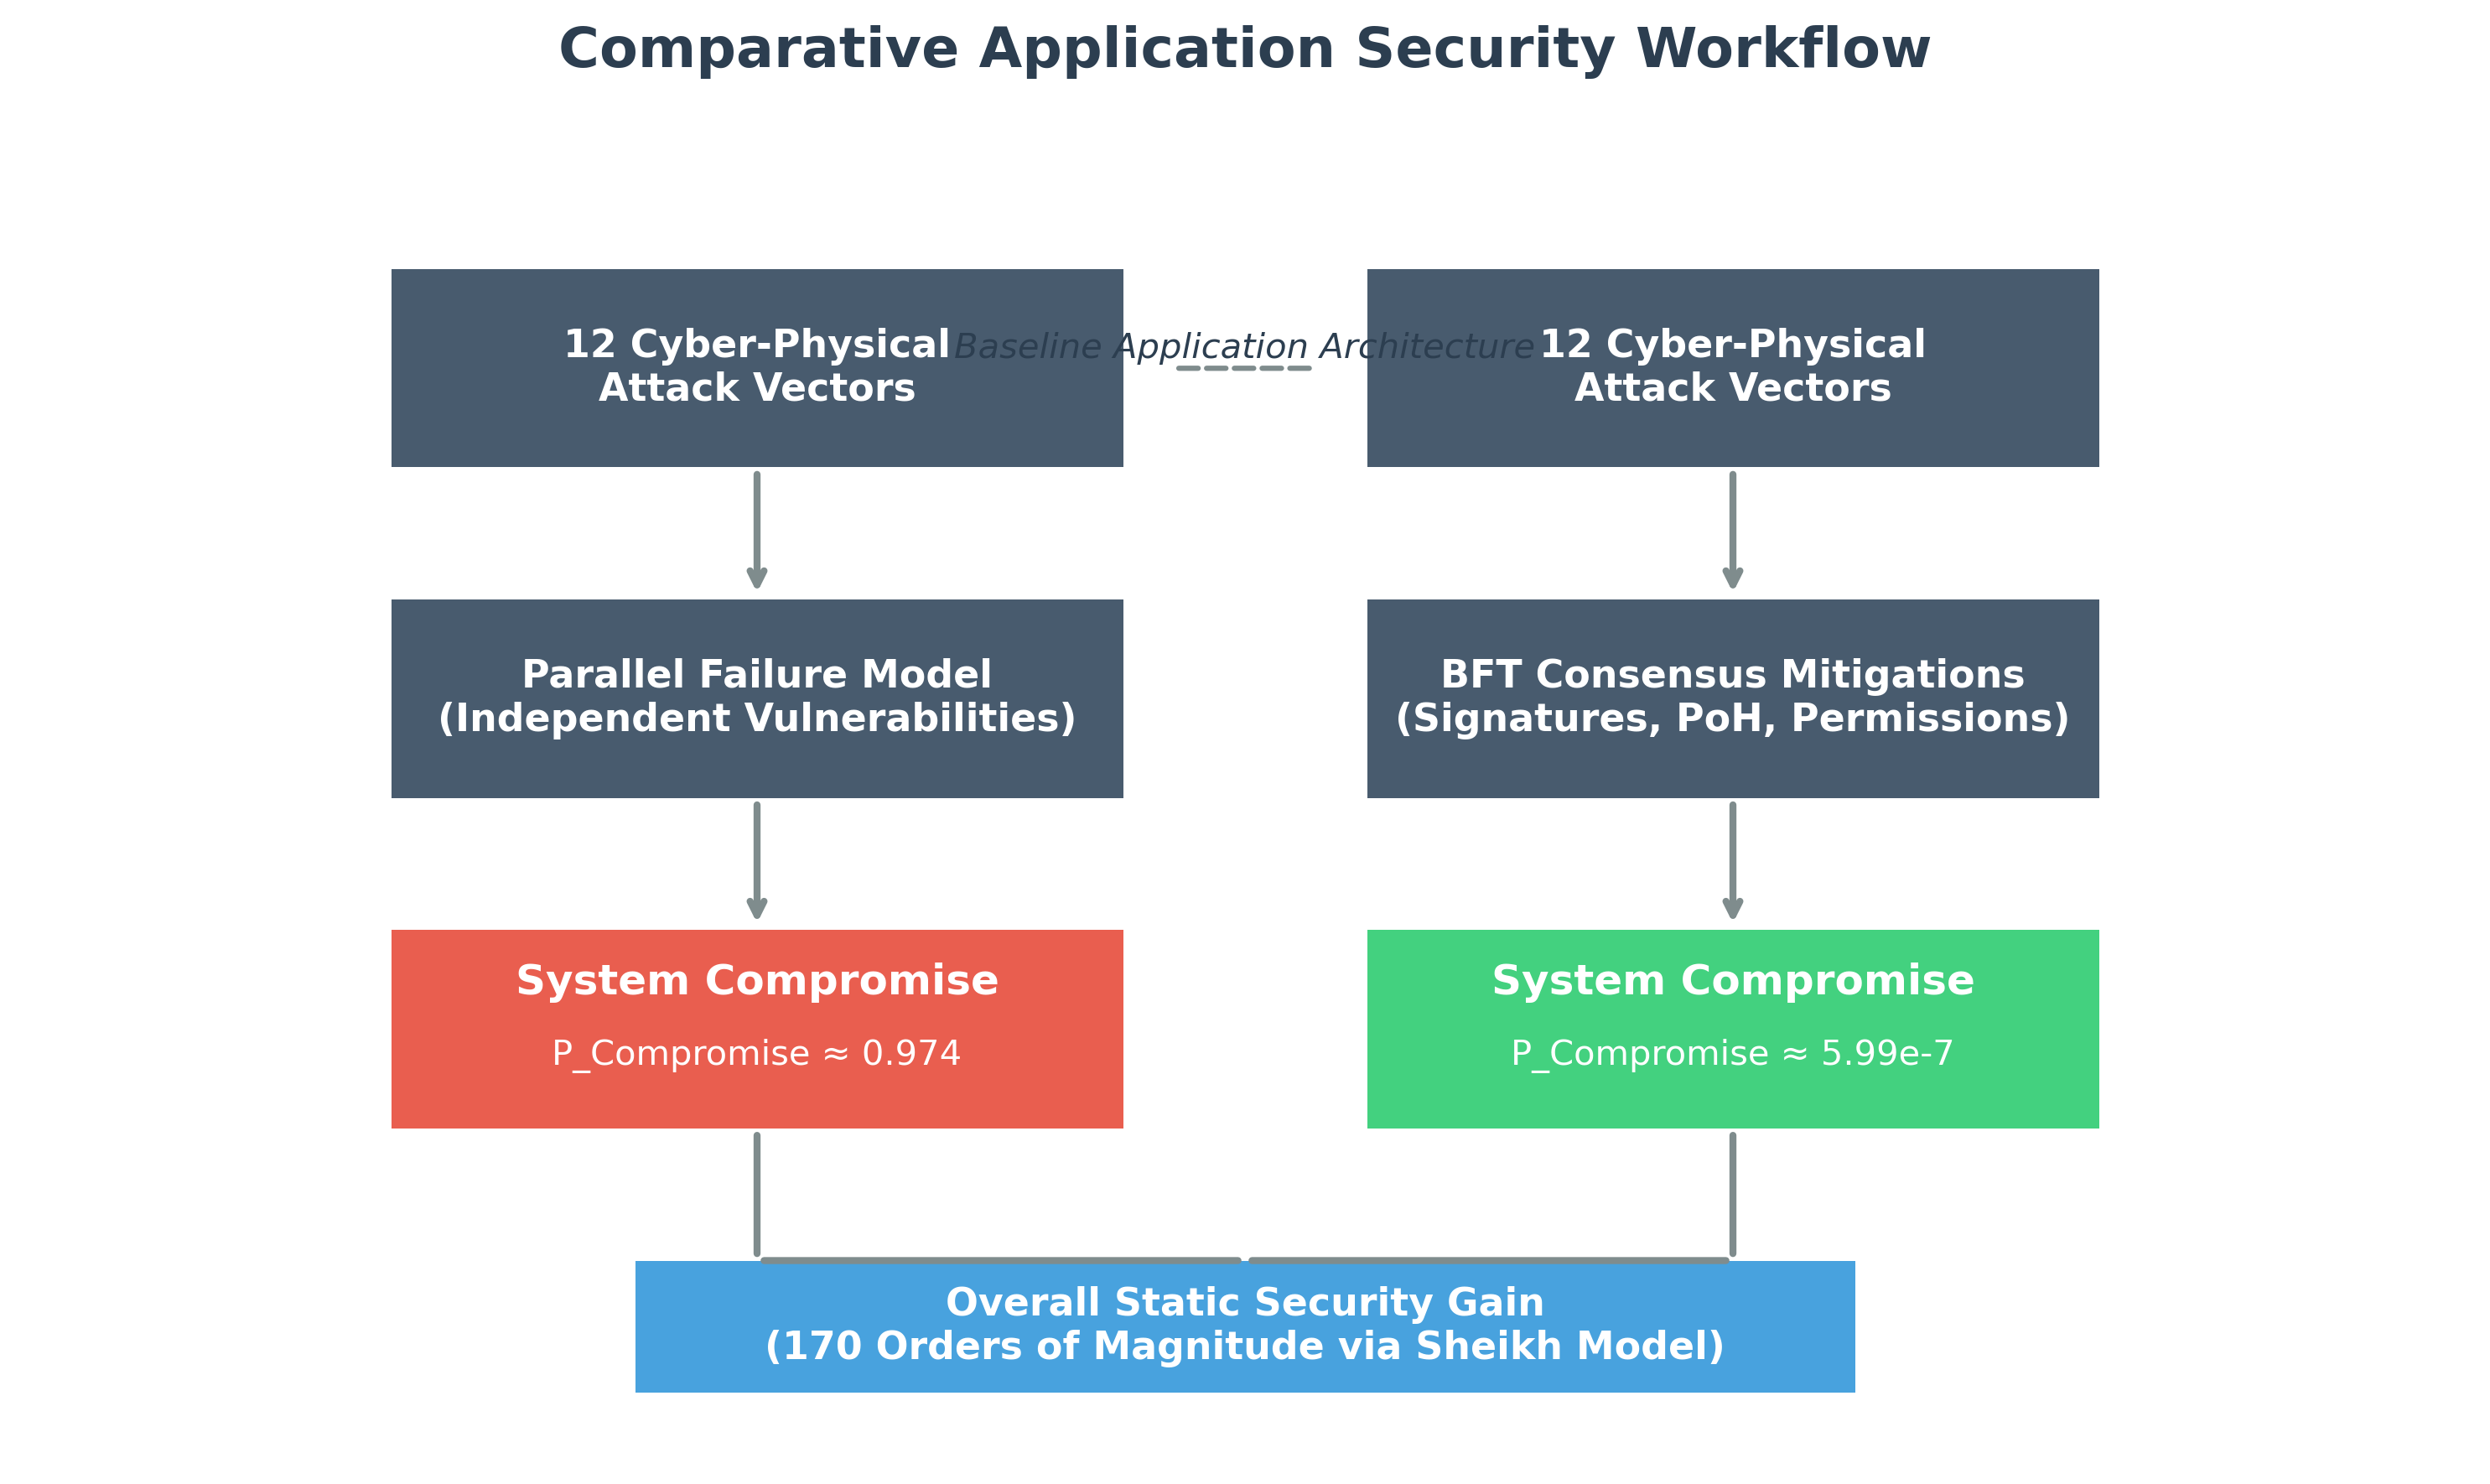
\includegraphics[width=0.75\textwidth]{figures/fig_comparative_workflow.png}
\end{figure}
\clearpage

\section{Component Contribution}
\textbf{File:} \texttt{fig\_component\_contribution.png} \\
\textbf{Concept/Origin:} This plot visualizes \textbf{Component Contribution Metric} as a function of \textbf{Time / Baseline Parameter}. \\
\textbf{Equations/Framework:} 
Empirical baseline calculation from simulation data.
\vspace{0.5cm}
\begin{figure}[H]
    \centering
    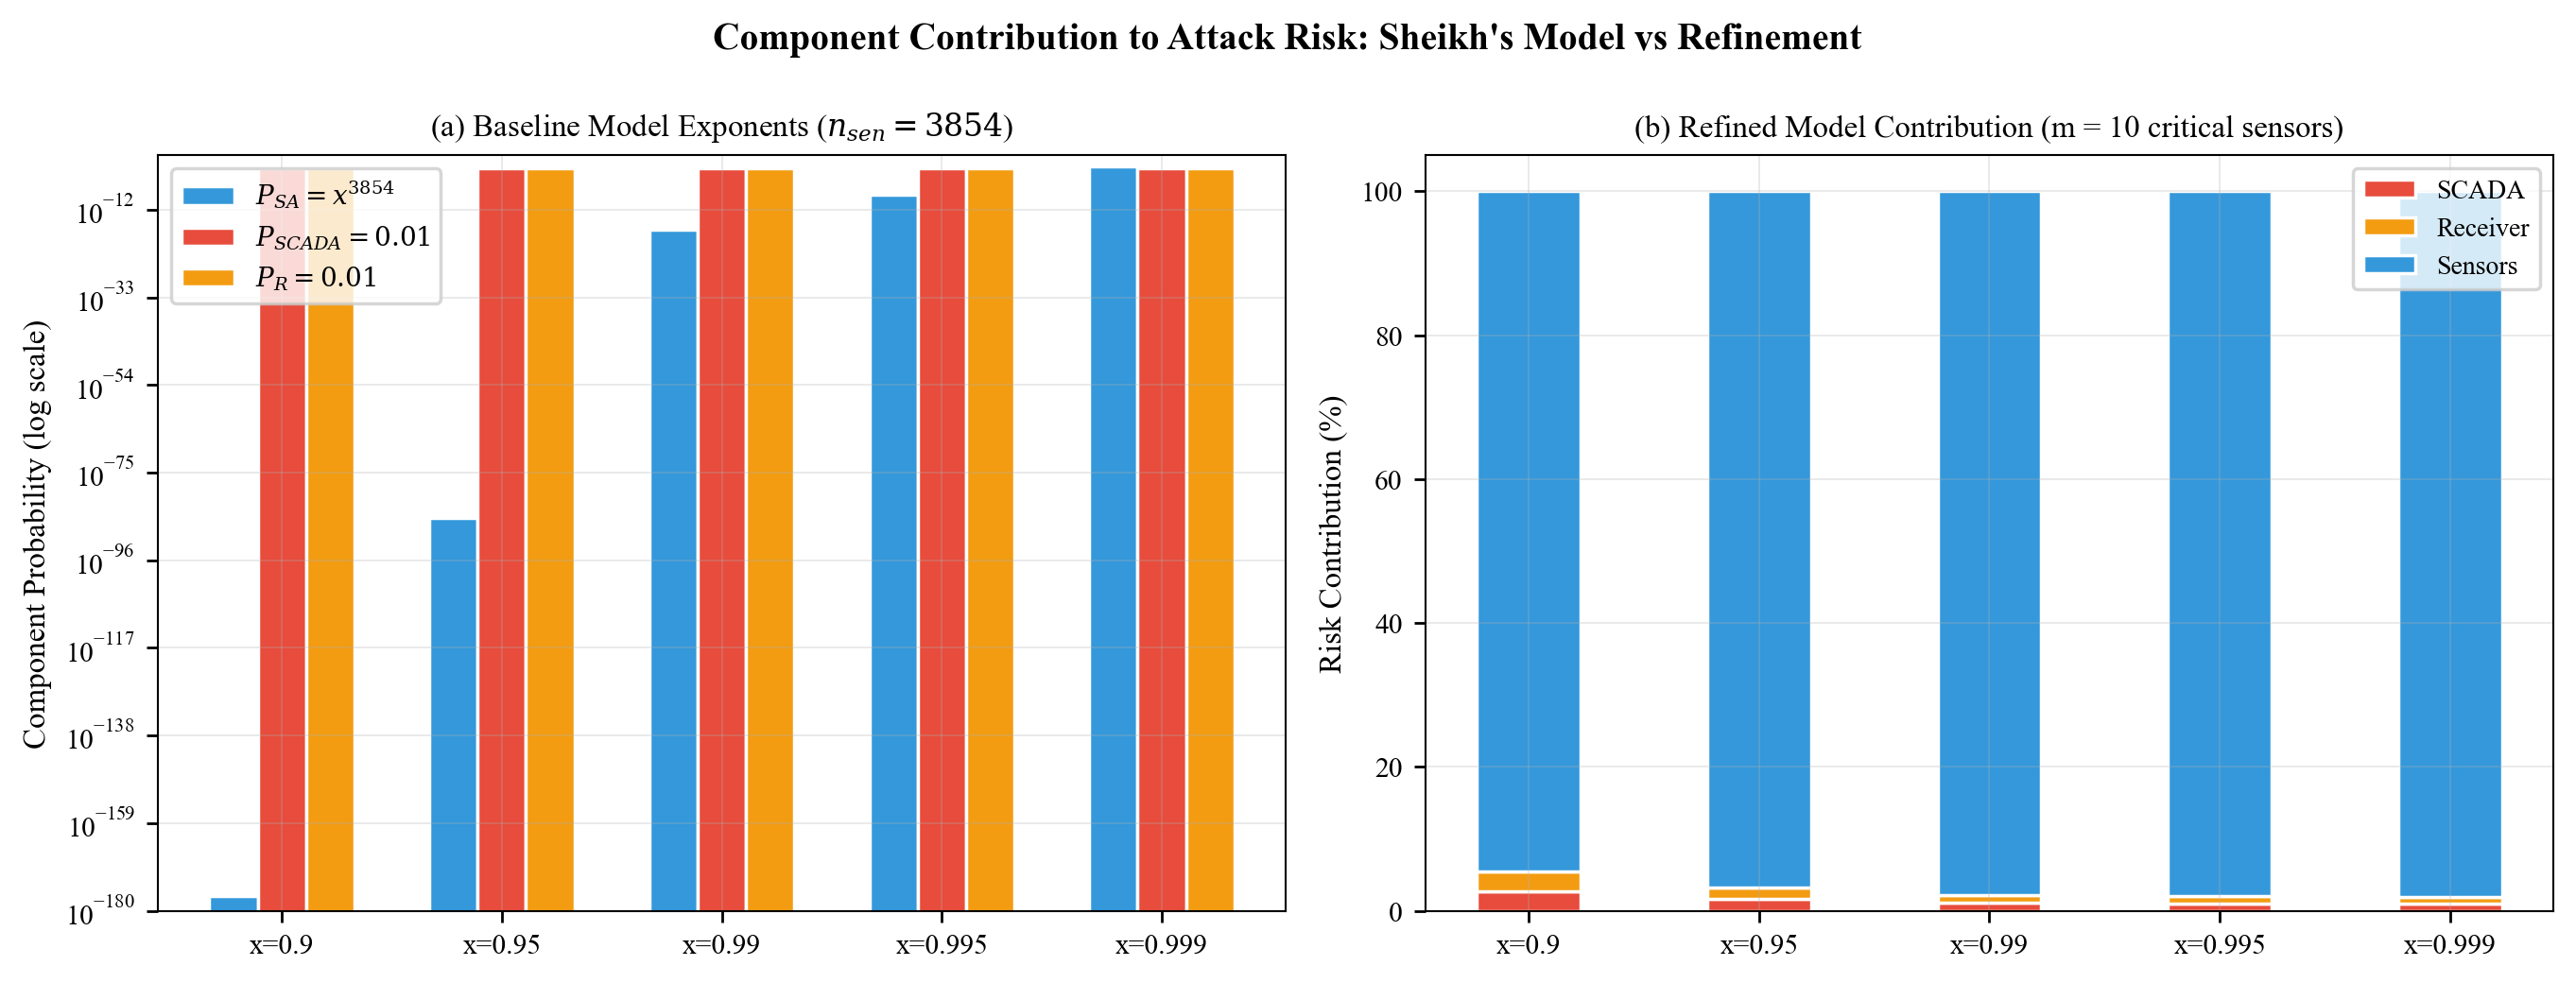
\includegraphics[width=0.75\textwidth]{figures/fig_component_contribution.png}
\end{figure}
\clearpage

\section{Correlation Sensitivity}
\textbf{File:} \texttt{fig\_correlation\_sensitivity.png} \\
\textbf{Concept/Origin:} This plot visualizes \textbf{Correlation Sensitivity Metric} as a function of \textbf{Time / Baseline Parameter}. \\
\textbf{Equations/Framework:} 
Empirical baseline calculation from simulation data.
\vspace{0.5cm}
\begin{figure}[H]
    \centering
    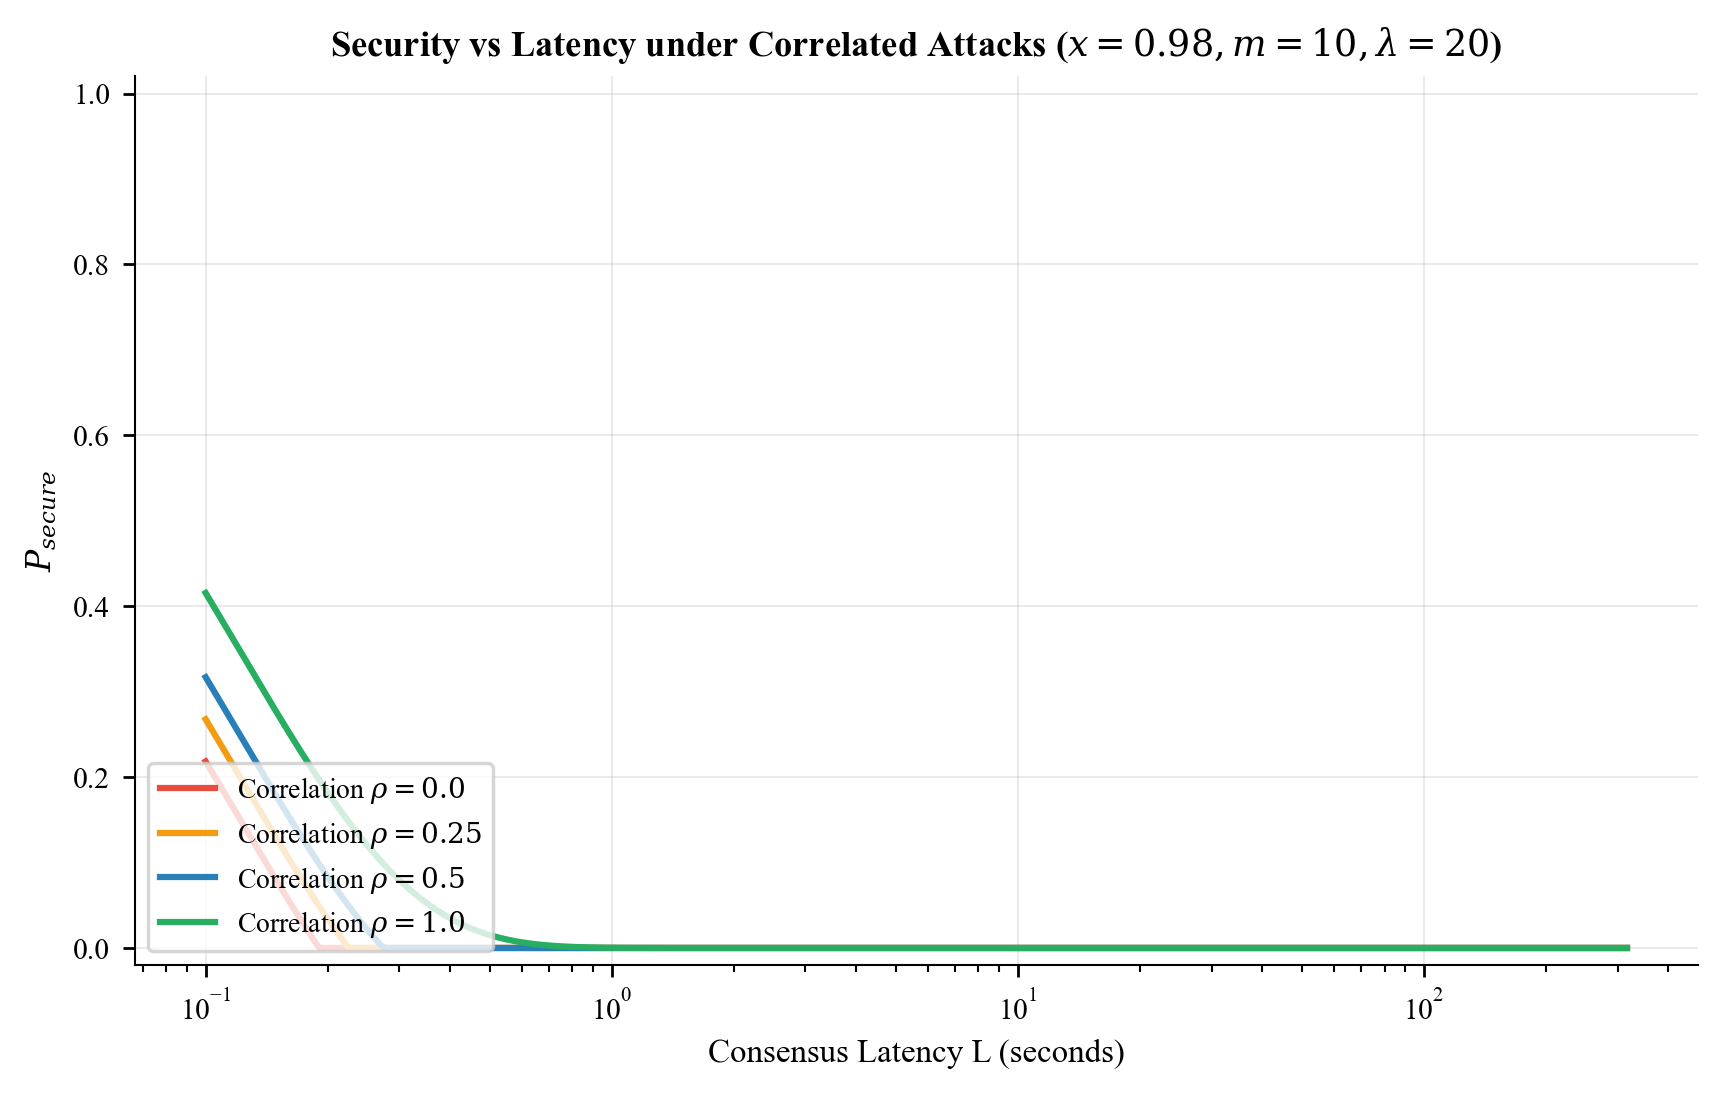
\includegraphics[width=0.75\textwidth]{figures/fig_correlation_sensitivity.png}
\end{figure}
\clearpage

\section{Eta Sensitivity}
\textbf{File:} \texttt{fig\_eta\_sensitivity.png} \\
\textbf{Concept/Origin:} This plot visualizes \textbf{Eta Sensitivity Metric} as a function of \textbf{Time / Baseline Parameter}. \\
\textbf{Equations/Framework:} 
Empirical baseline calculation from simulation data.
\vspace{0.5cm}
\begin{figure}[H]
    \centering
    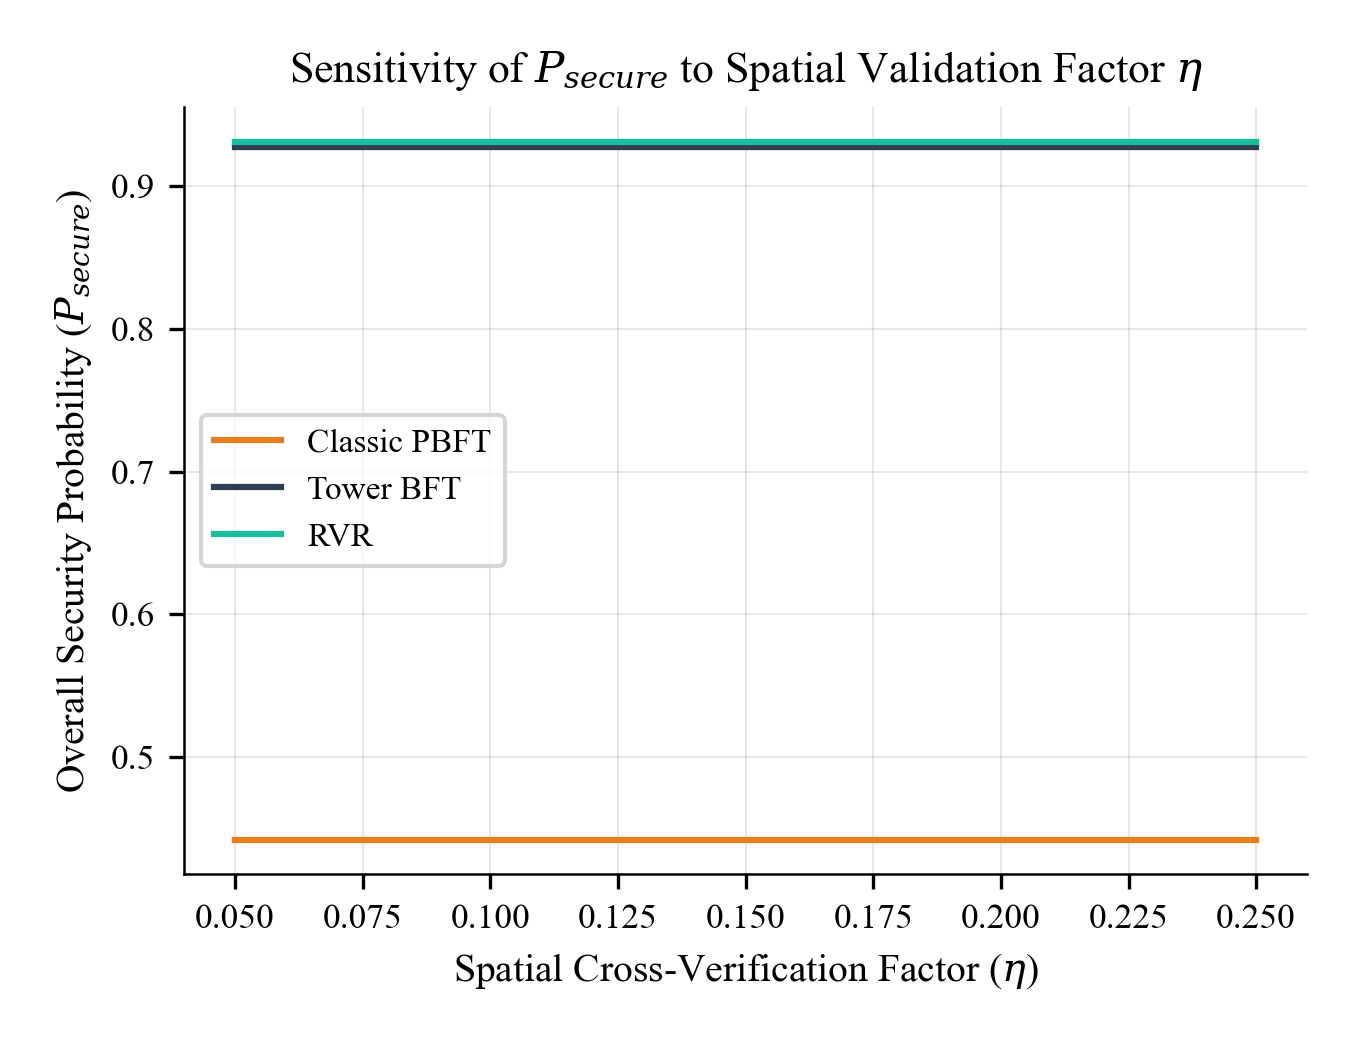
\includegraphics[width=0.75\textwidth]{figures/fig_eta_sensitivity.png}
\end{figure}
\clearpage

\section{F Vs Latency}
\textbf{File:} \texttt{fig\_f\_vs\_latency.png} \\
\textbf{Concept/Origin:} This plot visualizes \textbf{F} as a function of \textbf{Latency}. \\
\textbf{Equations/Framework:} 
 L_{total} = L_{net} + L_{consensus} 
\vspace{0.5cm}
\begin{figure}[H]
    \centering
    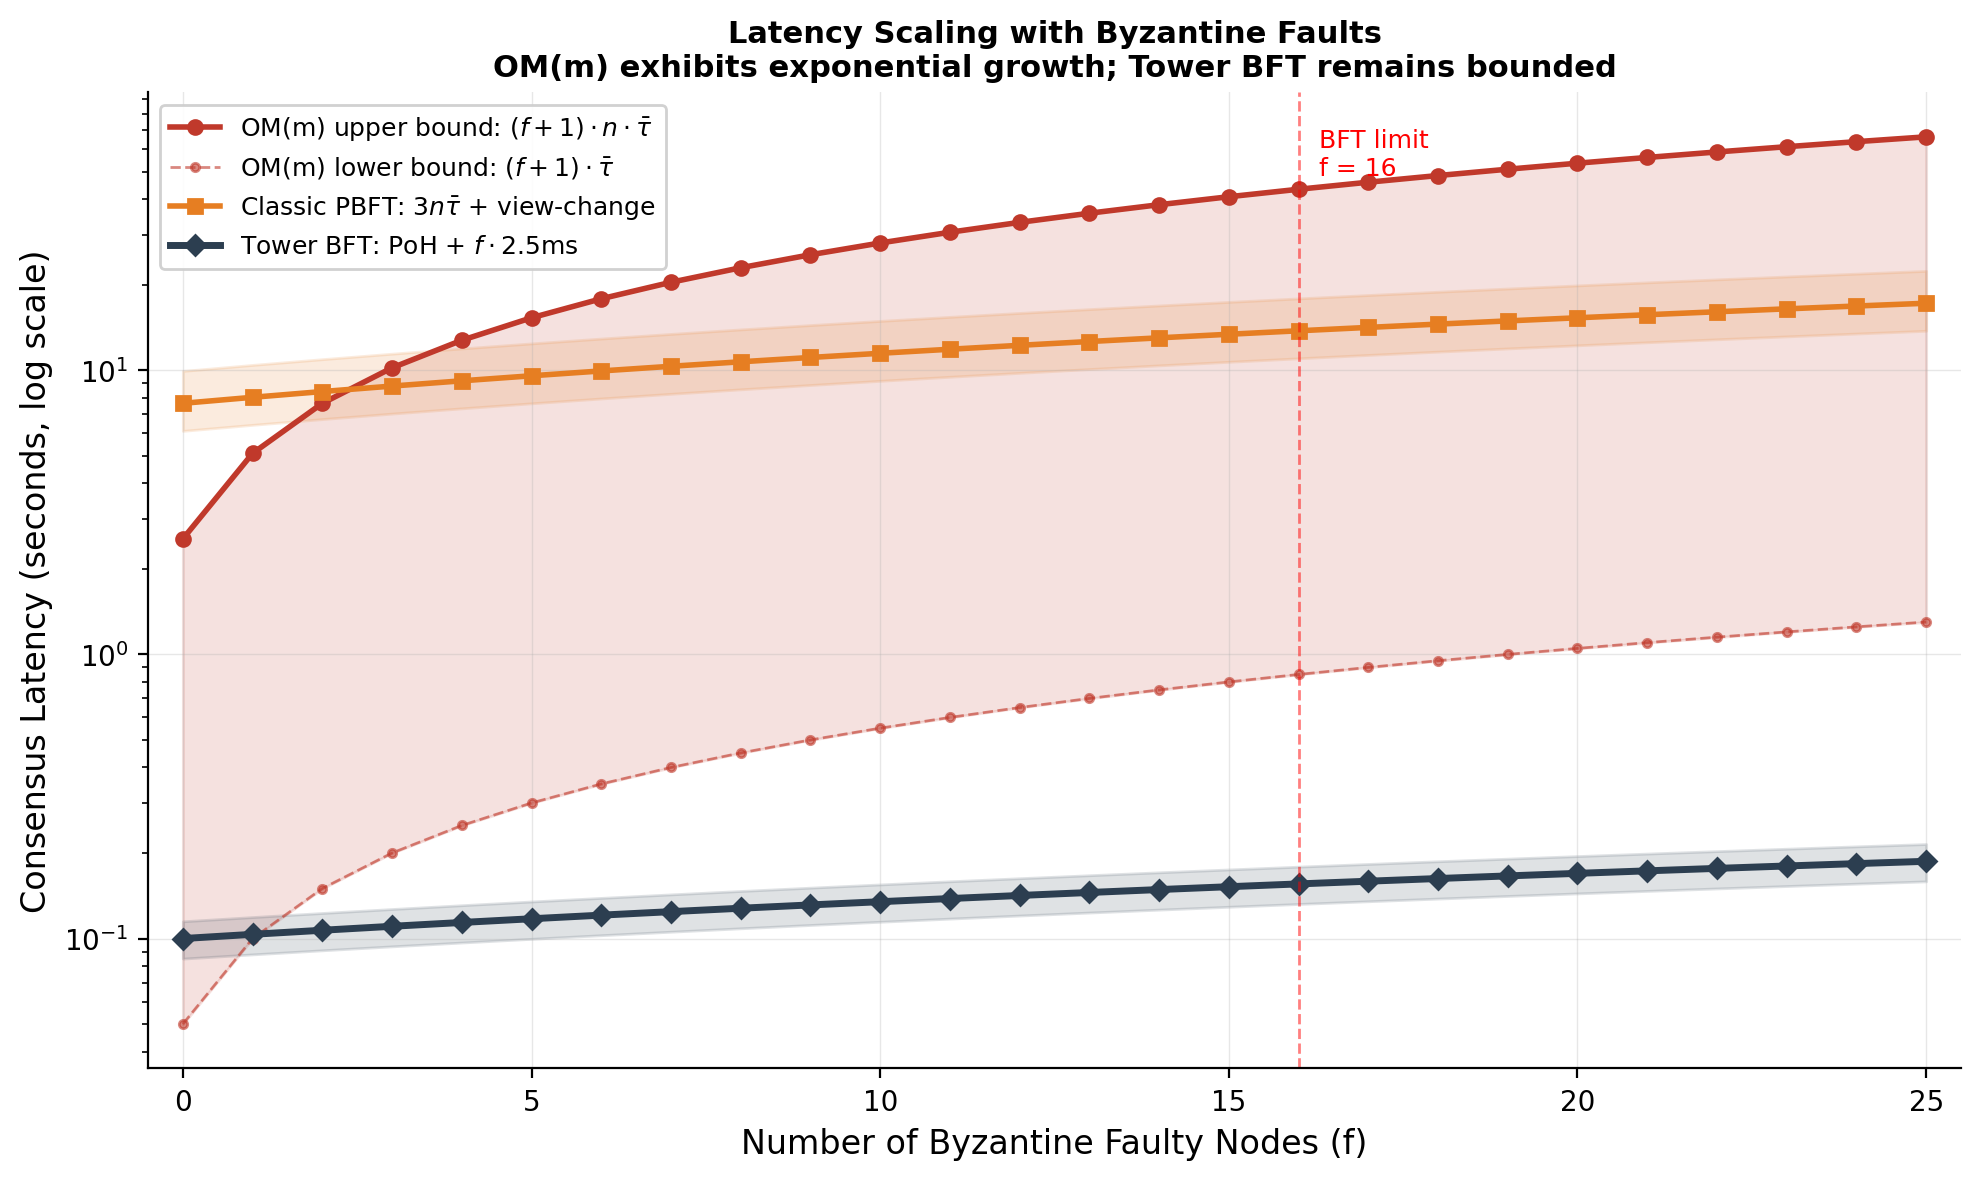
\includegraphics[width=0.75\textwidth]{figures/fig_f_vs_latency.png}
\end{figure}
\clearpage

\section{F Vs Psecure}
\textbf{File:} \texttt{fig\_f\_vs\_psecure.png} \\
\textbf{Concept/Origin:} This plot visualizes \textbf{F} as a function of \textbf{Psecure}. \\
\textbf{Equations/Framework:} 
 P_{Byz} = \sum_{i=f+1}^{n} \binom{n}{i} p_c^i (1-p_c)^{n-i} 
 P_{temporal} = 1 - e^{-\lambda L P_{TA}} 
\vspace{0.5cm}
\begin{figure}[H]
    \centering
    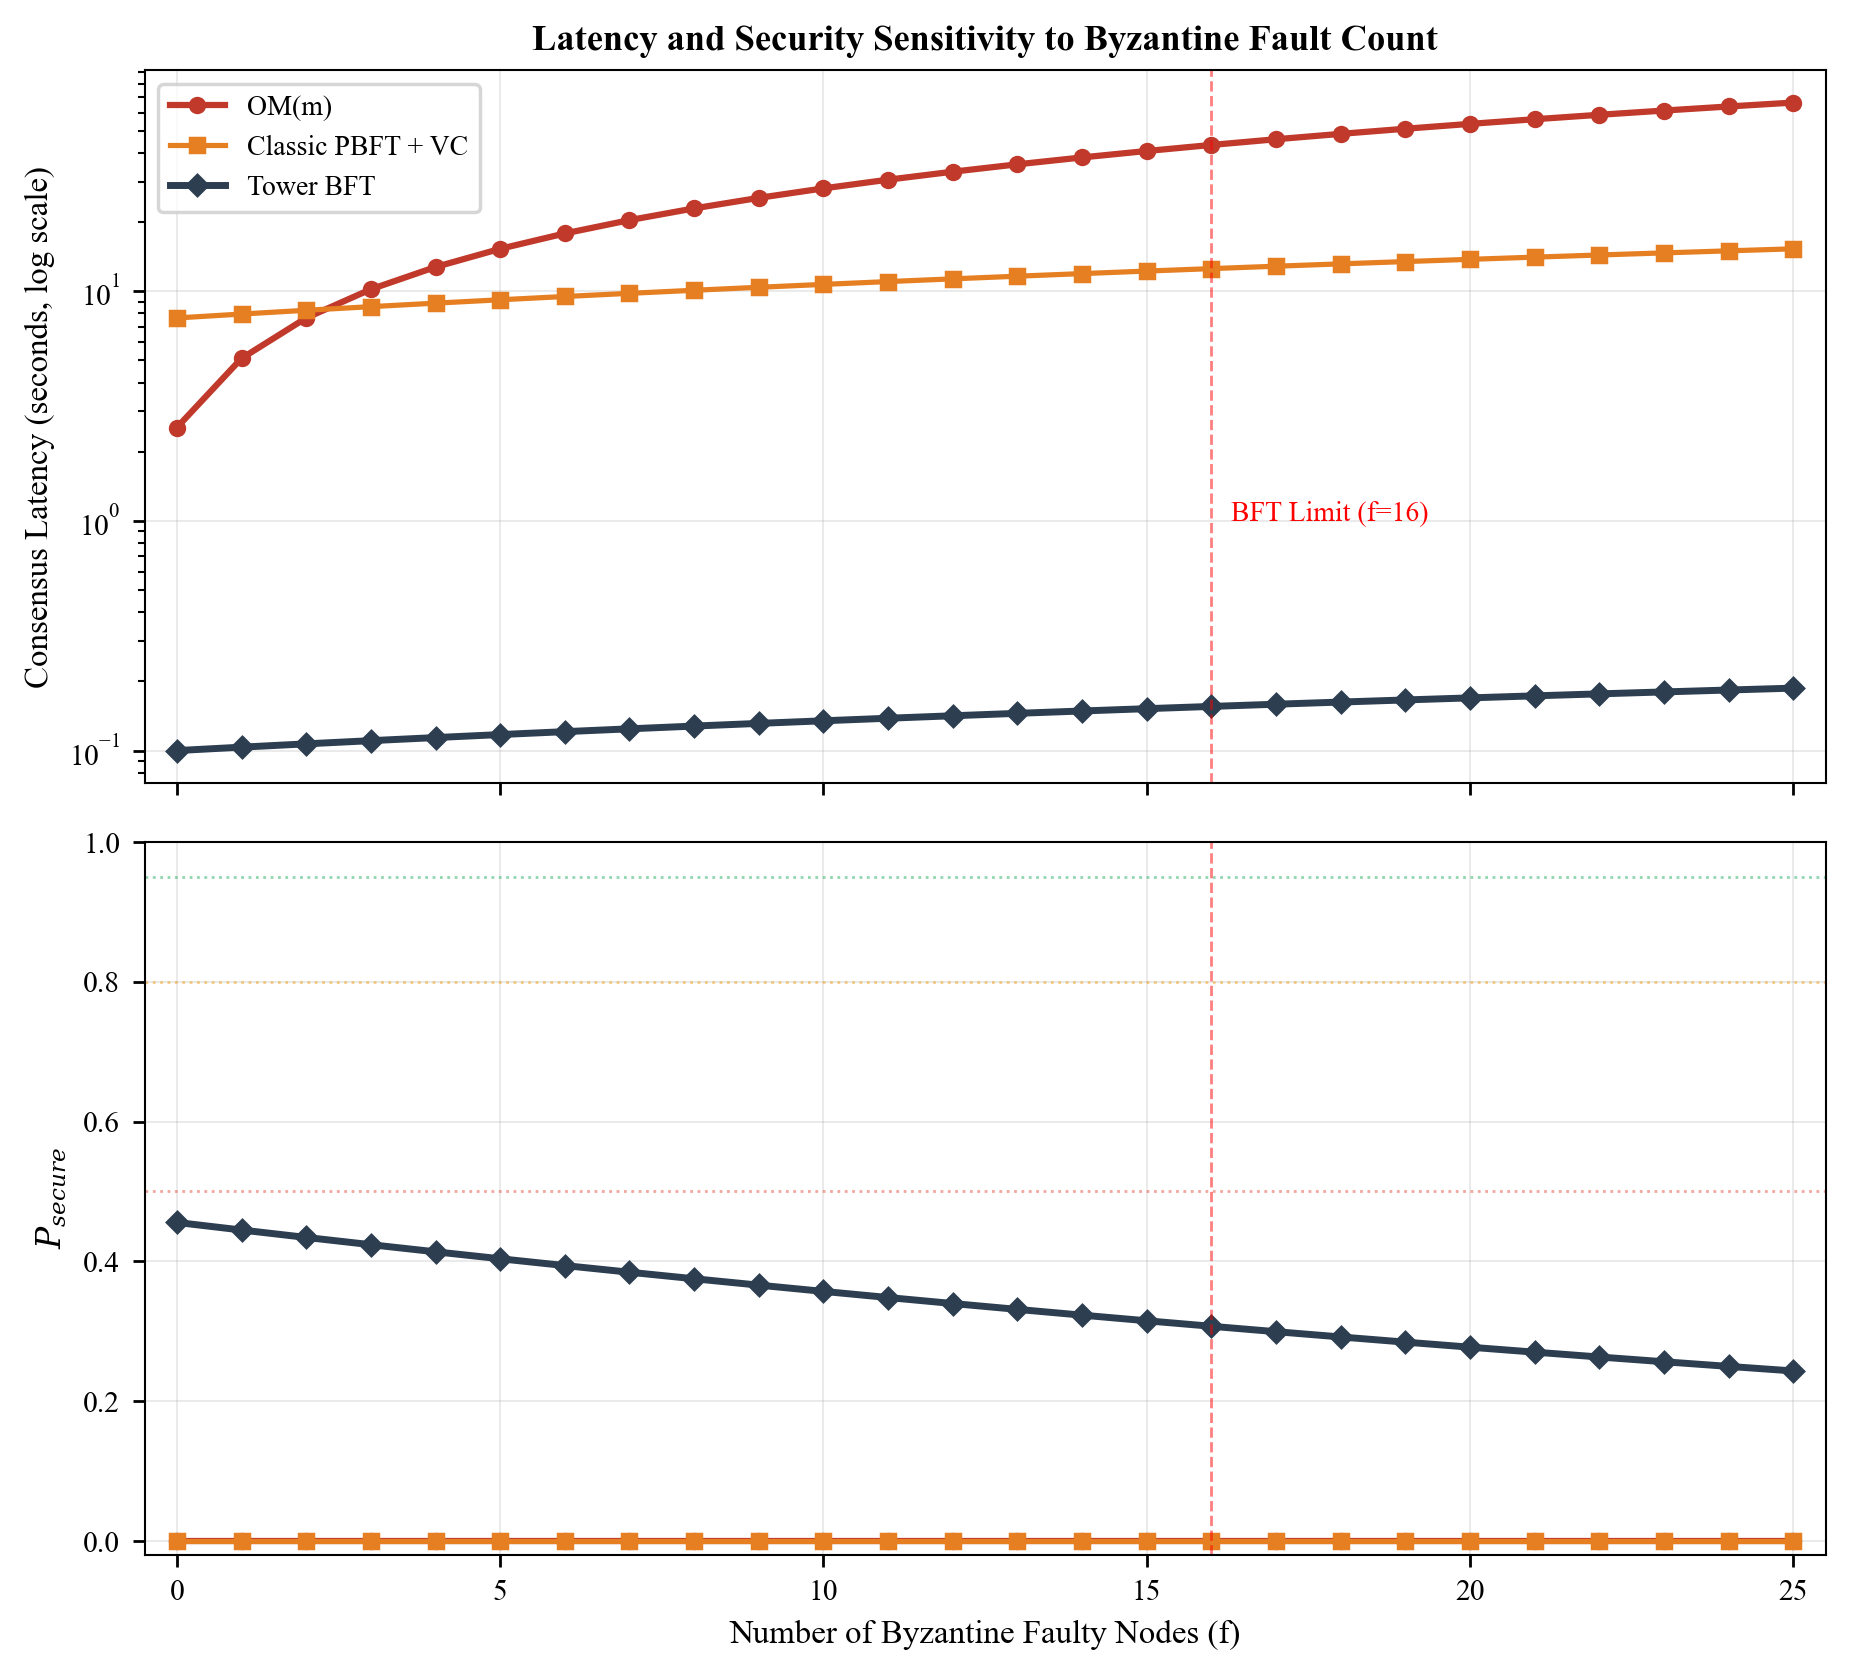
\includegraphics[width=0.75\textwidth]{figures/fig_f_vs_psecure.png}
\end{figure}
\clearpage

\section{Key Management}
\textbf{File:} \texttt{fig\_key\_management.png} \\
\textbf{Concept/Origin:} This plot visualizes \textbf{Key Management Metric} as a function of \textbf{Time / Baseline Parameter}. \\
\textbf{Equations/Framework:} 
Empirical baseline calculation from simulation data.
\vspace{0.5cm}
\begin{figure}[H]
    \centering
    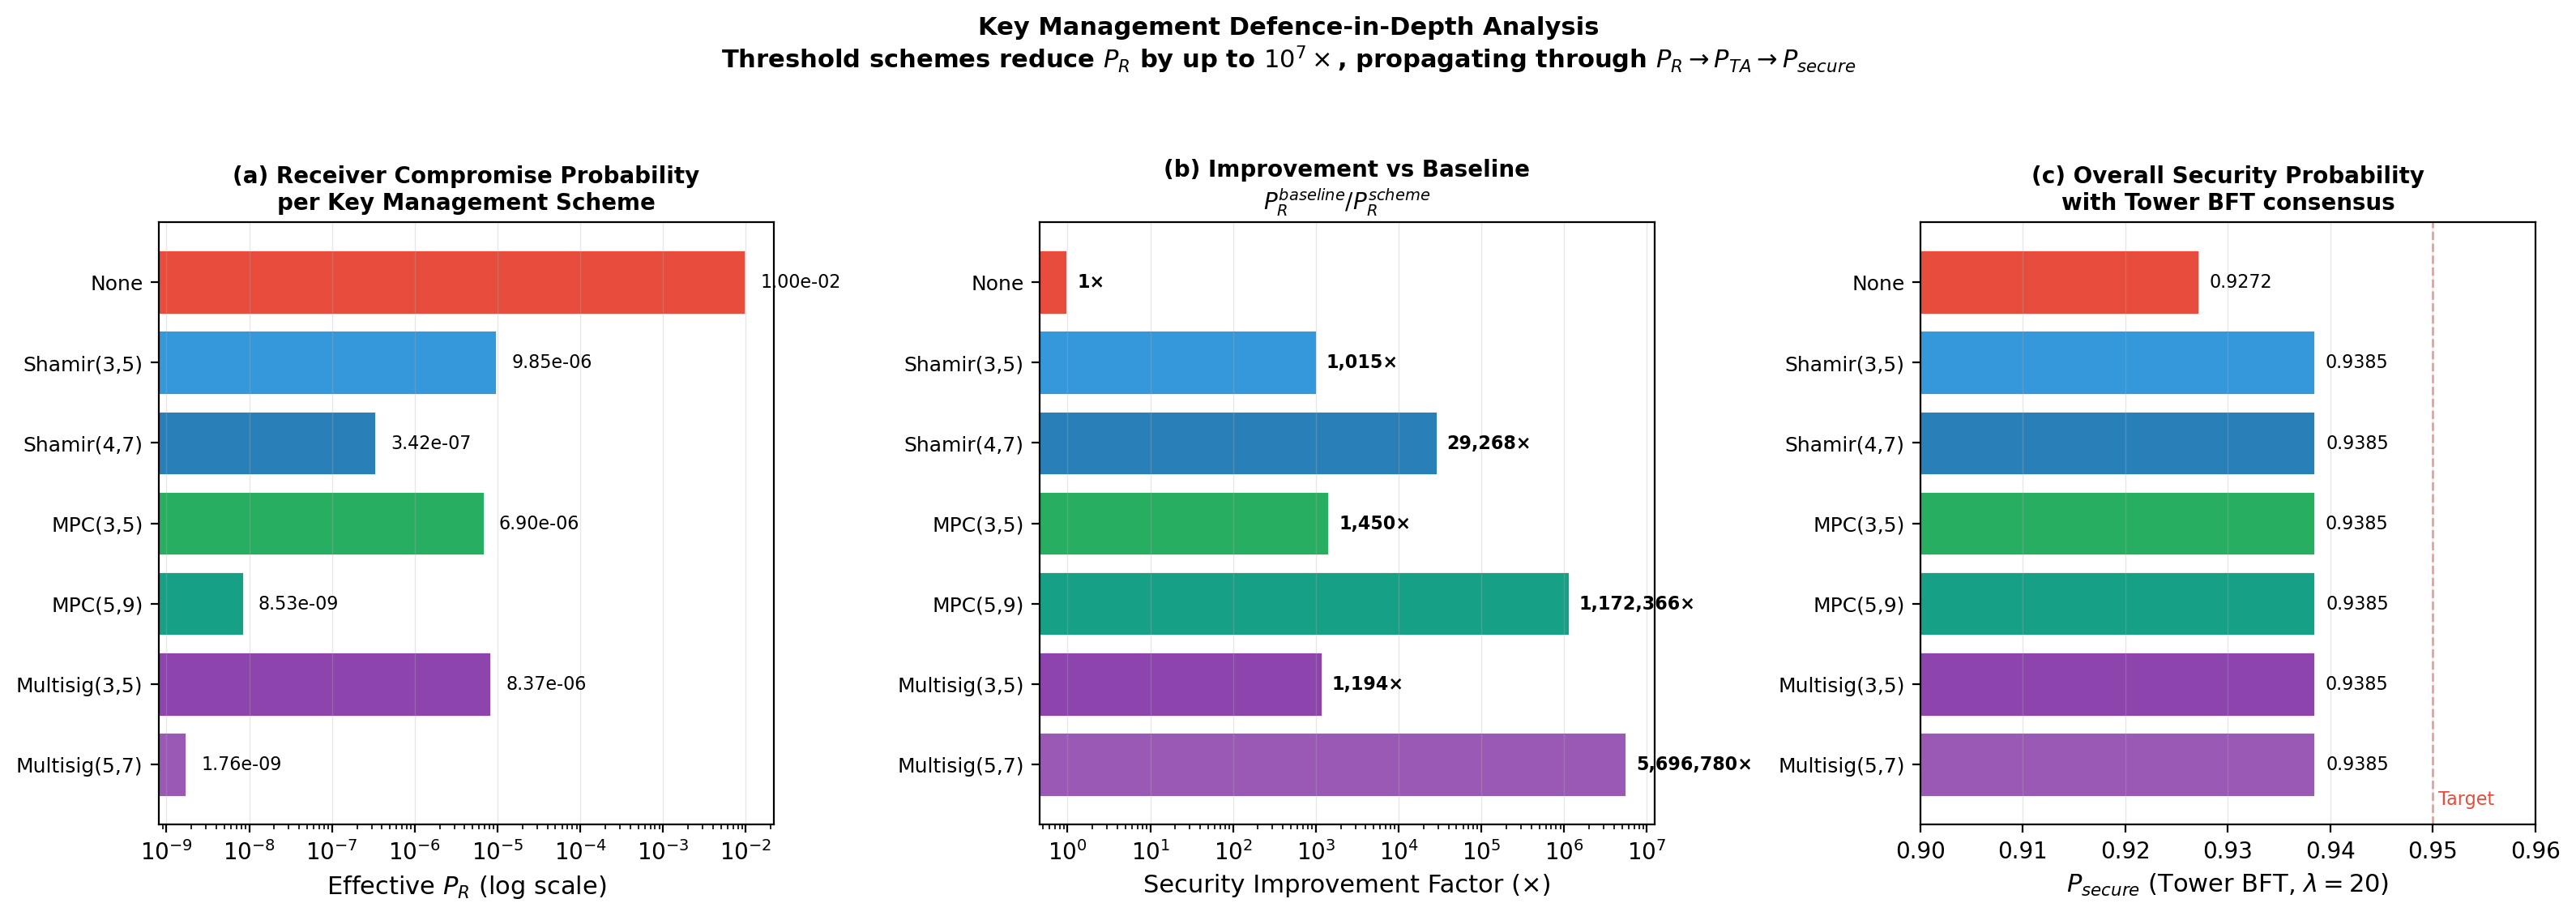
\includegraphics[width=0.75\textwidth]{figures/fig_key_management.png}
\end{figure}
\clearpage

\section{Latency Distribution}
\textbf{File:} \texttt{fig\_latency\_distribution.png} \\
\textbf{Concept/Origin:} This plot visualizes \textbf{Latency Distribution Metric} as a function of \textbf{Time / Baseline Parameter}. \\
\textbf{Equations/Framework:} 
 L_{total} = L_{net} + L_{consensus} 
\vspace{0.5cm}
\begin{figure}[H]
    \centering
    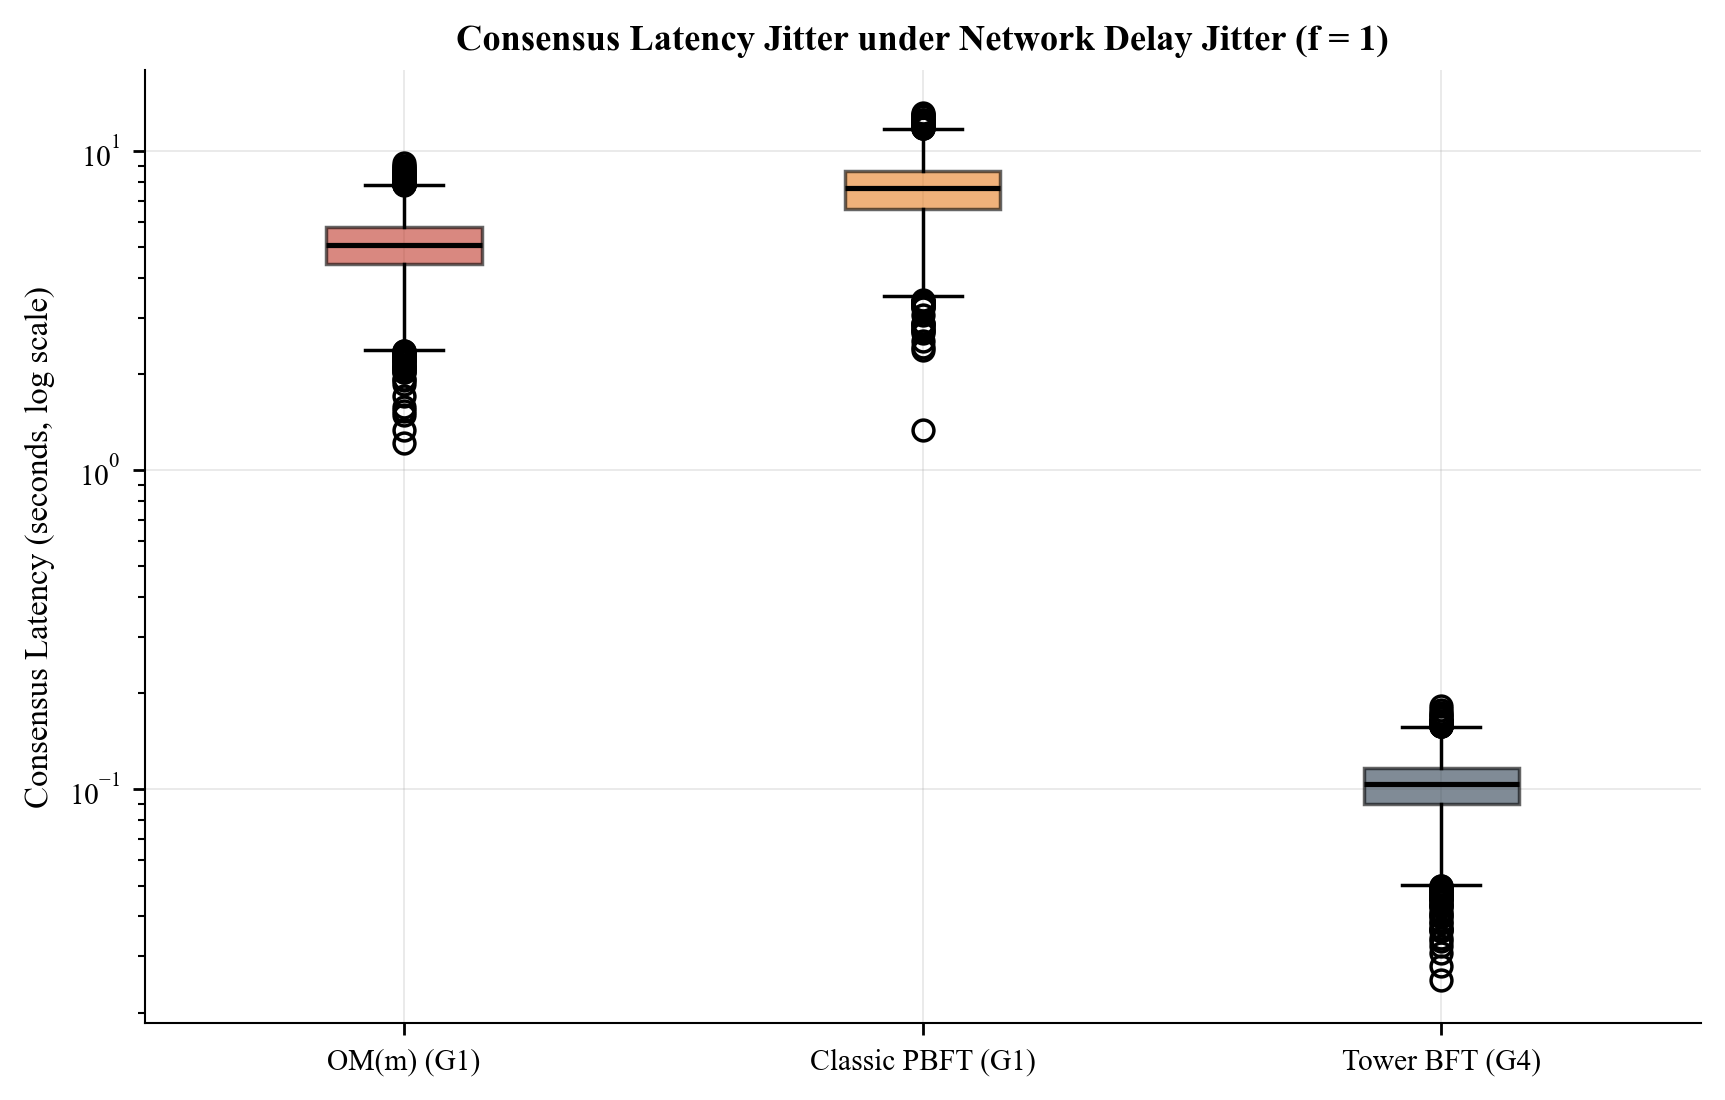
\includegraphics[width=0.75\textwidth]{figures/fig_latency_distribution.png}
\end{figure}
\clearpage

\section{Latency Vs Psecure}
\textbf{File:} \texttt{fig\_latency\_vs\_psecure.png} \\
\textbf{Concept/Origin:} This plot visualizes \textbf{Latency} as a function of \textbf{Psecure}. \\
\textbf{Equations/Framework:} 
 L_{total} = L_{net} + L_{consensus} 
\vspace{0.5cm}
\begin{figure}[H]
    \centering
    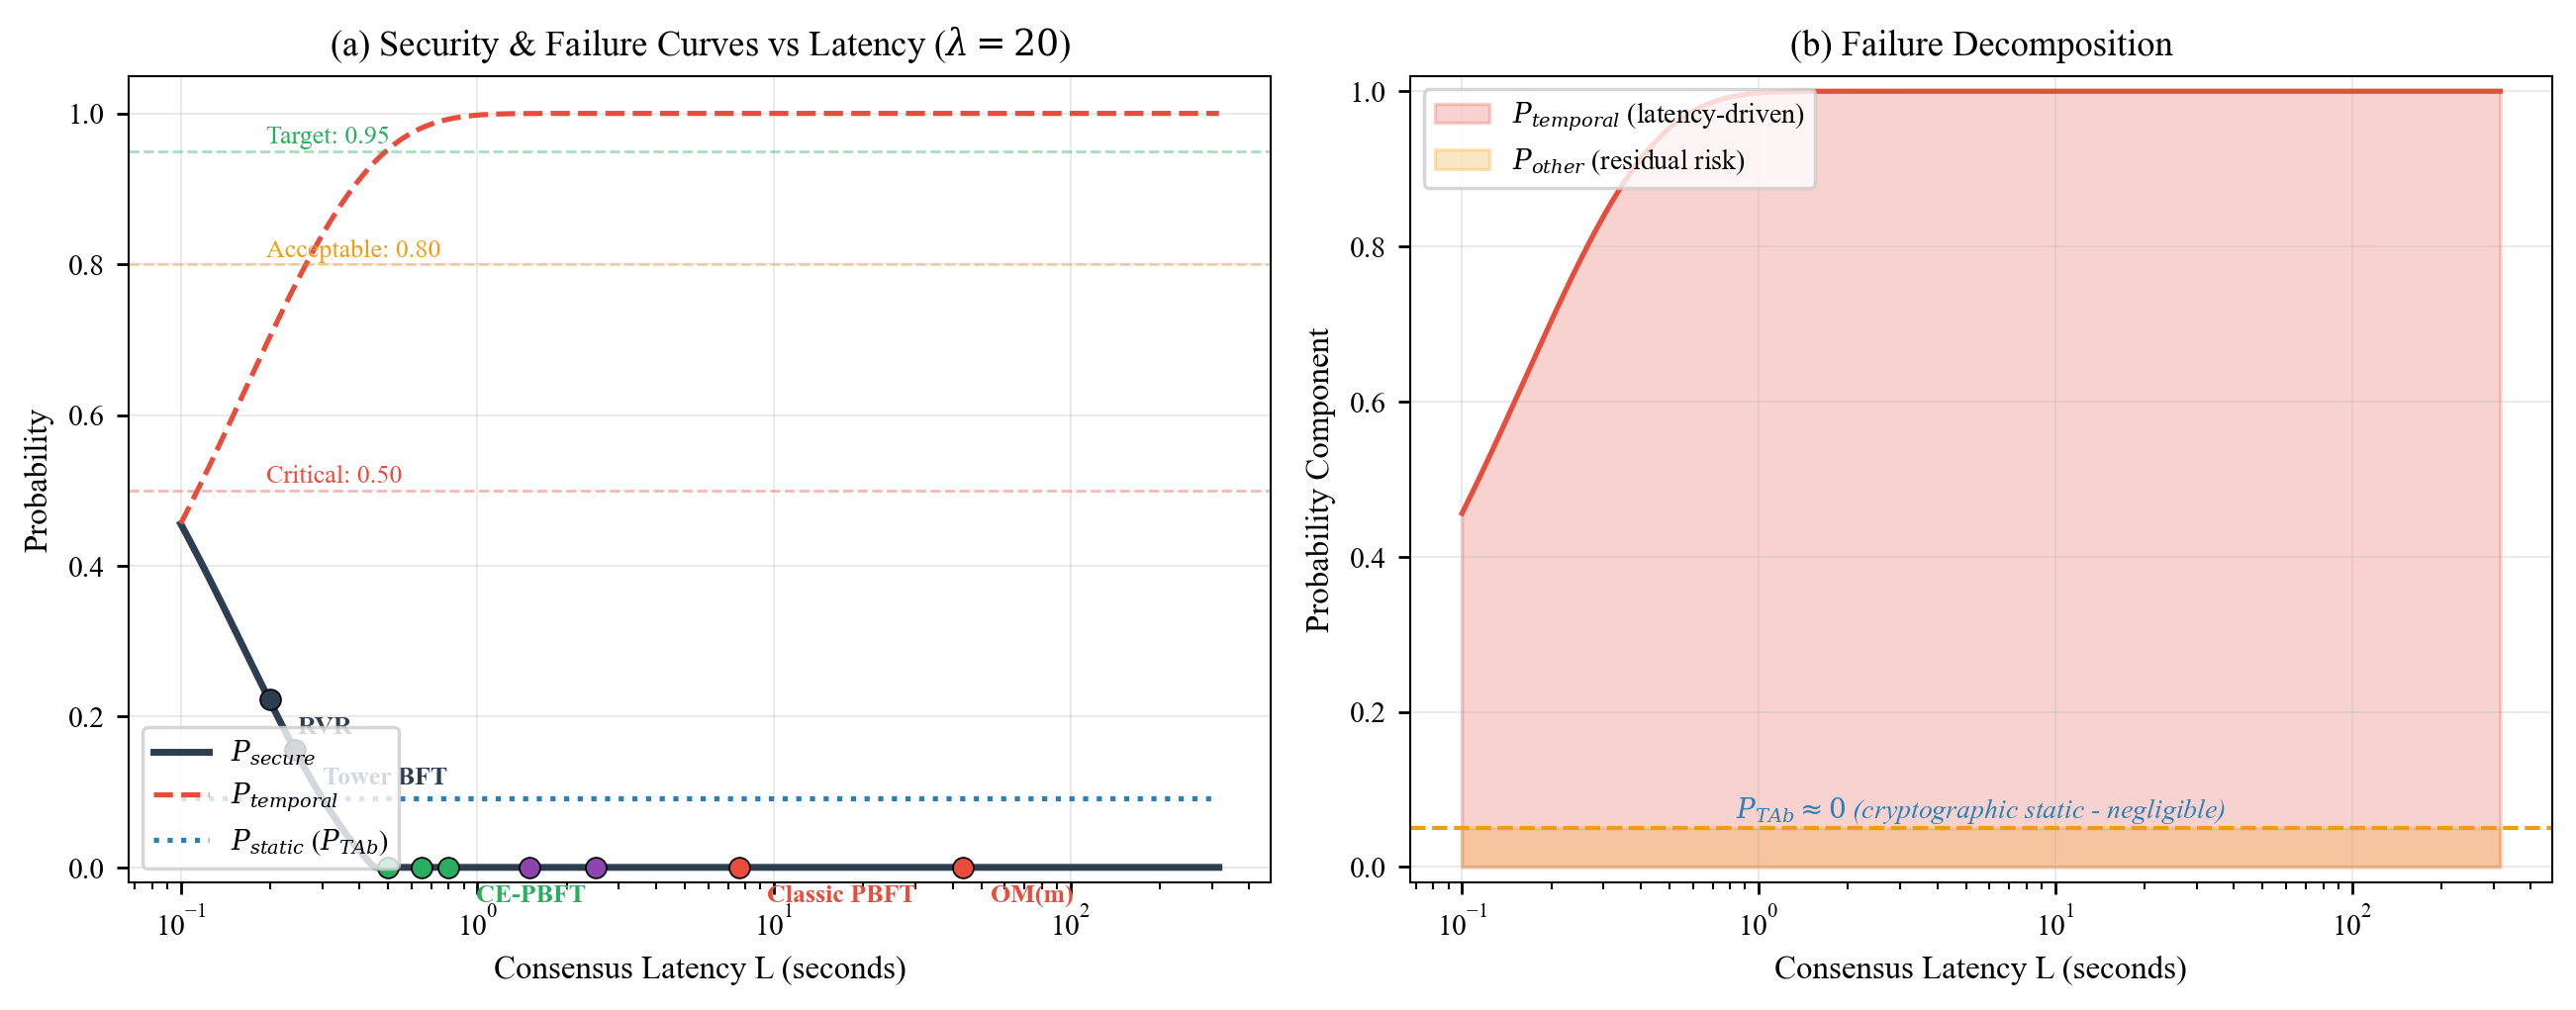
\includegraphics[width=0.75\textwidth]{figures/fig_latency_vs_psecure.png}
\end{figure}
\clearpage

\section{Message Complexity}
\textbf{File:} \texttt{fig\_message\_complexity.png} \\
\textbf{Concept/Origin:} This plot visualizes \textbf{Message Complexity Metric} as a function of \textbf{Time / Baseline Parameter}. \\
\textbf{Equations/Framework:} 
 E_{total} = E_{tx} + E_{rx} + E_{crypto} 
\vspace{0.5cm}
\begin{figure}[H]
    \centering
    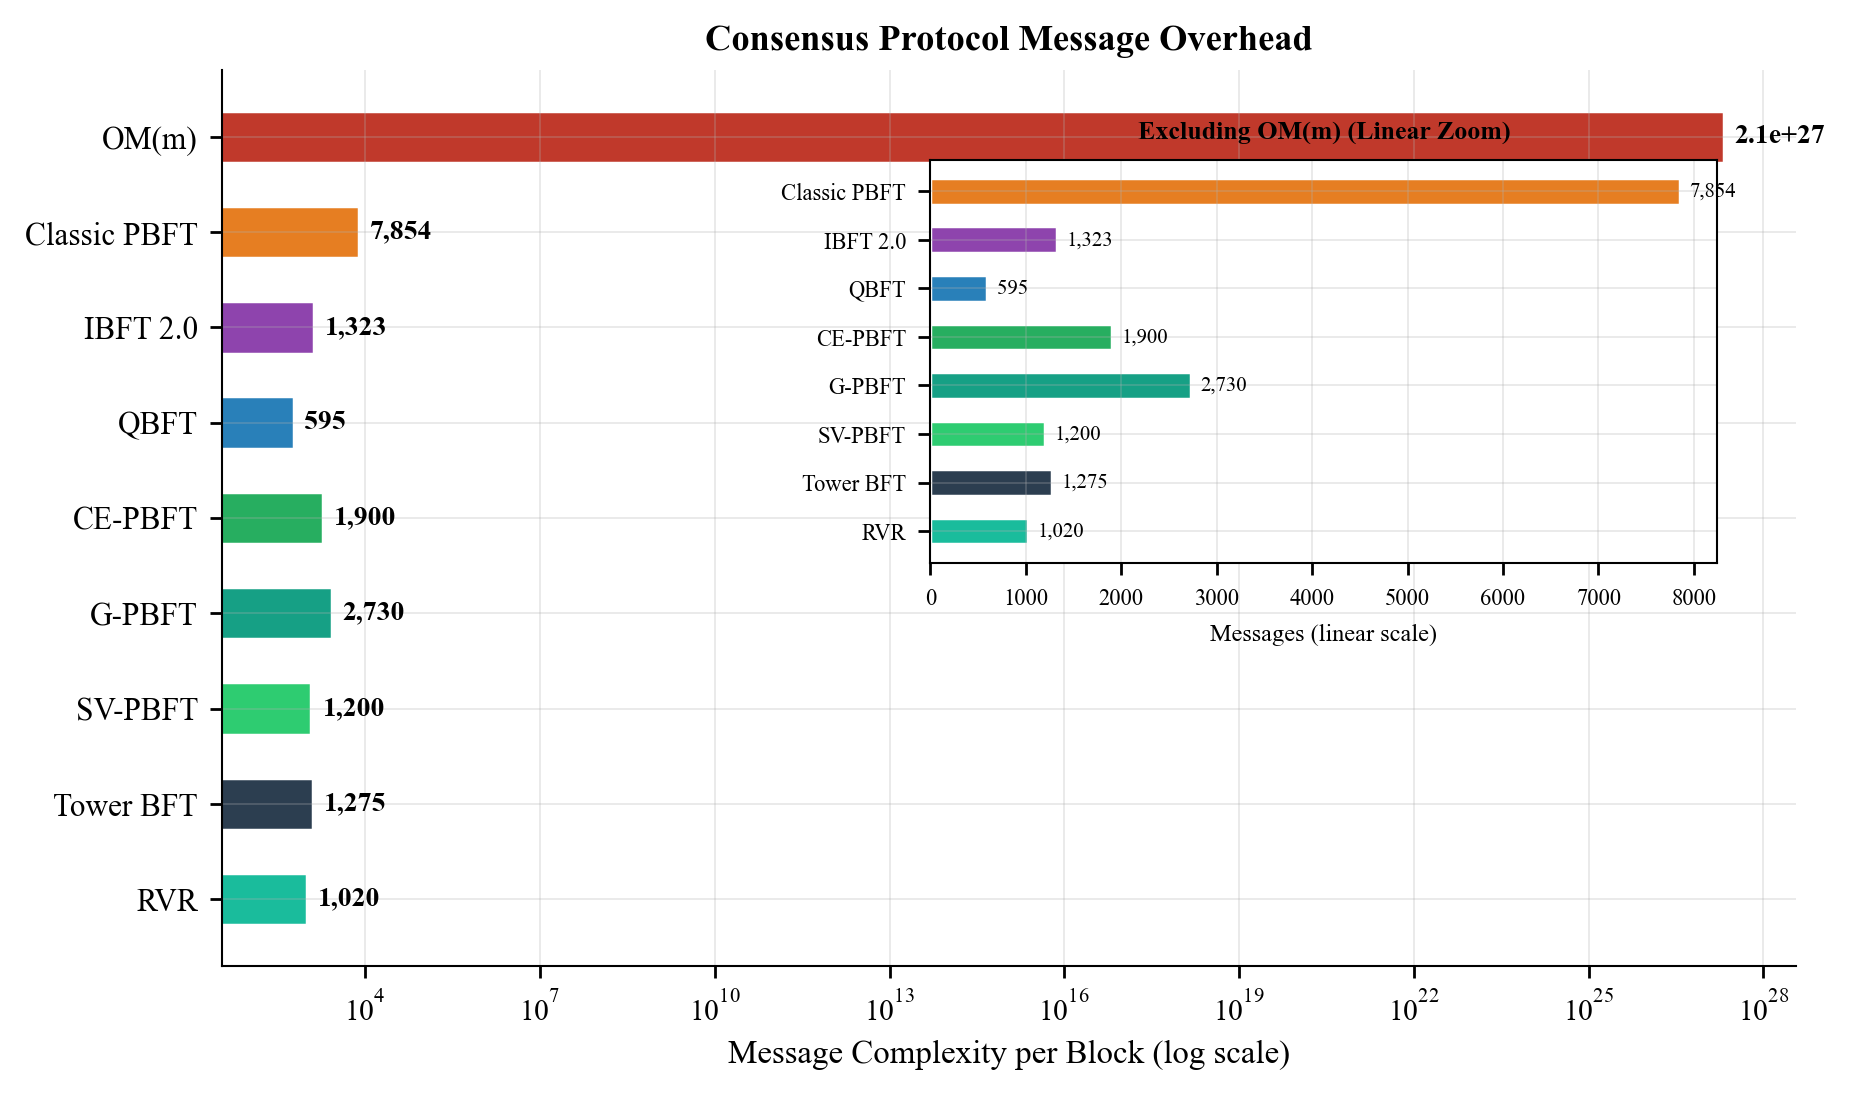
\includegraphics[width=0.75\textwidth]{figures/fig_message_complexity.png}
\end{figure}
\clearpage

\section{Model Comparison}
\textbf{File:} \texttt{fig\_model\_comparison.png} \\
\textbf{Concept/Origin:} This plot visualizes \textbf{Model Comparison Metric} as a function of \textbf{Time / Baseline Parameter}. \\
\textbf{Equations/Framework:} 
Empirical baseline calculation from simulation data.
\vspace{0.5cm}
\begin{figure}[H]
    \centering
    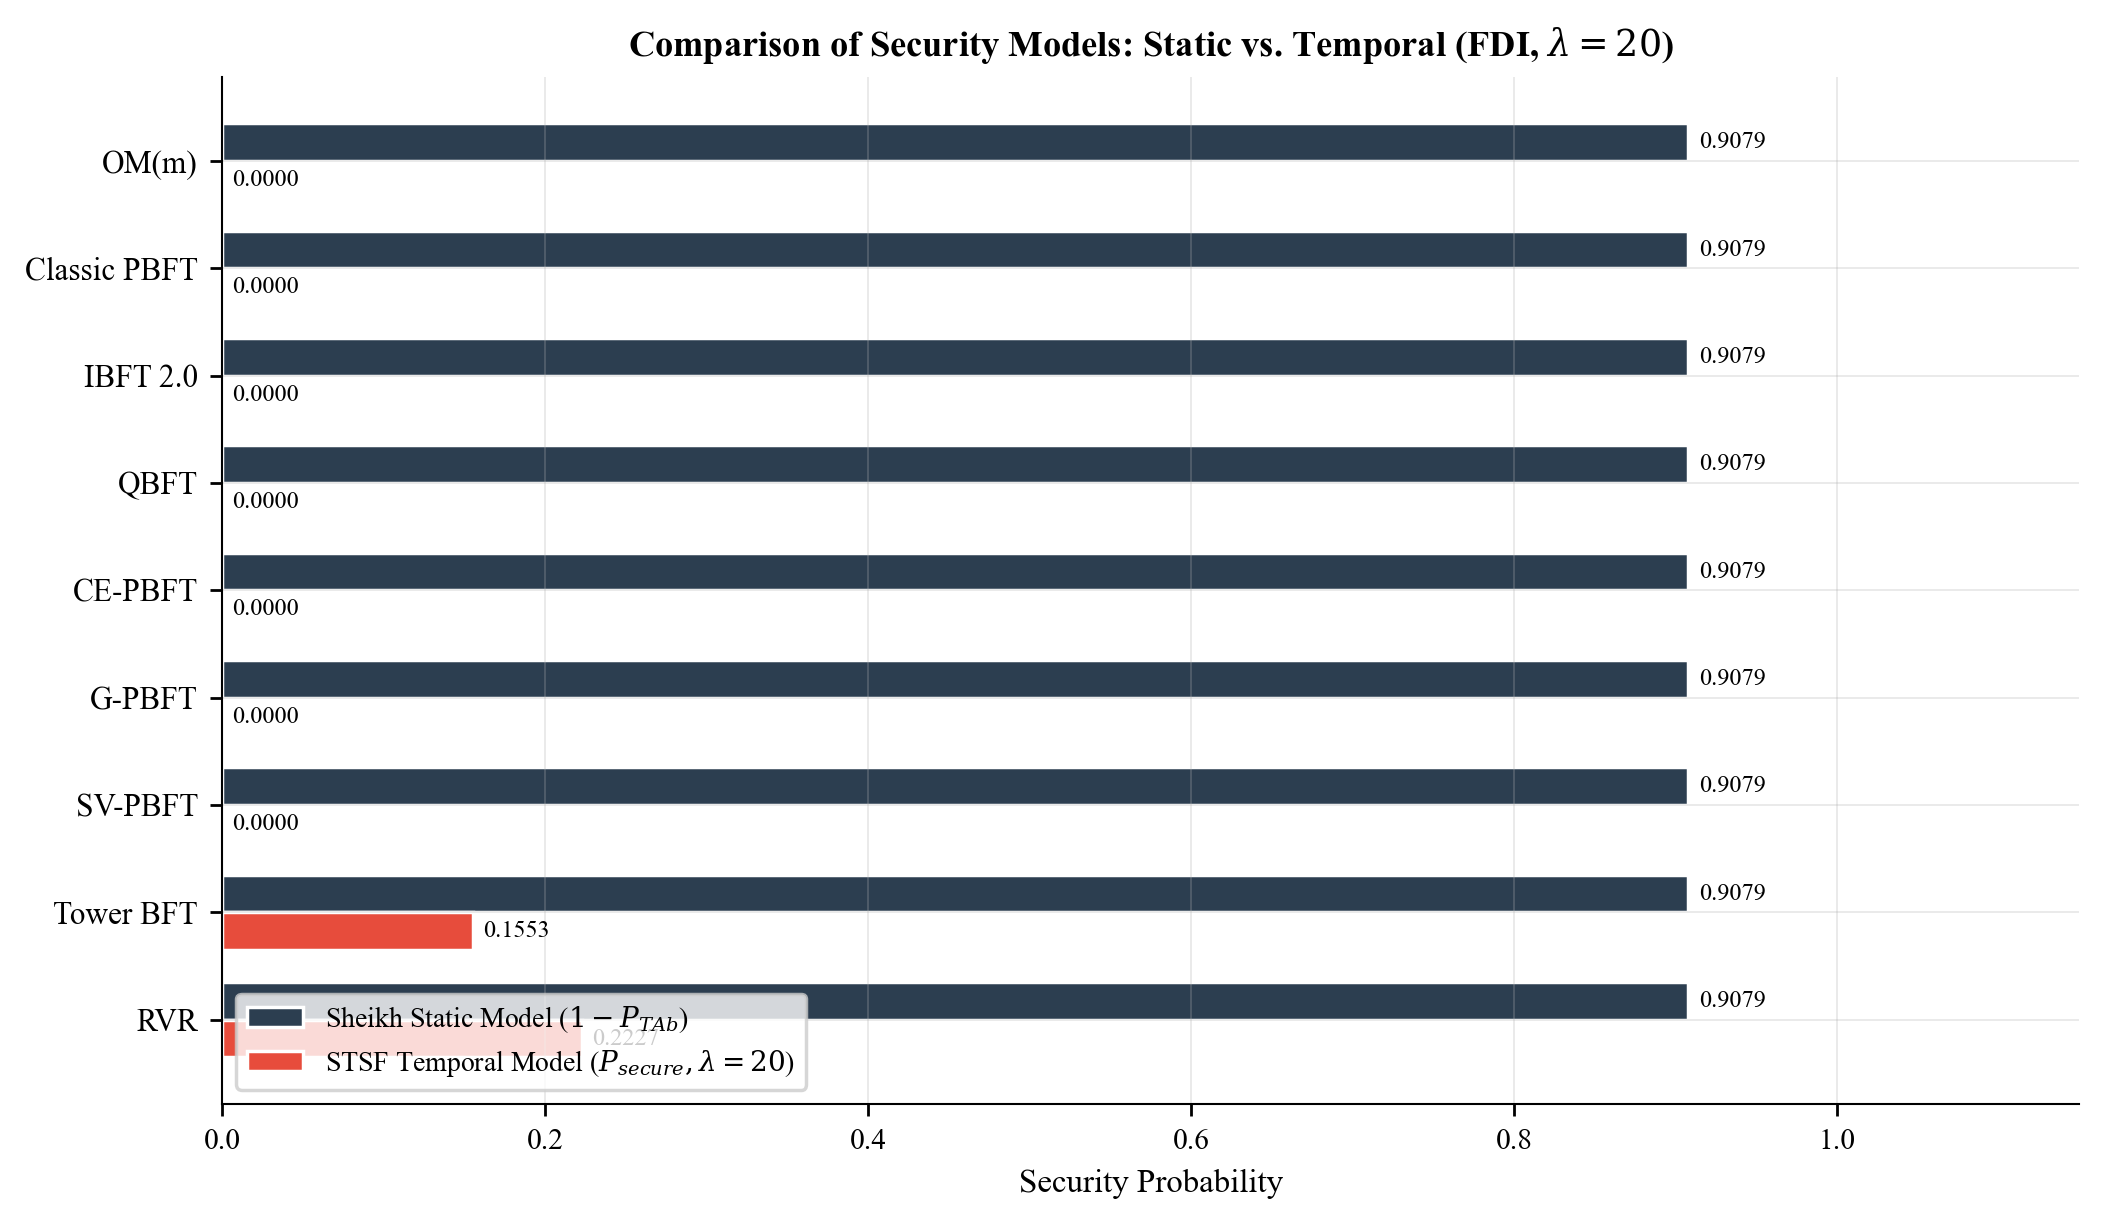
\includegraphics[width=0.75\textwidth]{figures/fig_model_comparison.png}
\end{figure}
\clearpage

\section{Monte Carlo Validation}
\textbf{File:} \texttt{fig\_monte\_carlo\_validation.png} \\
\textbf{Concept/Origin:} This plot visualizes \textbf{Monte Carlo Validation Metric} as a function of \textbf{Time / Baseline Parameter}. \\
\textbf{Equations/Framework:} 
Empirical baseline calculation from simulation data.
\vspace{0.5cm}
\begin{figure}[H]
    \centering
    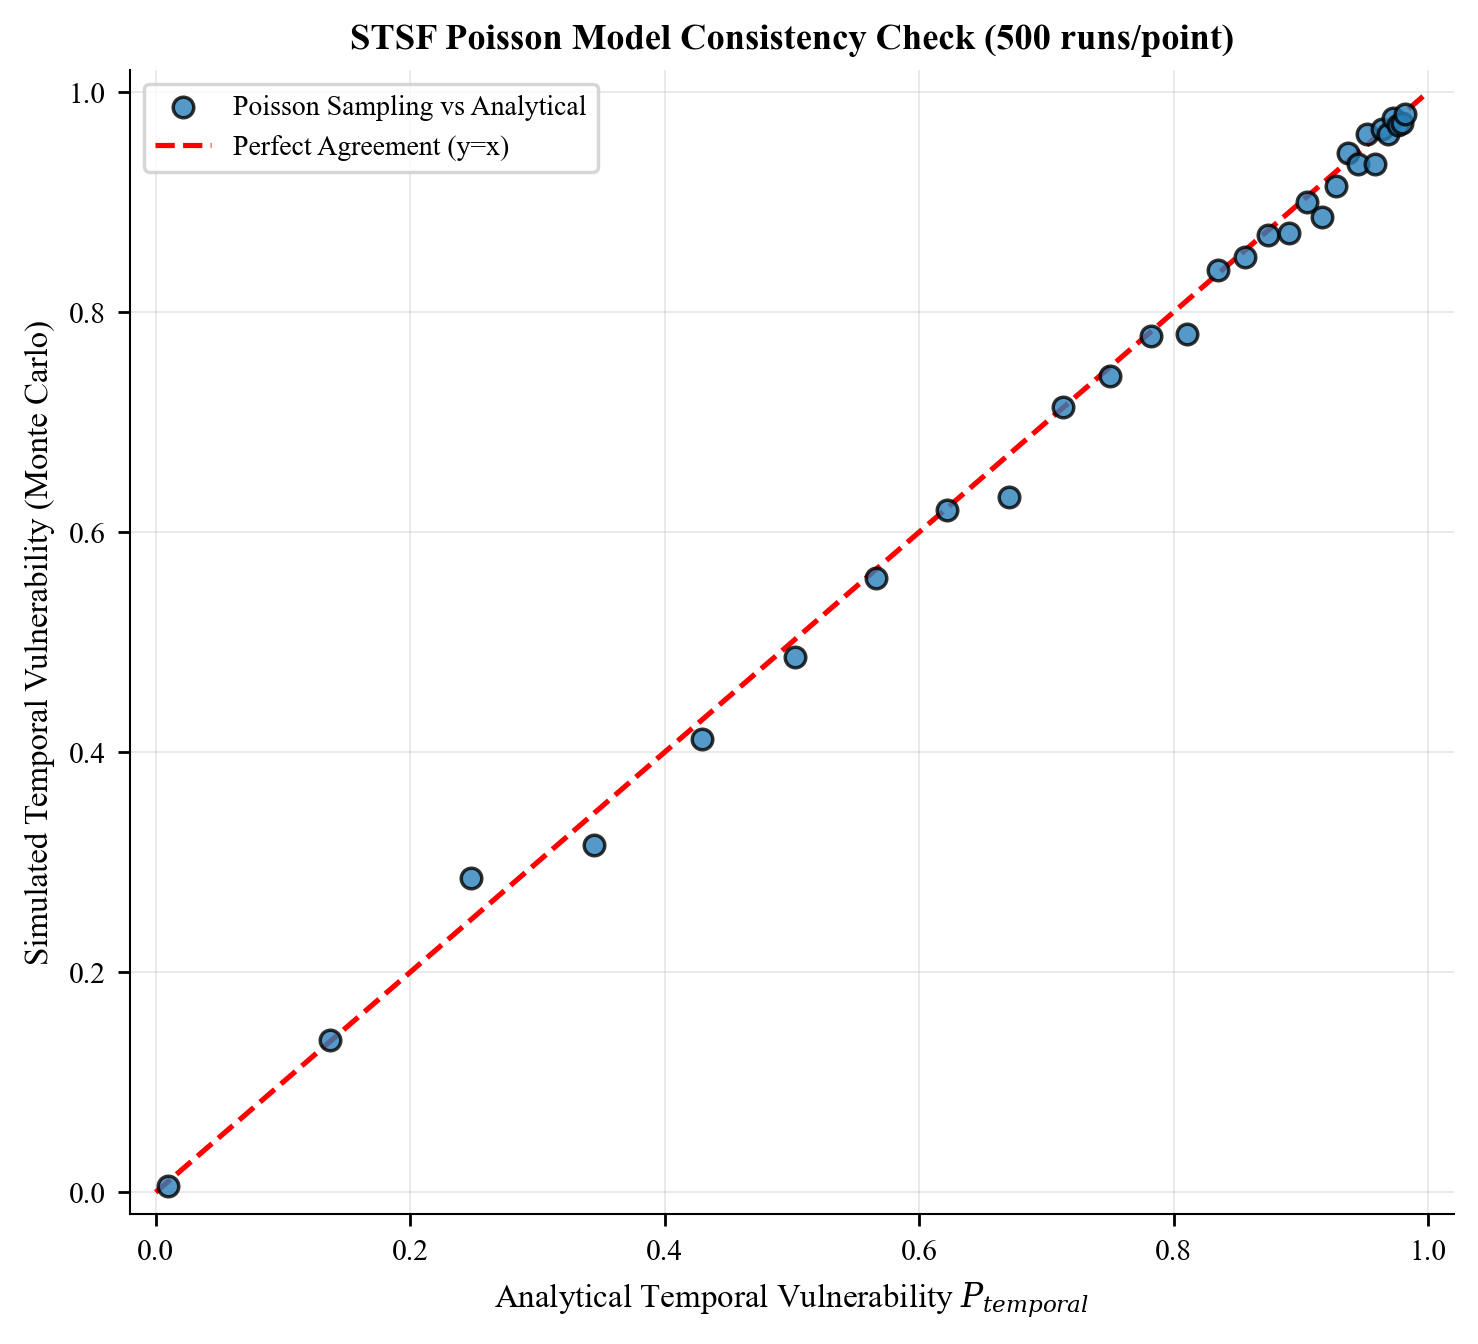
\includegraphics[width=0.75\textwidth]{figures/fig_monte_carlo_validation.png}
\end{figure}
\clearpage

\section{Multi Lambda Comparison}
\textbf{File:} \texttt{fig\_multi\_lambda\_comparison.png} \\
\textbf{Concept/Origin:} This plot visualizes \textbf{Multi Lambda Comparison Metric} as a function of \textbf{Time / Baseline Parameter}. \\
\textbf{Equations/Framework:} 
Empirical baseline calculation from simulation data.
\vspace{0.5cm}
\begin{figure}[H]
    \centering
    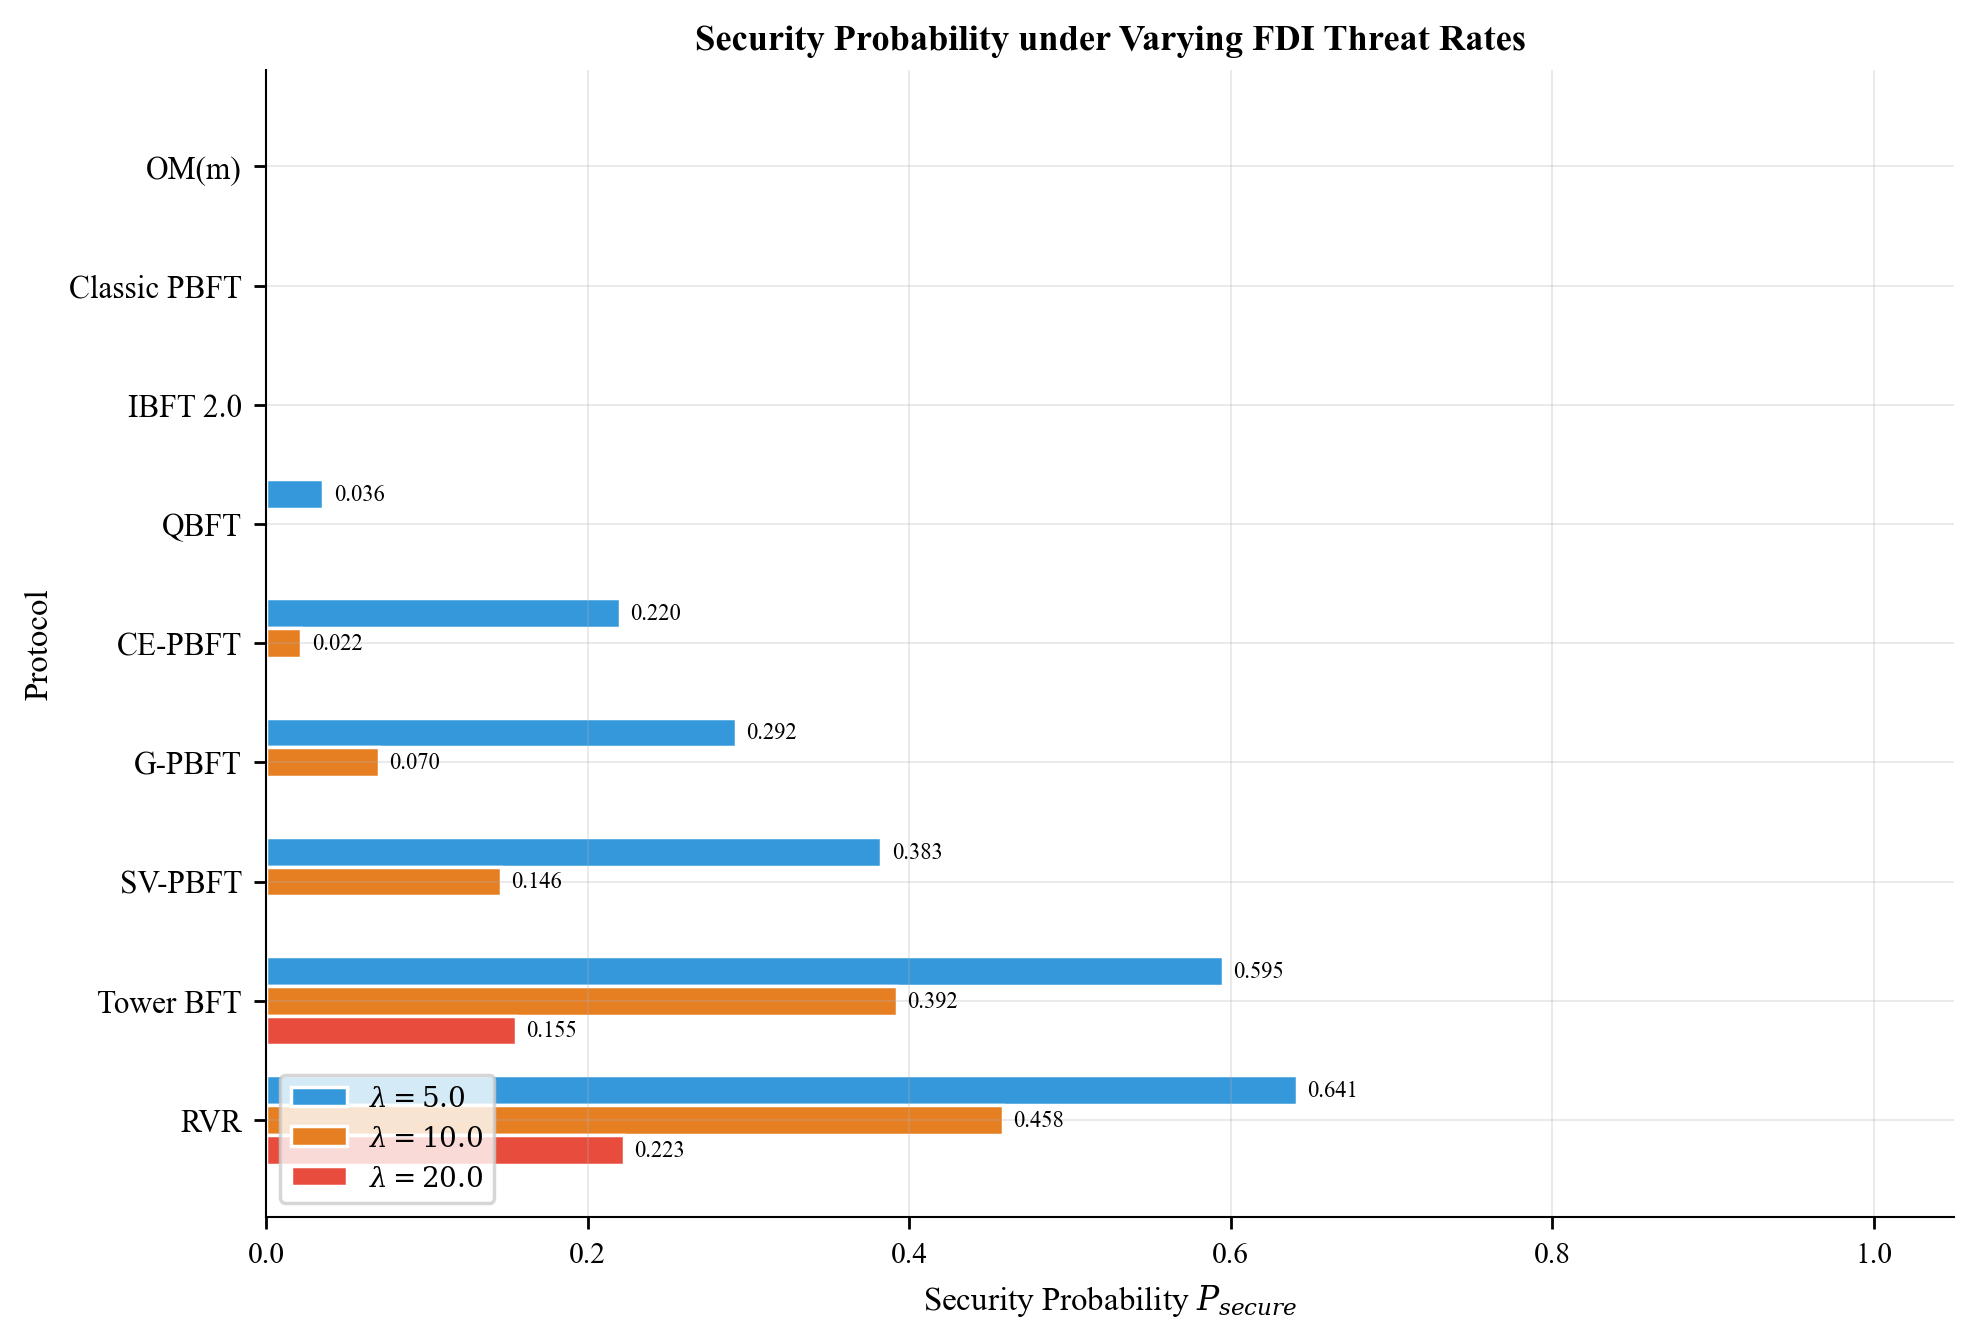
\includegraphics[width=0.75\textwidth]{figures/fig_multi_lambda_comparison.png}
\end{figure}
\clearpage

\section{Pareto Frontier}
\textbf{File:} \texttt{fig\_pareto\_frontier.png} \\
\textbf{Concept/Origin:} This plot visualizes \textbf{Pareto Frontier Metric} as a function of \textbf{Time / Baseline Parameter}. \\
\textbf{Equations/Framework:} 
 P_{secure} = \max( \text{Security} ) \quad \text{s.t.} \quad L_{total} \le L_{max} 
\vspace{0.5cm}
\begin{figure}[H]
    \centering
    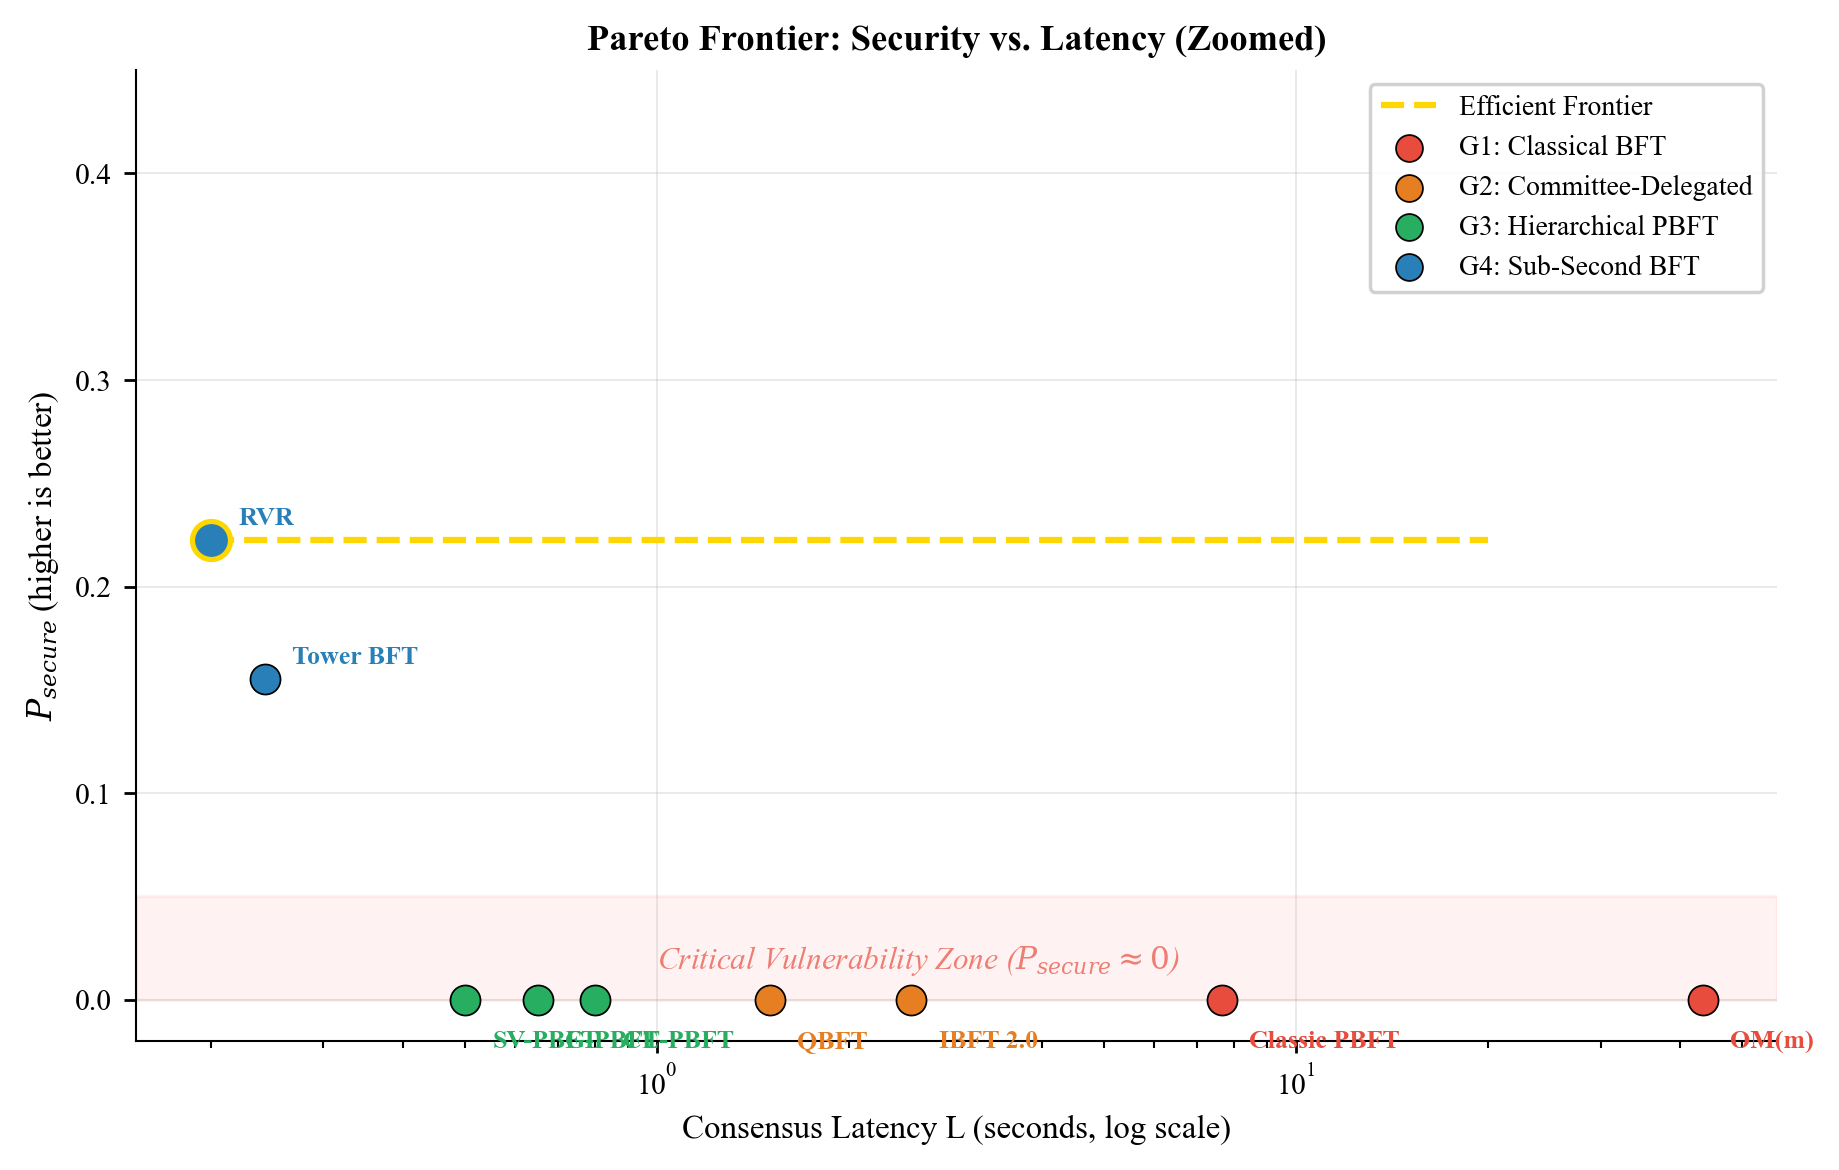
\includegraphics[width=0.75\textwidth]{figures/fig_pareto_frontier.png}
\end{figure}
\clearpage

\section{Ptemporal Vs Latency}
\textbf{File:} \texttt{fig\_ptemporal\_vs\_latency.png} \\
\textbf{Concept/Origin:} This plot visualizes \textbf{Ptemporal} as a function of \textbf{Latency}. \\
\textbf{Equations/Framework:} 
 L_{total} = L_{net} + L_{consensus} 
\vspace{0.5cm}
\begin{figure}[H]
    \centering
    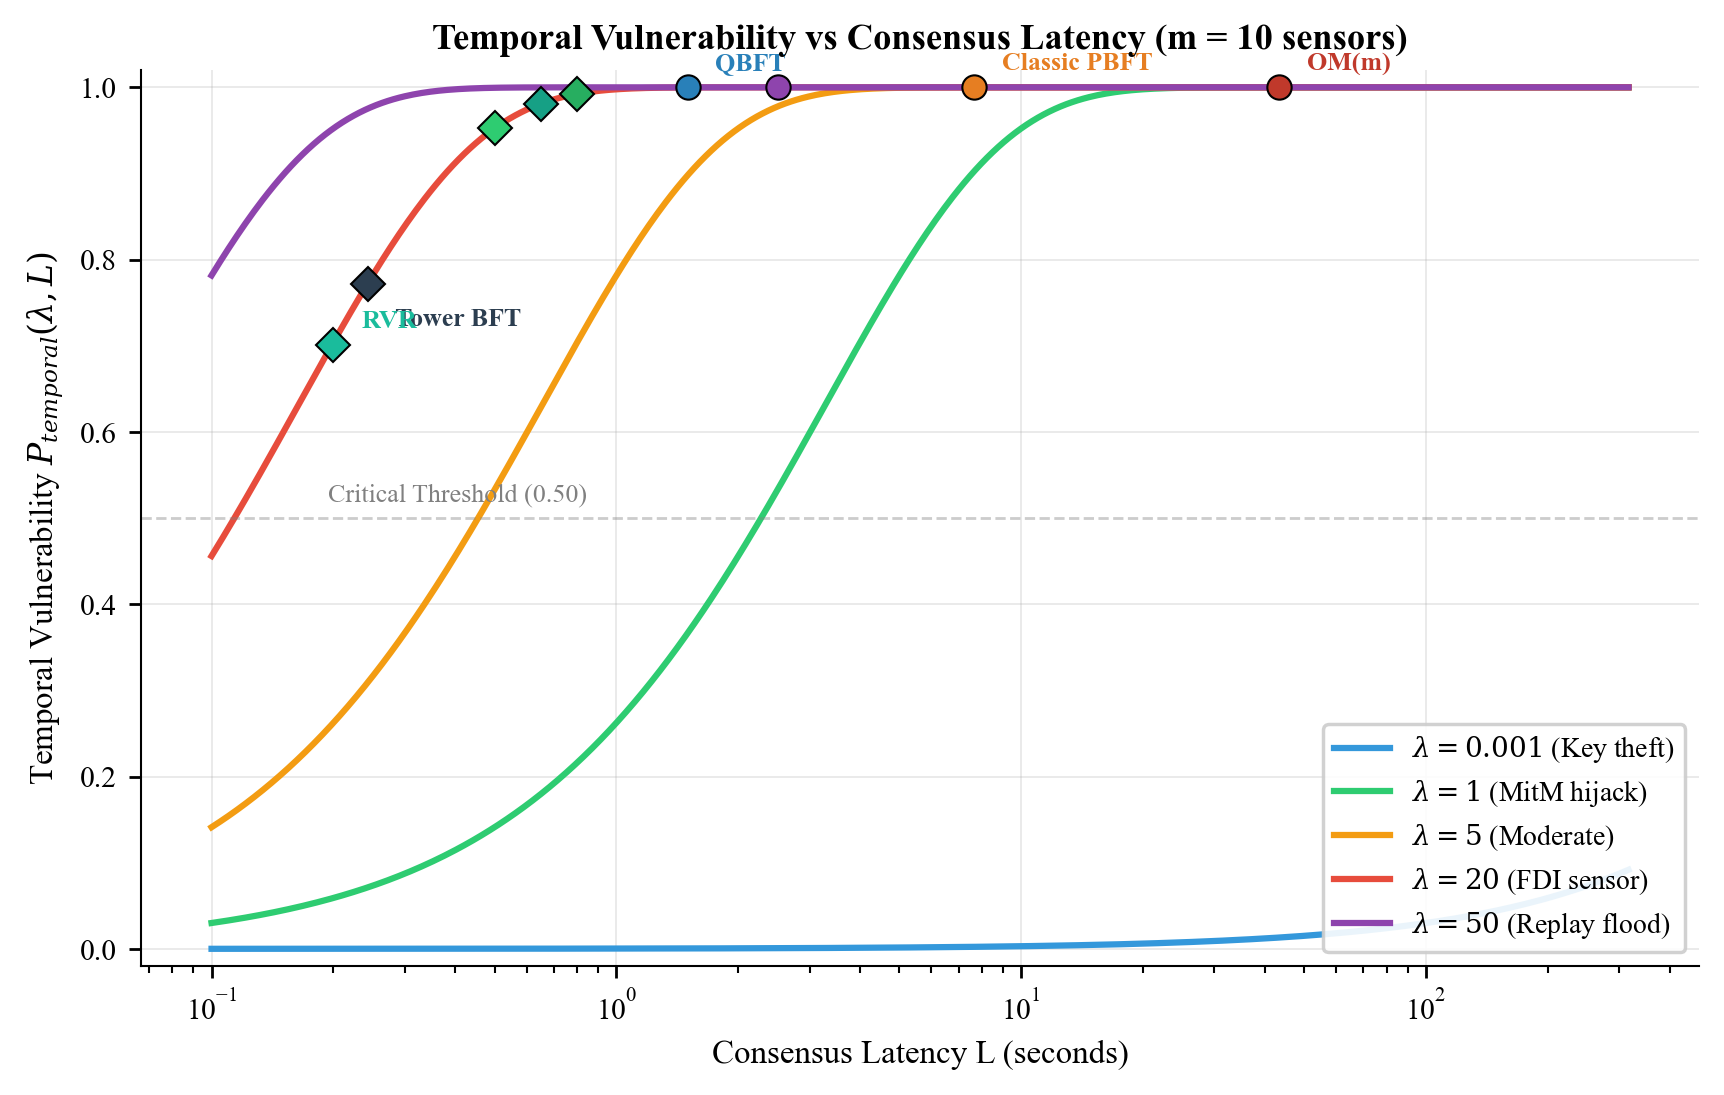
\includegraphics[width=0.75\textwidth]{figures/fig_ptemporal_vs_latency.png}
\end{figure}
\clearpage

\section{Robustness Heatmap}
\textbf{File:} \texttt{fig\_robustness\_heatmap.png} \\
\textbf{Concept/Origin:} This plot visualizes \textbf{Robustness Heatmap Metric} as a function of \textbf{Time / Baseline Parameter}. \\
\textbf{Equations/Framework:} 
 P_{secure} = \max( \text{Security} ) \quad \text{s.t.} \quad L_{total} \le L_{max} 
\vspace{0.5cm}
\begin{figure}[H]
    \centering
    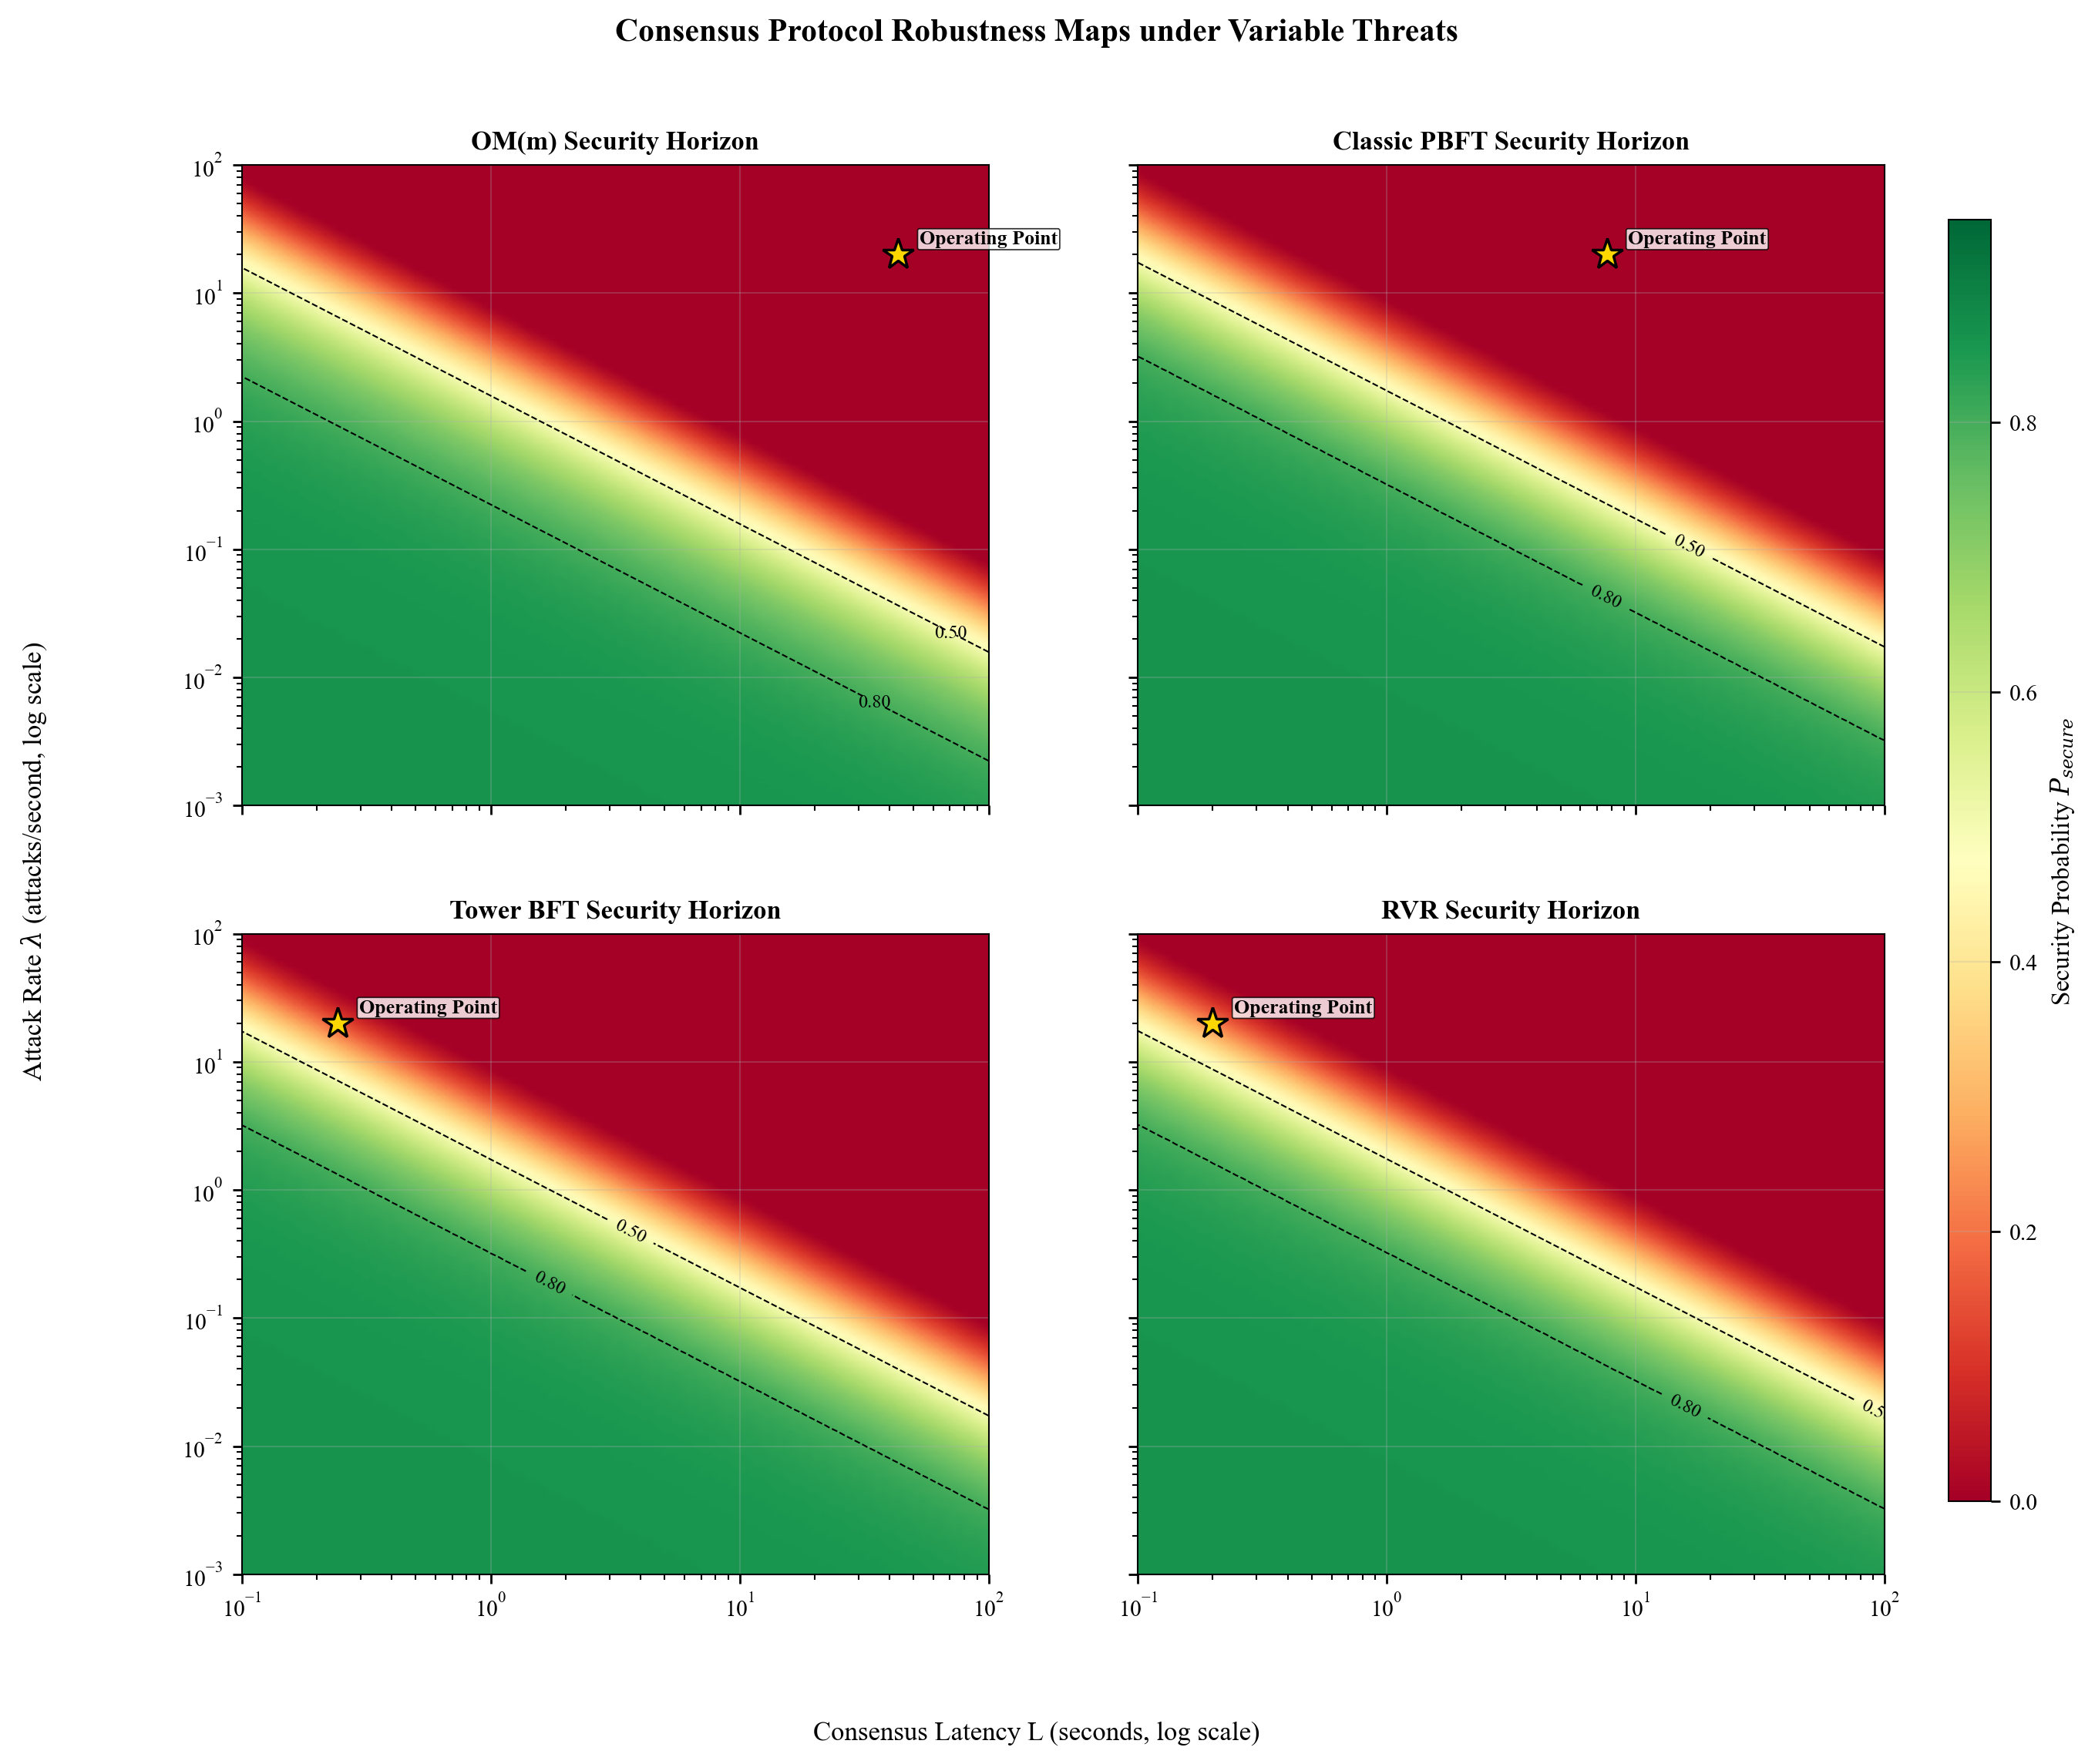
\includegraphics[width=0.75\textwidth]{figures/fig_robustness_heatmap.png}
\end{figure}
\clearpage

\section{Security Gain}
\textbf{File:} \texttt{fig\_security\_gain.png} \\
\textbf{Concept/Origin:} This plot visualizes \textbf{Security Gain Metric} as a function of \textbf{Time / Baseline Parameter}. \\
\textbf{Equations/Framework:} 
Empirical baseline calculation from simulation data.
\vspace{0.5cm}
\begin{figure}[H]
    \centering
    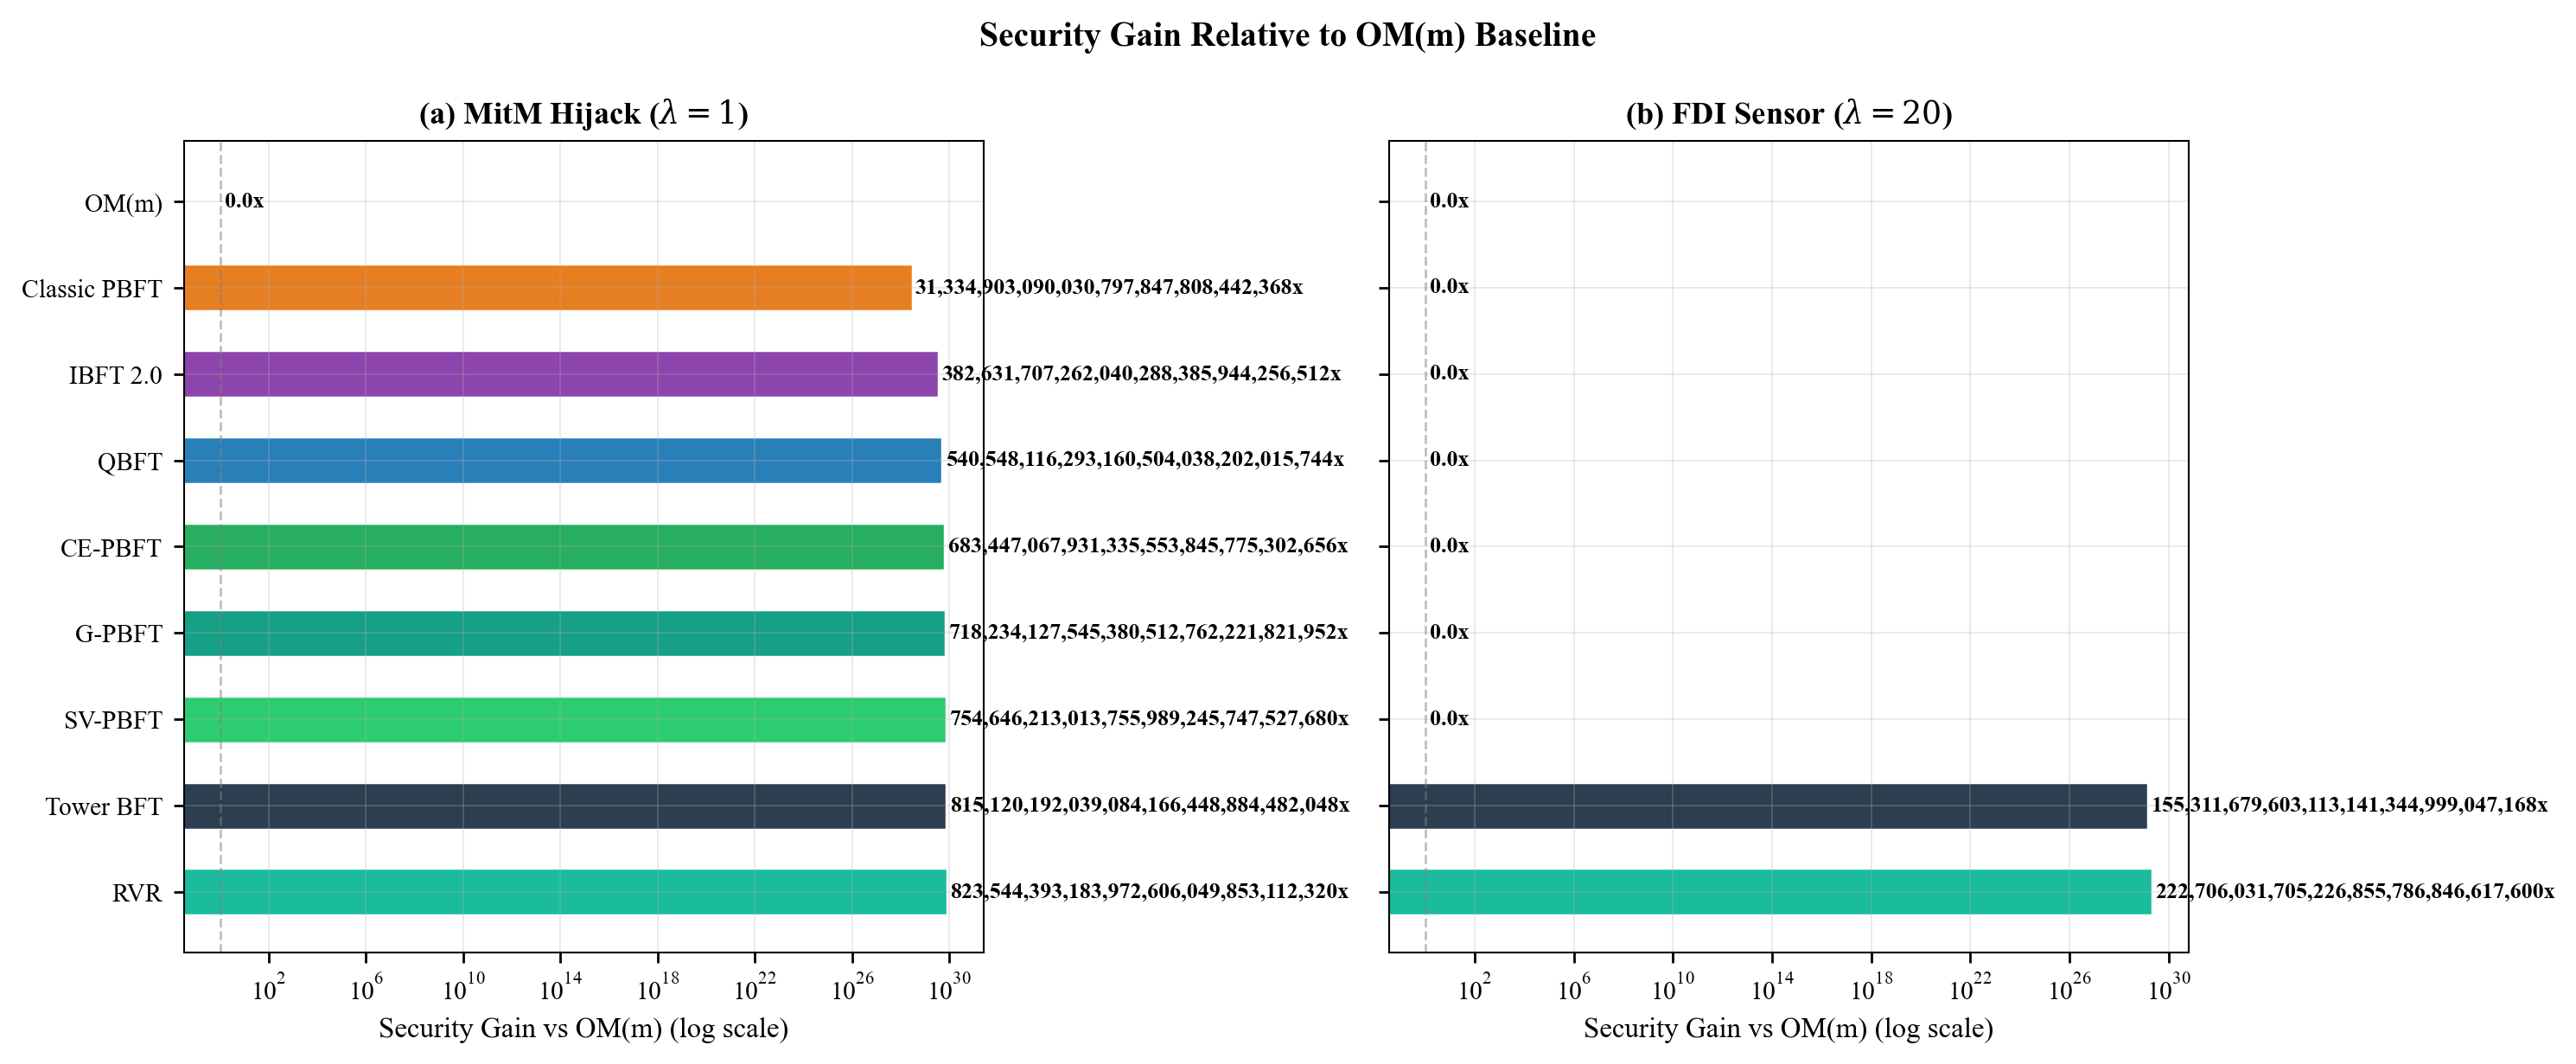
\includegraphics[width=0.75\textwidth]{figures/fig_security_gain.png}
\end{figure}
\clearpage

\section{Sensitivity Lambda}
\textbf{File:} \texttt{fig\_sensitivity\_lambda.png} \\
\textbf{Concept/Origin:} This plot visualizes \textbf{Sensitivity Lambda Metric} as a function of \textbf{Time / Baseline Parameter}. \\
\textbf{Equations/Framework:} 
Empirical baseline calculation from simulation data.
\vspace{0.5cm}
\begin{figure}[H]
    \centering
    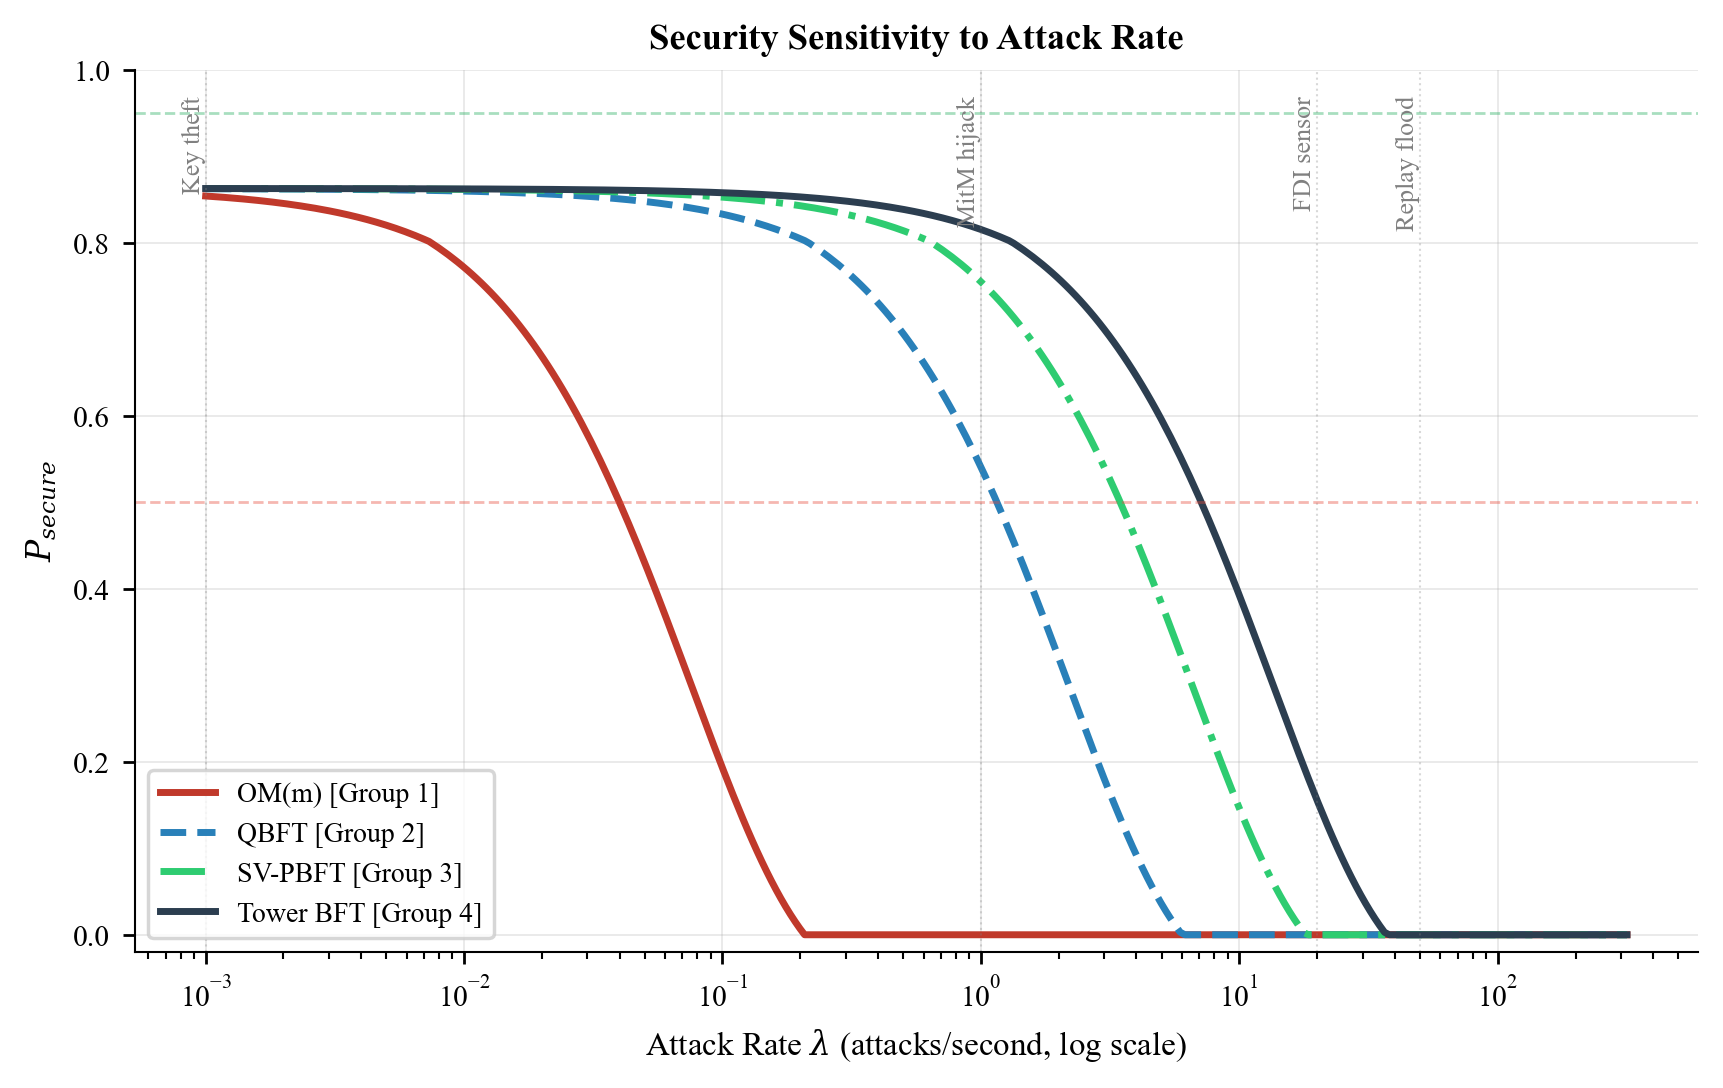
\includegraphics[width=0.75\textwidth]{figures/fig_sensitivity_lambda.png}
\end{figure}
\clearpage

\section{Sensitivity Ranking}
\textbf{File:} \texttt{fig\_sensitivity\_ranking.png} \\
\textbf{Concept/Origin:} This plot visualizes \textbf{Sensitivity Ranking Metric} as a function of \textbf{Time / Baseline Parameter}. \\
\textbf{Equations/Framework:} 
Empirical baseline calculation from simulation data.
\vspace{0.5cm}
\begin{figure}[H]
    \centering
    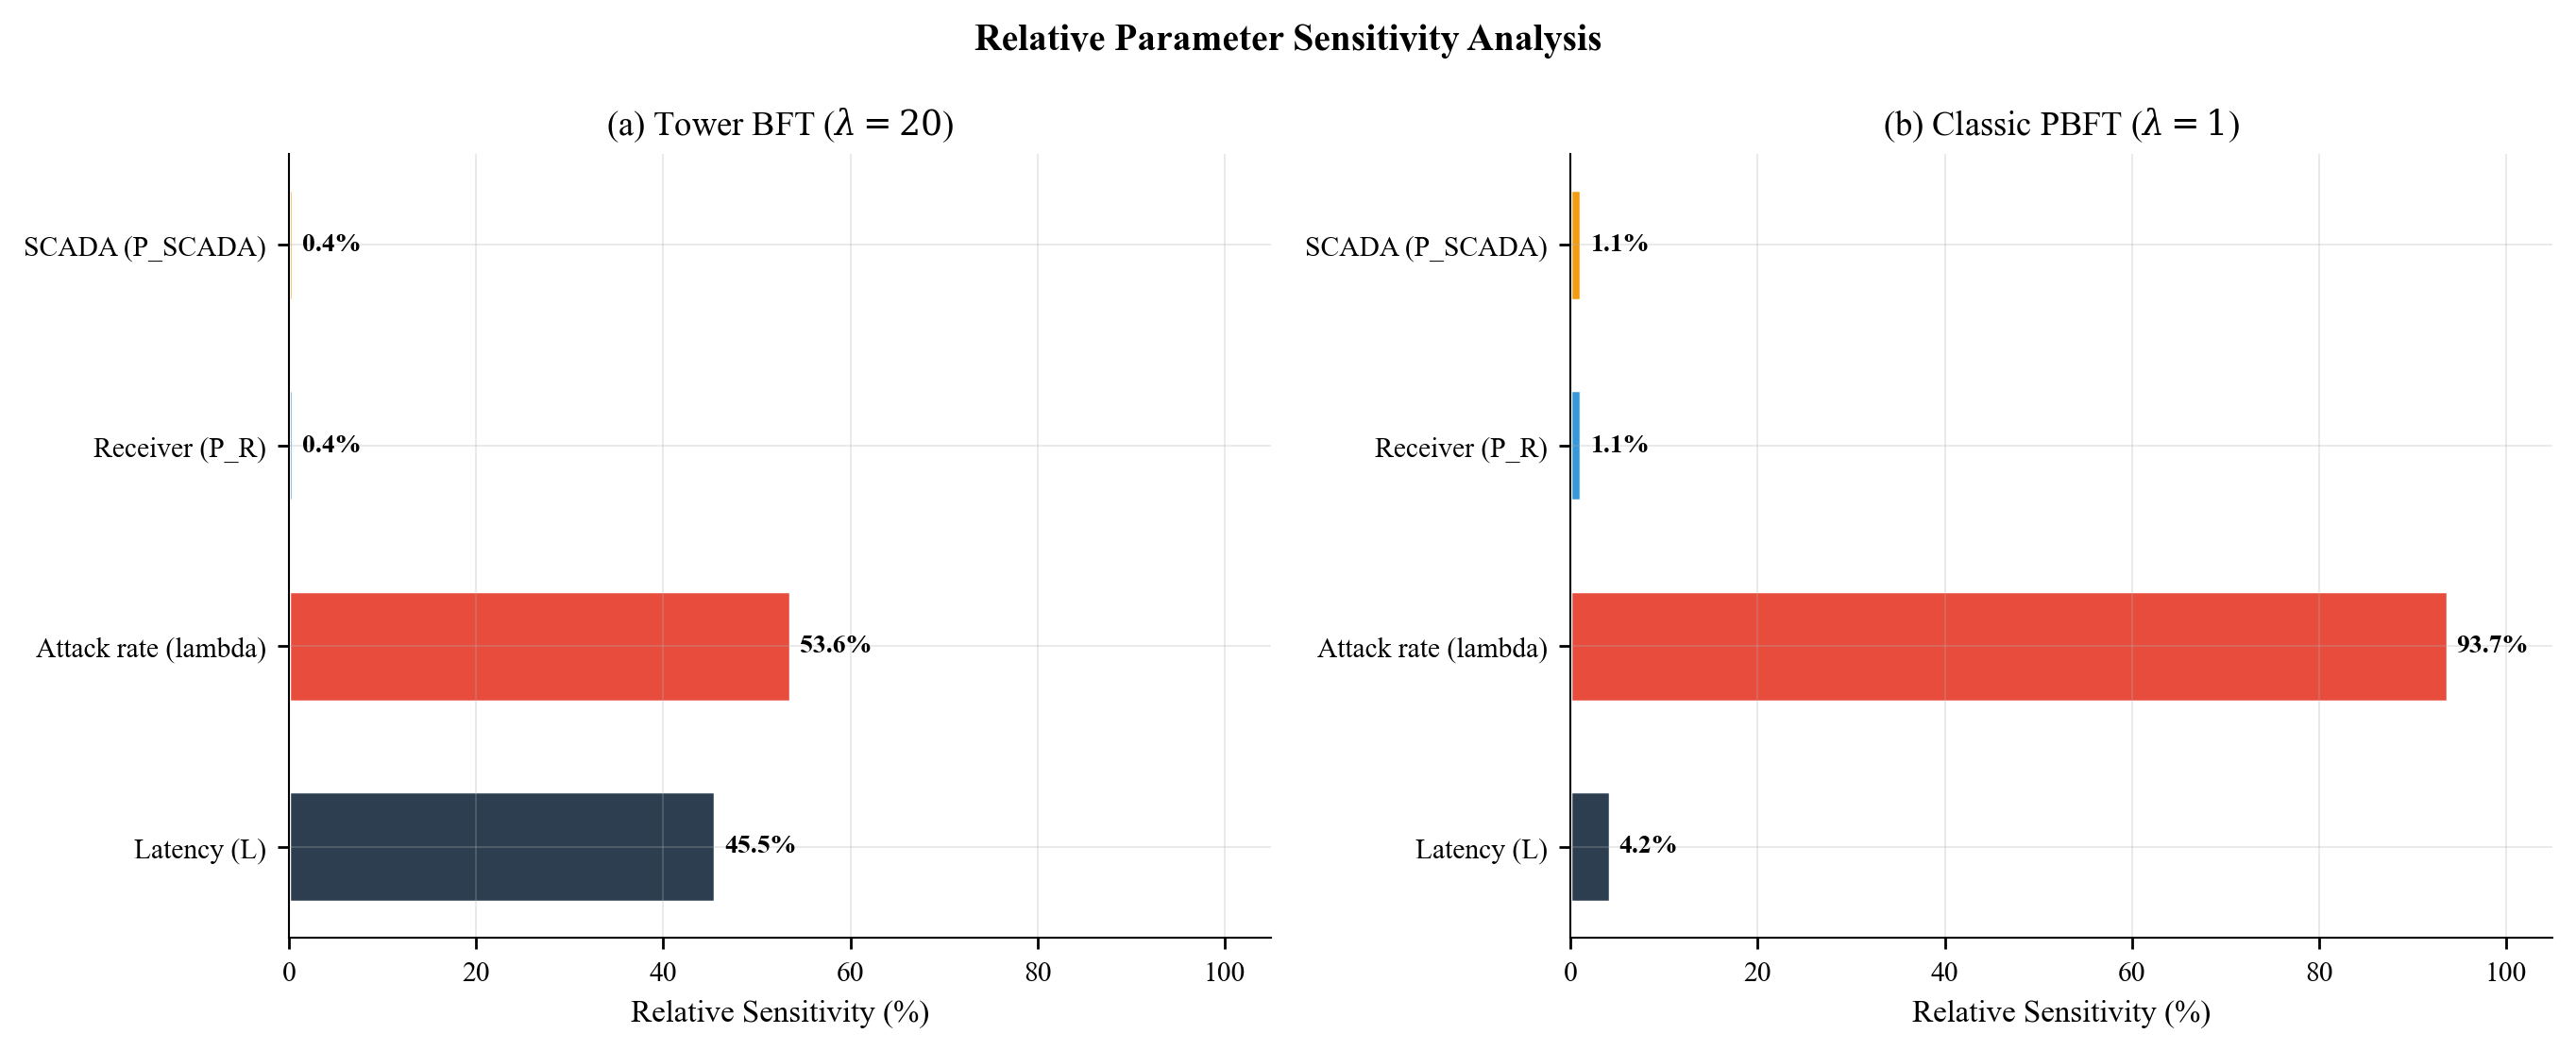
\includegraphics[width=0.75\textwidth]{figures/fig_sensitivity_ranking.png}
\end{figure}
\clearpage

\section{Sensor Sensitivity}
\textbf{File:} \texttt{fig\_sensor\_sensitivity.png} \\
\textbf{Concept/Origin:} This plot visualizes \textbf{Sensor Sensitivity Metric} as a function of \textbf{Time / Baseline Parameter}. \\
\textbf{Equations/Framework:} 
Empirical baseline calculation from simulation data.
\vspace{0.5cm}
\begin{figure}[H]
    \centering
    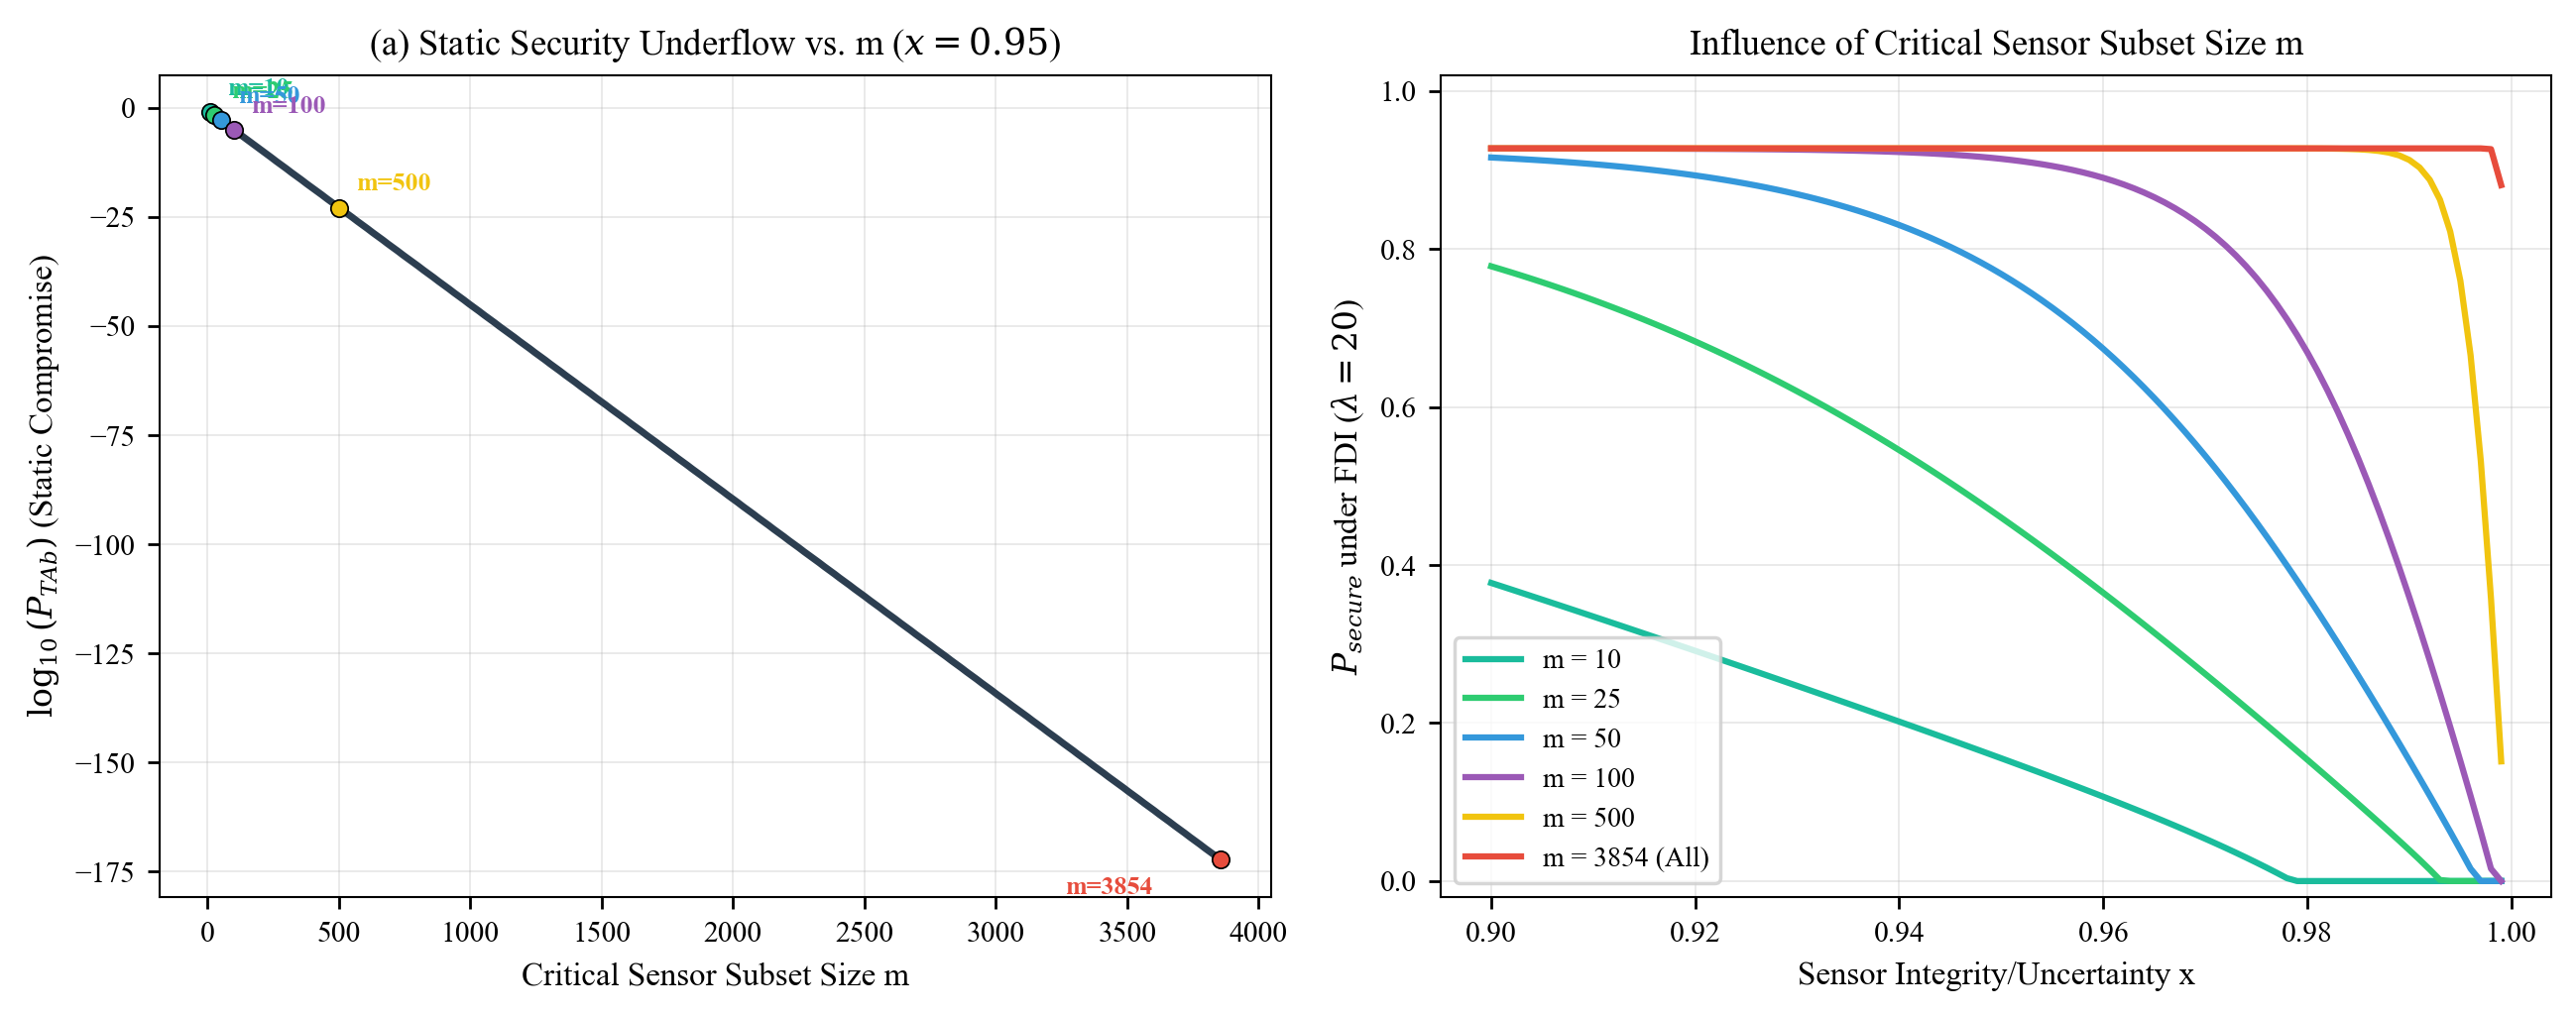
\includegraphics[width=0.75\textwidth]{figures/fig_sensor_sensitivity.png}
\end{figure}
\clearpage

\section{Spof Risk}
\textbf{File:} \texttt{fig\_spof\_risk.png} \\
\textbf{Concept/Origin:} This plot visualizes \textbf{Spof Risk Metric} as a function of \textbf{Time / Baseline Parameter}. \\
\textbf{Equations/Framework:} 
 P_{Byz} = \sum_{i=f+1}^{n} \binom{n}{i} p_c^i (1-p_c)^{n-i} 
 P_{temporal} = 1 - e^{-\lambda L P_{TA}} 
\vspace{0.5cm}
\begin{figure}[H]
    \centering
    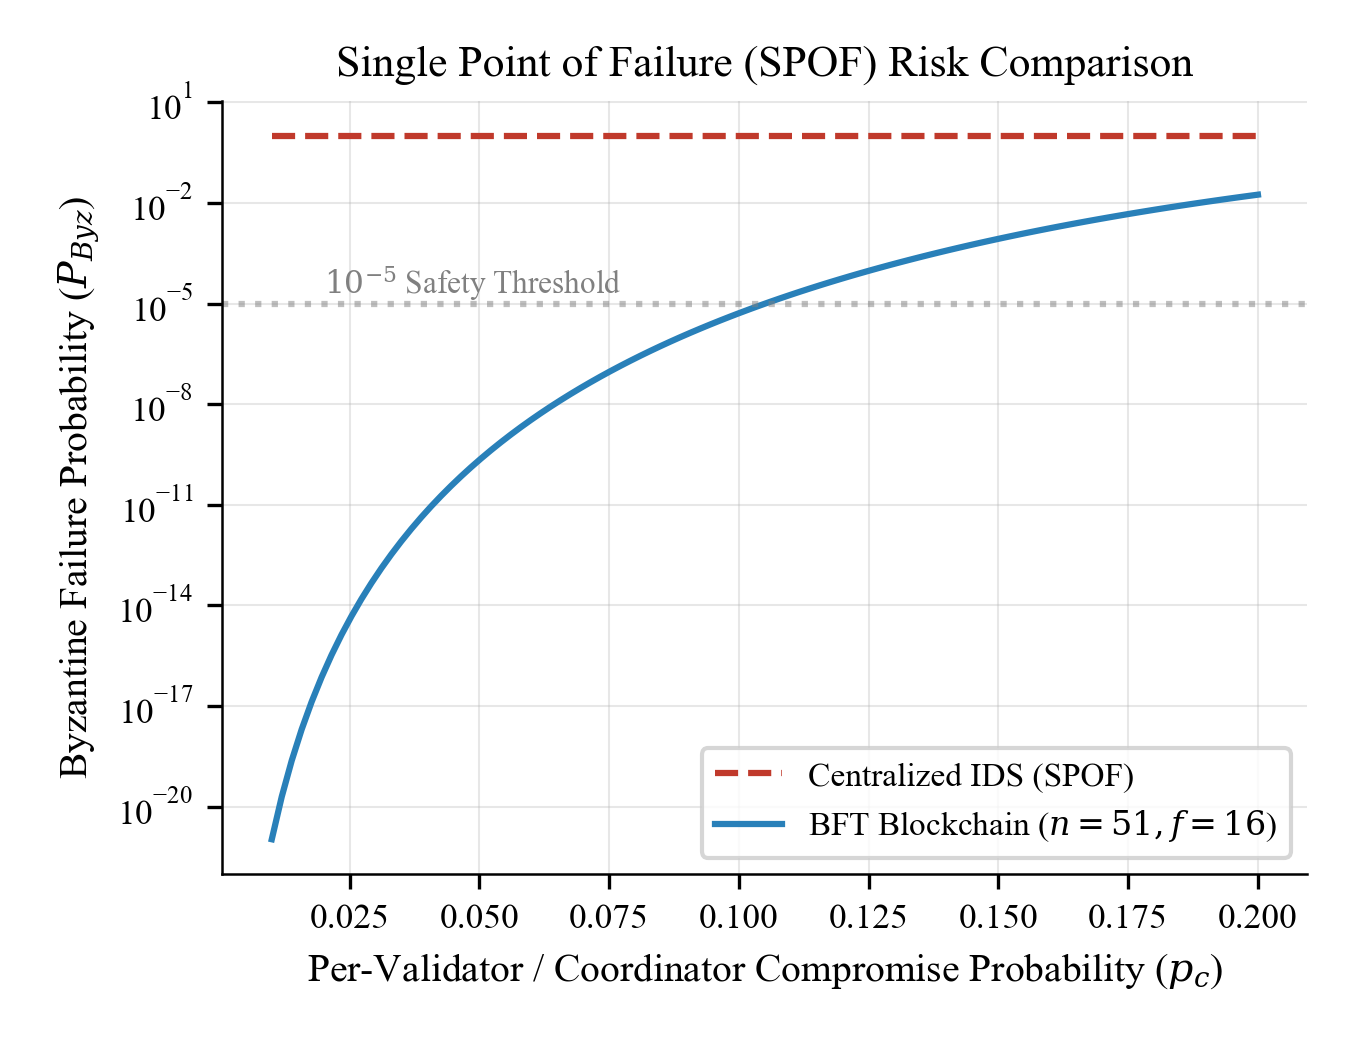
\includegraphics[width=0.75\textwidth]{figures/fig_spof_risk.png}
\end{figure}
\clearpage

\section{W Bft Vs Tbft Attack}
\textbf{File:} \texttt{fig\_w2\_bft\_vs\_tbft\_attack.png} \\
\textbf{Concept/Origin:} This plot visualizes \textbf{W Bft} as a function of \textbf{Tbft Attack}. \\
\textbf{Equations/Framework:} 
Empirical baseline calculation from simulation data.
\vspace{0.5cm}
\begin{figure}[H]
    \centering
    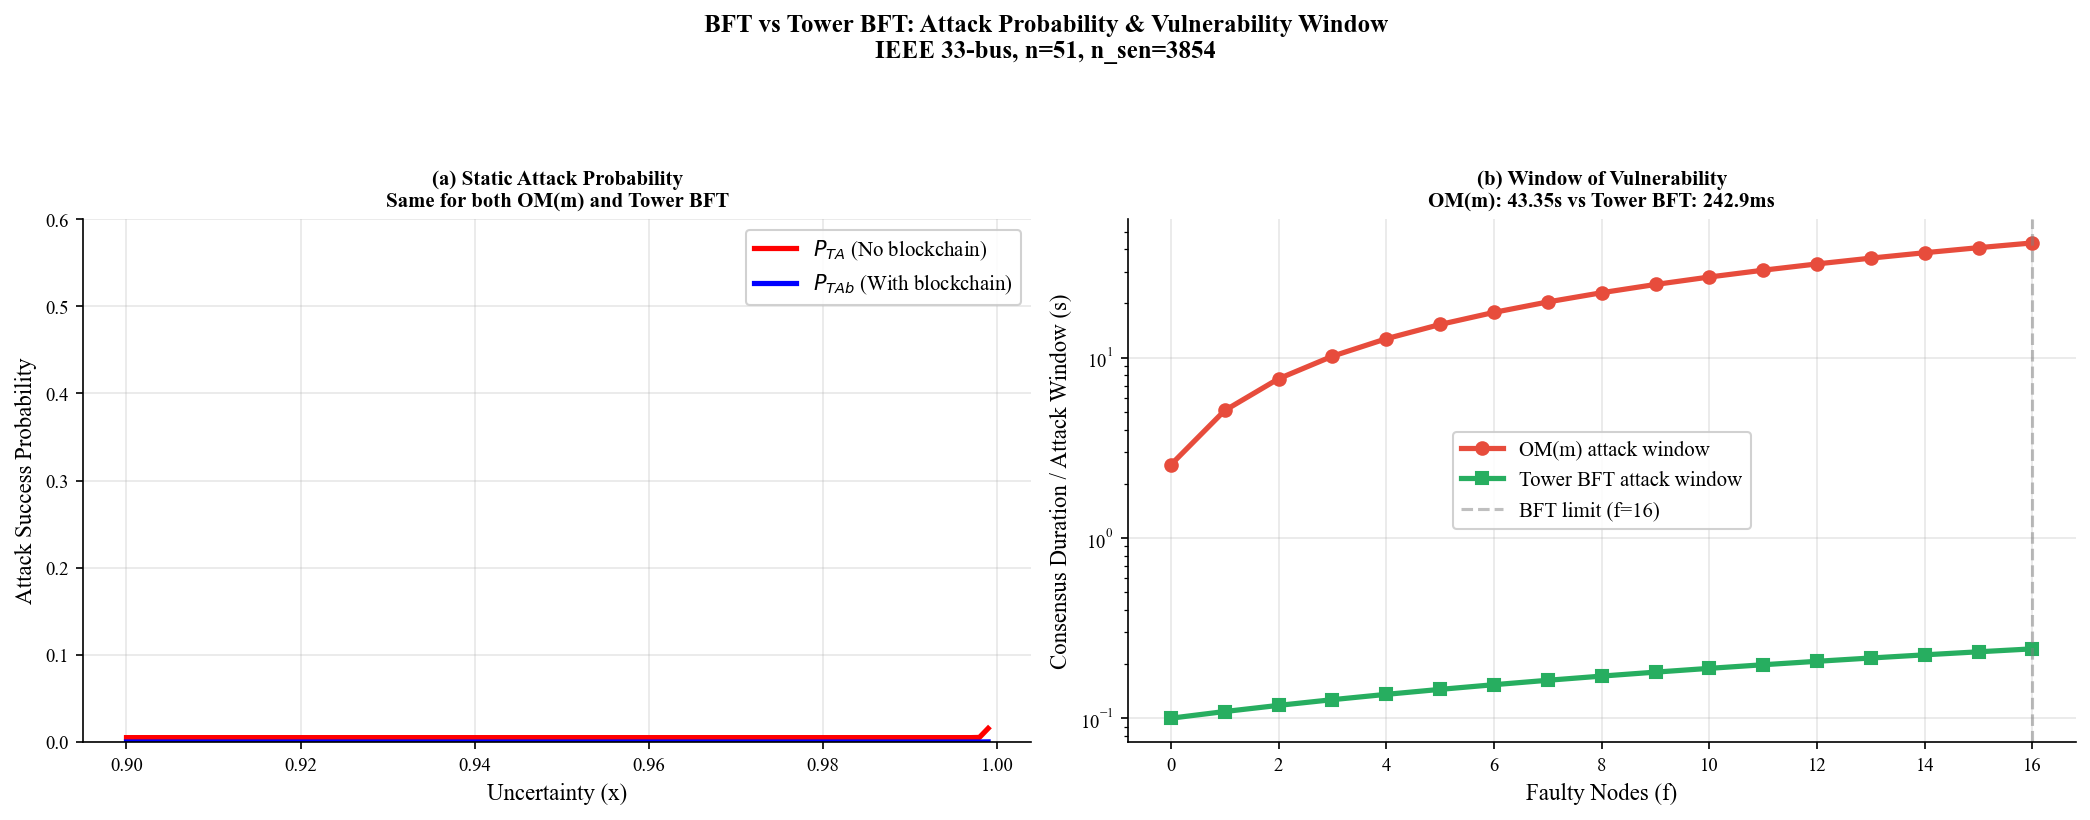
\includegraphics[width=0.75\textwidth]{figures/fig_w2_bft_vs_tbft_attack.png}
\end{figure}
\clearpage

\section{W Pta No Blockchain}
\textbf{File:} \texttt{fig\_w2\_pta\_no\_blockchain.png} \\
\textbf{Concept/Origin:} This plot visualizes \textbf{W Pta No Blockchain Metric} as a function of \textbf{Time / Baseline Parameter}. \\
\textbf{Equations/Framework:} 
Empirical baseline calculation from simulation data.
\vspace{0.5cm}
\begin{figure}[H]
    \centering
    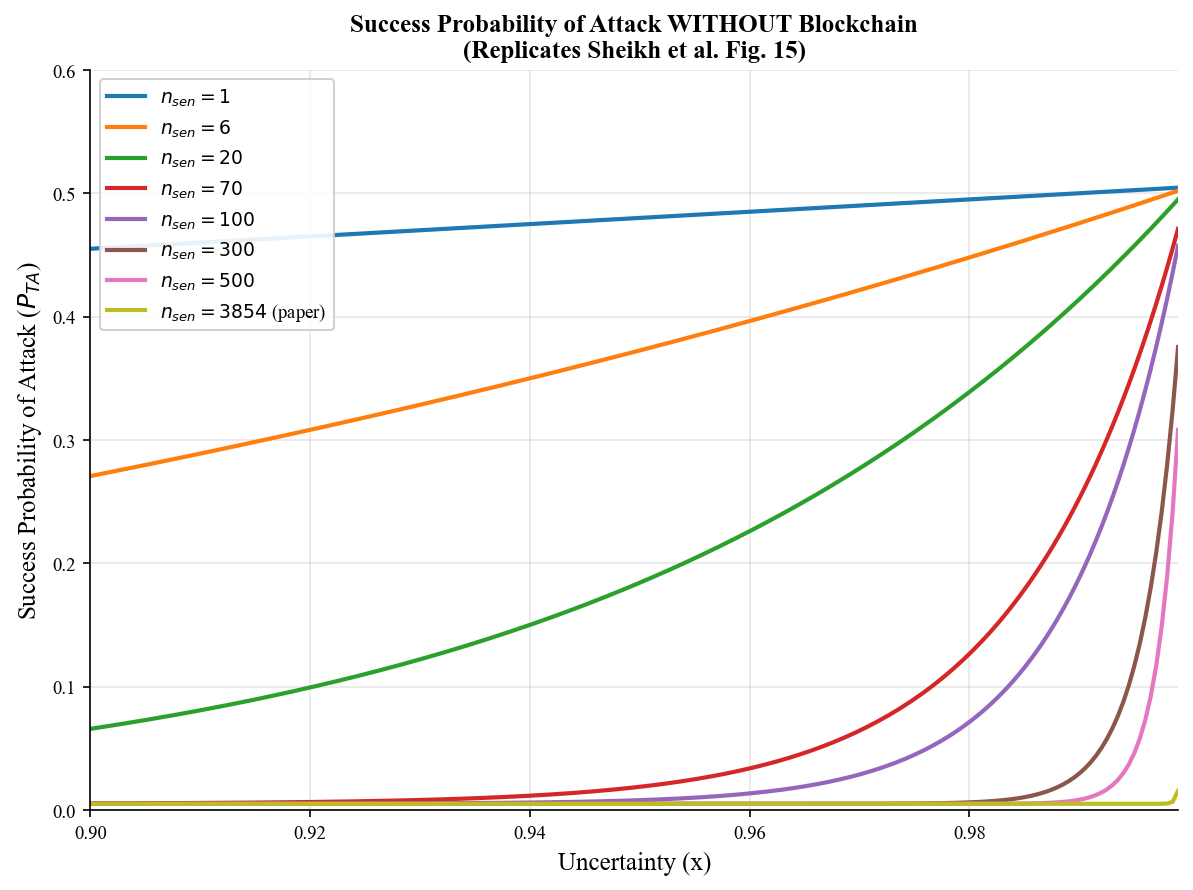
\includegraphics[width=0.75\textwidth]{figures/fig_w2_pta_no_blockchain.png}
\end{figure}
\clearpage

\section{W Ptab With Blockchain}
\textbf{File:} \texttt{fig\_w2\_ptab\_with\_blockchain.png} \\
\textbf{Concept/Origin:} This plot visualizes \textbf{W Ptab With Blockchain Metric} as a function of \textbf{Time / Baseline Parameter}. \\
\textbf{Equations/Framework:} 
Empirical baseline calculation from simulation data.
\vspace{0.5cm}
\begin{figure}[H]
    \centering
    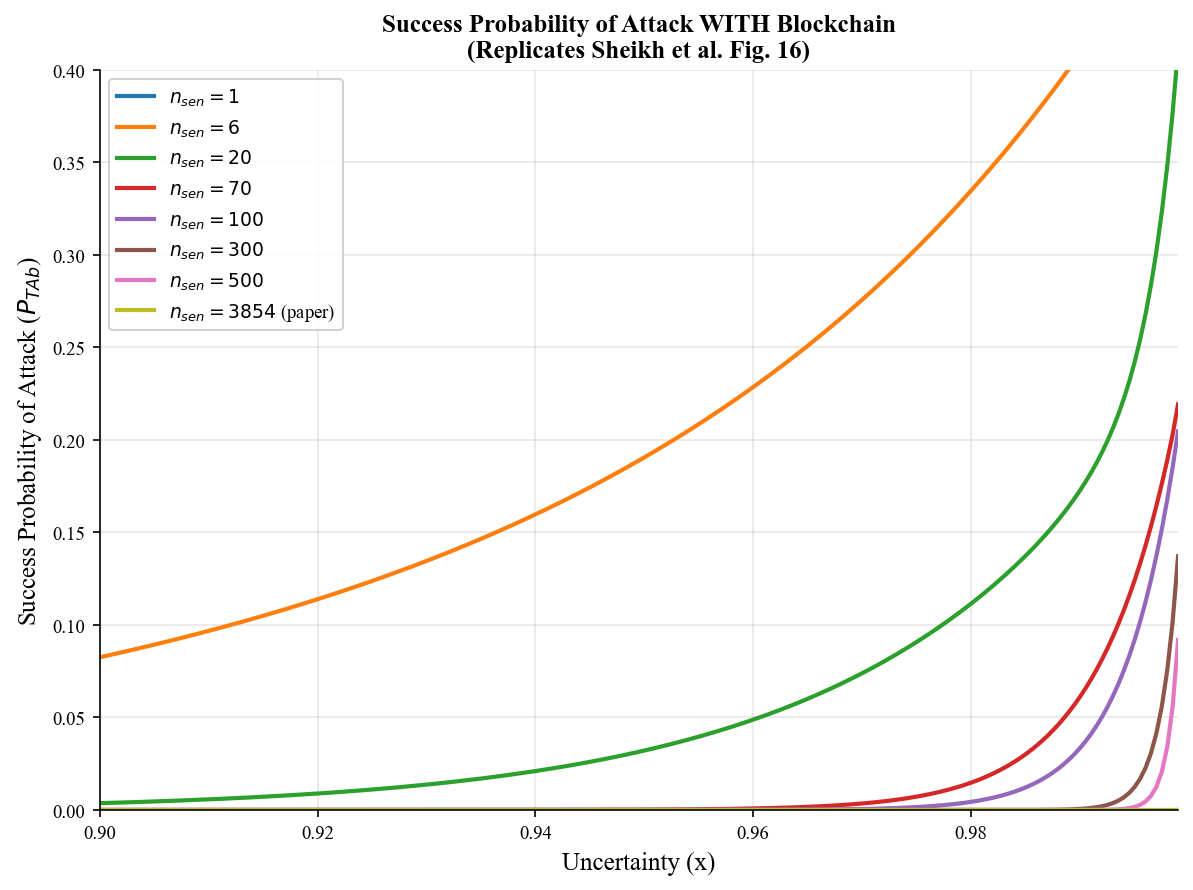
\includegraphics[width=0.75\textwidth]{figures/fig_w2_ptab_with_blockchain.png}
\end{figure}
\clearpage

\section{W Scenario Energy}
\textbf{File:} \texttt{fig\_w2\_scenario1\_energy.png} \\
\textbf{Concept/Origin:} This plot visualizes \textbf{W Scenario Energy Metric} as a function of \textbf{Time / Baseline Parameter}. \\
\textbf{Equations/Framework:} 
 E_{total} = E_{tx} + E_{rx} + E_{crypto} 
\vspace{0.5cm}
\begin{figure}[H]
    \centering
    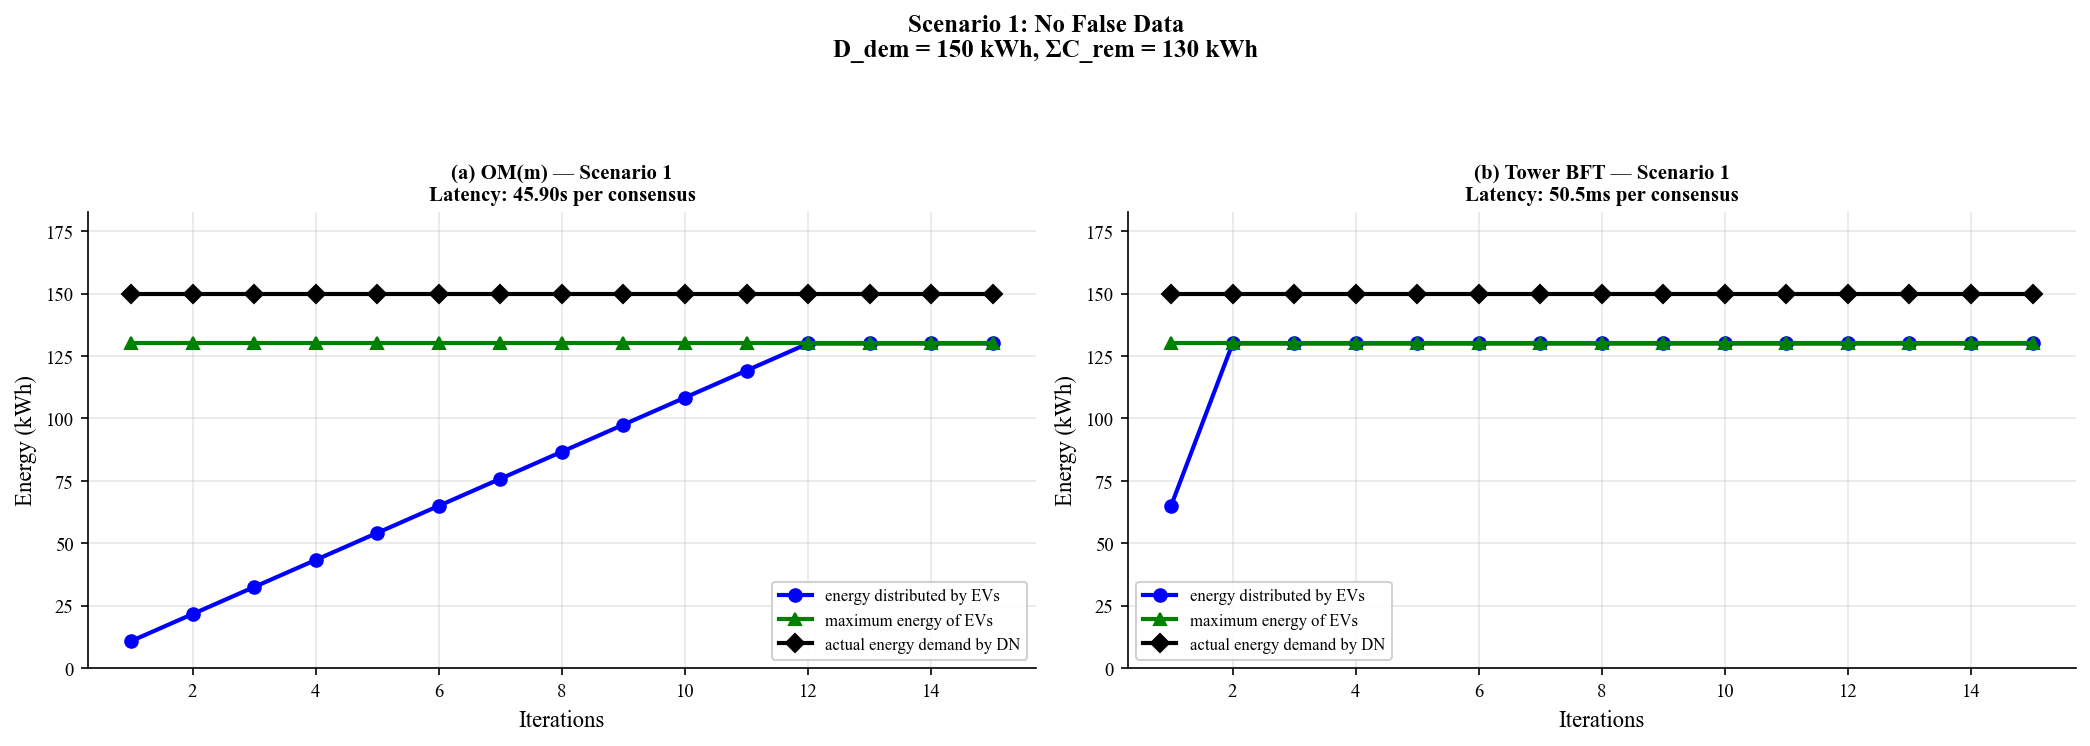
\includegraphics[width=0.75\textwidth]{figures/fig_w2_scenario1_energy.png}
\end{figure}
\clearpage

\section{W Scenario Energy}
\textbf{File:} \texttt{fig\_w2\_scenario2\_energy.png} \\
\textbf{Concept/Origin:} This plot visualizes \textbf{W Scenario Energy Metric} as a function of \textbf{Time / Baseline Parameter}. \\
\textbf{Equations/Framework:} 
 E_{total} = E_{tx} + E_{rx} + E_{crypto} 
\vspace{0.5cm}
\begin{figure}[H]
    \centering
    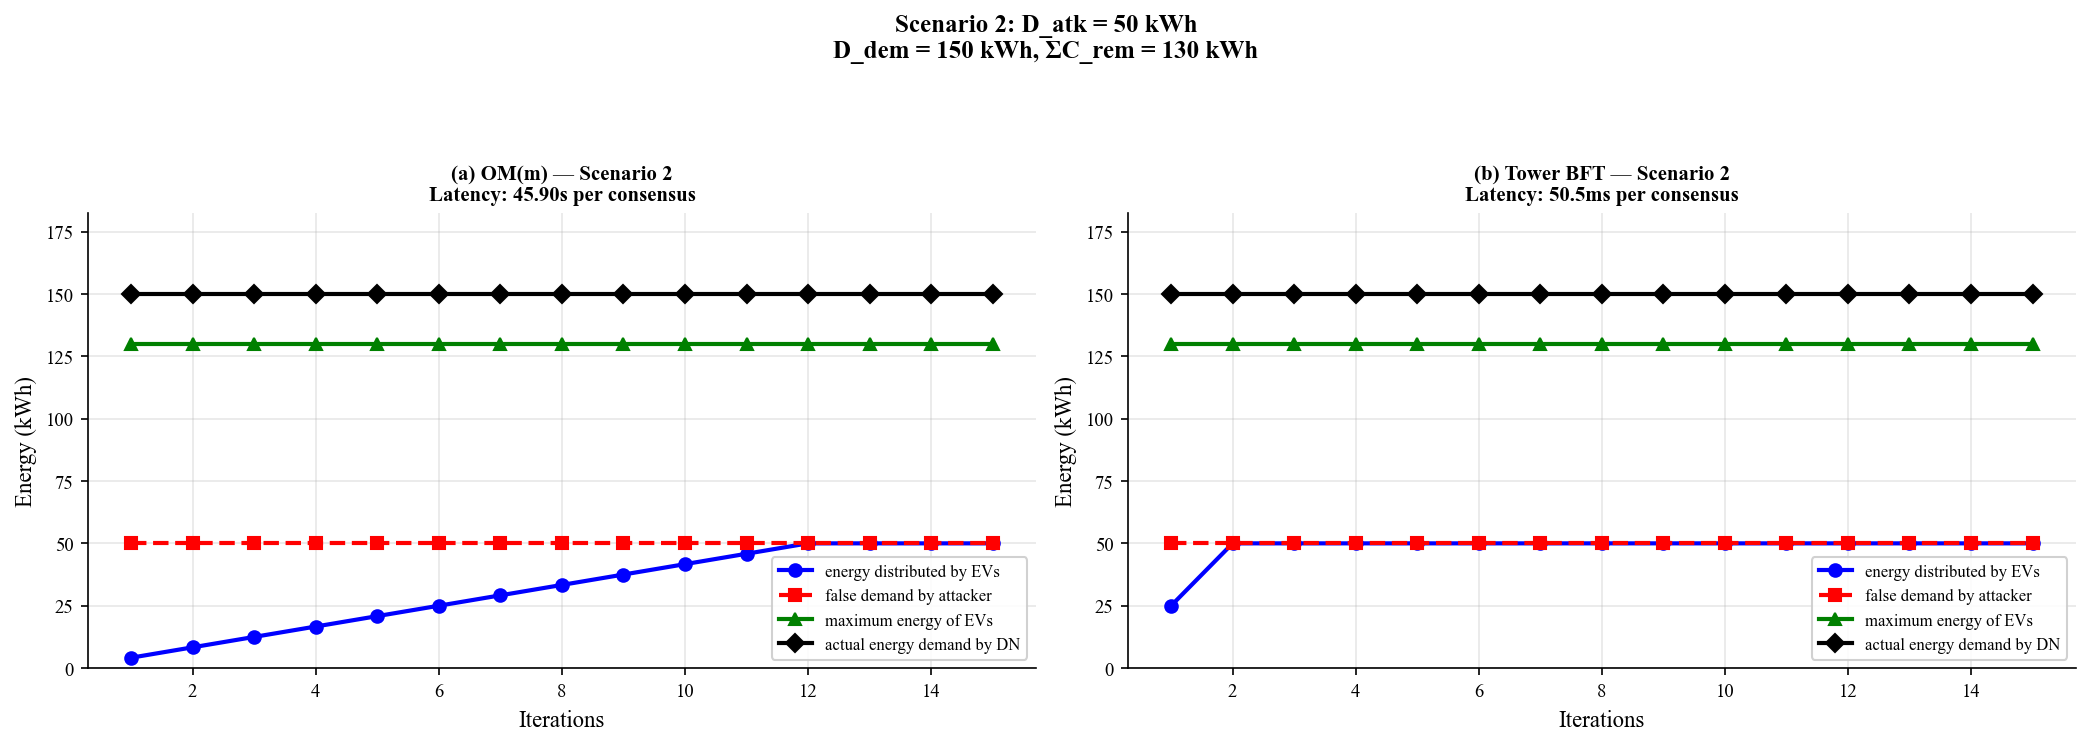
\includegraphics[width=0.75\textwidth]{figures/fig_w2_scenario2_energy.png}
\end{figure}
\clearpage

\section{W Scenario Energy}
\textbf{File:} \texttt{fig\_w2\_scenario3\_energy.png} \\
\textbf{Concept/Origin:} This plot visualizes \textbf{W Scenario Energy Metric} as a function of \textbf{Time / Baseline Parameter}. \\
\textbf{Equations/Framework:} 
 E_{total} = E_{tx} + E_{rx} + E_{crypto} 
\vspace{0.5cm}
\begin{figure}[H]
    \centering
    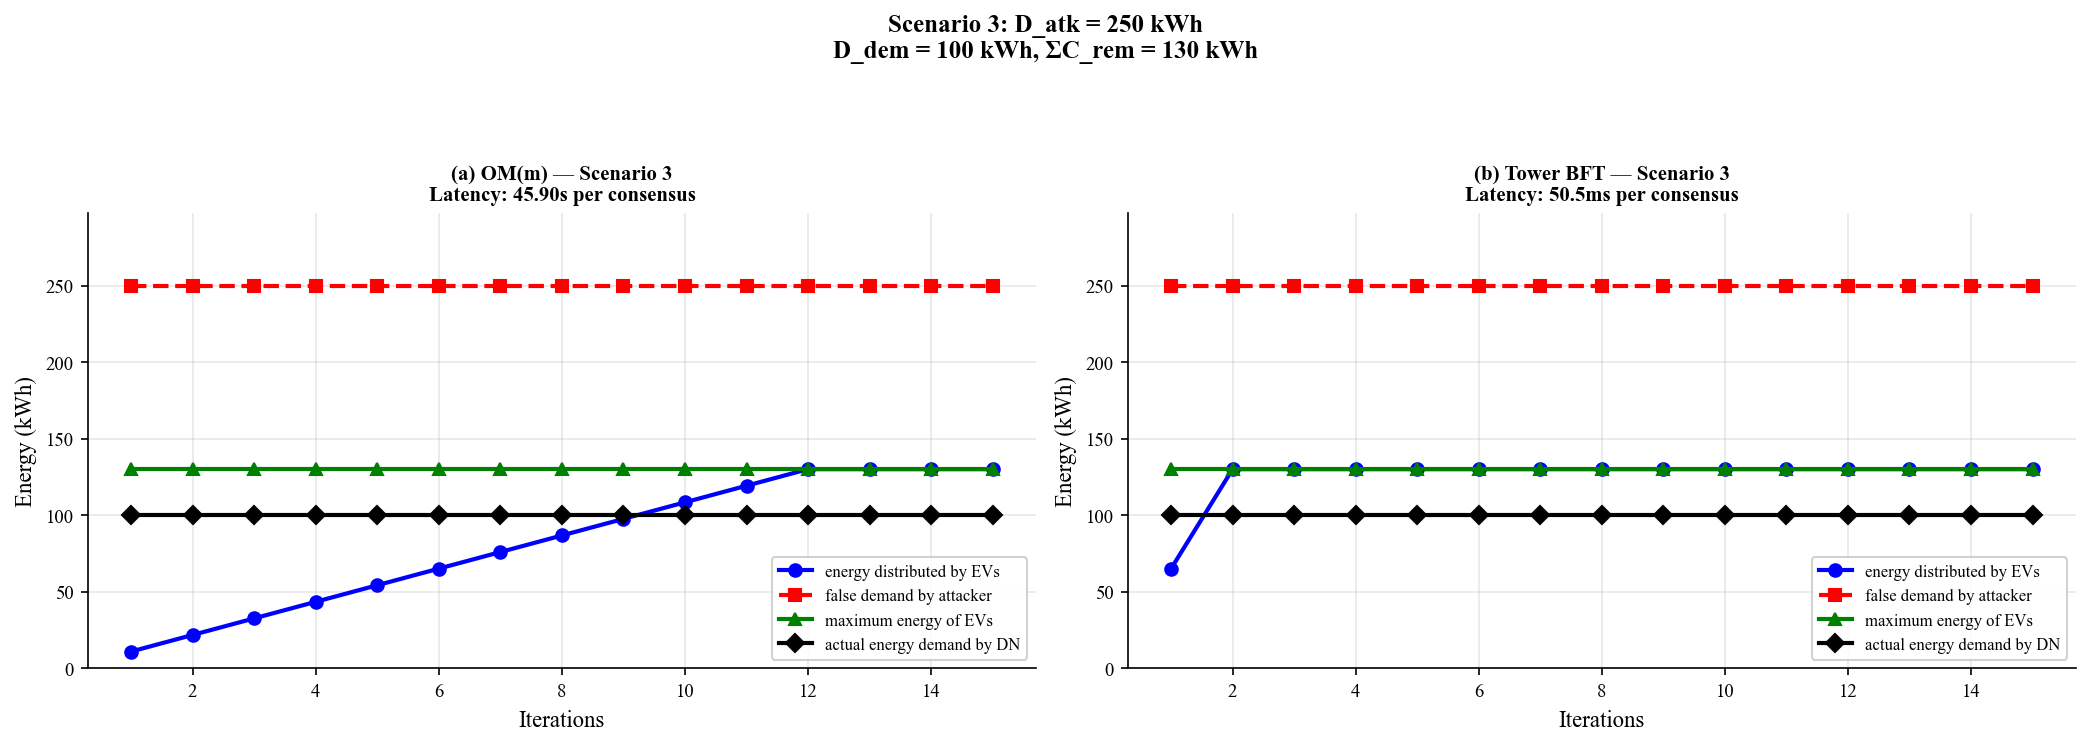
\includegraphics[width=0.75\textwidth]{figures/fig_w2_scenario3_energy.png}
\end{figure}
\clearpage

\end{document}
